% Documents setup
\documentclass[11pt]{book}

% fix for pandoc 1.14
\providecommand{\tightlist}{%
  \setlength{\itemsep}{0pt}\setlength{\parskip}{0pt}}

\usepackage{tabu} % https://tex.stackexchange.com/questions/50332/vertical-spacing-of-a-table-cell

% Location of the csas-style repository: adjust path as needed
\newcommand{\locRepo}{csas-style}

% Use the style file in the csas-style repository (res-doc.sty)
\usepackage{\locRepo/res-doc}

% header-includes from R markdown entry
\usepackage{amsmath}
\usepackage{graphics}

% Headers and footers
\lhead{Draft working paper --- Do not cite or circulate}
% \lhead{}
\rhead{}
% \rfoot{DRAFT - DO NOT CITE}

%%%% Commands for title page etc %%%%%

% Publication year
\newcommand{\rdYear}{2021}

% Publication month
\newcommand{\rdMonth}{Month}

% Report number
\newcommand{\rdNumber}{nnn}

% Region
\newcommand{\rdRegion}{Pacific Region}

% Title
\newcommand{\rdTitle}{Case Study Applications of LRP Estimation Methods to Pacific Salmon Stock Management Units}

\newcommand{\rdISBN}{}
\newcommand{\rdCatNo}{}

% Author names separated by commas and ', and' for the last author in the format 'M.H. Grinnell' (use \textsuperscript{n} for addresses)
\newcommand{\rdAuth}{Kendra Holt\textsuperscript{1} Carrie A. Holt\textsuperscript{2} Luke Warkentin\textsuperscript{1} Catarina Wor\textsuperscript{2} Brooke Davis\textsuperscript{3} others (TBD)\textsuperscript{2}}

% Author names reversed separated by commas in the format 'Grinnell, M.H.'
\newcommand{\rdAuthRev}{Holt, K., Holt, C.A., Warkentin, L., Wor, C. and others(TBD)}

% Author addresses (use \textsuperscript{n})
\newcommand{\rdAuthAddy}{\textsuperscript{1}Institute of Ocean Sciences\\
Fisheries and Oceans Canada, Sidney, Canada\\
\textsuperscript{2}Pacific Biological Station\\
Fisheries and Oceans Canada, 3190 Hammond Bay Road\\
Nanaimo, British Columbia, V9T 6N7, Canada\\
\textsuperscript{3}Delta Regional Office\\
Fisheries and Oceans Canada, 100 Annacis Pkwy Unit 3\\
Delta, British Columbia, V3M 6A2, Canada\\}

\newcommand{\citationOtherLanguage}{Last, F.M. et Smith, A.B. Title Here (\emph{Latin Species Name}). DFO Secr. can. de consult. sci. du MPO. Doc. de rech 2019/nnn. iv + 13 p.}

% Name of file with abstract and resume (see \abstract and \frenchabstract for requirements)
\newcommand{\rdAbstract}{\abstract{The revised fisheries act required that Limit Reference Points (LRPs) be identified for all major fish stocks. For Pacific Salmon, major fish stocks are represented by stock management units (SMUs), which are composed of one or more salmon conservation units (CUs), which are the assessment units under the Wild Salmon Policy. We introduce LRP estimation methods based on aggregating status assessments from the CU level to the SMU level. We demonstrate and evaluate the LRPs for three case study SMUs: Interior Fraser Coho, West Coast Vancouver Island (WCVI) Chinook, and Inner South Coast Chum - excluding Fraser. Methods are divided into two categories: Proportion-based LRPs and Aggregate abundance-based LRPs, which is further sub divided into Logistic regression-based LRPs and Projection-based LRPs. The suitability of each method depends on the availability and quality of data for each SMU, as well as on the historic CU statuses. Proportion-based LRPs are recommended as the default method, while aggregate abundance-based methods are complementary and may be needed to meet management requirements. Proportion-based LRPs are based on individual CU status assessments. Aggregate abundance Logistic regression-based LRPs are based on past status assessments and are estimable when abundance-based CU status is available, and the SMU has observations when the LRP has been breached (at least one CU under red status) and not breached (all CUs above red status). Aggregate abundance Projection-based LRPs are based on future porjections and do not require contrast in previous status observations. However, projections require estimates for population dynamics parameters, as well as estimates of covariation among CUs. We discuss suitability and requirements for the applications of the LRP estimation methods drawing from the range of data and information availability in the study cases.}}

%%%% End of title page commands %%%%%

% \pdfcompresslevel=5 % faster PNGs

\setcounter{section}{0}

\bibliographystyle{csas-style/res-doc}

\usepackage{amsmath}
\usepackage{bm}

% commands and environments needed by pandoc snippets
% extracted from the output of `pandoc -s`
%% Make R markdown code chunks work
\usepackage{array}
\usepackage{amssymb,amsmath}
\usepackage{color}
\usepackage{fancyvrb}

% From default template:
\newcommand{\VerbBar}{|}
\newcommand{\VERB}{\Verb[commandchars=\\\{\}]}
\DefineVerbatimEnvironment{Highlighting}{Verbatim}{commandchars=\\\{\}}
% Add ',fontsize=\small' for more characters per line
\usepackage{framed}
\definecolor{shadecolor}{RGB}{248,248,248}
\newenvironment{Shaded}{\begin{snugshade}}{\end{snugshade}}
\newcommand{\AlertTok}[1]{\textcolor[rgb]{0.94,0.16,0.16}{#1}}
\newcommand{\AnnotationTok}[1]{\textcolor[rgb]{0.56,0.35,0.01}{\textbf{\textit{#1}}}}
\newcommand{\AttributeTok}[1]{\textcolor[rgb]{0.77,0.63,0.00}{#1}}
\newcommand{\BaseNTok}[1]{\textcolor[rgb]{0.00,0.00,0.81}{#1}}
\newcommand{\BuiltInTok}[1]{#1}
\newcommand{\CharTok}[1]{\textcolor[rgb]{0.31,0.60,0.02}{#1}}
\newcommand{\CommentTok}[1]{\textcolor[rgb]{0.56,0.35,0.01}{\textit{#1}}}
\newcommand{\CommentVarTok}[1]{\textcolor[rgb]{0.56,0.35,0.01}{\textbf{\textit{#1}}}}
\newcommand{\ConstantTok}[1]{\textcolor[rgb]{0.00,0.00,0.00}{#1}}
\newcommand{\ControlFlowTok}[1]{\textcolor[rgb]{0.13,0.29,0.53}{\textbf{#1}}}
\newcommand{\DataTypeTok}[1]{\textcolor[rgb]{0.13,0.29,0.53}{#1}}
\newcommand{\DecValTok}[1]{\textcolor[rgb]{0.00,0.00,0.81}{#1}}
\newcommand{\DocumentationTok}[1]{\textcolor[rgb]{0.56,0.35,0.01}{\textbf{\textit{#1}}}}
\newcommand{\ErrorTok}[1]{\textcolor[rgb]{0.64,0.00,0.00}{\textbf{#1}}}
\newcommand{\ExtensionTok}[1]{#1}
\newcommand{\FloatTok}[1]{\textcolor[rgb]{0.00,0.00,0.81}{#1}}
\newcommand{\FunctionTok}[1]{\textcolor[rgb]{0.00,0.00,0.00}{#1}}
\newcommand{\ImportTok}[1]{#1}
\newcommand{\InformationTok}[1]{\textcolor[rgb]{0.56,0.35,0.01}{\textbf{\textit{#1}}}}
\newcommand{\KeywordTok}[1]{\textcolor[rgb]{0.13,0.29,0.53}{\textbf{#1}}}
\newcommand{\NormalTok}[1]{#1}
\newcommand{\OperatorTok}[1]{\textcolor[rgb]{0.81,0.36,0.00}{\textbf{#1}}}
\newcommand{\OtherTok}[1]{\textcolor[rgb]{0.56,0.35,0.01}{#1}}
\newcommand{\PreprocessorTok}[1]{\textcolor[rgb]{0.56,0.35,0.01}{\textit{#1}}}
\newcommand{\RegionMarkerTok}[1]{#1}
\newcommand{\SpecialCharTok}[1]{\textcolor[rgb]{0.00,0.00,0.00}{#1}}
\newcommand{\SpecialStringTok}[1]{\textcolor[rgb]{0.31,0.60,0.02}{#1}}
\newcommand{\StringTok}[1]{\textcolor[rgb]{0.31,0.60,0.02}{#1}}
\newcommand{\VariableTok}[1]{\textcolor[rgb]{0.00,0.00,0.00}{#1}}
\newcommand{\VerbatimStringTok}[1]{\textcolor[rgb]{0.31,0.60,0.02}{#1}}
\newcommand{\WarningTok}[1]{\textcolor[rgb]{0.56,0.35,0.01}{\textbf{\textit{#1}}}}

\newcommand{\lt}{\ensuremath <}
\newcommand{\gt}{\ensuremath >}

%Defines cslreferences environment
%Required by pandoc 2.8
%Copied from https://github.com/rstudio/rmarkdown/issues/1649
\newlength{\cslhangindent}
\setlength{\cslhangindent}{1.5em}
\newenvironment{cslreferences}%
  {}%
  {\par}

\DeclareGraphicsExtensions{.png,.pdf}
\begin{document}

\frontmatter

\hypertarget{introduction}{%
\section{INTRODUCTION}\label{introduction}}

Under DFO's New Fisheries Act, Limit Reference Points (LRPs) will be required for all major fish stocks prescribed in regulation. Stocks that drop below their LRP will trigger the development of a rebuilding plan. For Pacific salmon, it is anticipated there will be \textgreater{} 65 major fish stocks (or stock management units, SMUs), where the proposed functional definition of a SMU is a group of one or more Wild Salmon Policy (WSP) Conservation Units (CUs) that are managed together with the objective of achieving a joint status. Under the WSP, a CU is defined as `a group of wild salmon sufficiently isolated from other groups that, if lost, is very unlikely to recolonize naturally within an acceptable time frame, such as human lifetime or a specified number of salmon generations' (\protect\hyperlink{ref-dfoCanadaPolicyConservation2005}{\emph{Canada's {Policy} for {Conservation} of {Wild} {Pacific} {Salmon}} 2005}). Thus, while LRPs under the Fisheries Act are required at the SMU-level, monitoring and management under DFO's WSP occurs at the finer CU-level. Methods to assess CU status have been identified for a range of data types, and WSP Integrated Assessment methods (hereafter called `WSP assessments') that use expert opinion to combine multiple metrics into a single estimate of CU status have been developed (e.g., \protect\hyperlink{ref-grant2017FraserSockeye2020}{Grant et al. 2020}). Metrics used to assess WSP CU status include spawner abundances, short- and long-term trends in abundance, and distribution of abundance. Lower and upper benchmarks on those metrics are used to assign status into one of three zones, green, amber and red, representing increasingly depleted population and requiring increased management interventions (DFO 2005), and are described more fully in the companion paper to this one, \emph{Guidelines for Defining Limit Reference Points for Pacific Salmon Stock Management Units} (Holt et al., in review). At present, a key gap in our ability to develop LRPs under the Fisheries Act is that CU-level status assessments have not been aggregated to the SMU level.

LRPs are defined within DFO's `Precautionary Approach to Fisheries Decision-Making' as the stock status below which serious harm is occurring to the stock (\protect\hyperlink{ref-governmentofcanadaFisheryDecisionmakingFramework2009}{Government of Canada 2009}). While LRPs are often based on metrics directly linked to productivity, such as spawning biomass or fishing mortality rates, the type of metric used to define an LRP can vary among species and data types, and may be related to other stock characteristics when appropriate. Since the CU is the fundamental unit of biodiversity that DFO aims to maintain under the WSP, it follows that methods for identifying LRPs should ensure that component CUs are maintained. Our companion paper, Holt et al., (in review) argues that the maintenance of spawning abundance at the CU level is a key biological requirement for Pacific Salmon LRPs.

The goals of this working paper are to demonstrate alternative LRP estimation methods for three case study SMUs that vary in data types and availabilities, and then evaluate candidate LRPs using a combination of sensitivity analyses and, where possible, retrospective analyses. A full evaluation of LRPs, for examples, using closed-loop simulations, is beyond the scope of the current project and is a high priority for future research. The case studies considered were Interior Fraser Coho Salmon (\emph{Oncorhynchus kisutch}), West Coast Vancouver Island (WCVI) Chinook Salmon (\emph{Oncorhynchus tshawytscha}), and Inner South Coast Chum Salmon (\emph{Oncorhynchus keta}) - excluding Fraser. Each of these SMUs is comprised of 3-7 CUs and has been selected to represent a different level of data availability ranging from data rich (Interior Fraser Coho) to data-limited (Inner South Coast Chum). Detailed guidelines for identifying LRPs for Pacific salmon SMUs informed by these three case study applications are available in the companion working paper (Holt et al., in review). For each case study, the set of LRP estimation methods considered is a function of available data and previously developed assessment methods for the SMU. The LRPs presented in this paper are illustrative and not meant to be definitive, as they may require more thorough review of data and methodology with local analysts and partners.

\hypertarget{MethodsChapter}{%
\section{LRP ESTIMATION METHODS}\label{MethodsChapter}}

In this section, we provide an overview of methods used to develop LRPs for our three case studies. Detailed methods specific to each case study are provided in Sections 3 (Interior Fraser Coho), 4 (WCVI Chinook), and 5 (Inner South Coast Chum, excluding Fraser).

\hypertarget{overview}{%
\subsection{OVERVIEW}\label{overview}}

We consider two types of LRPs based on two different metrics:
\begin{enumerate}
\def\labelenumi{\arabic{enumi})}
\item
  Proportion-based LRPs, which are based on the proportion of CUs within an SMU that are assessed as being above the red WSP status zone. We assume that in order for an SMU to remain above its proportion-based LRP, 100\% of CUs must have status estimates above red (i.e., either amber or green).
\item
  Aggregate abundance-based LRPs, which are based on total SMU-level spawning abundance.
\end{enumerate}
While aggregate abundance-based LRPs are consistent with what is typically used for marine fish species, proportion-based LRPs have been proposed for Pacific salmon to align with DFO's Wild Salmon Policy.

WSP assessments are typically intensive expert-driven processes and have only been completed for a small subset of CUs to date. We demonstrate the application of a rapid multidimensional scanning tool that is being developed by DFO's State of the Salmon Program to rapidly assess CU status under the WSP (Pestal et al., in prep). Applying this tool allows us to generate up-to-date estimates of CU status for all of our case study applications, and is recommended as a tool for defining LRPs in our companion working paper (Holt et al., in review). When developing aggregate abundance-based LRPs, we also consider cases in which CU status is based on spawning abundance relative to a single lower benchmark that has been identified as important by local experts. While the rapid multidimensional scanning tool better captures the multiple dimensions that are used to inform biological status under the WSP (e.g., abundances, short-term and long-term trends), we compare it to status derived from a single metric relative to a lower benchmark to demonstrate how in many cases the rapid multidimensional scanning tool reduces to this metric. Exceptions are described in the application to case studies. A variety of methods are available for estimating lower benchmarks on abundances depending on species and data availability (\protect\hyperlink{ref-holtIndicatorsStatusBenchmarks2009}{Holt et al. 2009}; \protect\hyperlink{ref-grant2017FraserSockeye2020}{Grant et al. 2020}; \protect\hyperlink{ref-holtEvaluatingBenchmarksBiological2018}{\textbf{holtEvaluatingBenchmarksBiological2018?}}), as described in Holt et al.~(in review).

When developing aggregate abundance-based LRP options for salmon SMUs, we aim to maintain consistency with the WSP by defining LRPs as aggregate abundance levels that have a high probability of all CUs being above red status. We use two different methods to identify these levels: (i) Logistic regression-based LRPs and (ii) Projection-based LRPs. More detailed descriptions of these methods are provided in the following sections, while guidance on when and how proportion-based and aggregate abundance-based LRPs should be applied is provided in Holt et al.~(in review). We do not recommend that users apply any of the methods described in this case study paper without first consulting Holt et al.~(in review). While aggregate-abundance based LRPs can be used to inform harvest control rules for fisheries management, more complex harvest control rules that include for example, time-area closures to limit CU-specific harvests may better achieve the underlying objective of maintaining CU statuses above red (as described in Holt et al.~(in review))

\hypertarget{proportion-based-lrps}{%
\subsection{PROPORTION-BASED LRPS}\label{proportion-based-lrps}}

A proportion-based LRP is simply the proportion of CUs required to be assessed as being above red status. In all three case studies, we default to 100\% of CUs being required to be above red status when setting the LRP. In this case, the LRP acts as a trigger that is breached when one of more CUs is assessed as having red status. Rationale for the choice of 100\% of CUs required to be above red status in order for an SMU to be considered above its LRP is described in (Holt et al.~in review).

We compare three different methods of assessing CU status when using proportion-based LRPs: (i) the proportion of CUs with a recent WSP status assessment above the red zone (e.g., \protect\hyperlink{ref-grant2017FraserSockeye2020}{Grant et al.} (\protect\hyperlink{ref-grant2017FraserSockeye2020}{2020})), (ii) the proportion of CUs with a recent rapid multidimensional status assessment above red (see below for more details), and (iii) the proportion of CUs with status estimated to be below a single type of CU lower benchmark (e.g., \(S_{gen}\), percentile-based benchmarks, etc.). While we recommend applying methods (i) or (ii), approach (iii) is shown for comparison purposes to demonstrate consistency between rapid multidimensional status assessments and statuses derived from abundances relative to lower benchmarks.

When assessing CU status relative to a single abundance-based lower benchmark in approach (iii), we use generational mean spawner abundances as a basis for determining whether each CU is above or below its lower benchmark. Generational smoothing integrates status over cohorts within a generation, which are generally independent of each other because of the anadromous, semelparous life-history of Pacific salmon and the dominance of a single age-at-maturity for many stocks. This approach reduces noise in annual CU status determination due to annual fluctuations in CU abundances from any single cohort. It also makes our determination of CU status consistent with the approach taken for abundance-based benchmarks in WSP assessments and the rapid multidimensional scanning tool.

\hypertarget{rapidToolMethods}{%
\subsubsection{Rapid Multidimensional Scanning Tool}\label{rapidToolMethods}}

One of the methods we consider to estimate CU status for proportion-based LRPs relies on a method of rapidly assessing CU status using multidimensional algorithms. We implement this approach using a scanner tool that has recently been developed by DFO's State of the Salmon Program (\protect\hyperlink{ref-pestalAlgorithmsRapidStatus2021}{Pestal et al.} (\protect\hyperlink{ref-pestalAlgorithmsRapidStatus2021}{2021}), in prep) . The scanning tool is intended to support implementation of Canada's WSP by approximating the outcomes of full WSP Integrated Status Assessments on an more regular basis than the time-intensive WSP assessment approach allows. The rapid multidimensional scanning tool was developed using Classification and Regression Tree (CART) analyses to create algorithms that approximate the status of the integrated assessments. Data inputs and outcomes from the WSP assessment processes were used in CART analyses: Fraser River sockeye, Interior Fraser coho, and Southern BC Chinook (\protect\hyperlink{ref-dfoWildSalmonPolicy2015}{DFO 2015}; \protect\hyperlink{ref-dfoIntegratedBiologicalStatus2016}{DFO 2016}, \protect\hyperlink{ref-dfo2017FraserSockeye2018}{2018}; \protect\hyperlink{ref-grant2017FraserSockeye2020}{Grant et al. 2020}), and was further ground-truthed with data for Fraser River Chum and Pink Salmon (Pestal et al.~in prep ). . Briefly, the scanning tool uses a decision tree to estimate CU status based on data type, quality, abundance, and trends (e.g., Figure~\ref{fig:decision-tree}). An expert review of rapid status results for each CU is intended to be incorporated into application of this tool (S. Grant, pers comm). When using this method in the case study, we took the outputs of the algorithms at face value and did not confirm them based on expert opinion.

\newpage
\begin{landscape}
\begin{figure}[htb]

{\centering \pdftooltip{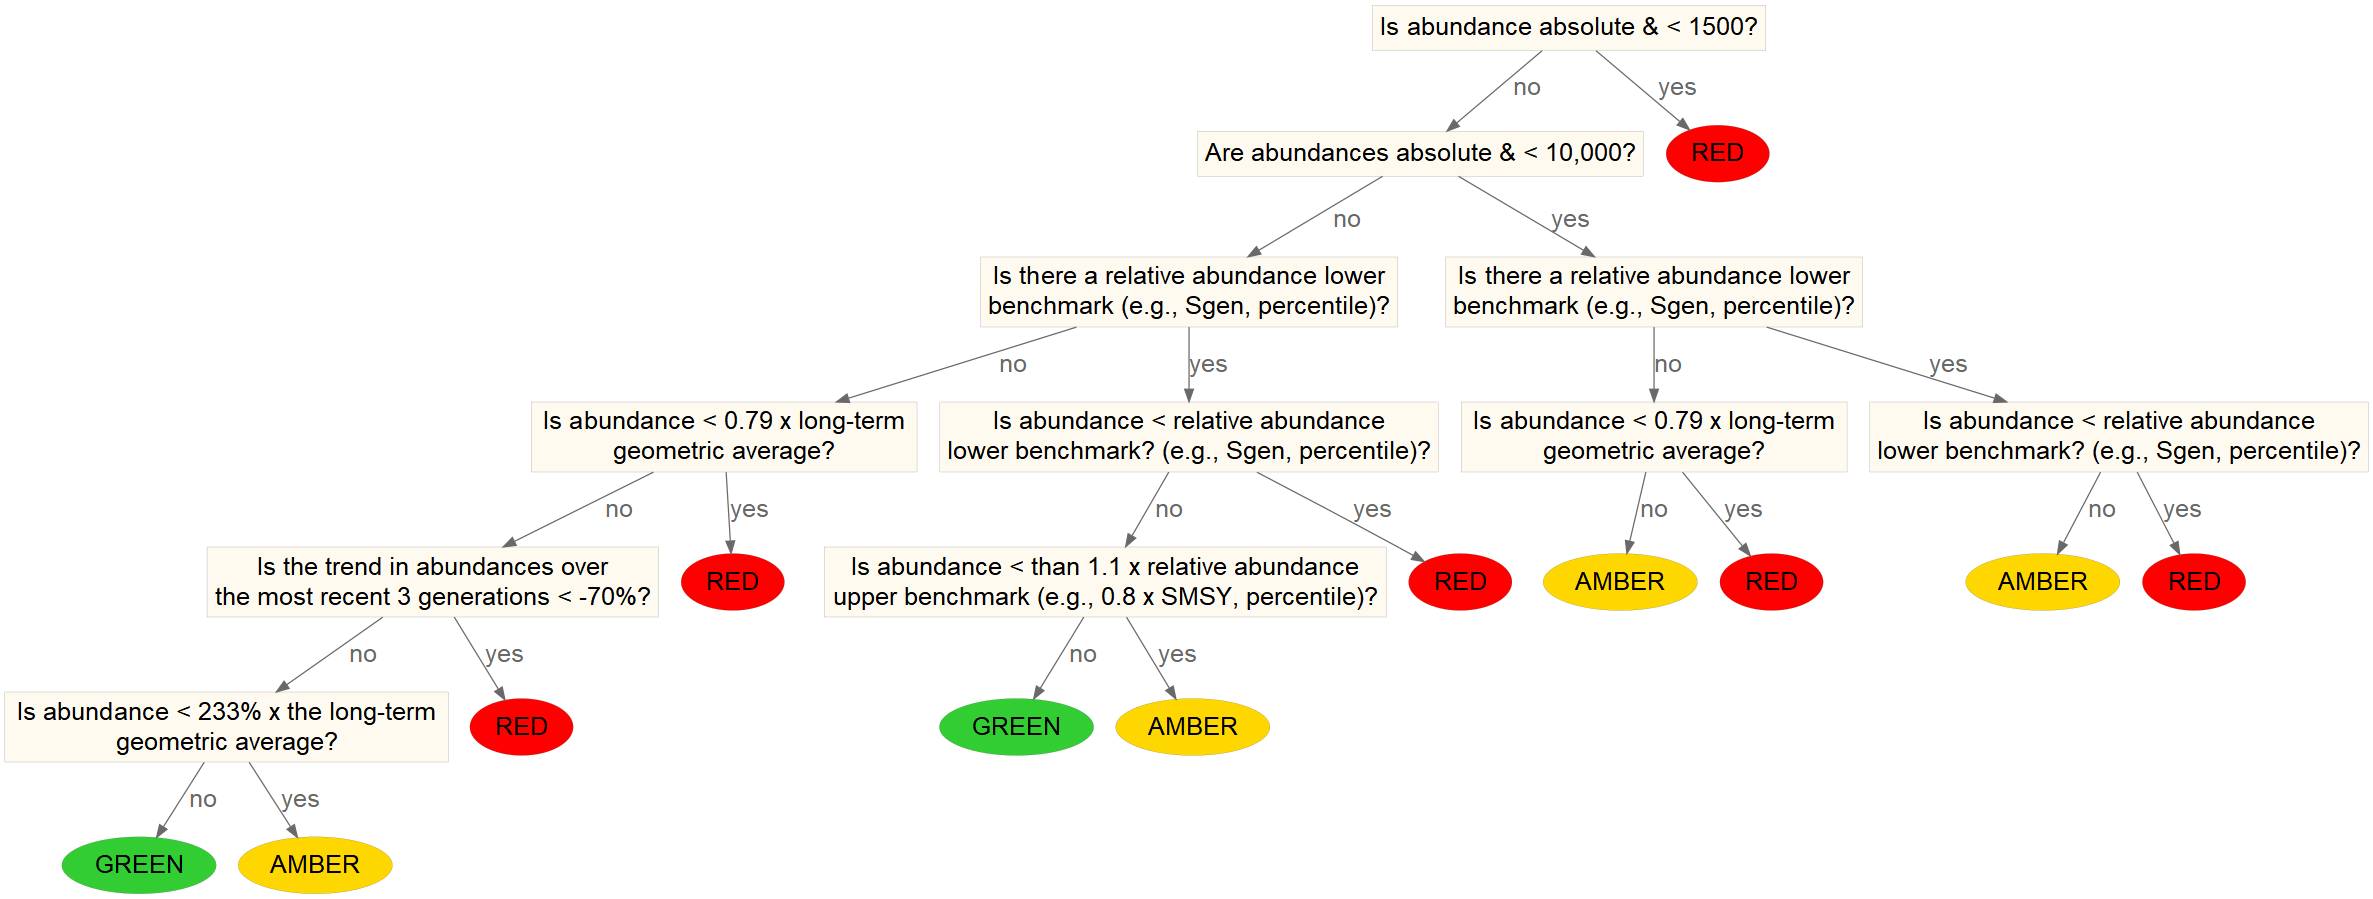
\includegraphics[width=1\linewidth]{figure/decision_tree}}{Figure \ref{fig:decision-tree}} 

}

\caption{Decision tree to assess status of Conservation Units based on the Wild Salmon Policy, under development by State of the Salmon Program}\label{fig:decision-tree}
\end{figure}
\end{landscape}
The rapid multi-dimensional scanning tool uses generational mean spawner abundances as a basis for comparison at each node of the decision tree, including when comparing against absolute abundance thresholds (e.g., 1500 spawners), abundance-based lower benchmarks (e.g., \(S_{gen}\) or percentile), and abundance-based upper benchmarks (e.g., 0.8\(S_{MSY}\) or percentile). Spawner abundances are also smoothed using generational averages prior to calculating trends in spawner abundance over time (Pestal et al., in prep).

\hypertarget{aggAbundMethods}{%
\subsection{AGGREGATE ABUNDANCE-BASED LRPS}\label{aggAbundMethods}}

Aggregate abundance-based LRPs are based on the SMU-level abundance at which there is a sufficiently high probability that 100\% of CUs (the same \% as used for proportion-based LRPs) will be above a single selected benchmark. When developing aggregate abundance-based LRPs, status relative to a single benchmark is used a proxy for above the red zone. The Rapid Multidimensional Scanner Tool was considered in preliminary analyses as way to identify `red' status for aggregate-abundance based LRPs, but we dismissed it for computational reasons that are described below. The above definition of aggregate abundance-based LRPs requires a decision to be made about what represents a `sufficiently high probability' that 100\% of CUs will be above their benchmarks. We consider four alternative probability levels for our case studies that represent a range of calibrated probability categories developed by the Intergovernmental Panel on Climate Change (\protect\hyperlink{ref-frameGuidanceNoteLead2010}{Frame et al. 2010}): 50\%, 66\%, 90\%, and 99\%. The 50\% value represents the mid-point of the ``About as likely as not'' category (33 - 66\%), indicating that there is an equal probability that all CUs will be above their LBMs as there is that they will not. The 66\% values represents the lower end of the ``Likely'' category (i.e., it is ``Likely'' that all CUs will be above their LBMs), the 90\% value represents the lower end of the ``Very Likely'' category, and the 99\% value represents the ``Virtually Certain'' category. A discussion of considerations for selecting the appropriate probability threshold when calculating abundance-based LRPs is included in (Holt et al.~in review).

We consider two types of aggregate abundance-based LRPs in our case studies: Logistic regression-based LRPs and Projection-based LRPs. Logistic regression LRPs are estimated using historical data, representing conditions that have been previously experienced by a SMU and thus implicitly assume the past is a reasonable approximation of the future. In comparison, projection-based LRPs use historical data as a basis for quantifying population dynamics, but are based on projections of future states, and thus, allow uncertainty in future processes to be accounted for through alternative scenarios. Thus projection-based LRPs overcomes one key short-coming of the logistic-regression based LRP that historical conditions might not represent current (or future) conditions, by allowing the user to specify model structure and parameter estimates and their uncertainties that reflect the best-available science on current (or future) dynamics.

Within both the logistic regression- and projection-based LRP estimation routines, we characterize annual CU status using a single metric, spawner abundances relative to benchmarks instead of using the Rapid Multidimensional Scanner Tool as in the proportion-based LRPs. While in theory, estimates of CU status used in the aggregate-abundance based methods could be derived from the rapid multidimensional scanning tool, we found little evidence of a statistical relationship between between multidimensional CU status and aggregate spawner abundance for the one case study we considered this approach for: Interior Fraser Coho. In addition, projection-based LRPs are derived from an equilibrium model that does not incorporate temporal dynamics required for assessment of trends in the Rapid Multidimensional Scanner Tool. As a result, we rely on status estimated from a single lower benchmark metric (e.g., \(S_{gen}\)) rather than the multidimensional scanner tool to develop aggregate-abundance based LRPs in our case studies. We provide further discussion of this result within the Interior Fraser Coho case study section of this paper.

In addition, we characterize annual CU status using raw annual spawner abundances instead of generational averages when estimating aggregate abundance-based LRPs. This approach is based on preliminary analyses of the logistic regression-based method that showed using raw spawner abundances improved the spread in the data used to establish a relationship between CU status and aggregate spawning abundance. Furthermore, using generational means in the logistic regression-based approach led to considerable autocorrelation in the aggregate abundance time series, violating assumptions of the logistic regression. We therefore used raw annual spawner abundances within the estimation routines for aggregate-abundance based LRPs. However, we used generational averages of aggregate spawner abundances when assessing SMU-level status relative to the aggregate abundance-based LRPs to reduce noise in annual decisions about whether an LRP had been breached related to variability in cohorts within a generation. The decision to use generational averages of aggregate spawner abundances when determining whether an LRP is breached is consistent with the approach used for proportion-based LRPs. In both cases, the underlying metric being used to determine SMU status (either aggregate abundance or CU-level status of component CUs for the proportion-based approach) is based on generational-averaged values in order to reduce annual fluctuations in status related to independent cohorts within a generation.

\hypertarget{logisticMethods}{%
\subsubsection{Logistic regression-based LRPs}\label{logisticMethods}}

Logistic regression-based LRPs (also called Logistic regression LRPs) are derived from an empirically estimated relationship between CU-level status and aggregate SMU abundance. Using this approach, the LRP represents the aggregate abundance level that has historically been associated with a given probability of 100\% of CUs having status above a selected lower benchmark. For each year of observed data, CU-level status is quantified as a Bernoulli variable: 1 (success) = all CUs have estimated status greater than their lower benchmark (LBM) and 0 (failure) = all CUs did not have status \textgreater{} LBM. A logistic regression is then fit to these outcomes to predict the probability that all CUs will have status \textgreater{} LBM as a function of aggregate SMU spawner abundance using the logistic regression equation:
\begin{equation}
  \log(\frac{p}{1-p}) = B_0 + B_1 \sum_{i}^{i=nCUs} S_{i,t}
   \label{eq:logistic}
\end{equation}
where, \(p\) is probability, \(B_0\) and \(B_1\) are estimated logistic regression parameters and \(S_{i,t}\) is spawner abundance to CU \(i\) in year \(t\). Equation~\ref{eq:logistic} is then re-arranged to calculate the LRP as the aggregate spawner abundance associated with the pre-specified probability threshold of \(p^*\),
\begin{equation}
  LRP = \frac{log(\frac{p^*}{1-p^*}) - B_0}{B_1}
  \label{eq:logisticLRP}
\end{equation}
Annual spawner abundances at both the CU and SMU level for this analysis are on the raw scale (i.e., no generational averaging applied). An example logistic regression fit is shown in Figure~\ref{fig:example-logisticFit}. We show the estimation of LRPs based on this fit for four possible probability thresholds: \(p^*\) = 0.5, 0.66, 0.90, and 0.99. For each \(p^*\) level, LRP estimates represent the aggregate abundance that is associated with that probability of all CUs having status greater than their LBM. Logistic regression models were fit using TMB (citation), with resulting LRP estimates from equation~\ref{eq:logisticLRP} calculated within the code. Uncertainty in LRP estimates were quantified based on a 95\% confidence interval on the maximum likelihood estimate, MLE.
\begin{figure}[htb]

{\centering \pdftooltip{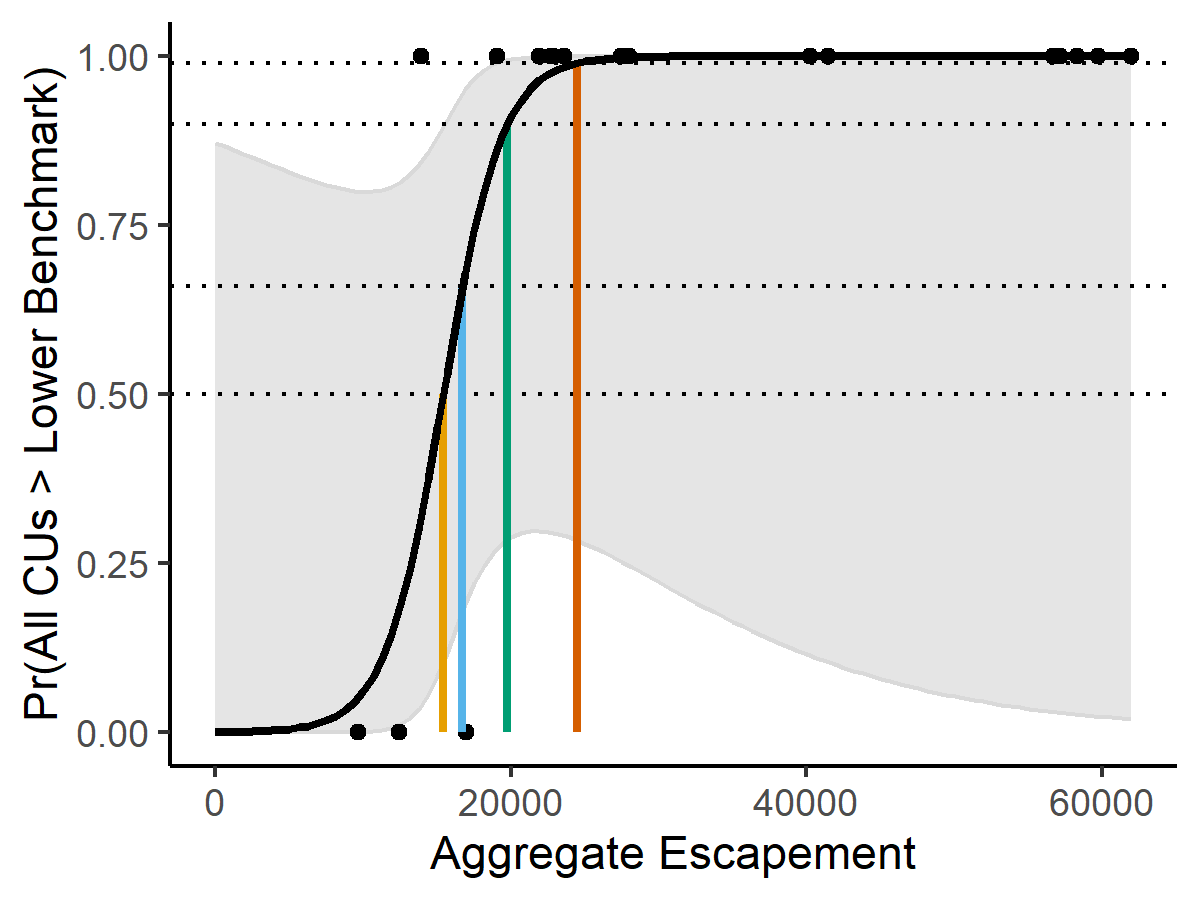
\includegraphics[width=0.6\linewidth]{figure/methods-Example-LogisticLRP}}{Figure \ref{fig:example-logisticFit}} 

}

\caption{Logistic regression fit to annual Bernoulli data to predict the probability of all CUs being above their lower benchmark (LBM) as a function of aggregate SMU abundance. Each black dot represent a year in the observed time series as a Bernoulli indicator showing whether the requirement of all CUs above their LBM was met (success = 1) or not (failure = 0) as a function of aggregate spawning abundance to the SMU. The black solid line is the maximum likelihood model fit to indicator data, and the grey shaded region shows the 95\% confidence interval around the fit model. Coloured lines illustrate aggregate abundance LRPs for 4 different probability thresholds: p* = 0.5 (yellow), 0.66 (blue), 0.90 (green), and 0.99 (orange) probability that all CUs > LBM. Horizontal dotted lines intersect the y-axis at each probability threshold, while the solid vertical lines show the corresponding aggregate escapement that will represent the LRP.}\label{fig:example-logisticFit}
\end{figure}
We initially considered an alternative approach to logistic regression in which the LRP represents the aggregate abundance that has historically been associated with a pre-specified proportion of CUs being above their lower benchmark. Using this approach, CU-level status was quantified as the number or CUs with status \textgreater{} LBM for each year of observed data. A logistic regression was then fit to predict the proportion of CUs with status \textgreater{} LBM as a function of aggregate spawner abundance to the SMU (i.e., abundance from nCUs combined). We do not present this method for our case studies, however, due to inherent limitations when the required proportion of CUs above their lower benchmarks is 100\%. Equation~\ref{eq:logisticLRP} cannot be solved directly for a threshold proportion of \(p^*\) = 100\%, and LRP estimates were highly sensitive to the choice of \(p^*\) value used as a proxy. Using \(p^*\) = 99\% vs.~\(p^*\) = 99.9\% vs.~\(p^*\) = 99.99\% gave very different LRP estimates.

The logistic regression model was implemented in TMB (\protect\hyperlink{ref-kristensen_tmb_2016}{\textbf{kristensen\_tmb\_2016?}}). The model was statistically integrated, i.e., both the CU-specific lower benchmarks (\(S_{gen}\)) and the SMU logistic regression parameters were estimated within the same statistical model. The integrated approach allowed the propagation of uncertainty in parameter estimates from the CU level to the SMU level resulting in more comprehensive uncertainty estimates for the aggregate abundance LRPs.\\

\hypertarget{logistic-regression-model-diagnostics}{%
\paragraph{Logistic Regression Model Diagnostics}\label{logistic-regression-model-diagnostics}}

There are several assumptions associated with logistic regression, three of which are relevant for our application to LRPs are listed below. Model diagnostics were applied to evaluate the extent to which those assumptions were met, as well as statistical significance of model coefficients, goodness-of-fit, and classification accuracy of LRPs developed from the logistic regression. The three assumptions are as follows:
\begin{enumerate}
\def\labelenumi{\arabic{enumi}.}
\item
  The relationship between aggregate abundance and log-odds (the logarithm of the odds of all CUs being above their lower benchmark) is linear.
\item
  The observations are independent of each other (i.e., residuals are not autocorrelated).
\item
  There are no influential outliers.
\end{enumerate}
\textbf{Evaluating assumption of linearity (Assumption 1)}

A Box-Tidwell test was used to evaluate linearity by assessing the significance of an additional interaction term in the logistic regression,
\begin{equation}
  \log(\frac{p}{1-p}) = B_0 + B_1 \sum_{i}^{i=nCUs} S_{i,t} + B_2 \sum_{i}^{i=nCUs} S_{i,t} \times \log (\sum_{i}^{i=nCUs} S_{i,t})
   \label{eq:BoxTidwelllogistic}
\end{equation}
A significant interaction term \(B_2\), indicates a non-linear relationship between aggregate abundance and log-odds, violating this assumption (\protect\hyperlink{ref-foxAppliedRegressionAnalysis2016}{Fox 2016}).

\textbf{Evaluating independence (Assumption 2)}

Deviance residuals, \(d\), were estimated for each year,
\begin{equation}
   d = \pm \sqrt { -2 ( y \log(\frac{\mu}{y}) + (1-y)\log(\frac{1-\mu}{1-y}) ) }
   \label{eq:DevianceResid}
\end{equation}
where \(\mu\) is the predicted probability of all CUs being above their lower benchmark and \(y\) is the observation (1 or 0, indicating all CUs above red or not, respectively), in a given year (\protect\hyperlink{ref-foxAppliedRegressionAnalysis2016}{Fox 2016}). Equation~\ref{eq:DevianceResid} reduces to (\protect\hyperlink{ref-ahmadDiagnosticResidualOutliers2011}{Ahmad 2011}):
\begin{align}
d = 
\begin{cases}
  - \sqrt { -2 \log(1-\mu) } & \text{, if } y = 0 \\
  \sqrt { -2 \log(\mu)  }  &\text{, if } y = 1
\end{cases}
  \label{eq:DevianceResidy}
\end{align}
The magnitude of lag-1 autocorrelation was then estimated among deviance residuals and evaluated for statistical significance.

\textbf{Evaluating outliers (Assumption 3)}

We recommend identifying influential outliers using leverage statistics where possible. For our case studies, we identified outliers independent of their influence because the software used to estimate model parameters (TMB) does not provide the hat-matrix required to assess influence of individual points. Instead, we focused on identifying outliers based on the general rule of thumb that deviance residuals greater than 2 are considered to be to be outliers because 95\% of the distribution is expected to be within 2 standard deviations of the mean. Further work to identify influential outliers is recommended when other statistical model fitting tools are used.

\textbf{Statistical significance of model coefficients}

Statistical significance of coefficients was evaluated using the Wald test statistic, calculated from the ratio of the model coefficient to the standard error of that coefficient, which is assumed to be normally distributed. Test statistics and significance were estimated within TMB (\protect\hyperlink{ref-kristensenTMBAutomaticDifferentiation2016}{Kristensen et al. 2016}).

\textbf{Goodness-of-fit}

The goodness-of-fit was evaluated by comparing the ratio of residual deviance to null deviance (similar to a likelihood ratio). This ratio is assumed to follow a Chi-square distribution with 1 degree of freedom derived from the difference in the number of parameters between full and null models (1). P-values \textless0.05 indicate significant lack of fit (\protect\hyperlink{ref-foxAppliedRegressionAnalysis2016}{Fox 2016}).

In addition, the pseudo-\(R^2\) was calculated to indicate the ratio of the model fit to the null model without an independent variable (\protect\hyperlink{ref-dobsonIntroductionGeneralizedLinear2018}{Dobson and Barnett 2018}),
\begin{equation}
   \text{pseudo-}R^2 =  1- \frac{\sum_{t}^{t=nYears} d}{\sum_{t}^{t=nYears} d_0} 
   \label{eq:psuedoR2}
\end{equation}
where \(d_0\) are the deviance residuals for the null model. The psuedo-\(R^2\) is a measure of the strength of the relationship between aggregate abundances and probability of all CUs being above their lower benchmarks, but unlike \(R^2\) values for linear models, it does not represent the percentage of variance explained by the model and is not related to the correlation coefficient.

In addition, the length of available time-series will impact power to detect significant model coefficients, and coefficient estimates may be biased when time-series are short. \protect\hyperlink{ref-peduzziSimulationStudyNumber1996}{Peduzzi et al.} (\protect\hyperlink{ref-peduzziSimulationStudyNumber1996}{1996}) recommend a minimum of 10 data points for the least frequent outcome to avoid biases in model coefficients, based on simulation study of epidemiological data. For example, if the frequency of outcomes were 0.5 and 0.5 (for 0 and 1, respectively), then a sample size of at least 10/0.5 = 20 would be sufficient, and this minimum sample size would be higher if the data were skewed, e.g., if frequency of outcomes were 0.7 and 0.3, the minimum sample size would be 10/0.3 = 33. A similar evaluation of sample sizes to minimize biases logistic-regression based LRPs for fisheries applications is warranted. Although it is possible to estimate LRPs with lower sample sizes, the risks of biases in model parameters (and LRPs) increases.

\textbf{Classification accuracy of LRPs}

Classification accuracy was evaluated based on the ratio of successful classifications to total number of data points in the logistic regression, also called the hit ratio. Successful classifications were the number of years when the model successfully predicted that all CUs were above their lower benchmark plus the number years when the model successfully predicted that at least one CU was below its lower benchmark. The hit ratio tends to be biased towards optimistic classification rates when computed with the same sample used for fitting the logistic model. Therefore, we also considered an out-of-sample approach to classification accuracy, where the logistic regression was estimated iteratively removing a single data point and the occurrence of successes relative to observations were based on the model that did not contain that data point.

\hypertarget{projectedMethods}{%
\subsubsection{PROJECTION-BASED LRPS}\label{projectedMethods}}

The projection-based LRP approach uses population parameters of individual CUs within an SMU to project abundances forward with natural variability in recruitment and ages-at-maturity under current exploitation rates characterized with annual implementation uncertainty. Projections are run for 30 years after an initialization period to remove the impacts of initial conditions and identify aggregate abundances characterized by an equilibrium state represented by stable distribution of projected abundances. Projection-based LRPs are then estimated using these projected CU abundances to characterize the relationship between aggregate SMU-level spawner abundance and the probability that all CUs will be above their lower benchmarks (e.g.~\(S_{gen}\)). This projection-based LRP approach allows for explicit consideration of uncertainty as the user can specify various projection scenarios to reflect a lack of biological and/or fisheries information. As with logistic regression-based LRPs, we relied on status estimated from a single metric rather than the multidimensional scanner tool to develop LRPs using projections.

We used the samSim closed loop simulation modelling tool to conduct stochastic projections for our case study applications. samSim is an R package that was developed to quantify recovery potential for Pacific salmon populations (\protect\hyperlink{ref-holtQuantitativeToolEvaluating2020}{Holt et al. 2020}; \protect\hyperlink{ref-freshwaterBenefitsLimitationsIncreasing2020}{Freshwater et al. 2020}). We created a modified version of samSim to support LRP estimation. The LRP version of samSim is described in detail in Appendix~\ref{app:samsim-appendix}, and model code is available on GitHub at: \url{https://github.com/Pacific-salmon-assess/samSim/tree/LRP}.

Detailed descriptions of the parameterization of samSim for our two case study applications of abundance-based projected LRPs (Interior Fraser Coho and WCVI Chinook) are presented in Chapters 3 and 4, respectively. In both cases, we incorporated uncertainty into projected CU dynamics through the specification of empirically-derived probability distributions for key biological and management parameters, including stock-recruitment parameters, proportion of recruits at age, and exploitation rates (ER). Larger structural uncertainties in model formulation were represented through the use of sensitivity analyses and/or alternative operating models (OMs). Observation error was not included in projections because derivation of LRPs was based on projected `true' abundance levels rather than observed abundance.

The following steps were taken to calculate projection-based LRPs:
\begin{enumerate}
\def\labelenumi{\arabic{enumi}.}

\item
  Use samSim to project spawner abundances forward for \(nYears\) over \(nTrial\) stochastic simulations, under current exploitation.
\end{enumerate}
\begin{enumerate}
\def\labelenumi{\arabic{enumi}.}
\setcounter{enumi}{1}
\item
  For each simulated year-trial combination, characterize abundances as follows:
  \begin{itemize}
  \item
    Assign aggregate SMU level spawner abundance for each year-trial combination to an abundance bin (\(AggS_{bin}\)), based on intervals of 200 fish . E.g., \(AggS_{bin}\) = 0:200 fish, 201:400 fish, 401:600 fish, \ldots{} etc.
  \item
    Determine whether all CUs for that year-trial combination were above their CU-level lower benchmarks on abundances. If they were, the year-trial combination is scored as a success (1). If they were not, the year-trial combination is scored as a failure (0).
  \end{itemize}
\item
  For each aggregate abundance bin, \(AggS_{bin}\):
  \begin{itemize}
  \item
    Summarize the realized number of year-trial combinations that fell within that bin. For example, if a projection was run for 30 years with 1000 replicates, there might be 500 year-trial combinations that had an aggregate abundance in 10,000 - 10,200 fish bin.
  \item
    Summarize the number of `successful' year-trial combinations that occurred for that bin. For example, 125 of 500 year-trial combinations in the aggregate abundance bin of 10,000 - 10,200 fish are successes with all CUs above their lower benchmarks.
  \item
    Calculate the probability that all CUs will be above their lower benchmarks for that bin as: \begin{equation}
     Pr(All CUs > LBM) = \frac{Number of success in SAgg_{bin}} {Number of realizations in SAgg_{bin}}
     \label{eq:projBins}
    \end{equation} For example, if 125 of the 500 realizations that fell within the \(SAgg_{bin}\) of 10,000 - 10,200 fish were `successes,' there would be a 25\% probability (125 / 500 = 0.25) that all CUs would be above their lower benchmarks when aggregate abundances are between 10,000 and 10,200 fish.
  \end{itemize}
\item
  Identify the LRP as the mid-point of the aggregate abundance bin, \(AggS_{bin}\), that is closest to the desired probability threshold that all CUs are above their LBMs.
\end{enumerate}
An example of the derivation of an LRP from the projected curve of aggregate abundance bins versus the probability of all CUs being \textgreater{} their lower benchmark is shown in Figure~\ref{fig:example-projectedCurve} for the four probability levels used in our case studies (p* = 0.5, 0.66, 0.90, and 0.99). Uncertainty estimates for LRPs are not available based on this method, but the approach does integrate all uncertainties in underlying parameters to identify LRPs with specified probabilities of all CUs being above LBM. In addition, LRP estimates could be presented as a range based on the \(SAgg_{bin}\) bin size.
\begin{figure}[htb]

{\centering \pdftooltip{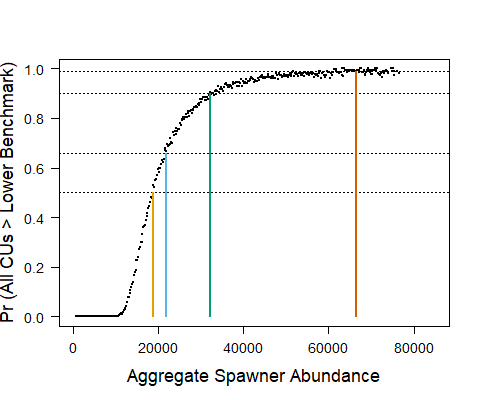
\includegraphics[width=0.6\linewidth]{figure/methods-Example-ProjectedLRP}}{Figure \ref{fig:example-projectedCurve}} 

}

\caption{Example of projected probability curve derived from projections over 30 years and 10,000 MC trials.  The curve shows the projected probability of all CUs being above their lower benchmark (LBM) as a function of aggregate SMU abundance, where aggregate spawning abundance is a bin of 200 fish (e.g., 0-200, 201-400, etc.). Each dot in the curve represents a single combination of year and simulation trial. Coloured lines demonstrate how aggregate abundance LRPs are calculated for 4 different probability thresholds: p* = 0.5 (yellow), 0.66 (blue), 0.90 (green), and 0.99 (orange) for the probability that all CUs are greater than their LBM. Horizontal dotted lines intersect the y-axis at each probability threshold, while the solid vertical lines show the corresponding aggregate escapement that will represent the LRP.}\label{fig:example-projectedCurve}
\end{figure}
\hypertarget{IFCChapter}{%
\section{CASE STUDY 1: INTERIOR FRASER COHO SALMON}\label{IFCChapter}}

\hypertarget{context}{%
\subsection{CONTEXT}\label{context}}

The Interior Fraser Coho Salmon Stock Management Unit (SMU) includes Coho Salmon that return to the Fraser River and tributaries upstream of Hell's Gate in the Fraser Canyon. Like most Coho Salmon, Interior Fraser Coho spend at least one full year in freshwater as fry before migrating to the ocean as smolts (\protect\hyperlink{ref-arbeiderInteriorFraserCoho2020}{Arbeider et al. 2020}). Most (88\%) IFC have a 3-year life history, in which they leave freshwater in their second year and spend 18 months at sea prior to returning to their natal system to spawn. The remaining 12\% have a 4-year life history in which they spend an additional year in freshwater before migrating as smolts in their third year. Both the 3-year and 4-year life histories spend 18 months at sea. Less than 1\% of Interior Fraser Coho are believed to return as jacks (precocious mature males that spend only 6 months as sea) or at ages older than 4 years (\protect\hyperlink{ref-arbeiderInteriorFraserCoho2020}{Arbeider et al. 2020}).

WSP CUs have been identified for Interior Fraser Coho based on genetics and geographic separation: Middle Fraser, Fraser Canyon, Lower Thompson, North Thompson, and South Thompson {[}\protect\hyperlink{ref-dfoWildSalmonPolicy2015}{DFO} (\protect\hyperlink{ref-dfoWildSalmonPolicy2015}{2015}); Figure~\ref{fig:coho-map}{]}. Previous work by the Interior Fraser Coho Recovery Team (IFCRT) identified 11 subpopulations nested within the five CUs, and developed recovery objectives based on maintaining abundance in each of these smaller subpopulation units {[}\protect\hyperlink{ref-ifcrtinteriorfrasercohorecoveryteamConservationStrategyCoho2006}{IFCRT (Interior Fraser Coho Recovery Team)} (\protect\hyperlink{ref-ifcrtinteriorfrasercohorecoveryteamConservationStrategyCoho2006}{2006}); Table~\ref{tab:cohoCU2SP}{]}. The delineation of subpopulations was based on several factors, including the presence of natural barriers, the influence of large lakes on downstream discharge and thermal regimes, observations of spawner aggregations under differing discharge conditions, and genetic differentiation evidence . The 11 subpopulations are described in detail by the \protect\hyperlink{ref-ifcrtinteriorfrasercohorecoveryteamConservationStrategyCoho2006}{IFCRT (Interior Fraser Coho Recovery Team)} (\protect\hyperlink{ref-ifcrtinteriorfrasercohorecoveryteamConservationStrategyCoho2006}{2006}).
\begin{figure}[htb]

{\centering \pdftooltip{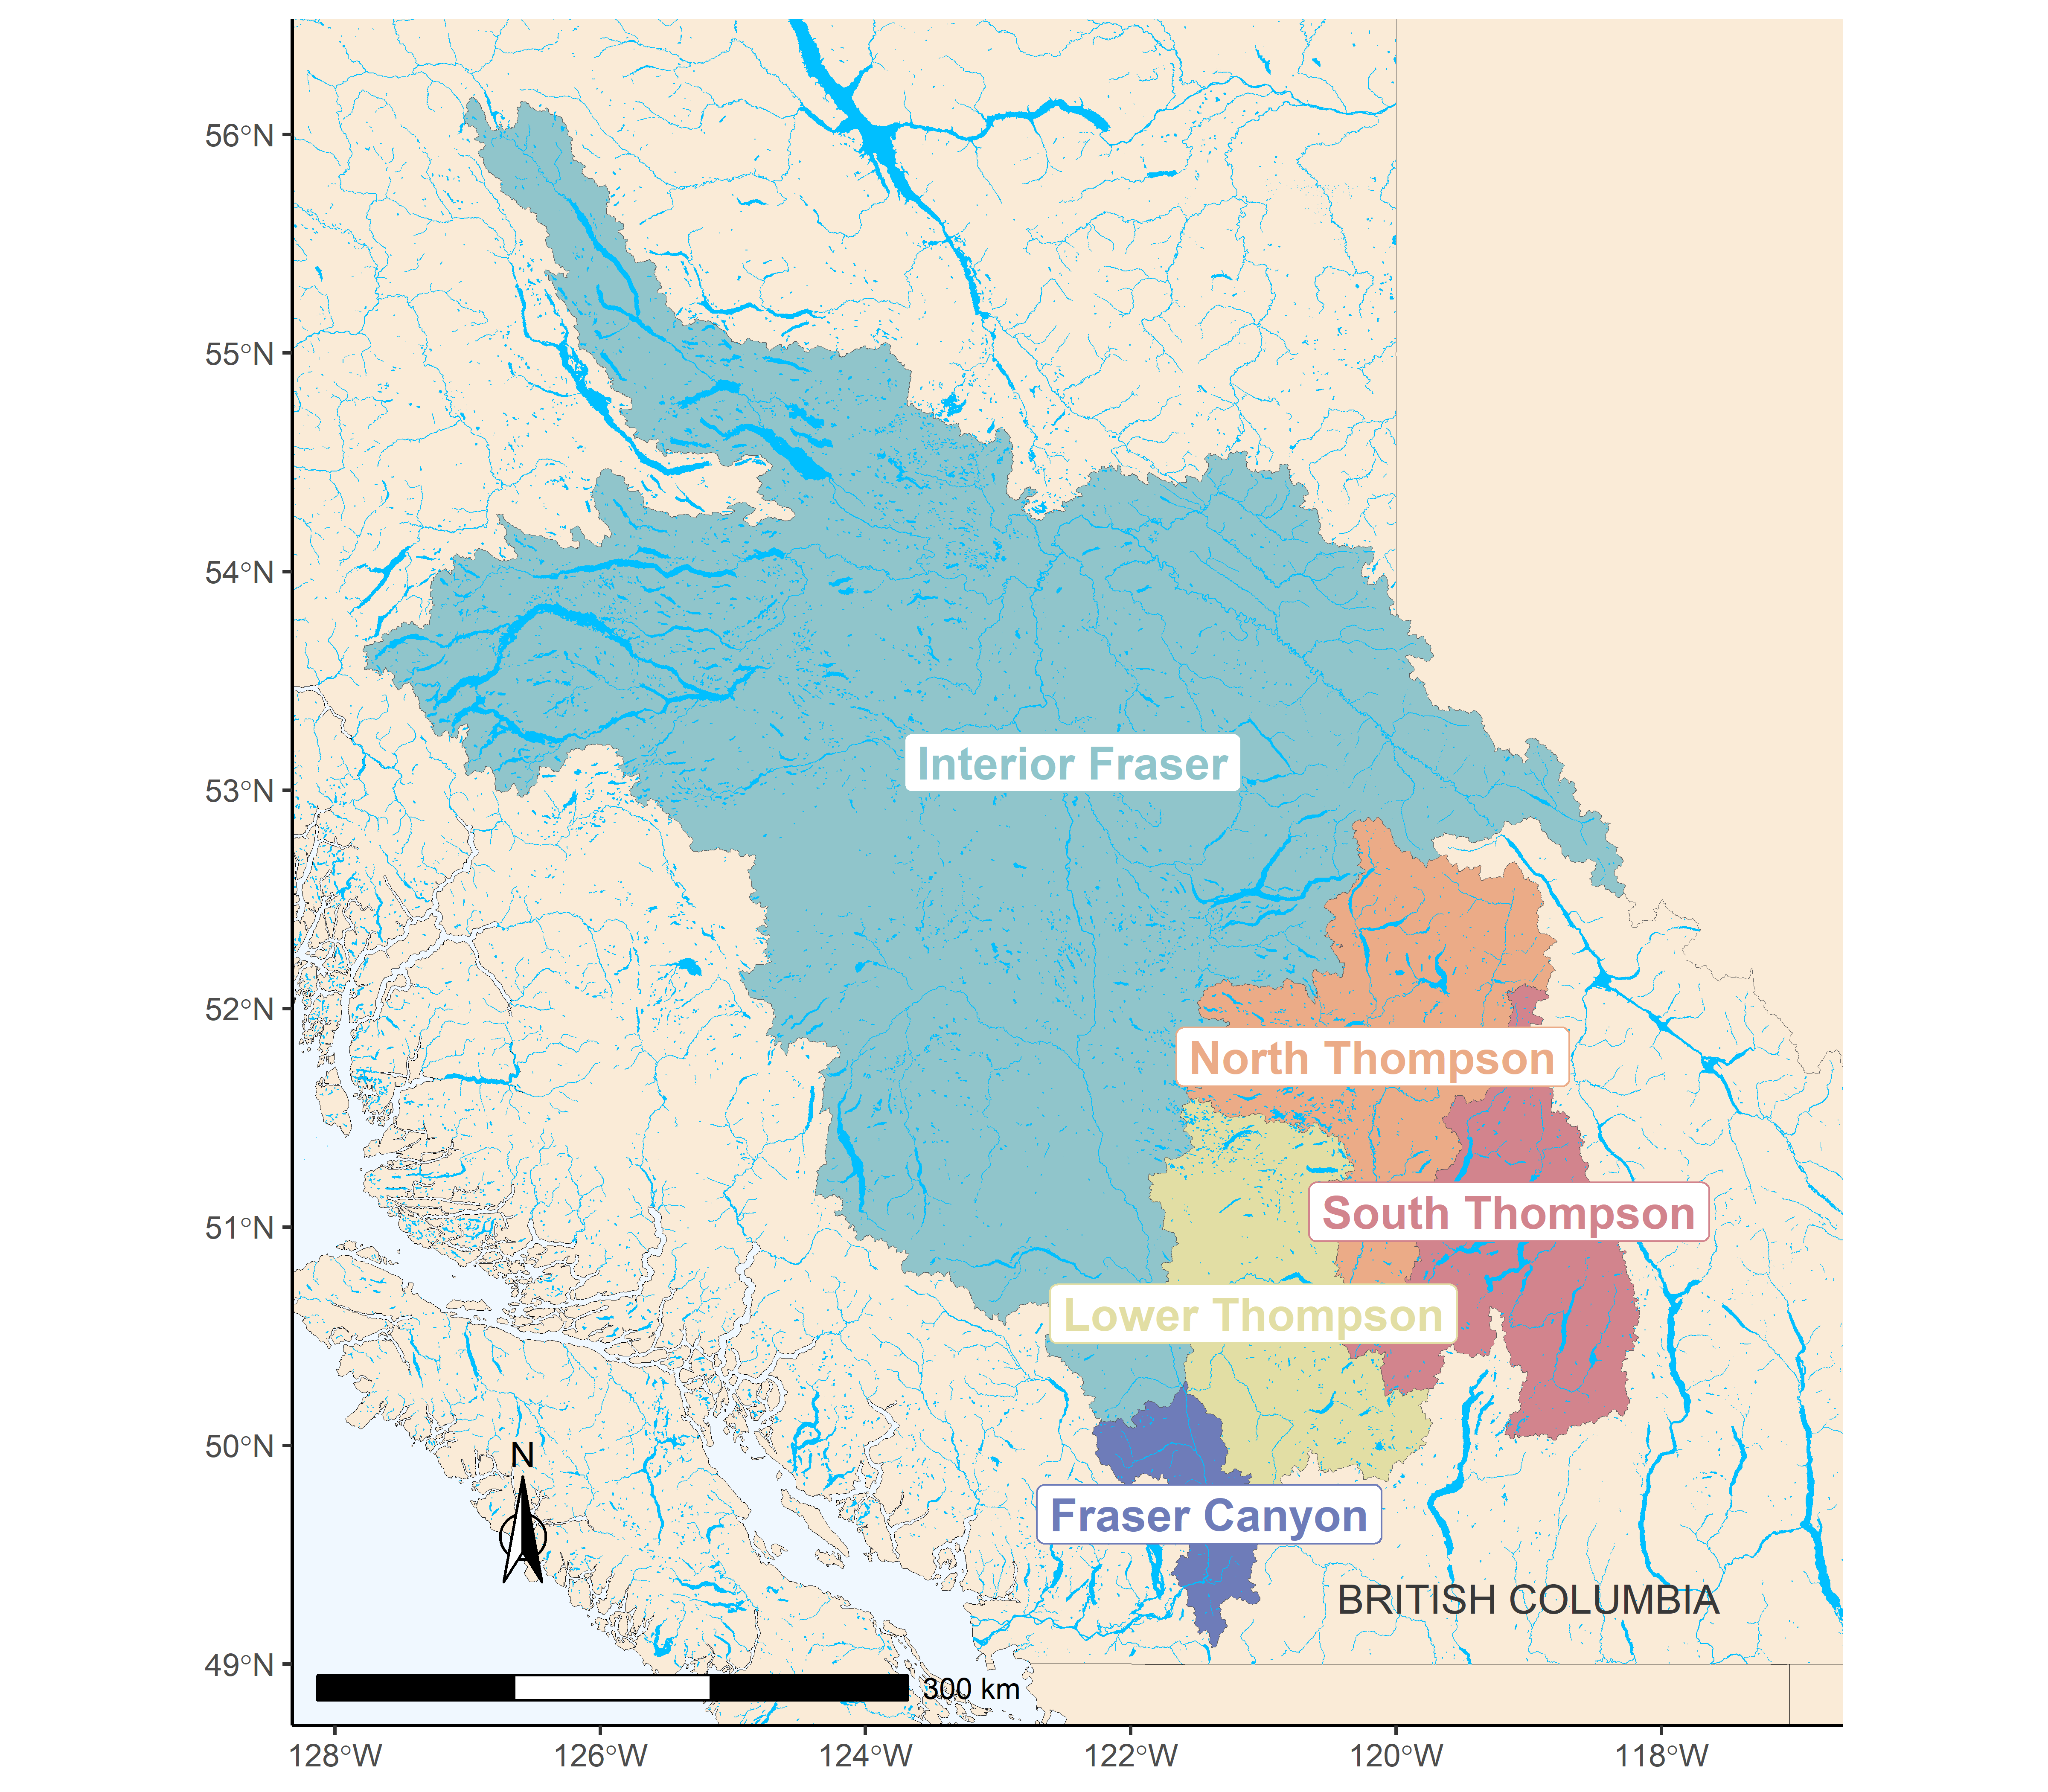
\includegraphics[width=0.6\linewidth]{figure/coho-map}}{Figure \ref{fig:coho-map}} 

}

\caption{The five Conservation Units that make up the Interior Fraser Coho Stock Management Unit.}\label{fig:coho-map}
\end{figure}
\begin{longtable}[]{@{}
  >{\raggedright\arraybackslash}p{(\columnwidth - 2\tabcolsep) * \real{0.28}}
  >{\raggedright\arraybackslash}p{(\columnwidth - 2\tabcolsep) * \real{0.46}}@{}}
\caption{\label{tab:cohoCU2SP} Interior Fraser Coho Conservation Units (CUs) and associated sub-populations. Note that the definition of these sub-populations, including mapped boundaries, are provided in \protect\hyperlink{ref-ifcrtinteriorfrasercohorecoveryteamConservationStrategyCoho2006}{IFCRT (Interior Fraser Coho Recovery Team)} (\protect\hyperlink{ref-ifcrtinteriorfrasercohorecoveryteamConservationStrategyCoho2006}{2006}).}\tabularnewline
\toprule
\begin{minipage}[b]{\linewidth}\raggedright
Conservation Unit
\end{minipage} & \begin{minipage}[b]{\linewidth}\raggedright
Sub-populations
\end{minipage} \\
\midrule
\endfirsthead
\toprule
\begin{minipage}[b]{\linewidth}\raggedright
Conservation Unit
\end{minipage} & \begin{minipage}[b]{\linewidth}\raggedright
Sub-populations
\end{minipage} \\
\midrule
\endhead
Middle Fraser & \begin{minipage}[t]{\linewidth}\raggedright
\begin{itemize}

\item
  Lower Middle Fraser
\item
  Upper Middle Fraser
\end{itemize}
\end{minipage} \\
Fraser Canyon & \begin{minipage}[t]{\linewidth}\raggedright
\begin{itemize}

\item
  Nahatlatch
\end{itemize}
\end{minipage} \\
Lower Thompson & \begin{minipage}[t]{\linewidth}\raggedright
\begin{itemize}

\item
  Lower Thompson
\item
  Nicola
\end{itemize}
\end{minipage} \\
North Thompson & \begin{minipage}[t]{\linewidth}\raggedright
\begin{itemize}

\item
  Lower North Thompson
\item
  Middle Thompson
\item
  Upper North Thompson
\end{itemize}
\end{minipage} \\
South Thompson & \begin{minipage}[t]{\linewidth}\raggedright
\begin{itemize}

\item
  Adams Drainage
\item
  Lower and Middle Shuswap Rivers
\item
  Shuswap Lake Tributaries
\end{itemize}
\end{minipage} \\
\bottomrule
\end{longtable}
\hypertarget{previous-assessments}{%
\subsubsection{Previous assessments}\label{previous-assessments}}

Declines in Interior Fraser Coho spawner abundance throughout the 1990's led to a suite of management actions to promote recovery, including significant fishery restrictions starting in 1998 (\protect\hyperlink{ref-deckerAssessmentInteriorFraser2014}{Decker et al. 2014}). Evidence of a new, lower productivity regime starting in return year 1994 that coincides with declines in spawner abundances has been well documented (\protect\hyperlink{ref-deckerAssessmentInteriorFraser2014}{Decker et al. 2014}). In 2002, the Interior Fraser Coho stock management unit was designated `endangered; by the Committee on the Status of Endangered Wildlife in Canada (COSEWIC) based on the stock unit being assessed as a single 'Designatable Unit' (DU). Subsequent work by the Interior Fraser Coho Recovery Team (IFCRT) lead to a conservation strategy outlining short-term and long-term recovery objectives for the management unit (\protect\hyperlink{ref-ifcrtinteriorfrasercohorecoveryteamConservationStrategyCoho2006}{IFCRT (Interior Fraser Coho Recovery Team) 2006}). In 2014, \protect\hyperlink{ref-deckerAssessmentInteriorFraser2014}{Decker et al.} (\protect\hyperlink{ref-deckerAssessmentInteriorFraser2014}{2014}) assessed status relative to the 2006 IFCRT objectives, and concluded that Interior Fraser Coho had been above the short-term recovery target of in every year since 2008, and above the long-term recovery target in the most recent two return years (2012 and 2013). Also in 2014, Interior Fraser Coho were assessed under the framework of DFO's Wild Salmon Policy (WSP). The WSP Integrated Status Assessment classified three of these CUs as being amber status (Middle Fraser, Fraser Canyon, South Thompson) and the remaining two CUs as amber/green status (Lower Thompson, North Thompson; (\protect\hyperlink{ref-dfoWildSalmonPolicy2015}{DFO 2015})). As part of the WSP assessment, \(S_{gen}\) was estimated for each CU and used as one of several benchmarks considered when assigning integrated CU status. A subsequent COSEWIC assessment in 2016 upgraded the status designation for the Interior Fraser Coho DU from `endangered' to `threatened' (\protect\hyperlink{ref-cosewicCOSEWICAssessmentStatus2016}{COSEWIC 2016}). In 2018, DFO undertook a Recovery Potential Assessment (RPA) for Interior Fraser Coho that described status, habitat, threats, limiting factors to recovery, candidate recovery targets, and abundance projections for the DU, as well as recommendations regarding mitigation and allowable harm (\protect\hyperlink{ref-arbeiderInteriorFraserCoho2020}{Arbeider et al. 2020}).

\hypertarget{history-of-aggregate-abundance-based-reference-points}{%
\subsubsection{History of aggregate-abundance based reference points}\label{history-of-aggregate-abundance-based-reference-points}}

Interior Fraser Coho show a strong positive relationship between their spatial distribution and overall abundance, which has been used as a basis for identifying aggregate abundance-based recovery targets and reference points for the stock group. Starting in 2006, the IFCRT identified a recovery goal of one or more viable sub-populations in each of the five `populations,' where their definition of populations aligns with CUs under the WSP (\protect\hyperlink{ref-ifcrtinteriorfrasercohorecoveryteamConservationStrategyCoho2006}{IFCRT (Interior Fraser Coho Recovery Team) 2006}); note that from this point on, we use the term CU instead of population when describing IFCRT recovery goals to be consistent with the WSP). The IFCRT identified a short-term recovery objective that the 3-year average escapement in at least half of the sub-populations within each of the five CUs was to exceed 1,000 wild-origin spawning Coho Salmon, excluding hatchery fish spawning in the wild. Based on analysis of the relationship between aggregate abundance and the number of CUs that met this objective based on historical data, the IFCRT identified an abundance-based short-term recovery target of 20,000 spawners as the level required to meet their distributional objective. In addition, the IFCRT identified a long-term recovery target of 40,000 spawners, which represented a level that was expected to maintain 1,000 or more wild Coho Salmon in all 11 sub-populations. \protect\hyperlink{ref-deckerAssessmentInteriorFraser2014}{Decker et al.} (\protect\hyperlink{ref-deckerAssessmentInteriorFraser2014}{2014}) updated the IFCRT's original analysis using a longer time series of escapement data. They also quantified the relationship between aggregate abundance and distribution by using a logistic regression to estimate the probability of meeting short-term and long-term recovery objectives as a function of aggregate abundance. The concluded that aggregate spawner abundance levels of 20,000 and 40,000 spawners would result in near 100\% probability that the IFCRT's short-term objective and long-term recovery objectives would be met, respectively. \protect\hyperlink{ref-kormanEvaluationFrameworkAssessing2019}{Korman et al.} (\protect\hyperlink{ref-kormanEvaluationFrameworkAssessing2019}{2019}) also used logistic regressions of the relationship between the IFCRT's distributional objectives and aggregate abundance when evaluating how exploitation and marine survival rates affected the ability of Interior Fraser Coho to meet conservation targets. Their approach was similar to that of \protect\hyperlink{ref-deckerAssessmentInteriorFraser2014}{Decker et al.} (\protect\hyperlink{ref-deckerAssessmentInteriorFraser2014}{2014}), except they applied logistic regressions at the CU-level instead of the SMU-level. Using this approach, they calculated the probability that IFCRT sub-population objectives were met as a function of total escapement to the CU within their simulation evaluation. When evaluating how well conservation targets were met at the MU-level, they chose to rely on the previous values of 20,000 and 40,000 identified by the IFCRT instead of updating these values. Finally, the 2018 RPA used an updated logistic regression to identify a long-term recovery target for Interior Fraser Coho that met the long-term IFCRT objective of 1000 spawners in all sub-populations (\protect\hyperlink{ref-arbeiderInteriorFraserCoho2020}{Arbeider et al. 2020}). As a result, \protect\hyperlink{ref-arbeiderInteriorFraserCoho2020}{Arbeider et al.} (\protect\hyperlink{ref-arbeiderInteriorFraserCoho2020}{2020}) recommended that the long-term recovery target for the stock should be a 3-year geometric mean abundance of 35,935 natural-origin spawners.

\hypertarget{cohoData}{%
\subsection{DATA}\label{cohoData}}

Data for this case study cover return years 1998 -2020. Data prior to 1998 were not used due to concerns about inconsistent assessment methods and data quality. All Interior Fraser Coho data were provided by DFO's Fraser River Stock Assessment Unit (M. Arbeider, pers. comm). These data included: (i) annual spawner abundance by CU (1998-2020), (ii) annual recruits-at-age by CU (brood years 1998 - 2016), (iii) a hatchery-based smolt-to-adult survival rate index, (iv) annual exploitation rates, and (v) annual spawner abundances for 11 sub-populations nested within the 5 CUs. Data were similar to those previously described in \protect\hyperlink{ref-arbeiderInteriorFraserCoho2020}{Arbeider et al.} (\protect\hyperlink{ref-arbeiderInteriorFraserCoho2020}{2020}); data treatments, assumptions, infilling, and data quality are described in detail in that document. More recent updates that are not described in \protect\hyperlink{ref-arbeiderInteriorFraserCoho2020}{Arbeider et al.} (\protect\hyperlink{ref-arbeiderInteriorFraserCoho2020}{2020}) include the incorporation of three additional years of data (return years 2018-2020; brood years 2014-2016), updates to the smolt-to-adult marine survival rate index to use a weighted average by release size, and increased data quality screening of scale ages used to calculate the proportion of recruits at age (M. Arbeider, pers. comm).

The exploitation rate time series is a large source of uncertainty for Interior Fraser Coho. Exploitation rates are only available at the SMU-level, so are assumed constant among all CUs, which is unlikely to be true. Furthermore, models used to reconstruct exploitation rates require a large number of assumptions that are expected to be incorrect (\protect\hyperlink{ref-arbeiderInteriorFraserCoho2020}{Arbeider et al. 2020}). Because exploitation rate time series are used to reconstruct spawner-recruit time series, errors in exploitation rates will propagate through to estimates of stock recruitment parameters, relative abundance-based benchmarks such as \(S_{gen}\), and covaration in recruitment residuals. Additional sources of uncertainty in Interior Fraser Coho data sets include observation errors in spawner abundance estimates and estimates of age-at-maturity. Spawner abundance estimates are largely derived from visual surveys. Scale sampling to determine age structure is incomplete at the CU-level with small sample sizes, missing data, and limited spatial representation within CUs in some years (\protect\hyperlink{ref-kormanEvaluationFrameworkAssessing2019}{Korman et al. 2019})

\hypertarget{cu-status-estimation}{%
\subsection{CU STATUS ESTIMATION}\label{cu-status-estimation}}

We use three alternative ways to characterize CU status when developing LRPs for Interior Fraser Coho: 1) Rapid multi-dimensional scanner tool, 2) CU-level abundance relative to \(S_{gen}\) as a lower benchmark on abundance, and 3) Distribution of spawning abundance relative to distributional targets developed by the IFCRT.

The first approach, which uses the rapid multidimensional scanning tool developed by the State of the Salmon program (Section~\ref{rapidToolMethods}), is consistent with Canada's WSP and is recommended by Holt et al.~(in review) as the method that should be used to estimate CU status when using the proportional LRP approach. The other two approaches are primarily used to develop aggregate abundance-based LRPs in this case study, as well as for a point of comparison with the rapid multidimensional scanning tool.

The second approach is based on comparing the current abundance of each CU to its CU-specific estimate of \(S_{gen}\), where CU status is considered poor when abundance drops below \(S_{gen}\). The value of \(S_{gen}\) represents the number of spawners required to recover to \(S_{MSY}\) (spawners maximum sustainable yield) within one generation, under equilibrium conditions in the absence of fishing (\protect\hyperlink{ref-holtIndicatorsStatusBenchmarks2009}{Holt et al. 2009}). \(S_{gen}\) is one of several benchmarks available for assigning multidimensional CU status in WSP Integrated Status Assessments; it represents a lower benchmark between red and amber status zones and was used as part of the 2014 Integrated Status Assessment for Interior Fraser Coho (\protect\hyperlink{ref-dfoWildSalmonPolicy2015}{DFO 2015}).

The third approach is based on the distribution of spawning escapement among subpopulations nested within CUs (Table~\ref{tab:cohoCU2SP}). We apply this approach for Interior Fraser Coho to maintain consistency with previous recovery planning processes for this SMU (\protect\hyperlink{ref-ifcrtinteriorfrasercohorecoveryteamConservationStrategyCoho2006}{IFCRT (Interior Fraser Coho Recovery Team) 2006}; \protect\hyperlink{ref-arbeiderInteriorFraserCoho2020}{Arbeider et al. 2020}). Since the distributional target we use was initially developed by the Interior Fraser Coho Recovery Team in 2006, we refer to it as ``IFCRT distributional.'' Specifically, we use the IFCRT's short-term recovery objective that the 3-year average escapement in at least half of the sub-populations within each of the five CUs is to exceed 1,000 wild-origin spawning Coho salmon, excluding hatchery fish spawning in the wild. We selected the short-term recovery target to represent poor CU status in our case study (e.g., below a lower benchmark) because, as noted by \protect\hyperlink{ref-arbeiderInteriorFraserCoho2020}{Arbeider et al.} (\protect\hyperlink{ref-arbeiderInteriorFraserCoho2020}{2020}), the short-term target was designed as an immediate target when the population was endangered. As such, it was interpreted as a level expected to prevent extinction or loss of genetic diversity. We have included this third approach to defining CU status to demonstrate the range of approaches and metrics that can be used, and to demonstrate sensitivity of the LRP to choice of metrics for assigning CU-status. Future iterations of the multidimensional approach could include distributional metrics such as those used in the IFCRT approach.

\hypertarget{cohoSgen}{%
\subsubsection{Estimation of Sgen}\label{cohoSgen}}

Estimates of Sgen are required when assessing CU status using both the `Rapid Multidimensional Scanning Tool' and the comparison of current CU-level abundance to \(S_{gen}\). Two different formulations of stock recruitment model were used to estimate \(S_{gen}\): (i) a base Ricker model, which includes a marine survival covariate, and (ii) a Ricker\_prioCap model in which an informative prior distribution is used to increase \(S_{REP}\) compared to the base model. \(S_{REP}\) is the spawner abundance level at which the stock replaces itself; the relationship between \(S_{REP}\) and Ricker stock recruit model parameters is shown below. Both of these models have been previously developed and applied to Interior Fraser Coho CUs. The marine survival covariate used when fitting both models is a hatchery-based smolt-to-adult survival rate index. The index is not CU-specific; the same index is applied to all CUs. A third Ricker model, in which both an informative prior on \(S_{REP}\) and depensatory mortality were included, was also used by \protect\hyperlink{ref-kormanEvaluationFrameworkAssessing2019}{Korman et al.} (\protect\hyperlink{ref-kormanEvaluationFrameworkAssessing2019}{2019}) and \protect\hyperlink{ref-arbeiderInteriorFraserCoho2020}{Arbeider et al.} (\protect\hyperlink{ref-arbeiderInteriorFraserCoho2020}{2020}); however, we did not include it in our case study for simplicity. As noted by \protect\hyperlink{ref-kormanEvaluationFrameworkAssessing2019}{Korman et al.} (\protect\hyperlink{ref-kormanEvaluationFrameworkAssessing2019}{2019}), there is no indication in available data of depensatory dynamics, and the SR model fit with depensatory mortality required a highly uncertain assumption to be made about the escapement level at which recruitment is reduced to 50\% of the value it would have been in the absence of depensatory mortality. Furthermore, formal model selection criteria showed that adding depensatory mortality into models lead to a reduction in model fit (\protect\hyperlink{ref-kormanEvaluationFrameworkAssessing2019}{Korman et al. 2019}).

\protect\hyperlink{ref-kormanEvaluationFrameworkAssessing2019}{Korman et al.} (\protect\hyperlink{ref-kormanEvaluationFrameworkAssessing2019}{2019}) and \protect\hyperlink{ref-arbeiderInteriorFraserCoho2020}{Arbeider et al.} (\protect\hyperlink{ref-arbeiderInteriorFraserCoho2020}{2020}) used a hierarchical model structure for both the base Ricker and Ricker\_priorCap models that assumed CU-level productivity parameters were sampled from a common, normal distribution shared by all CUs. Using formal model selection criteria (i.e., DIC), \protect\hyperlink{ref-kormanEvaluationFrameworkAssessing2019}{Korman et al.} (\protect\hyperlink{ref-kormanEvaluationFrameworkAssessing2019}{2019}) found higher support for the hierarchical structure than when productivity parameters were assumed independent among CUs. However, our initial examination of the hierarchical approach applied to the updated data set lead us to select the independent CU approach for our evaluation. Firstly, we found that LRP estimates were sensitive to the assumed standard deviation on the hyper-distribution prior for the productivity parameter. Using the individual model approach removed prior influence on model results. Secondly, a logistic regression fit to status estimates obtained using the hierarchical model was unable to converge on a solution in several years between 2015 and 2020, including the most recent year (2020). Thirdly, because all CUs had equal amounts of data, the commonly cited benefit of hierarchical models allowing data-poor systems to borrow information from data-rich systems did not apply. While future stock recruit analyses for Interior Fraser Coho may wish to re-visit the hierarchical approach to modelling intrinsic productivity, we do not expect our decision to apply an individual modelling approach here will affect out general conclusions.

The formulations for our two stock recruitment models using the assumption of independent productivity among CUs are described below.

\emph{Model 1: Ricker}

The base Ricker stock recruit model formulation was:
\begin{equation}
  R_{i,a,t} = P_{i,a,t-a}S_{i,t-a}e^{log(\alpha_i) + \gamma log(m_{t-1})-\beta_i S_{i,t-a}e^{v_i}-\sigma^2/2}
   \label{eq:rickerSurv-IM}
\end{equation} \begin{equation}
  v_i \sim Normal(0,\sigma_{v_i})
\end{equation}
where,

\(R_{i,a,t}\) = the predicted number of natural origin recruits from CU \(i\) of age \(a\) returning in year \(t\) (i.e., recruits that were produced by escapement in brood year \(t-a\))

\(P_{i,a,t-a}\) = the proportion of recruitment from CU \(i\) returning at age \(a\) from brood year \(t-a\)

\(S_{i,t-a}\) = spawners from CU \(i\) in brood year \(t-a\)

\(\alpha_i\) = productivity parameter for CU \(i\)

\(\gamma\) = marine survival co-efficient shared among CUs

\(m_{t-1}\) = hatchery marine survival index (smolt-to-adult) shared among CUs for sea entry in year t-1

\(\beta_i\) = density dependent term describing the rate of decrease in log-survival for CU \(i\) with increasing spawner abundance

\(\sigma_{v_i}\) = standard deviation of process error on recruitment deviations

This model formulation is similar to the Ricker model used in \protect\hyperlink{ref-arbeiderInteriorFraserCoho2020}{Arbeider et al.} (\protect\hyperlink{ref-arbeiderInteriorFraserCoho2020}{2020}), but without a hierarchical structure imposed on \(log(\alpha_i)\). We placed the following non-informative constraints on the likelihood function to replicate the Bayesian model fitting routine of \protect\hyperlink{ref-arbeiderInteriorFraserCoho2020}{Arbeider et al.} (\protect\hyperlink{ref-arbeiderInteriorFraserCoho2020}{2020}):
\begin{equation}
  \gamma \sim Normal(0,10)
\end{equation} \begin{equation}
  \sigma_{v_i} \sim Inverse Gamma (0.1,0.1)
\end{equation}
\emph{Model 2: Ricker\_priorCap}

To maintain consistency with this previous work on Interior Fraser Coho, we also consider a version of the Ricker model that uses an informative prior distribution on \(S_{REP}\) to increase carrying capacity. \protect\hyperlink{ref-kormanEvaluationFrameworkAssessing2019}{Korman et al.} (\protect\hyperlink{ref-kormanEvaluationFrameworkAssessing2019}{2019}) suggested that the Ricker model with a survival co-variate (Model 1) over-estimated compensatory dynamics at high spawner abundances when applied only to data from 1998 onwards. They noted that spawner abundances since 1998 have been much lower than historic levels. Given that sparse data at high spawner abundances makes it difficult to estimate carrying capacity, base Ricker estimates of carrying capacity may be unreliable (\protect\hyperlink{ref-kormanEvaluationFrameworkAssessing2019}{Korman et al. 2019}). Furthermore, they observed that one brood line had persisted at a relatively higher and more stable spawner abundance than the other two brood lines, which they viewed as evidence for a higher capacity than the base Ricker model estimates. Based on these concerns, \protect\hyperlink{ref-kormanEvaluationFrameworkAssessing2019}{Korman et al.} (\protect\hyperlink{ref-kormanEvaluationFrameworkAssessing2019}{2019}) proposed an alternative Ricker model that used an informative prior distribution to increase carrying capacity (represented as the spawner abundance at which the stock replaces itself, \(S_{REP}\)). \protect\hyperlink{ref-arbeiderInteriorFraserCoho2020}{Arbeider et al.} (\protect\hyperlink{ref-arbeiderInteriorFraserCoho2020}{2020}) followed the approach of \protect\hyperlink{ref-kormanEvaluationFrameworkAssessing2019}{Korman et al.} (\protect\hyperlink{ref-kormanEvaluationFrameworkAssessing2019}{2019}) by considering both the base Ricker model and a version of the Ricker model with an informative prior distribution on \(S_{REP}\) to be plausible when providing management advice.
\begin{equation}
  \beta_i = \frac{\alpha_i + \gamma + log(\overline{m})}{S_{REP,i}}
   \label{eq:beta-Srep}
\end{equation} \begin{equation}
  S_{REP,i} \sim Normal(\mu_{SREP},\sigma_{SREP})
\end{equation}
\protect\hyperlink{ref-arbeiderInteriorFraserCoho2020}{Arbeider et al.} (\protect\hyperlink{ref-arbeiderInteriorFraserCoho2020}{2020}) and \protect\hyperlink{ref-kormanEvaluationFrameworkAssessing2019}{Korman et al.} (\protect\hyperlink{ref-kormanEvaluationFrameworkAssessing2019}{2019}) set \(\mu_{SREP}\) at 1.5 times the \(S_{REP}\) value estimated from the base model fit without a prior on \(S_{REP}\). For our integrated Sgen-LRP model fits (described in section xxx) , we found that we needed to constrain \(\mu_{SREP}\) at no more than 1.4 times the \(S_{REP}\) value to achieve model convergence, so we used the 1.4 times expansion instead. We set \(\sigma_{SREP}\) at \(\sqrt{2} * 1000 = 1414\) spawners, which is the same value used by \protect\hyperlink{ref-arbeiderInteriorFraserCoho2020}{Arbeider et al.} (\protect\hyperlink{ref-arbeiderInteriorFraserCoho2020}{2020}). Note that the ``\(* 1000\)'' term is used to correct for scaling spawner abundance by 1/1000 when fitting models. \protect\hyperlink{ref-arbeiderInteriorFraserCoho2020}{Arbeider et al.} (\protect\hyperlink{ref-arbeiderInteriorFraserCoho2020}{2020}) parameterized the distribution in terms of precision (\(\tau\)), where \(\tau = \frac{1}{\sigma^2} = 0.5\). The effect of adding the prior on \(S_{REP}\) when fitting individual models to available data is shown in Figure~\ref{fig:coho-SR-fit}.
\begin{figure}[htb]

{\centering \pdftooltip{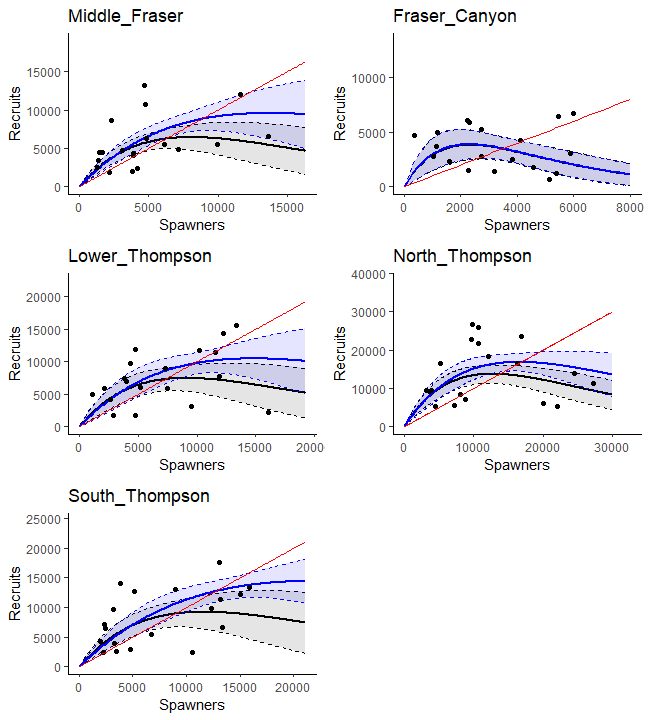
\includegraphics[width=6in]{figure/coho-compare-SRFits-IM}}{Figure \ref{fig:coho-SR-fit}} 

}

\caption{Spawner-recruitment curves fit to spawner and recruitment data using individual models for each CU. Solid black lines shows the MLE fit for the base Ricker model while solid blue lines shows the MLE fit for the Ricker\_priorCap model.  Associated black and blue shaded regions show the 95 percent confidence intervals on respective model fits. The red line show the replacement line.}\label{fig:coho-SR-fit}
\end{figure}
\emph{Calculation of Sgen}

The inclusion of a marine survival co-variate in all four spawner recuit models means that the realized productivity changes from year to year with changing marine survival. We incorporated this adjustment into our calculations of \(S_{gen}\) by first calculating the effective productivity for each CU as:
\begin{equation}
  log(\alpha'_{i}) = log(\alpha_i) + \gamma log(\overline{m})
   \label{eq:adjProd}
\end{equation}
where, \(\overline{m}\) is the average marine survival rate over the available time series.

\(S_{MSY}\) was calculated as a function of log(\(\alpha_i'\)) and \(\beta_i\) using:
\begin{equation}
  S_{MSY,i} = 1 - \frac{W(e^1-\alpha'_i)}{\beta_i} 
   \label{eq:Smsy}
\end{equation}
where, \(W\) represents the Lambert W function (\protect\hyperlink{ref-scheuerellExplicitSolutionCalculating2016}{Scheuerell 2016}). \(S_{gen}\) was then calculated numerically by solving the following equation:
\begin{equation}
  S_{MSY,i} = S_{gen,i}e^(log(\alpha'_{i})- \beta_i \cdot S_{gen})
  \label{eq:Sgen}
\end{equation}
\hypertarget{lrp-estimation-proportion-of-cus}{%
\subsection{LRP ESTIMATION: PROPORTION OF CUS}\label{lrp-estimation-proportion-of-cus}}

\hypertarget{methods}{%
\subsubsection{Methods}\label{methods}}

We looked at the proportion of CUs that had rapid multidimensional status assessments above the red zone to determine in which years between 1998 and 2020 the LRP would have been breached. Status was assessed as being below the LRP in years in which one or more CUs assessed as having red status. Both Ricker model formulations described above were used to estimate relative abundance-based benchmarks (lower benchmark = \(S_{gen}\) and upper benchmark = 0.8\(S_{MSY}\)) when assessing multi-dimensional rapid status: the base Ricker model and the Ricker\_priorCap model. Estimates of \(S_{gen}\) and \(S_{MSY}\) were made using all data available up to 2020.

For comparison, we also looked at the proportion of CUs that had recent generational average (3-year) spawning abundance greater than \(S_{gen}\) in each historical year and the proportion of CUs that failed to meet the IFCRT distributional target of at least half of all sub-populations within each CU having more than 1000 spawners.

\hypertarget{results}{%
\subsubsection{Results}\label{results}}

Estimates of \(S_{gen}\) based on the Ricker\_priorCap model were higher than those based on the base Ricker model for four of the five CUs (Middle Fraser, Lower Thompson, North Thompson, and South Thompson) and were approximately equal for the fifth CU (Fraser Canyon; Appendix~\ref{app:coho-appendix} . As a result, generational average spawning abundance was more likely to drop below \(S_{gen}\) when it was estimated using the Ricker\_priorCap. Under the base Ricker model formulation, generational average spawning abundance remained above \(S_{gen}\) for all years between 2000 and 2020 (Figure~\ref{fig:coho-CU-multiDim-Ricker}). In comparison, under the Ricker\_priorCap formulation, generational average abundance dropped below \(S_{gen}\) in one or more years for Lower Thompson CU (2006), Middle Fraser CU (2006, 2008), and South Thompson CU (2000, 2006, 2007, 2015; Figure~\ref{fig:coho-CU-multiDim-Ricker-Cap}). As a result, at least one CU had stock status assessed as below \(S_{gen}\) for 5 of the 21 years between 2000 and 2020.

When CU status was assessed using the multidimensional scanning tool with lower and upper abundance-based benchmarks based on \(S_{gen}\) and 0.8\(S_{MSY}\) as inputs, CU status was always assessed as red for years in which the generational average spawning abundance dropped below \(S_{gen}\), regardless of which stock recruit model was used to estimate benchmarks (Figures~\ref{fig:coho-CU-multiDim-Ricker} and~\ref{fig:coho-CU-multiDim-Ricker-Cap}). This result occurs because according to the multidimensional decision tree (Figure~\ref{fig:decision-tree}), status is derived from abundance-based benchmarks in most years, which means that being below \(S_{gen}\) is most often the trigger for a red CU status assessment. An exception occurs in the Fraser Canyon CU in years 2015-2017. In these years, the generational average of absolute spawning abundance is \textless{} 1500 spawners and CU is assigned red status under the first node of the decision tree even though spawning abundances are above \(S_{gen}\) (Figure~\ref{fig:decision-tree}). As a result, when multidimensional status was assessed using abundance-based benchmarks estimated from the base Ricker model, a proportion-based LRP for the SMU would have been breached in 4 of 21 years based on Fraser Canyon spawning abundances dropping below 1500 spawners in three years (2015-2017), and one year (2000) in which the Lower Thompson CU had spawning abundance \textless{} \(S_{gen}\) (Figure~\ref{fig:coho-CU-multiDim-Ricker}). When multidimensional status was assessed using abundance-based benchmarks from the Ricker\_priorCap model, a proportion-based LRP would have been breached in 9 of 21 years (2000-2001, 2005-2007, 2010, 2015-2017) based on a combination of spawning abundances \textless{} 1500 in the Fraser Canyon CU and spawning abundances \textless{} \(S_{gen}\) in other CUs (Figure~\ref{fig:coho-CU-multiDim-Ricker-Cap}). Multidimensional status based on the rapid screening tool was above red for all CUs in the most recent year, 2020, indicating that the SMU is currently above a proportion-based LRP.
\begin{figure}[htb]

{\centering \pdftooltip{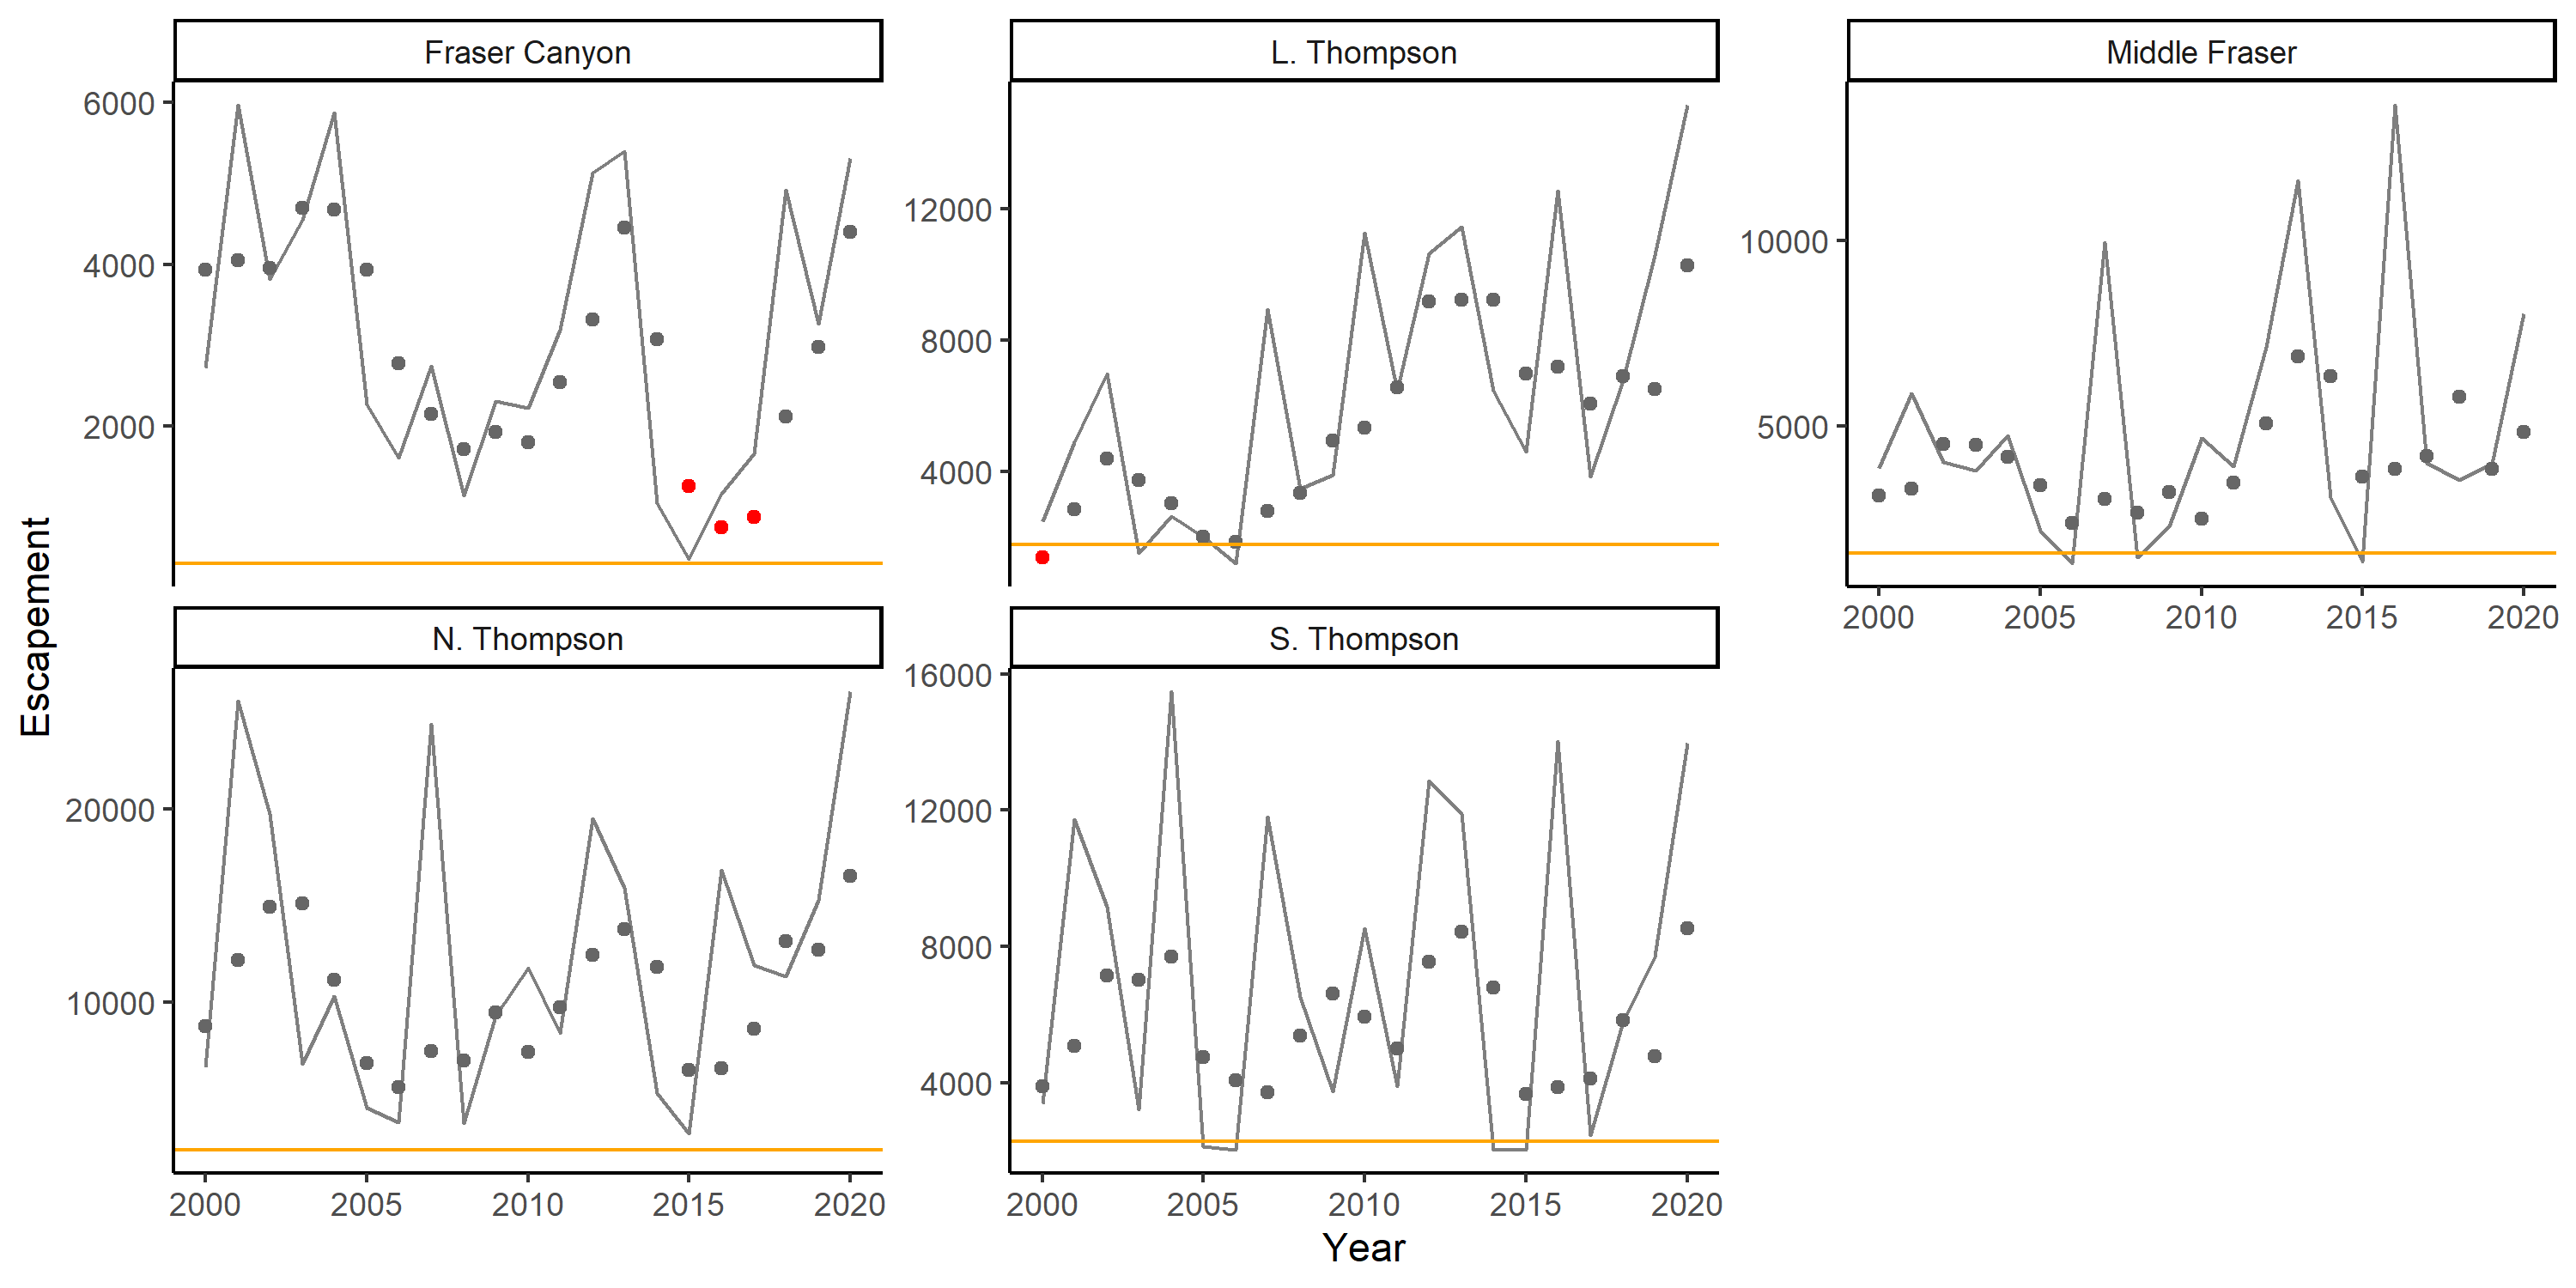
\includegraphics[width=6in]{figure/coho-CU-EscpSeries-wMultiStatus-Ricker}}{Figure \ref{fig:coho-CU-multiDim-Ricker}} 

}

\caption{Escapement time series for five Interior Fraser Coho CUs shown as annual escapements (lines) and 3-year geometric mean escapements (dots). First geometric mean includes years 2008-2000. Grey dots indicate years in which all CUs had multidimensional rapid status assessments above red when Sgen was estimated using the Ricker model, while red dots indicate years in which one or more CUs had multi-dimensional status assessments in the red zone, which would trigger a breach of the LRP. Solid orange lines show estimates of Sgen from the Ricker model for comparison.}\label{fig:coho-CU-multiDim-Ricker}
\end{figure}
\begin{figure}[htb]

{\centering \pdftooltip{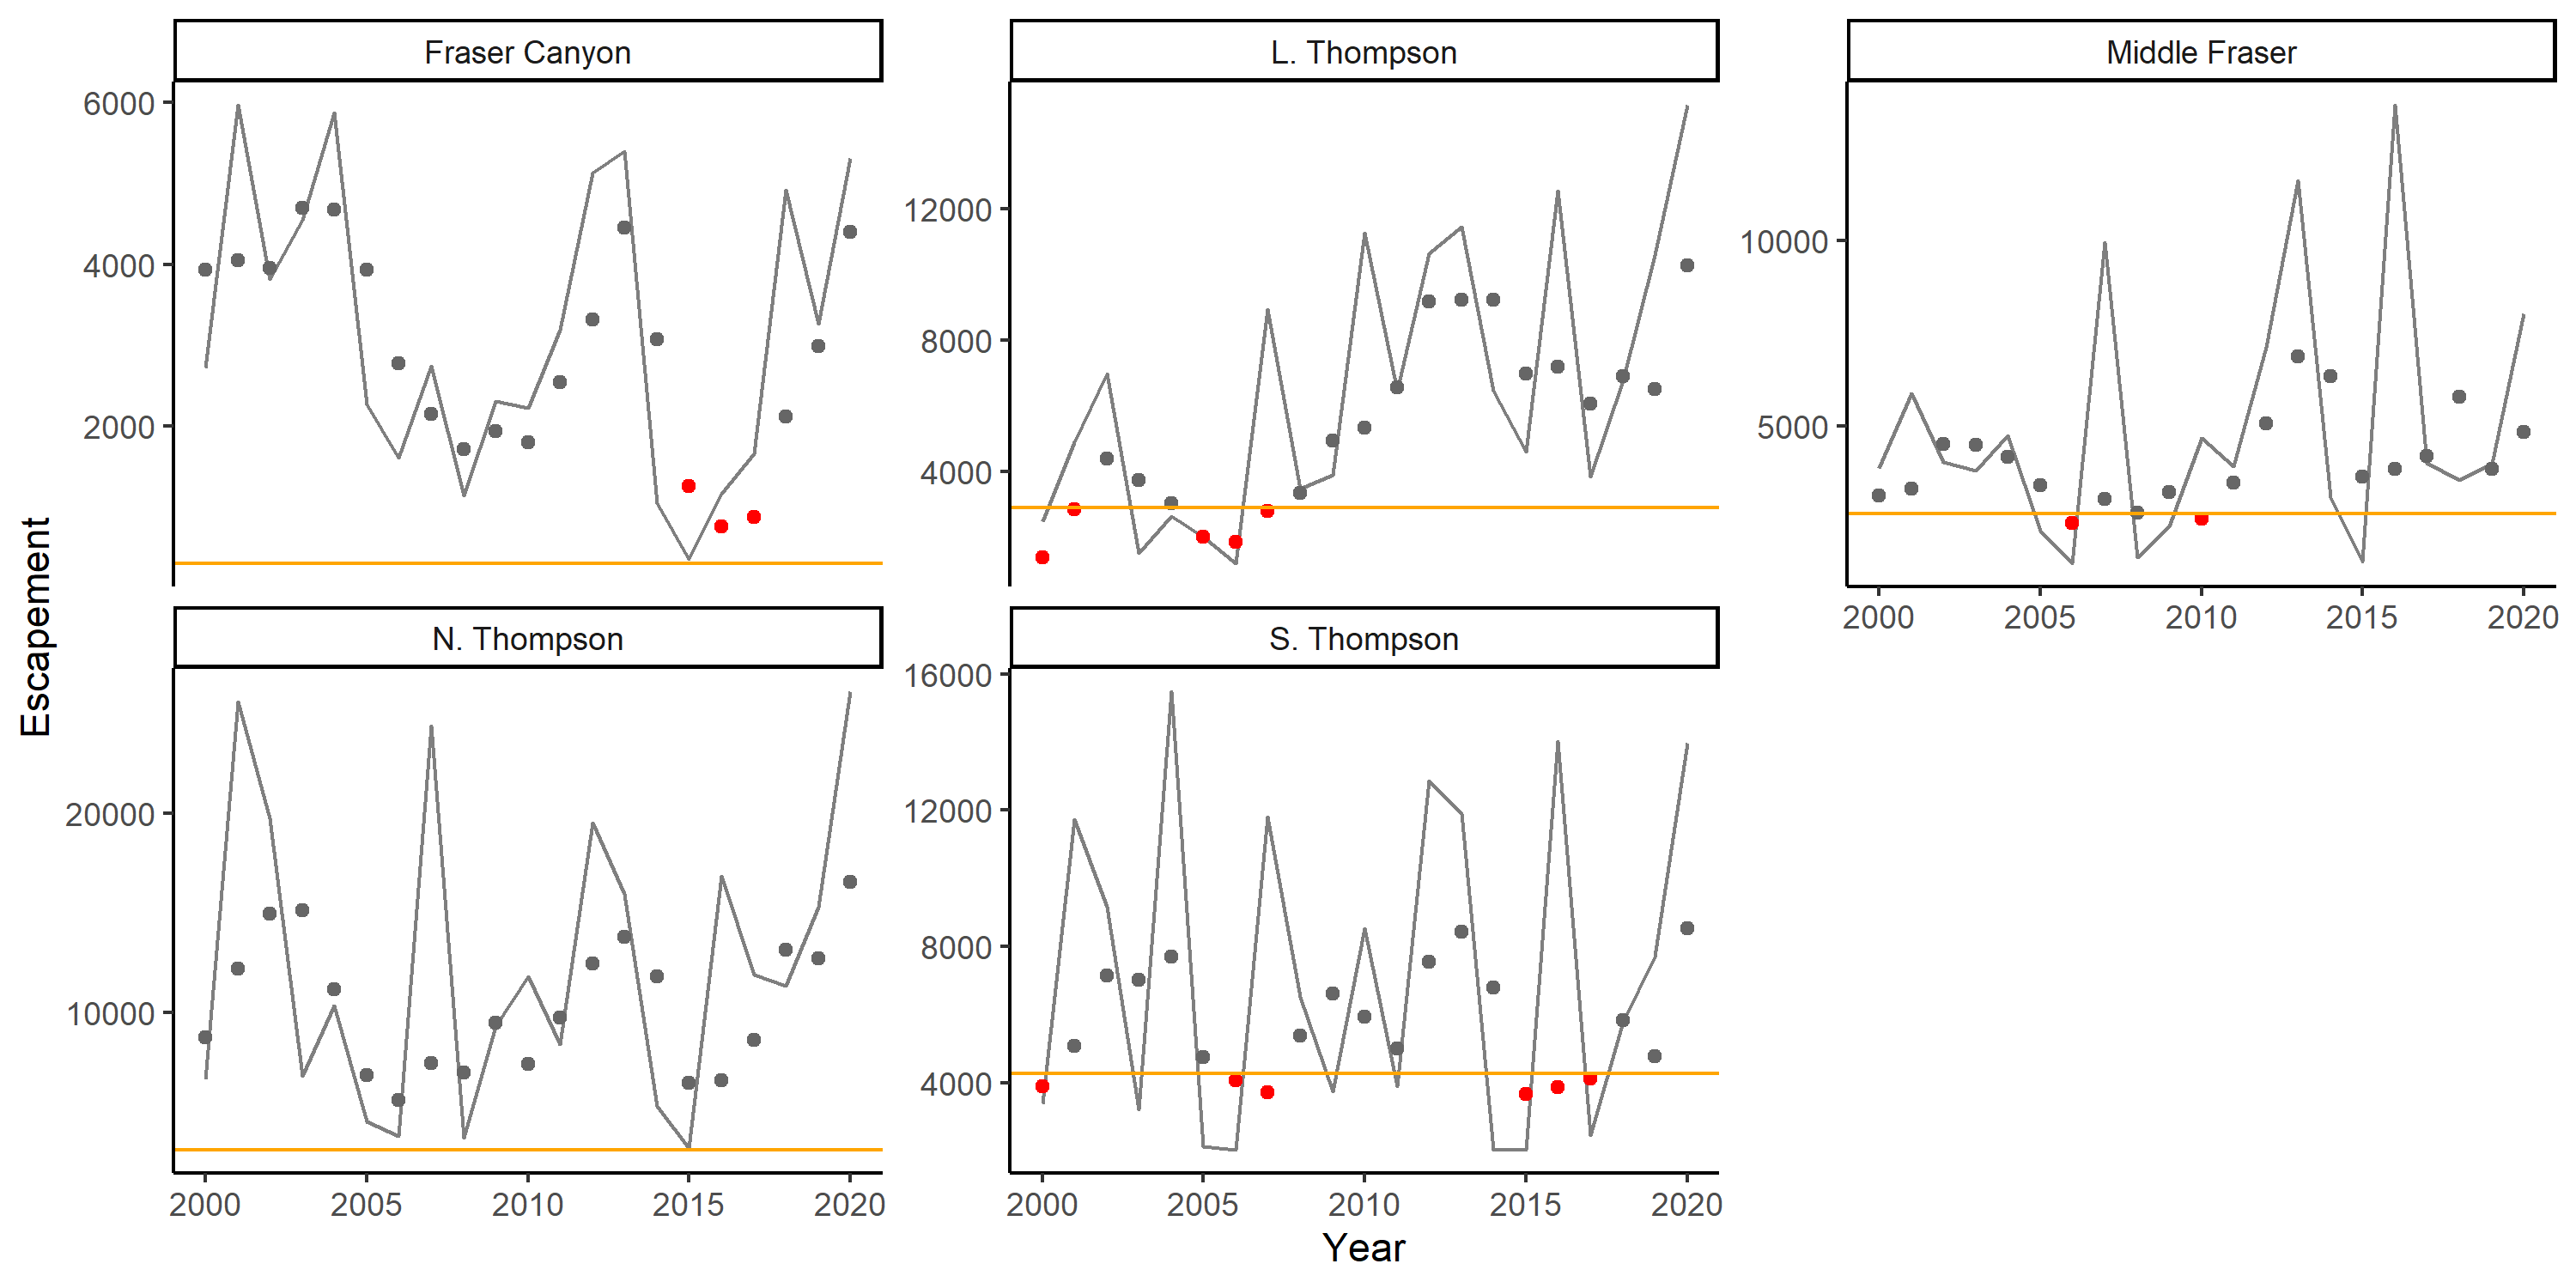
\includegraphics[width=6in]{figure/coho-CU-EscpSeries-wMultiStatus_Ricker_priorCap}}{Figure \ref{fig:coho-CU-multiDim-Ricker-Cap}} 

}

\caption{Escapement time series for five Interior Fraser Coho CUs shown as annual escapements (lines) and 3-year geometric mean escapements (dots). First geometric mean includes years 2008-2000. Grey dots indicate years in which all CUs had multidimensional rapid status assessments above red when Sgen was estimated using the Ricker\_priorCap model, while red dots indicate years in which one or more CUs had multidimensional status assessments in the red zone, which would trigger a breach of the LRP. Solid orange lines show estimates of Sgen from the Ricker\_priorCap model for comparison.}\label{fig:coho-CU-multiDim-Ricker-Cap}
\end{figure}
As a point of comparison, if a proportion-based LRP was based on all CUs being above the IFCRT distributional target, the LRP would have been breached in 4 of the 21 years between 2000 and 2020. Eight of the 11 sub-populations had generational average escapement drop below the 1000 spawner threshold in one or more years (Figure~\ref{fig:coho-Subpop-timeseries}). Sub-populations tended to differ in which years they dropped below the 1000 spawner threshold, which meant that the distributional target at least half of the subpopulations within each CU with greater than 1000 fish was more often met than not. All 11 subpopulations had generational average spawning abundances above 1000 spawners in 2020, indicating that the stock would be well above a proportion-based LRP based on the IFCRT-distributional target (Figure~\ref{fig:coho-Subpop-timeseries}).
\begin{figure}[htb]

{\centering \pdftooltip{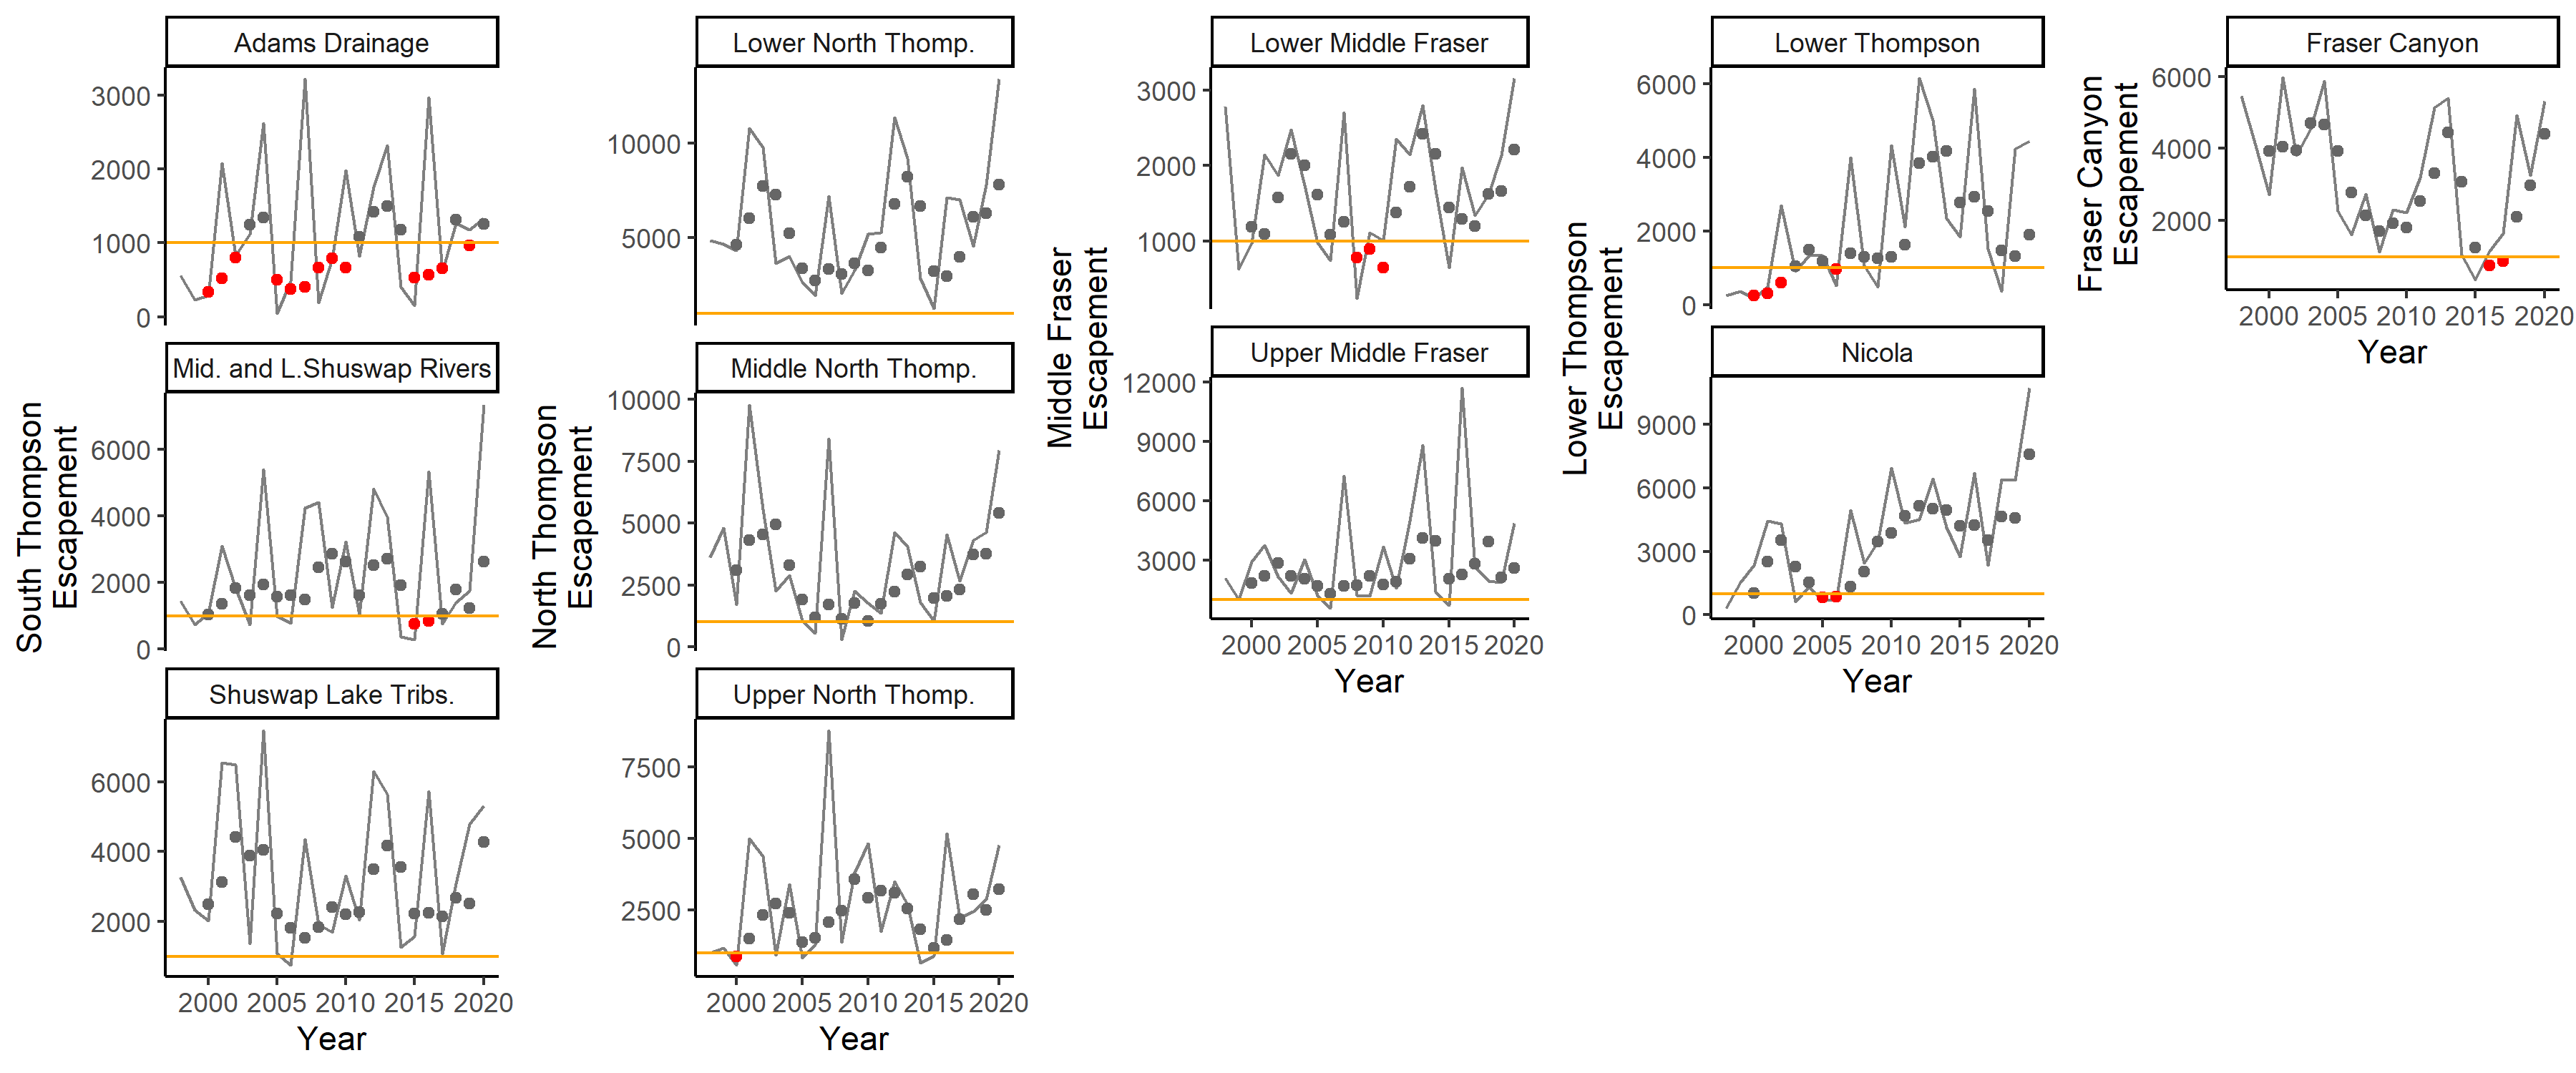
\includegraphics[width=6in]{figure/coho-Subpop-EscpSeries-wStatus}}{Figure \ref{fig:coho-Subpop-timeseries}} 

}

\caption{Escapement time series for 11 subpopulations of Interior Fraser Coho shown as annual escapements (lines) and 3-year geometric mean escapements (dots). Gray dots shows years in which the 3-year geometric mean escapement was above the 1000 fish threshold used to assess distributional status, while red dots show years in which the 1000 fish threshold was not met. CUs are represented by columns with labels long the y axis.}\label{fig:coho-Subpop-timeseries}
\end{figure}
\hypertarget{lrp-estimation-aggregate-abundance-logistic-regression-lrps}{%
\subsection{LRP ESTIMATION: AGGREGATE ABUNDANCE LOGISTIC REGRESSION LRPS}\label{lrp-estimation-aggregate-abundance-logistic-regression-lrps}}

\hypertarget{logistic}{%
\subsubsection{Methods}\label{logistic}}

We present aggregate abundance-based LRPs derived using logistic regressions with two of the Interior Fraser Coho benchmarks considered: \(S_{gen}\) and the IFCRT-distributional target. Because two different spawner recruit models were used to estimate \(S_{gen}\), we distinguish these models as `Logistic:Sgen-Ricker' and `Logistic:Sgen-priorCap' for the Ricker and Ricker\_priorCap models, respectively. We use the label `Logistic:IFCRT' to denote the case in which the IFCRT distributional target was used to develop the aggregate abundance logistic regression-based LRP. See Section~\ref{logisticMethods} for an overview of the approach used to calculate aggregate abundance-based LRPs using logistic regression.

When estimating logistic regression LRPs using \(S_{gen}\), we used an integrated modelling approach in which CU-level \(S_{gen}\) and the SMU-level LRP were simultaneously estimated. The integrated Sgen-LRP models had two components:
\begin{enumerate}
\def\labelenumi{(\roman{enumi})}
\item
  Stock-recruit models fit to each of the 5 CUs to estimate CU-level Sgen (Equation~\ref{eq:rickerSurv-IM} and Equations~\ref{eq:adjProd} -~\ref{eq:Sgen})
\item
  A logistic regression model fit to aggregated data to estimate the LRP as the aggregate abundance that has historically been associated with a specified probability of all CUs being above Sgen (Equations~\ref{eq:logistic} -~\ref{eq:logisticLRP})
\end{enumerate}
We initially considered a third version of the logistic regression model, in which we used the rapid multidimensional scanning tool to characterize CU status. Preliminary model evaluations led us to exclude this model due to poor fit. There were two factors limiting the establishment of a statistical relationship between multidimensional estimates of CU status and aggregate spawner abundance. First, the rapid multidimensional scanning tool relies on generational mean (smoothed abundances) to assess status of individual CUs against benchmarks, while our logistic regression approach uses raw (unsmoothed) aggregate abundance as a predictor variable. As a result, when logistic regressions were fit to CU status estimates from the multidimensional tool, there was a mismatch in the timing of abundance highs and lows. . This mismatch lead to a weak/non-existent relationship between SMU status and the raw (not smoothed) abundances. Using the generational mean of aggregate abundance as the predictor variable in the logistical regression fit instead of raw, annual abundance values introduced considerable autocorrelation in statuses. Future explorations of aggregate abundance logistic regression-based LRPs based on the rapid multidimensional scanning tool could account for the autocorrelation by including an AR(1) covariance structure. However, longer time-series and a wider spread of the data would be required to compensate for the additional parameter in the model.

The second limiting factor in establishing a statistical relationship between rapid multidimensional estimates of CU status and aggregate spawner abundance is that the rapid multidimensional scanning tool includes criteria that are not continuously tied to the CU abundance. For example, CU status can be determined based on trends, which is not congruent with logistic regression goal of identifying underlying relationship between aggregate abundance and CU statuses. In addition, the rapid multidimensional scanning tool includes absolute abundance thresholds (e.g.~generational mean should be above 1500 fish) that are not proportional to the size of a CU. These absolute benchmarks introduce a disconnect between the SMU abundance and status, even when there is high correlation between CUs, because small CUs will be more likely to be below the absolute threshold despite high aggregate abundances.

\textbf{\emph{Retrospective Analysis}}

We used retrospective analyses to examine the effect of time series length on logistic regression-based LRP estimates. Retrospective analyses were restricted to the most recent 6 years (2015-2020) because logistic model fits prior to 2015 were unable to converge on an LRP estimate. For each year between 2015 and 2020, we used data only available up to that year to calculate LRPs and associated confidence intervals.

To examine the effect of missing CUs on retrospective LRP estimates, we calculated LRPs using data from only a subset of the five Interior Fraser Coho CUs. We limited our analysis to missing data from either one or two CUs so that we had at least three CUs of available data when calculating the proportion of CUs above their benchmarks. For each missing data case, we calculated SMU aggregate status as
\begin{equation}
  AggStatus_t = \frac{\sum_{i}^{nCUs} S_{i,t}}{LRP'_t}
   \label{eq:status}
\end{equation}
where \(nCUs\) is the number of CUs being used (3 or 4) and \(LRP'_t\) is the LRP calculated in year \(t\) using only data from \(nCUs\). SMU-level status in a given year was calculated for all possible combinations of CUs available (5 combinations when nCUs = 4 and 10 combinations when nCUs = 3) to allow examination of the stability of status estimates among available combinations. Estimates of SMU status relative to LRPs were used to compare among missing CU scenarios instead of actual LRP estimates because the magnitude of the LRP will vary with the number and combination of CUs used. We evaluated the missing CU scenarios retrospectively for years 2017-2020.

\hypertarget{results-1}{%
\subsubsection{Results}\label{results-1}}

\textbf{\emph{LRP Estimates}}

Logistic regression model fits in 2020 from the integrated Logistic:Sgen-Ricker, Logistic:Sgen-priorCap and Logistic:IFCRT models are shown in Figure~\ref{fig:coho-IM-logisticFit2020}. All three logistic regression-based LRP methods were able to converge on a solution in 2020. Resulting LRPs for different \emph{p} thresholds are shown on the regression curves, as well as in Table~\ref{tab:logisticLRPs2020}. There was considerable uncertainty around predicted curves as seen in the large areas of gray shading in Figure~\ref{fig:coho-IM-logisticFit2020}.
\begin{figure}[htb]

{\centering \pdftooltip{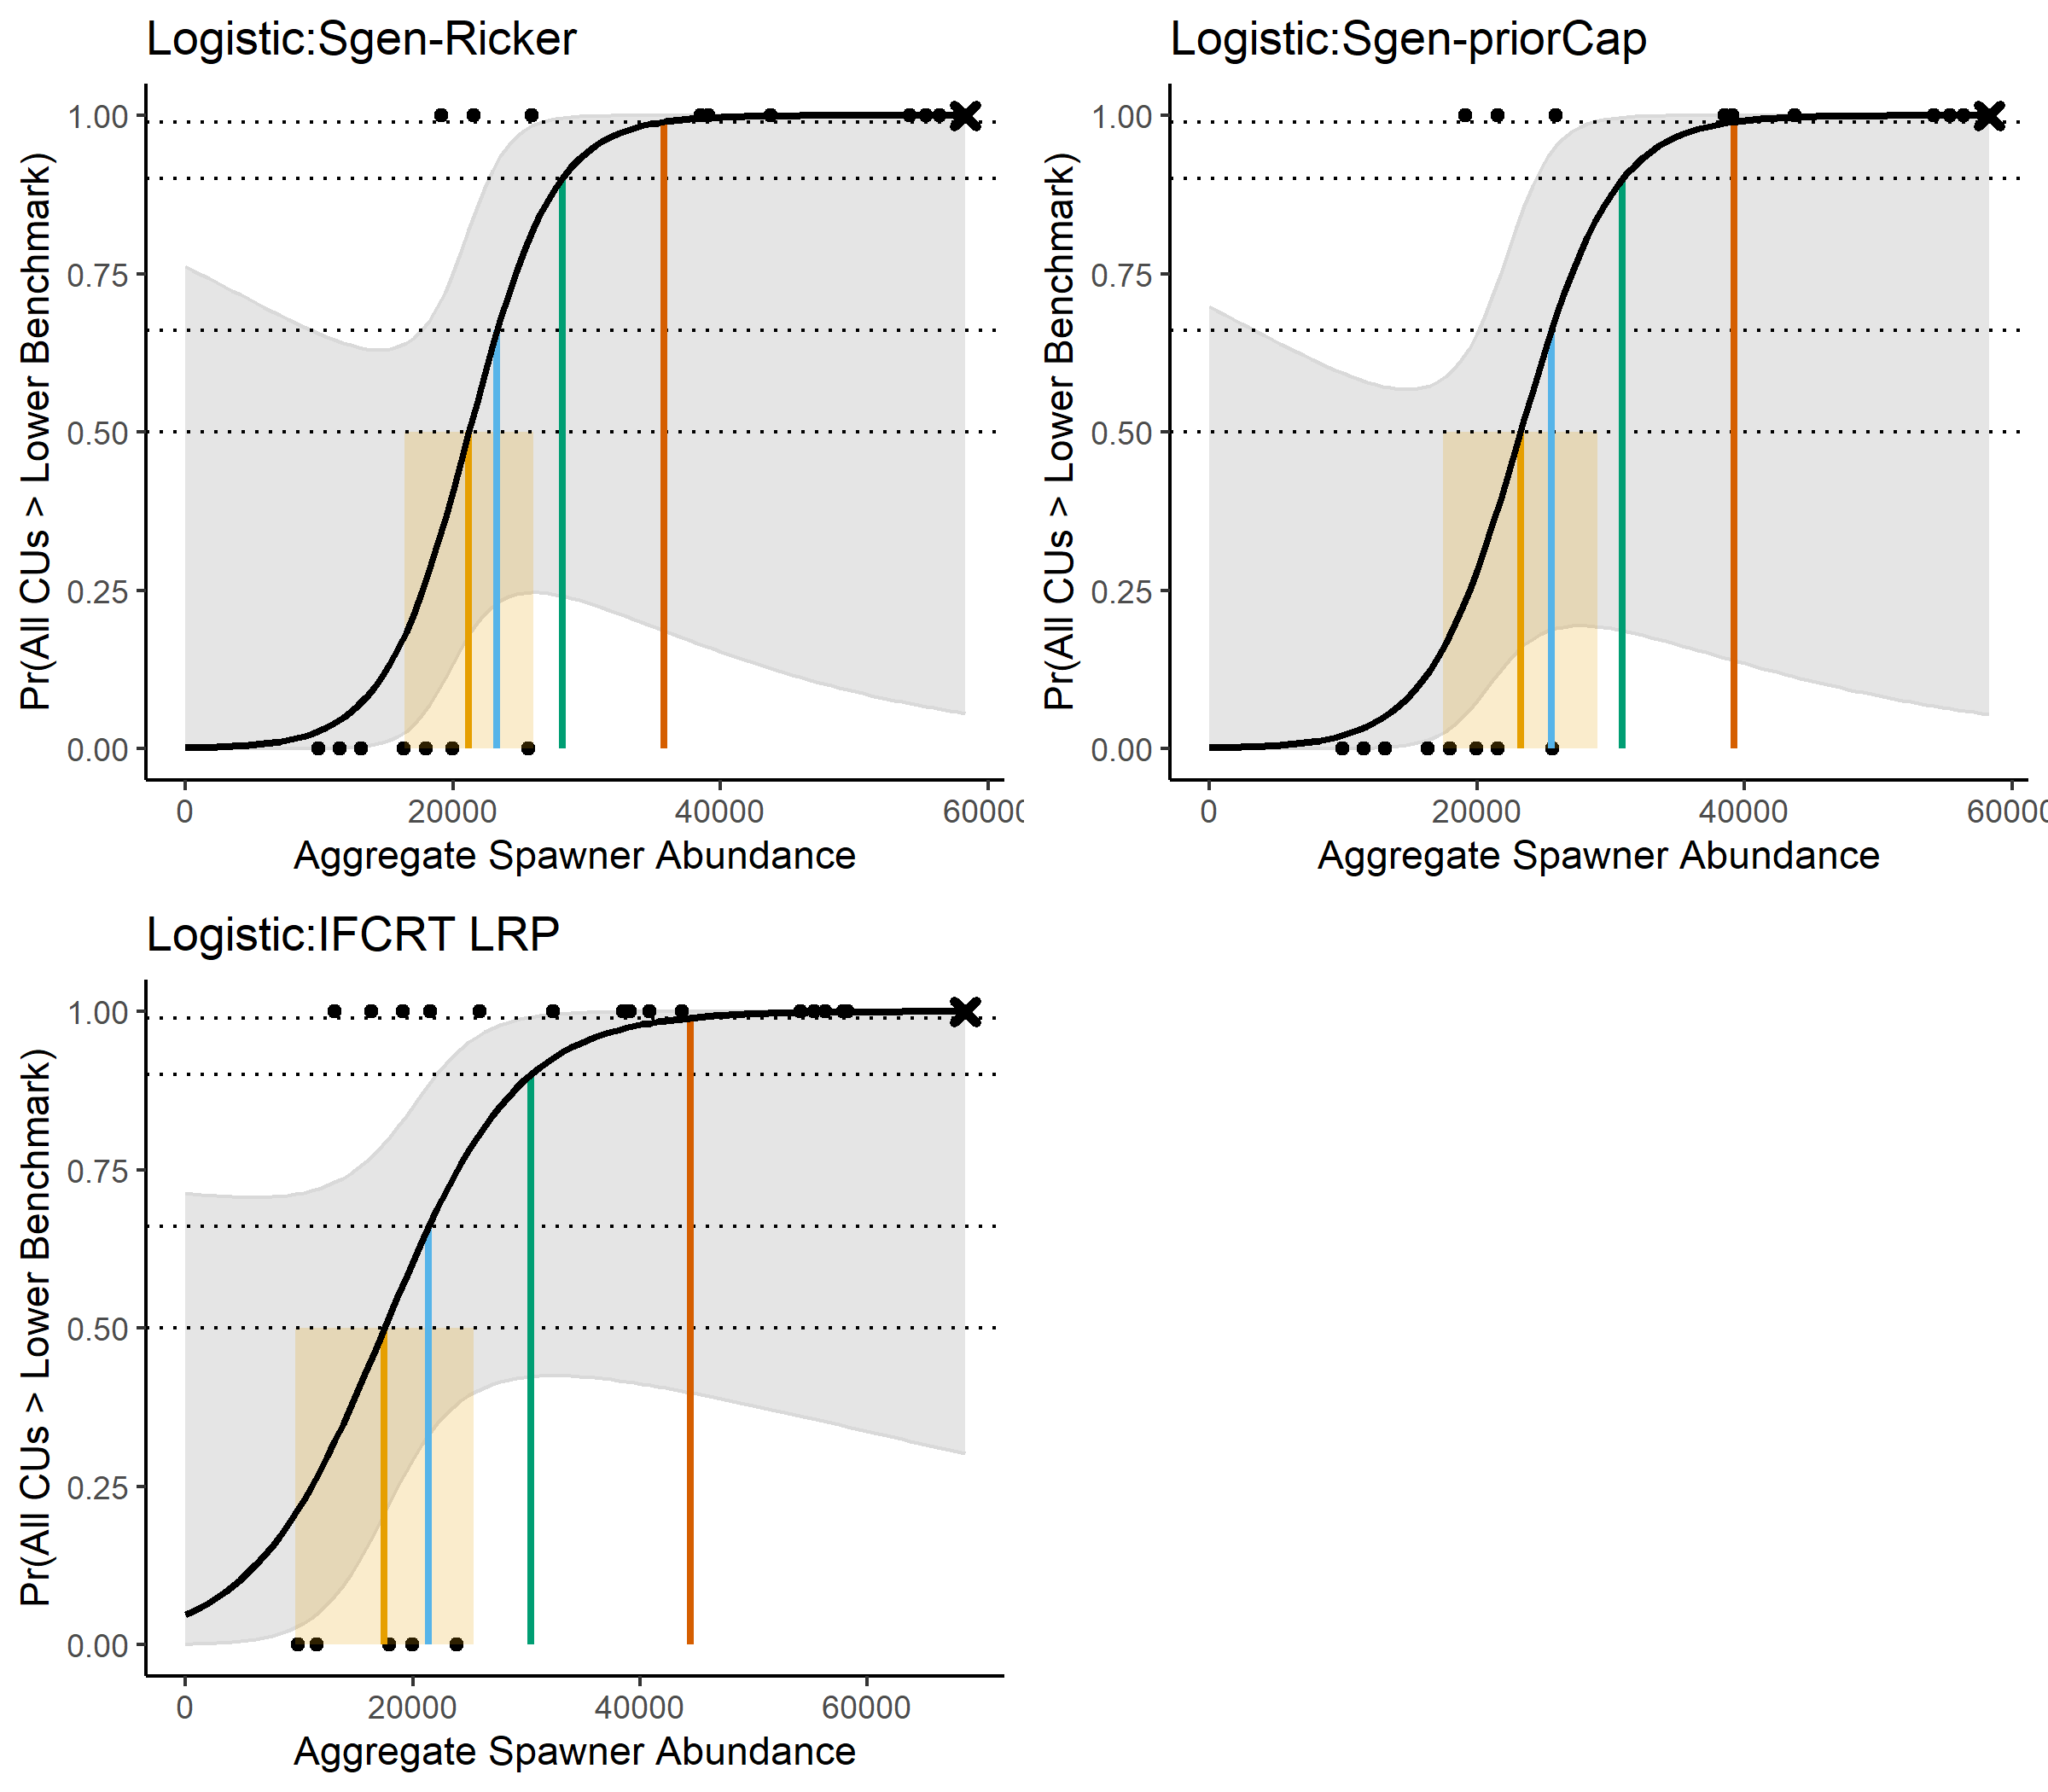
\includegraphics[width=0.5\linewidth]{figure/coho-all-LogisticLRP}}{Figure \ref{fig:coho-IM-logisticFit2020}} 

}

\caption{Logistic regression fit from the three logistic regression models: Logistic:Sgen-Ricker, Logistic:Sgen-priorCap and Logistic:IFCRT LRP model using data from 1998 - 2020. The yellow vertical line shows the LRP estimate based on the requirement of a 50\% probability of all CUs being above Sgen, while the yellow shaded region shows the associated 95\% confidence interval around the LRP. LRPs (MLE estimates only; no confidence intervals) for three alternative probability thresholds, 66\%, 90\%, and 99\%, are shown in blue, green, and orange, respectively.}\label{fig:coho-IM-logisticFit2020}
\end{figure}
When the Logistic:Sgen-Ricker model was used, aggregate abundance-based LRPs ranged from 21,189 to 35,737 spawners, depending on whether the required probability of all CUs being above Sgen was moderate (50\%) or very likely (99\%) (Table~\ref{tab:logisticLRPs2020}). LRPs increased across all probability levels when the carrying capacity was assumed higher under the Logistic:Sgen-priorCap model (Table~\ref{tab:logisticLRPs2020}). The higher \(S_{gen}\) values for most CUs under this alternative model formulation resulted in more historical years in which \textless{} 100\% of CUs were above \(S_{gen}\), resulting in a shift of the logistic curve to the right (Figure~\ref{fig:coho-IM-logisticFit2020}). LRPs based on the Logistic:Sgen\_priorCap model ranged from 23,245 to 39,200 spawners, depending on whether the required probability of all CUs being above Sgen was moderate (50\%) or very likely (99\%).

When CU status was based on the IFCRT distributional target, the fit of the logistic curve was more gradual than the two Sgen models due to a greater overlap in `successful' (all CUs \textgreater{} distributional target) and `unsuccessful' (\textless100\% of CUs above distributional target) years at low to moderate aggregate abundances. In 3 of the 6 years with aggregate abundances below 20,000 spawners, the distributional target was not met for all CUs (Figure~\ref{fig:coho-IM-logisticFit2020}). LRPs based on this model also became increasingly large at high probability thresholds (Table~\ref{tab:logisticLRPs2020}. The LRP based on a 99\% probability was 44,403 spawners, with a 95\% confidence interval extending from 15,102 - 73,703 spawners.\\
\begin{longtable}[]{@{}
  >{\raggedright\arraybackslash}p{(\columnwidth - 6\tabcolsep) * \real{0.29}}
  >{\raggedright\arraybackslash}p{(\columnwidth - 6\tabcolsep) * \real{0.24}}
  >{\raggedright\arraybackslash}p{(\columnwidth - 6\tabcolsep) * \real{0.24}}
  >{\raggedright\arraybackslash}p{(\columnwidth - 6\tabcolsep) * \real{0.24}}@{}}
\caption{\label{tab:logisticLRPs2020} Aggregate abundance based LRPs (with 95\% confidence intervals) from three different logistic regression-based LRP models. For each probability level, the LRP estimate represents that probability that all CUs will be above their lower benchmark.}\tabularnewline
\toprule
\begin{minipage}[b]{\linewidth}\raggedright
Probability
\end{minipage} & \begin{minipage}[b]{\linewidth}\raggedright
Sgen-Ricker
\end{minipage} & \begin{minipage}[b]{\linewidth}\raggedright
Sgen-priorCap
\end{minipage} & \begin{minipage}[b]{\linewidth}\raggedright
IFCRT
\end{minipage} \\
\midrule
\endfirsthead
\toprule
\begin{minipage}[b]{\linewidth}\raggedright
Probability
\end{minipage} & \begin{minipage}[b]{\linewidth}\raggedright
Sgen-Ricker
\end{minipage} & \begin{minipage}[b]{\linewidth}\raggedright
Sgen-priorCap
\end{minipage} & \begin{minipage}[b]{\linewidth}\raggedright
IFCRT
\end{minipage} \\
\midrule
\endhead
50\% (As likely as not) & 21,190 (16,383-25,996) & 23,245 (17,456-29,034) & 17,515 (9,695-25,336) \\
66\% (Likely) & 23,289 (17,364-29,215) & 25,547 (18,158-32,937) & 21,396 (13,418-29,375) \\
90\% (Very likely) & 28,145 (17,566-38,725) & 30,874 (18,129-43,620) & 30,372 (15,711-45,033) \\
99\% (Virtually certain) & 35,737 (16,525-54,949) & 39,200 (16,922-61,479) & 44,403 (15,102-73,703) \\
\bottomrule
\end{longtable}
\textbf{\emph{Logistic Regression Diagnostics}}

Logistic regression diagnostics showed that key regression assumptions were met, and that model fits were strong enough to support estimation of logistic regression-based LRPs from all three models (Table~\ref{tab:logisticDiagIFC2020}). The assumptions of linearity and lack of large outliers were met for all models. The assumption of linearity was demonstrated based on the Box-Tidwell test. This test evaluates the significance of adding a non-linear interaction term to the logit regression. We found that this additional interaction term was not significant, supporting the linearity assumption (Table~\ref{tab:logisticDiagIFC2020}). An examination of deviance residuals did not show any large outliers, i.e.~no residual values were greater than 2 for all three models. Observations were also found to be independent at all year lags examined for all three models.

The Wald Test showed that logistic model coefficient for aggregate abundance was marginally significant (p \textless{} 0.10). Pseudo-\(R^2\) statistics indicated a moderately strong relationship between aggregate abundance and the probability of all CUs being above their lower benchmarks, and the goodness of fit statistics indicated a significant fit of the model with aggregate abundance relative to the null model based on p-values less than 0.01. Finally, `out-of-sample' hit ratios representing classification accuracy as the proportion of successful predictions when one year of data was iteratively left out of the model fit, were relatively high at low probability thresholds, indicating good accuracy. This results was especially true for the Logistic:Sgen-Ricker and Logistic:Sgen-priorCap model which had hit ratios ranging between 0.83 and 0.87 at probability thresholds of 50\% and 66\%. Classification accuracy was lowest for all models at the 99\% probability threshold.

\renewcommand*{\arraystretch}{1.5}
\begin{table}[ht]
\centering
\caption{Model diagnostic statistics from Sgen:LRP, Sgen_priorCap:LRP, and Dist-LRP model fits. A description of diagnostic tests is provided in Section 2. Hit ratios are shown for all four probability thresholds considered.  The symbol '*' indicates a result that only marginally met the recommended criteria for demonstrating good model fit}
\begin{tabular}{p{2.5cm} p{2.5cm} p{2.5cm} p{2.5cm}}
\hline  
 Diagnostic Test  & Sgen-Ricker  & Sgen-priorCap & IFCRT \\
 Box-Tidwell p-value     & 0.44  & 0.94  & 0.79   \\
 Max. deviance residual  & 1.98  & 1.81  & 1.66   \\
 AR-1                    & -0.07 & 0.09  & 0.05   \\
 Wald p-values           & $0.07^*$& $0.06^*$& $0.09^*$ \\
 Goodness-of-fit p-value & <0.01 & <0.01 & <0.01  \\
 Pseudo-$R^2$            & 0.60  & 0.61  & 0.40   \\
 Hit Ratio (p= 50\%, 66\%, 90\%, 99\%) & 0.87, 0.83, 0.74, 0.70  & 0.83, 0.83, 0.83, 0.74 &  0.76, 0.71, 0.76, 0.52 \\
\hline
\end{tabular}
\label{tab:holt-tab6}
\end{table}
Sample sizes were small due to the short time series available for Interior Fraser Coho; only 23 years of observations were available to fit logistic regression models. \protect\hyperlink{ref-peduzziSimulationStudyNumber1996}{Peduzzi et al.} (\protect\hyperlink{ref-peduzziSimulationStudyNumber1996}{1996}) recommend a minimum requirement of 10 data points for the least frequent outcome based on their simulation studies in the field of clinical epidemiology. In our case, the least frequent outcome was the failure of all CUs to be above their benchmarks (i.e., 0). We were not able to make this minimum requirement for any of our model fits; we had only 7, 8, and 5 data points at the least frequent outcome for the Logistic:Sgen-Ricker, Logistic:Sgen-priorCap, and Logistic-IFCRT models, respectively. Based on the current ratio of successes and fails in the data, the estimated minimum sample sizes that would be required to meet the criteria of \protect\hyperlink{ref-peduzziSimulationStudyNumber1996}{Peduzzi et al.} (\protect\hyperlink{ref-peduzziSimulationStudyNumber1996}{1996}) ranged from 26 to 42 years. However, despite small sample sizes, hit ratios are high for all models at p = 50\%. As a result, we suggest that logistic regression-based LRPs may still be useful for this SMU. We proceeded with retrospective analyses in order to examine how sensitive LRPs based on these model fits were to variations in the level of available data.

\textbf{\emph{Retrospective Analysis}}

We started the retrospective analyses for the three Logistic regression models in 2010. Throughout the time series, the Logistic:Sgen-Ricker did not convert when the estimates were truncated to 2013 and 2014. The Logistic:Sgen-priorCap model was unable to converge on an LRP estimate in 2018. All three models showed some fluctuations in LRP estimates over time (Figure~\ref{fig:coho-retroLRPs}). The Logistic:IFCRT model tended to produce the lowest estimates of LRPs over time, followed by the Logistic:Sgen-Ricker and the Logistic:Sgen-priorCap.
\begin{figure}[htb]

{\centering \pdftooltip{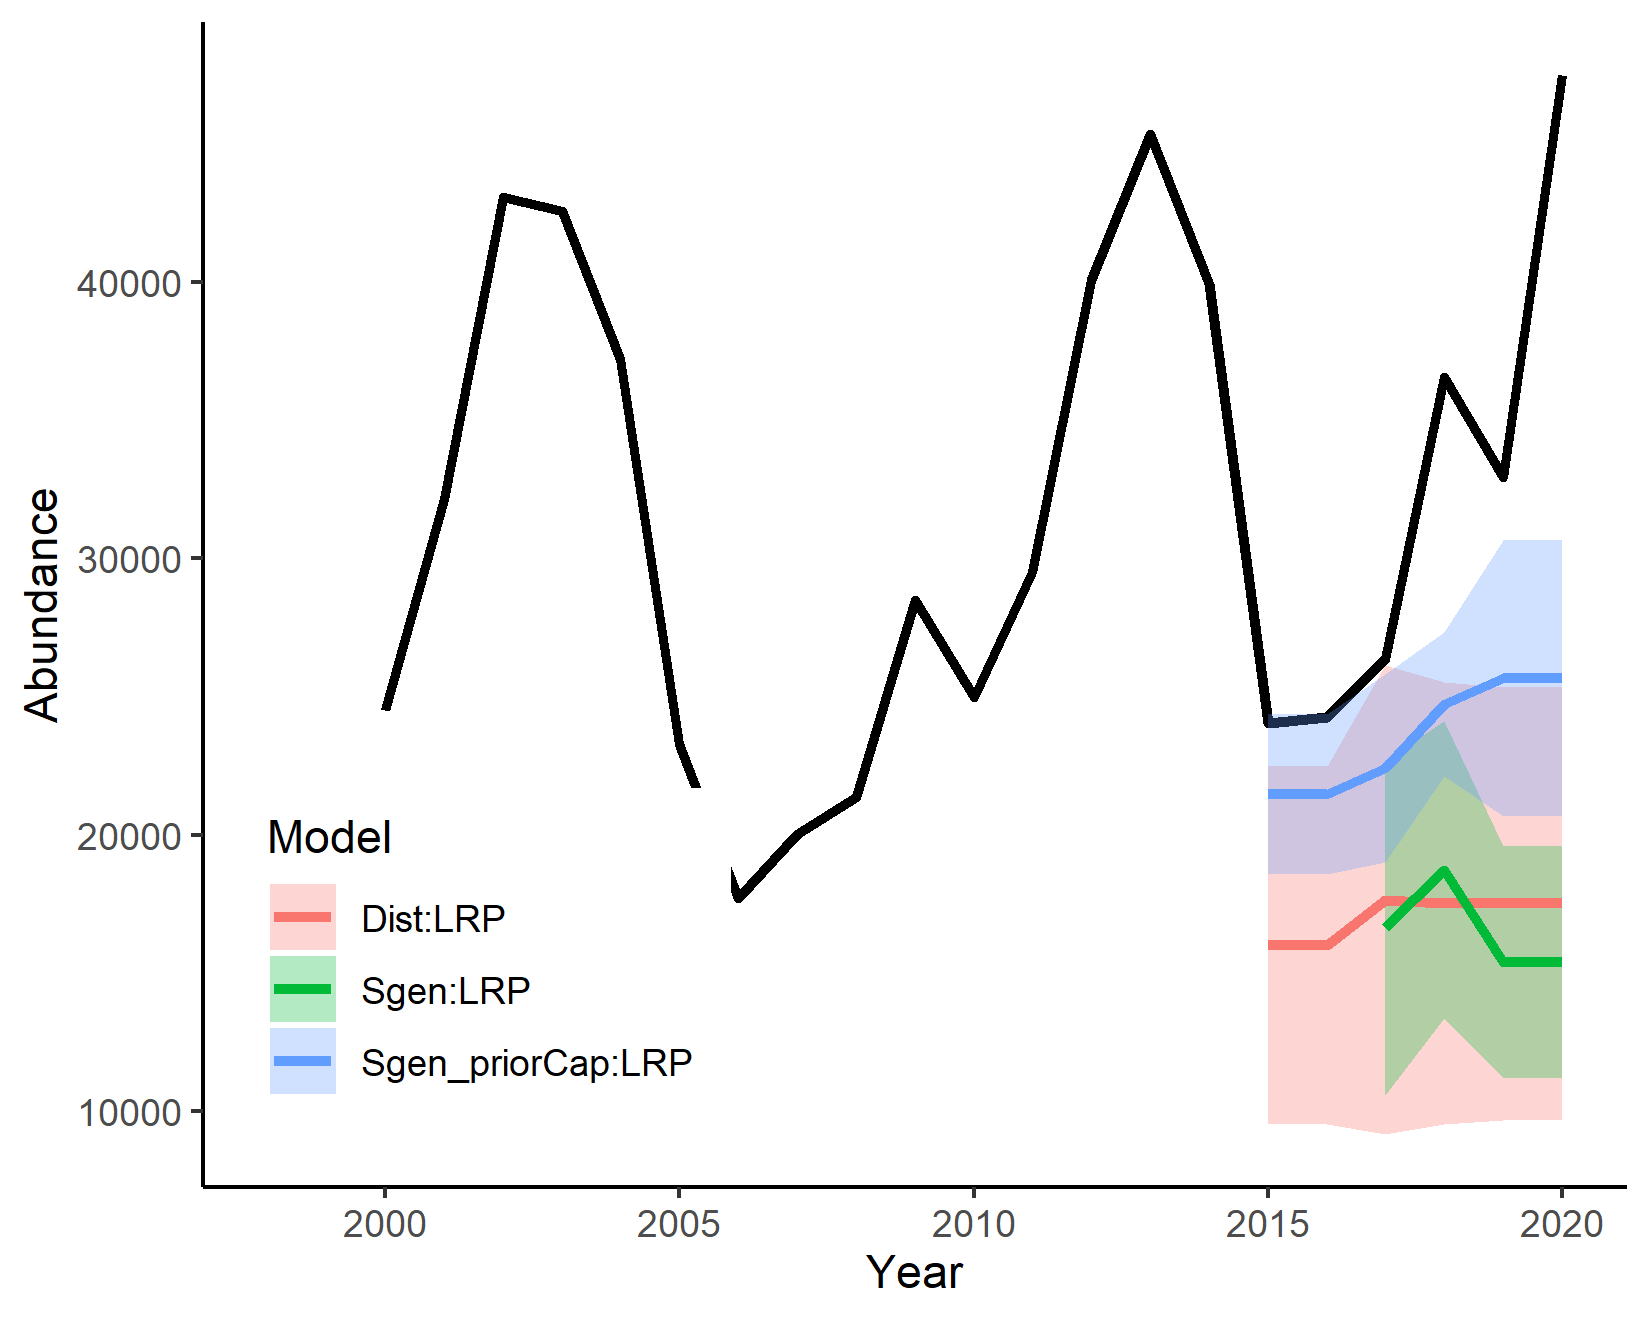
\includegraphics[width=0.5\linewidth]{figure/coho_LRP_compareRetro}}{Figure \ref{fig:coho-retroLRPs}} 

}

\caption{Three-year geometric mean of aggregate spawning abundance for the Interior Fraser Coho SMU (black line) and associated time series of retrospective LRPs from logistic regression-based estimation methods. LRPs are based on a 50\% probability that all CUs will be above their lower benchmarks. Annual LRP estimates are shown as maximum likelihood values (coloured lines) and associated 95\% confidence intervals (shaded areas).}\label{fig:coho-retroLRPs}
\end{figure}
\linebreak

When the Logistic:Sgen-Ricker model was applied retrospectively to missing data scenarios with four out of the five CUs, only a subset of scenarios had LRP estimates that converged on a solution (Figure~\ref{fig:coho-IM-missingCUs}). All the five possible combinations of four CUs had estimates in 2017-2019, while only four had estimates in 2020. For scenarios in which LRP estimates were possible, estimates of aggregate status (Equation~\ref{eq:status}) were often close to the estimate obtained when all 5 CUs were used, and always overlapped with the 95\% confidence interval of the full data estimate. The Logistic:Sgen-Ricker model was less likely to converge on a solution when data from only three CUs were used. This pattern was especially true for 2020 when only 6 out of the 10 possible combinations had estimates. For scenarios that were able to converge, aggregate status estimates from 3 CUs tended to be more uncertain than 4- and 5-CU estimates, and showed larger deviations from estimated status when all CUs were used. One missing data scenario in 2019 had a status estimate that fell outside of the 95\% confidence interval of the full data estimate.
\begin{figure}[htb]

{\centering \pdftooltip{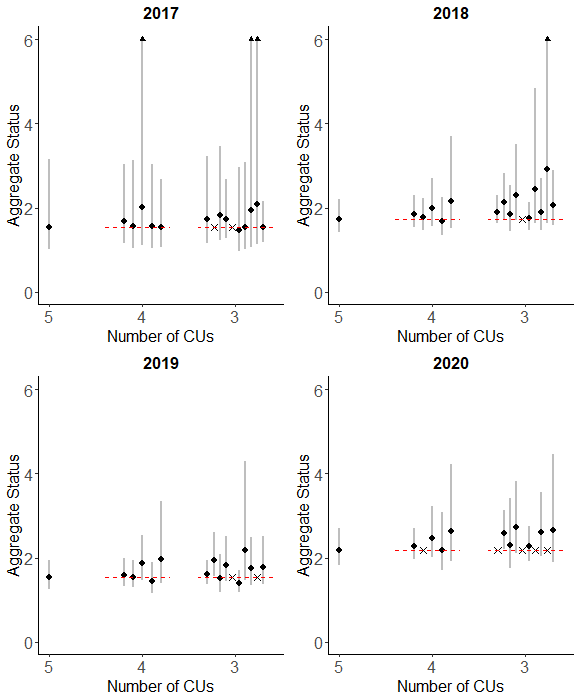
\includegraphics[width=0.8\linewidth,height=0.5\textheight]{figure/coho-StatusByNCUs-IndivRickerSurv-50}}{Figure \ref{fig:coho-IM-missingCUs}} 

}

\caption{Retrospective estimates of aggregate status (with 95\% confidence intervals) from the Logistic:Sgen-Ricker  model under different scenarios about missing CUs, where aggregate status is characterized as the recent generational mean of aggregate abundance / LRP. LRPs are based on a 50\% probability that all CUs will be above their lower benchmarks. The set of status estimates associated with each number of CUs on the x-axis represents all possible combinations of CUs created by selecting that number from the 5 available CUs.  Red dashed lines show the maximum likelihood estimate when no data is missing (i.e., all 5 CUs) for comparison with the missing data scenarios.}\label{fig:coho-IM-missingCUs}
\end{figure}
\linebreak

When the Logistic:Sgen-priorCap model was applied to missing data scenarios in which four out of five CUs had data, LRP estimates were only available for two of the five CU combinations (Figure~\ref{fig:coho-IMCap-missingCUs}). For scenarios in which LRP estimates were available, status was poorly estimated with the estimate often falling outside of the 95\% confidence interval of the full data estimate. While convergence was more frequent when only three CUs were used, estimates had high uncertainty and were variable among scenarios. Several of the status estimates from three-CU scenarios fell outside of the 95\% confidence interval for the full data case. In the year 2018 the model did not converge when all CUs were included, but estimates for missing CU scenarios were available.

The failure of both the Logistic:Sgen-Ricker and Logistic:Sgen-priorCap models to converge in some years is a function of low sample sizes in the available data set, such that the removal of one or two CUs results in a failure of the logistic regression model to converge on a solution. For example, for the Logistic:Sgen-Ricker model, the South Thompson CU is an influential CU. Removing it from the characterization of `successful' and `failure' years, as well as the aggregate abundance used to fit the logistic regression, means that the model cannot converge on a solution because there was no overlap in aggregate abundance levels associated with `successes' and `failures,' which is a requirement for logistic regression model fits. For the Logistic:Sgen-priorCap model, several CUs are influential due to higher \(S_{gen}\) estimates compared to the Logistic:Sgen-Ricker model. Because several different CUs contribute to `failure' years, in which CU-level abundances drop below \(S_{gen}\), there is higher sensitivity to the removal of any one of these CUs.
\begin{figure}[htb]

{\centering \pdftooltip{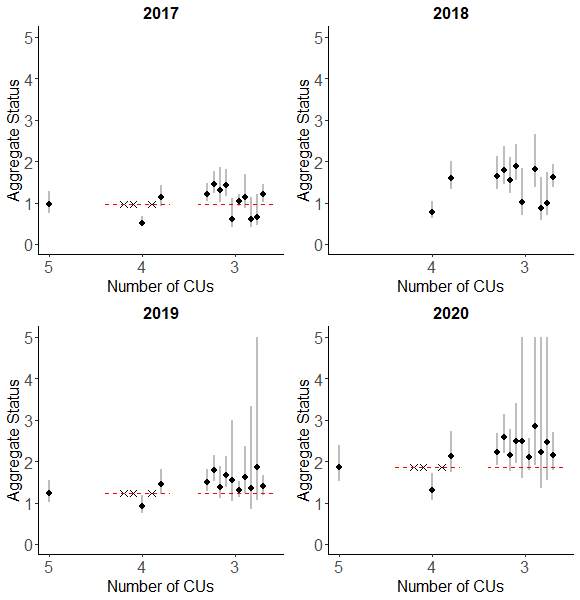
\includegraphics[width=0.8\linewidth]{figure/coho-StatusByNCUs-IndivRickerSurvCap-50}}{Figure \ref{fig:coho-IMCap-missingCUs}} 

}

\caption{Retrospective estimates of aggregate status (with 95\% confidence intervals) from the Sgen\_priorCap:LRP model under different scenarios about missing CUs, where status is characterized as the recent generational mean of aggregate abundance / LRP. LRPs are based on a 50\% probability that all CUs will be above their lower benchmarks. See Figure xx caption for more details.}\label{fig:coho-IMCap-missingCUs}
\end{figure}
\linebreak

LRPs based on the Logistic:IFCRT model could be estimated for all four-CU data scenarios in all years (Figure~\ref{fig:coho-distributional-missingCUs}). Resulting estimates of SMU status were similar to the full data estimate for four of the five CU combinations. Status estimates were highest and most uncertain when the South Thompson CU was dropped from the analysis (i.e., the last of the five four-CU combinations shown for each year in Figure~\ref{fig:coho-distributional-missingCUs}). This pattern is due the 2015 data point for South Thompson CU, which is a red status and an influential observation that has a large impact on the shape of the fit model. When that CU is removed, the status goes up. . For missing data scenarios in which only three CUs were included, status estimates often had higher uncertainty than the four-CU or full data scenarios, and showed high variability among scenarios in estimated status.
\begin{figure}[htb]

{\centering \pdftooltip{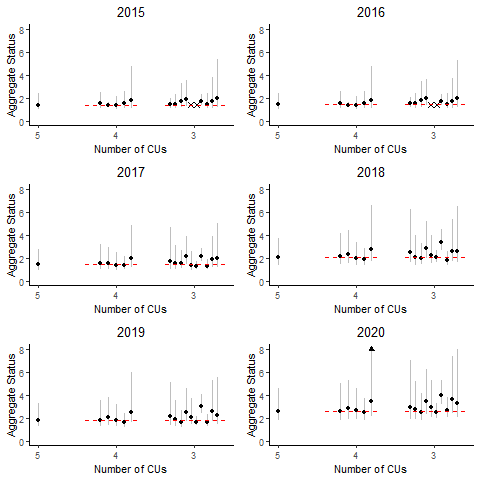
\includegraphics[width=0.8\linewidth]{figure/coho-StatusByNCUs-SPopAbundThreshST-50}}{Figure \ref{fig:coho-distributional-missingCUs}} 

}

\caption{Retrospective estimates of aggregate status (with 95\% confidence intervals) from the Dist:LRP model under different scenarios about missing CUs, where status is characterized as the recent generational mean of aggregate abundance / LRP. LRPs are based on a 50\% probability that all CUs will be above their lower benchmarks. See Figure xx caption for more details.}\label{fig:coho-distributional-missingCUs}
\end{figure}
\linebreak

\hypertarget{lrp-estimation-aggregate-abundance-projection-based-lrps}{%
\subsection{LRP ESTIMATION: AGGREGATE ABUNDANCE PROJECTION-BASED LRPS}\label{lrp-estimation-aggregate-abundance-projection-based-lrps}}

\hypertarget{methods-1}{%
\subsubsection{Methods}\label{methods-1}}

Forward projections of each of the five CUs with the Interior Fraser Coho SMU were done using the \texttt{samSim} modelling tool (Appendix~\ref{app:samsim-appendix}). Parameters characterizing population dynamics, marine survival rates, and exploitation rate were derived directly from data sets described in Section~\ref{cohoData}. Base case parameters and alternative parameter values tested in sensitivity analyses are provided in Table~\ref{tab:coho-BaseProjectPars}. Additional details on key model parameterizations and sensitivity analyses are also described in text below.

Projection model outputs were used to estimate projection-based LRPs using the methods described on Section~\ref{projectedMethods}. Forward projections were run for 30 years over 20,000 simulation trials. The high number of simulation trials was required to stabilize LRP estimates given the binning of aggregate escapement in 200-fish intervals to identify LRPs based on probability thresholds. We found that running projections over longer periods, such as 100 years, gave similar results as our 30 year time horizon.

\textbf{\emph{Stock recruitment dynamics}}

Stock recruitment parameters for all five CUs were drawn from joint posterior distributions obtained by fitting the two stock recruit models described in Section~\ref{cohoSgen} (Ricker and Ricker\_priorCap) to available spawner-recruit data using Bayesian Markov Chain Monte Carlo (MCMC) estimation. Bayesian estimation was done using tmbStan (Kristensen 2019), which is an R package that allows MCMC samples to be drawn from a TMB model object using rStan (Guo et al.~2020). Three MCMC chains were run for 14,000 iterations, with the first half of each chain excluded from the final posterior sample. Resulting joint posterior distributions included 21,000 samples. Posterior sampling was initiated at the MLE estimates for each model formulation. Neither model showed signs of convergence failure based on our examination of Rhat and effective sample size diagnostics, as well as visual inspections of marginal posterior distributions. A summary of marginal posterior distributions for each stock recruitment parameter (\(\alpha\), \(\beta\), \(\gamma\), and \(\sigma\)) is provided in Appendix~\ref{app:coho-appendix}.

The two stock recruitment models, Ricker and Ricker\_priorCap, were treated as two alternative hypotheses about stock recruitment dynamics, which we compare against each other. We also considered a simple model-averaging approach, in which we equally weighted the two stock recruit models by combining projections prior to calculating a projection-based LRP. Additional sensitivity analyses described below were only done using the base Ricker model.

\textbf{\emph{Covariance in recruitment residuals}}

We parameterized correlations in recruitment residuals among CUs from MLE predictions of pairwise correlations from spawner recruit model fits. The correlation matrix from the base Ricker model fit is shown in Figure~\ref{fig:coho-recruitResid-Ricker}. Correlation values for the Ricker\_priorCap model were similar (not shown).

We initially attempted to reduce covariation in spawner abundances among CUs by scaling correlations in recruitment residuals (i.e., scalar \textless{} 1). However, we found that scalars had little effect on projected correlations in spawner abundances among CUs due to the shared marine rate coefficient dominating among-CU variability in recruitment. We therefore used sensitivity analyses of the level of variability in marine survival coefficients among CUs to drive patterns of covariation in spawner abundance, as described below. This approach differs from that taken for WCVI Chinook (Section~\ref{WCVIchinookChapter}.
\begin{figure}[htb]

{\centering \pdftooltip{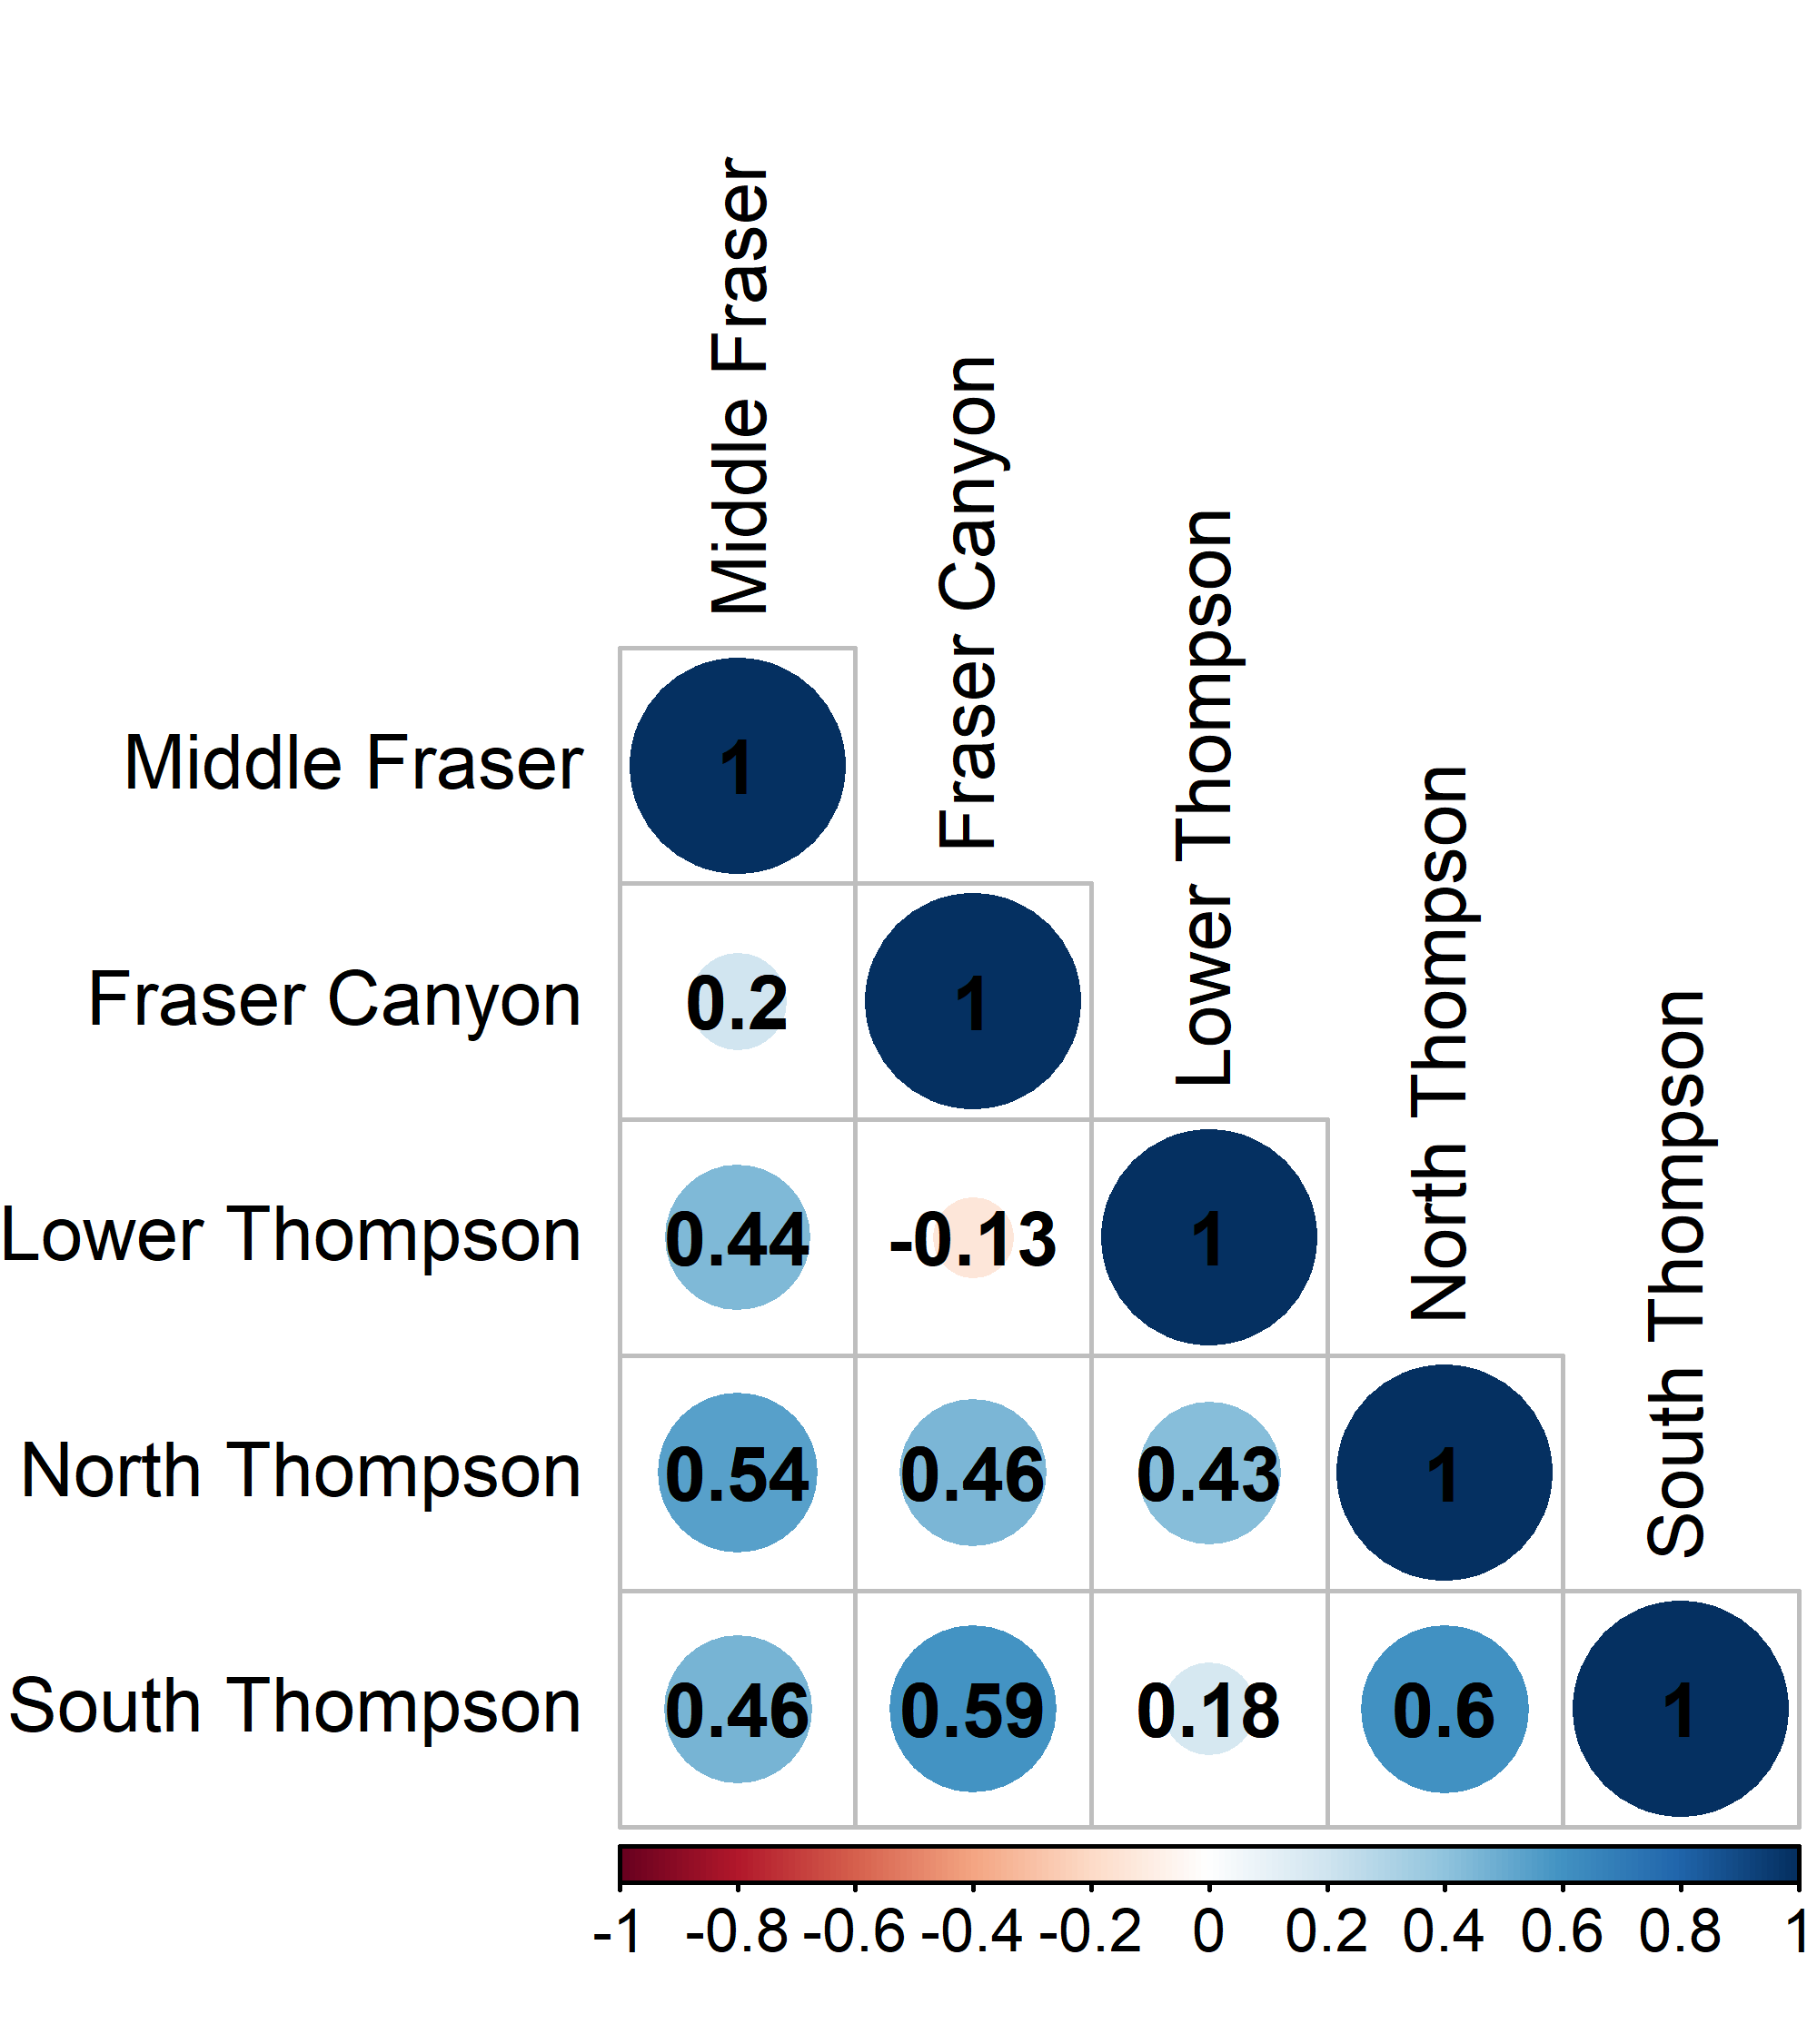
\includegraphics[width=0.5\linewidth]{figure/coho-RecuitResidCorrelation-Ricker}}{Figure \ref{fig:coho-recruitResid-Ricker}} 

}

\caption{Bubble plot of correlations in recruitment residuals among CUs from base Ricker model fit.}\label{fig:coho-recruitResid-Ricker}
\end{figure}
\linebreak

\textbf{\emph{Variability in marine survival coefficient among CUs}}

When fitting spawner recruit models to data, we followed the approach of \protect\hyperlink{ref-kormanEvaluationFrameworkAssessing2019}{Korman et al.} (\protect\hyperlink{ref-kormanEvaluationFrameworkAssessing2019}{2019}) and \protect\hyperlink{ref-arbeiderInteriorFraserCoho2020}{Arbeider et al.} (\protect\hyperlink{ref-arbeiderInteriorFraserCoho2020}{2020}) in assuming that all CUs experienced the same marine survival rate for given sea-entry year, and that the marine survival coefficient, \(\gamma\), was constant both among CUs and among years. When projecting CUs forward, we maintained this assumption in our base case by generating a single marine survival rate for each sea entry year and setting \(\sigma_{\gamma}\) = 0, where \(\sigma_{\gamma}\) is the standard deviation of among-CU variability in \(\gamma\) such that \(\gamma_i \sim Normal(\bar{\gamma}, \sigma_{\gamma})\). We used sensitivity analyses on \(\sigma_{\gamma}\) to test the effect of changes in spawner abundance covariation among CUs on projected LRP estimates. Three alternative levels of \(\sigma_{\gamma}\) were used in sensitivity analyses: \(\sigma_{\gamma}\) = 0.045, 0.0675, and 0.09. We selected these levels to cover a range between 0 and 0.09, where 0.09 was the standard deviation of the estimated marginal posterior distribution for \(\gamma\) from our Ricker stock recruitment model fit.

The resulting correlations in spawner abundances from the projections are shown in Figure~\ref{fig:coho-sigGammaCorrelation}. In the forward projections, pairwise correlations in projected spawner abundances among CUs for the base case assumption of \(\sigma_{\gamma}\) = 0 were similar to observed pairwise correlations in spawner abundances among CUs. Increasing \(\sigma_{\gamma}\) resulted in decreased among-CU correlation in projected spawner abundances.
\begin{figure}[htb]

{\centering \pdftooltip{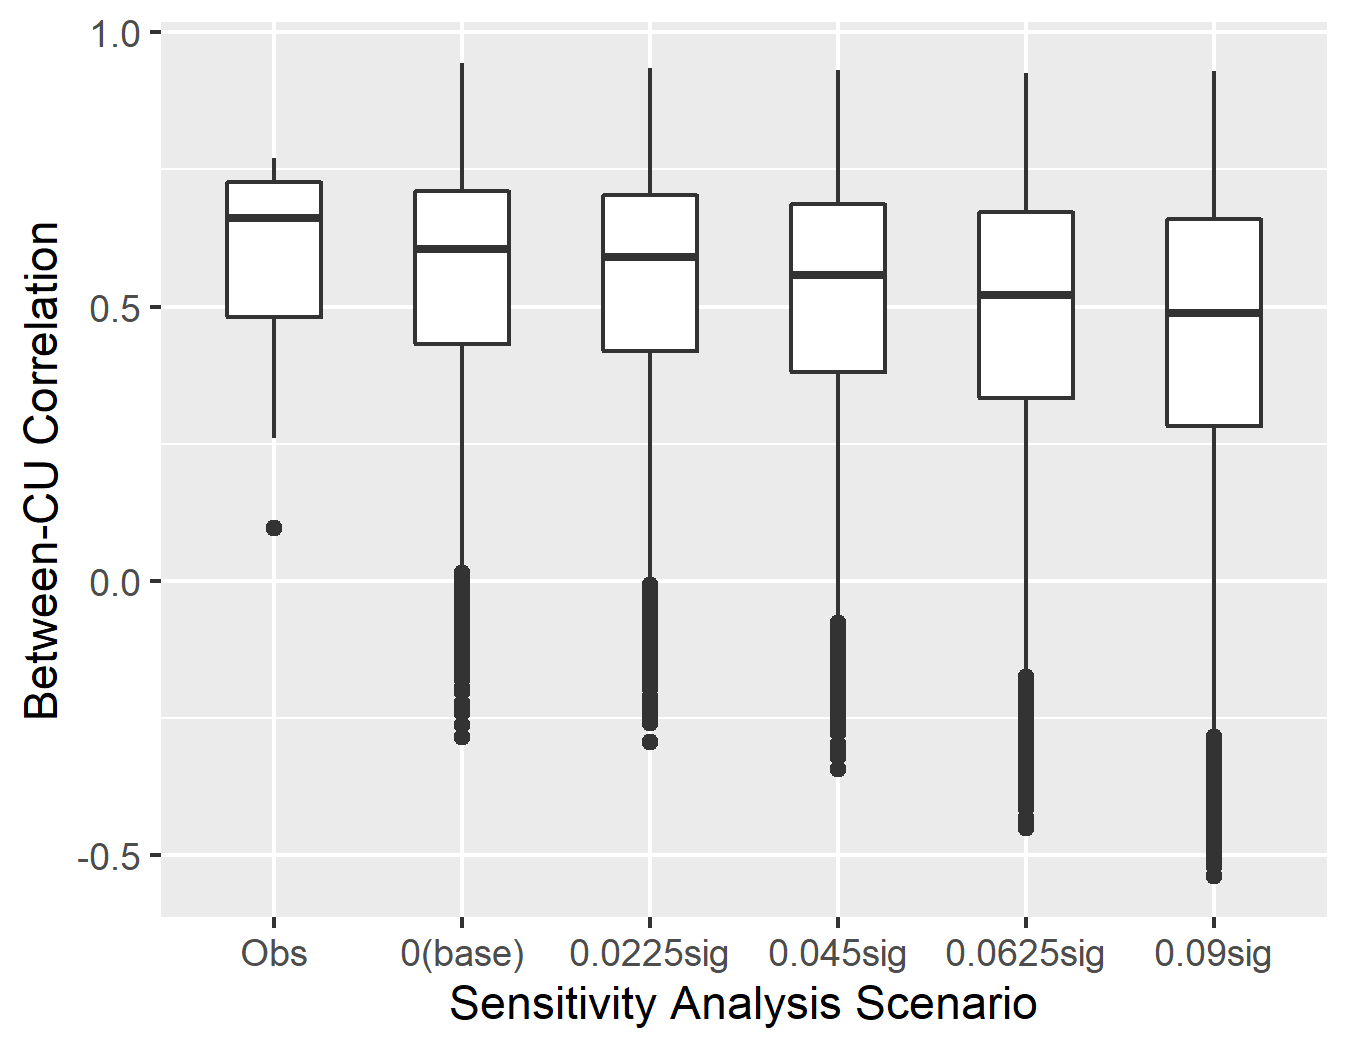
\includegraphics[width=0.5\linewidth]{figure/coho-corrEffect-sigGamma}}{Figure \ref{fig:coho-sigGammaCorrelation}} 

}

\caption{Distribution of correlations of spawner abundances among CUs for observed data between 1998 and 2021 and projected time-series under alternative assumptions about the standard deviation on the marine survival co-efficient among CUs for the base Ricker model formulation.}\label{fig:coho-sigGammaCorrelation}
\end{figure}
\linebreak

\textbf{\emph{Variability in age proportions of recruits among CUs}}

Annual variability in the age structure of returns was generated from a multivariate logistic distribution parameterized using CU-specific time series of proportions at age. The underlying average age structure for each CU was set at the average from the available time series (brood years 1998 - 2016), while annual deviations from underlying age-specific means were drawn from a multivariate logistic distribution. Annual deviations were held constant among all CUs; however, the scale of annual deviations was controlled by the variability parameter \(\tau\), which was estimated individually for each CU. This meant that while all CUs simultaneously experienced increases or decreases in a given year, the magnitude of the increase or decrease was CU-specific. Annual deviations were held constant among CUs to represent the strong co-variation in proportions at age seen in available time series for Interior Fraser Coho, especially since 2010 (Figure~\ref{fig:coho-recruitResid-Ricker}). When the constraint of constant annual deviations was removed, generated proportion at age data was much more variable than observed data, which was considered to be unrealistic.

Annual variability in the age structure of recruits has not been included in other recent projection analyses for this SMU. Both \protect\hyperlink{ref-kormanEvaluationFrameworkAssessing2019}{Korman et al.} (\protect\hyperlink{ref-kormanEvaluationFrameworkAssessing2019}{2019}) and \protect\hyperlink{ref-arbeiderInteriorFraserCoho2020}{Arbeider et al.} (\protect\hyperlink{ref-arbeiderInteriorFraserCoho2020}{2020}) assumed a constant age structure over time.
\begin{figure}[htb]

{\centering \pdftooltip{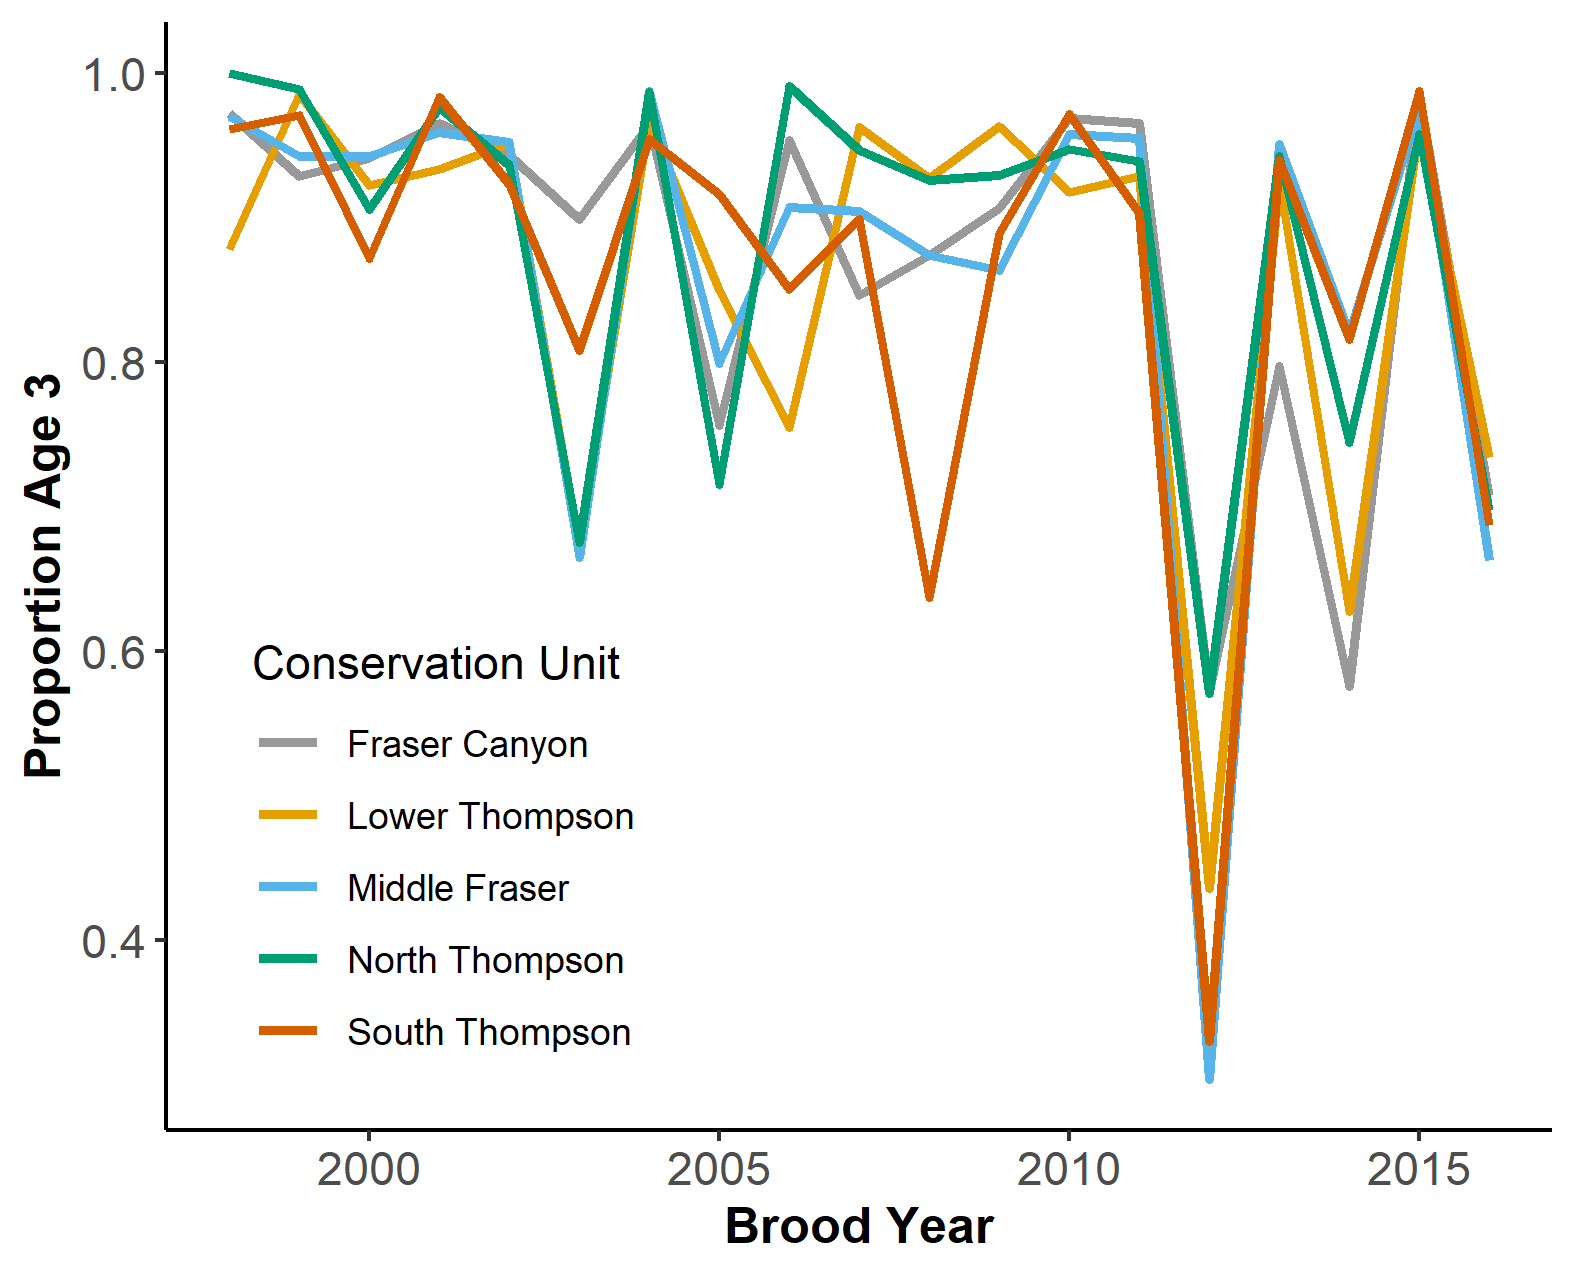
\includegraphics[width=0.5\linewidth]{figure/coho-ObsAgeProp-byCU}}{Figure \ref{fig:coho-ageProp}} 

}

\caption{Proportion of recruits returning at age 3 for 1998 - 2016 brood years. Only two age classes (age 3 and age 4) are present in the age structure, so the proportion of recruits returning at age 4 will account for the remainder of returns in each year.}\label{fig:coho-ageProp}
\end{figure}
\linebreak

\textbf{\emph{Covariance in exploitation}}

We assumed an average exploitation rate of 12.5\% for all CUs in forward projections based on average historical values, with common interannual variability in exploitation rates due to shared fishery impacts among CUs each year. Interannual variability in exploitation rates was assumed to be beta distributed (constrained between 0 and 1), with the standard deviation of the beta distribution parameterized from estimated exploitation rates for 1998 - 2016 brood years. The corresponding coefficient of variation (CV) for interannual variability was 0.44.

Exploitation rates for Interior Fraser Coho are only available at the SMU-level due to limited coded-wire indicator stocks (1-2 CUs with indicators / year) and variation in which indicator stocks were operational in a given year. As a result, empirically-based estimates of among-CU variability in exploitation rates are not available. However, there are reasons to expect exploitation rates to vary among CUs in a given year, including differences in freshwater fisheries. We assumed that CU-specific variability in exploitation rates was half the common (SMU-level) interannual variability (CV=0.22), and varied this in sensitivity analyses from 0 and 0.44 to cover plausible bounds. Varying assumptions about variability in exploitation among CUs between CV = 0 and 0.44 in forward projections did not impact the distribution of correlations in spawner abundances in the projections (results not shown).
\begin{longtable}[]{p{3.7cm} p{5cm} p{6.3cm}}
\caption{Parameters used for CU-specific projections of Interior Fraser Coho population dynamics.}\\
\hline
Parameter & Value & Source \\ 
\hline
\endhead
\hline
 Ricker Parameters ($\alpha$, $\beta$, $\gamma$,$\sigma$)  &  CU-specific (Appendix E) & Drawn from joint posterior from MCMC model fit to 1998-2016 brood years
\\\\

Smolt-to-adult marine survival rate (all CUs) & Drawn from Lognormal(-4.83, 1.21), bound between [-9.21, -3.32]
 & Estimated from annual marine survival rate estimates from brood years 1998 - 2016, with bounds set at lowest and highest observations
\\\\  

 Among-CU variability in marine survival coefficient $\gamma$  &  $\sigma_{\gamma}$ = 0 (all CUs the same) & Assumed value when fitting models. Varied between 0 and 0.09 in sensitivity analyses
\\\\

 Ave age proportions at maturity (ages 3, 4) &  MiddleFR, LThomp, SThomp = (0.86,0.14) , FRCanyon = (0.87, 0.13), NThomp = (0.88, 0.12) & Estimated from time-series of proportions of recruits at age
 \\\\  

 Interannual variability in age proportions (tau from multivariate logistic distribution)  & MiddleFR, NThomp, SThomp = 1.0, LThomp = 0.9, FRCanyon = 0.8 & Estimated from time-series of ppns of recruits at age. \\\\

 Average exploitation rate & 0.125 & Estimated from annual exploitation rate estimates from brood years 1998 - 2016. Varied in sensitivity analyses (0.05 - 0.35).
 \\\\

Interannual variability in exploitation rates & CV = 0.442  & Estimated from annual exploitation rate estimates from brood years 1998 - 2016. Assumed to be beta distributed, constrained between 0-1.
\\\\

Variability in exploitation rates among CUs & CV = 0.221 & Assumed to be half of interannual variability. Varied in a sensitivity analysis (0-0.442).
\\\\ 

Initial abundances  & CU-specific & Abundance initialized using spawner-recruit time series
\\\\

Extirpation threshold &  2 & Mating constraint \\
\hline
\label{tab:coho-BaseProjectPars}
\end{longtable}
\hypertarget{results-2}{%
\subsubsection{Results}\label{results-2}}

\textbf{\emph{LRP Estimates}}

Aggregate abundance-based LRPs estimated using the Ricker model as a basis for forward projections were lower than those obtained when the Ricker\_priorCap model was used, regardless of which probability threshold was used to derive the LRP (Figure~\ref{fig:coho-projLRPCurveByOM}; Table~\ref{tab:projectedLRPs2020}). This result is similar to the logistic regression-based LRPs, where LRPs derived using \(S_{gen}\) estimates from the Ricker\_priorCap model were higher due to higher \(S_{gen}\) values. The projected curve showing the probability of all CUs being above \(S_{gen}\) was more gradual and further to the right for the Ricker\_priorCap model compared to the base Ricker model (Figure~\ref{fig:coho-projLRPCurveByOM}). When projection outputs from both stock recruit model formulations were combined prior to binning in order to create a model-averaged scenario (with equal weight assigned to both scenarios), the resulting probability curve was mid-way between the curves from the two individual models. In all cases, projected curves had higher scatter with increasing aggregate abundance, such that LRP estimates at probability thresholds of p = 0.90 and p = 0.99 were unstable.
\begin{figure}[htb]

{\centering \pdftooltip{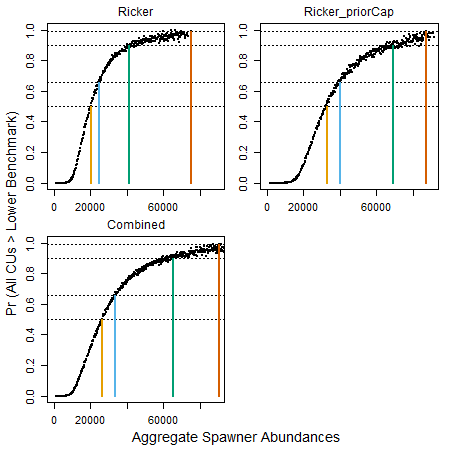
\includegraphics[width=0.5\linewidth]{figure/coho-projLRPCurve-byOM}}{Figure \ref{fig:coho-projLRPCurveByOM}} 

}

\caption{Probability of all CUs being above their lower benchmark of Sgen along a gradient in aggregate abundances within bins of 200 fish for two different stock recruit model options (Ricker and Ricker\_priorCap) as well as a model averaged case (Combined) in which results from both stock recruit models were equally weighted. Results are derived from projections over 30 years and 20,000 MC Trials. Each dot is the proportion of MC trials where all CUs were > lower benchmarks. Candidate LRPs at p=0.5 (yellow) and p=0.66 (blue), 0.90 (green), and 0.99 (orange) are highlighted.}\label{fig:coho-projLRPCurveByOM}
\end{figure}
\begin{longtable}[]{@{}
  >{\raggedright\arraybackslash}p{(\columnwidth - 6\tabcolsep) * \real{0.19}}
  >{\raggedright\arraybackslash}p{(\columnwidth - 6\tabcolsep) * \real{0.25}}
  >{\raggedright\arraybackslash}p{(\columnwidth - 6\tabcolsep) * \real{0.28}}
  >{\raggedright\arraybackslash}p{(\columnwidth - 6\tabcolsep) * \real{0.28}}@{}}
\caption{\label{tab:projectedLRPs2020} Projection-based LRPs from forward projections under two different stock recruit model options (Ricker and Ricker\textbackslash\_priorCap), as well as a model averaged case (Combined) in which results from both stock recruit models were equally weighted. For each probability level, the LRP estimate represents that probability that all CUs will be above their lower benchmark of \(S_{gen}\).}\tabularnewline
\toprule
\begin{minipage}[b]{\linewidth}\raggedright
Probability
\end{minipage} & \begin{minipage}[b]{\linewidth}\raggedright
Ricker
\end{minipage} & \begin{minipage}[b]{\linewidth}\raggedright
Ricker\_priorCap
\end{minipage} & \begin{minipage}[b]{\linewidth}\raggedright
Combined
\end{minipage} \\
\midrule
\endfirsthead
\toprule
\begin{minipage}[b]{\linewidth}\raggedright
Probability
\end{minipage} & \begin{minipage}[b]{\linewidth}\raggedright
Ricker
\end{minipage} & \begin{minipage}[b]{\linewidth}\raggedright
Ricker\_priorCap
\end{minipage} & \begin{minipage}[b]{\linewidth}\raggedright
Combined
\end{minipage} \\
\midrule
\endhead
50\% & 20,100 & 32,700 & 26,500 \\
66\% & 24,900 & 40,100 & 33,500 \\
90\% & 41,100 & 68,900 & 65,300 \\
99\% & 75,100 & 87,300 & 83,500 \\
\bottomrule
\end{longtable}
Generational average spawning abundance (based on a 3-year geometric mean) remained above the projection-based LRP derived using the Ricker model with a probability threshold of p = 0.5 for most years between 2000 and 2020. There were two years in which aggregate spawning abundance dropping below the LRP: 2006 and 2007 (Figure @ref:fig(coho-AggEscpSeries-wProjLRP). In comparison, when projection-based LRPs were derived using the Ricker\_priorCap model with p = 0.5, aggregate spawning abundance remained below the LRP for 11 out of the 21 years.
\begin{figure}[htb]

{\centering \pdftooltip{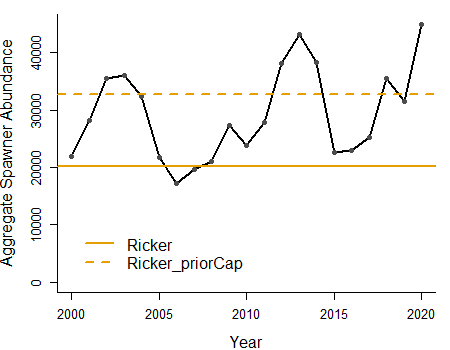
\includegraphics[width=0.6\linewidth]{figure/coho-EscpSeries-wProjLRP}}{Figure \ref{fig:coho-AggEscpSeries-wProjLRP}} 

}

\caption{Three-year geometric mean of aggregate spawning abundance for the Interior Fraser Coho SMU (black line) relative to projection-based LRP estimates using two different stock recruitment model formulations, Ricker and Ricker\_priorCap, with a probability threshold of p=0.5. Forward projections used to estimate reference points were parameterized using available 1998-2020 time series under base model assumptions.}\label{fig:coho-AggEscpSeries-wProjLRP}
\end{figure}
\linebreak

\textbf{\emph{Sensitivity Analyses}}

Increasing \(\sigma_{\gamma}\), which corresponded with reduced between-CU correlation in spawner abundances over time (Figure~\ref{fig:coho-sigGammaCorrelation}), resulted in a flattening of the projected relationship between aggregate spawer abundances and the probability of all CUs being above their lower benchmarks. LRP estimates corresponding to a given probability threshold increased as \(\sigma_{\gamma}\) increased as curves shifted to the right and became more gradual (i.e., less steep). For the two highest \(\sigma_{\gamma}\) scenarios examined (\(\sigma_{\gamma}\)=0.0675 and 0.09), a 99\% probability of all CUs being above their lower \(S_{gen}\) benchmark was never achieved.
\begin{figure}[htb]

{\centering \pdftooltip{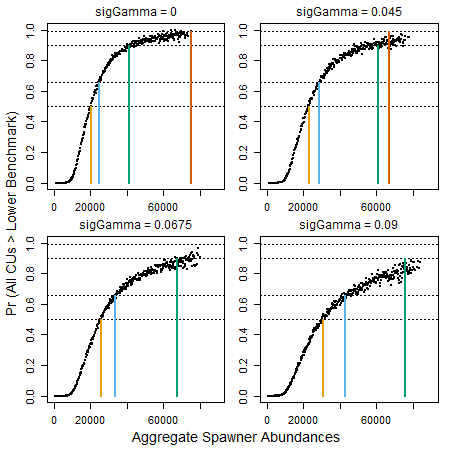
\includegraphics[width=0.6\linewidth]{figure/coho-projLRPCurve-bySigGamma}}{Figure \ref{fig:coho-projLRPCurve-bySigGamma}} 

}

\caption{Probability of all CUs being above their lower benchmark of Sgen along a gradient in aggregate abundances (within bins of 200 fish) for alternative scenarios about the value of sigGamma. The baseline value used for forward projections was sigGamma = 0. Results are derived from projections over 30 years and 20,000 MC Trials. Each dot is the proportion of MC trials where all CUs were > Sgen.  Candidate LRPs at p=0.5 (yellow) and p=0.66 (blue), 0.90 (green), and 0.99 (orange) are highlighted.}\label{fig:coho-projLRPCurve-bySigGamma}
\end{figure}
Increasing the average exploitation rate used in forward projections also led to a shift in projected curves to the right; however, the shift was more gradual over the range of exploitation rate scenarios we considered than the effect of increasing \(\sigma_{\gamma}\) (Figure~\ref{fig:coho-projLRPCurve-byER}). The effect of increasing exploitation rates was smallest at low probability thresholds. At p = 0.5, the LRP differed by 400 fish between the ER = 2.5\% and ER = 12.5\% scenarios (range = 19,700 - 21,000), and by \textless{} 4000 fish among all four scenarios (range = 19,700 - 24,000). Differences were much larger among the four exploitation rate levels examined for the p = 0.90 threshold. When the average exploitation rate was set at 22.5\% or 32.5\%, aggregate abundances barely exceeded 60,000 fish, and it was not possible to achieve a 99\% probability of all CUs being above their lower \(S_{gen}\) benchmarks.
\begin{figure}[htb]

{\centering \pdftooltip{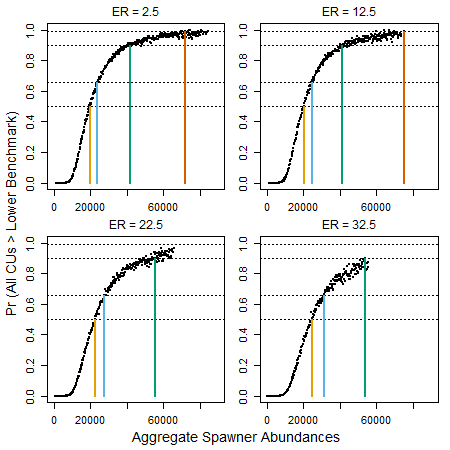
\includegraphics[width=0.6\linewidth]{figure/coho-projLRPCurve-byER}}{Figure \ref{fig:coho-projLRPCurve-byER}} 

}

\caption{Probability of all CUs being above their lower benchmark of Sgen along a gradient in aggregate abundances (within bins of 200 fish) for alternative scenarios about average exploitation rates (ER) in forward projections. The baseline value used for forward projections was ER = 12.5\%. Results are derived from projections over 30 years and 20,000 MC Trials. Each dot is the proportion of MC trials where all CUs were > Sgen.  Candidate LRPs at p=0.5 (yellow) and p=0.66 (blue), 0.90 (green), and 0.99 (orange) are highlighted.}\label{fig:coho-projLRPCurve-byER}
\end{figure}
\hypertarget{historical-evaluation-of-status-across-lrp-methods}{%
\subsection{HISTORICAL EVALUATION OF STATUS ACROSS LRP METHODS}\label{historical-evaluation-of-status-across-lrp-methods}}

We compared annual estimates of SMU status relative to LRPs for the range of LRP estimation options considered in this case study (Figure~\ref{fig:coho-statusPlot-withBars}). For all aggregate abundance-based LRPs, we used LRPs estimated using a probability threshold of p = 0.5 (i.e., a 50\% probability that all CUs would have status above their lower benchmark). We used the following labelling convention when comparing historical status estimates across LRP estimation methods: \emph{``Metric''~: ``LRP Method''~: ``CU Status Method''}. `Metric' refers to the choice of whether to base an LRP on the proportion of CUs above `poor' CU status (Prop) or on aggregate SMU-level abundance (Abund). The `LRP' method only applies to aggregate-abundance based LRPs, for which is can be logistic regression (Logistic) or projection-based (Proj). Finally, the `CU Status Method' can be based on the rapid multidimensional scanning tool in in which CU abundance-based benchmarks are based on one of the two Ricker models (Multidim-Ricker or Multidim-priorCap). Or, when only a single benchmark is used to characterize CU status, it can be based on \(S_{gen}\) estimated from one of the two Ricker models (Sgen-Ricker or Sgen-priorCap) or the IFCRT target (IFCRT). For example, when referring to an aggregate abundance-based LRP that is estimated via a logistic regression fit to historical CU status, with CU status estimated relative to \(S_{gen}\) from the base Ricker model, we label it as ``Abund: Logistic: Sgen\_Ricker.''

We show historical results for two types of proportional LRP methods: one that uses the proportion of CUs with rapid multidimensional status \textgreater{} red (e.g., Prop: Multidim-Ricker) and one that uses the proportion of CUs with abundance \textgreater{} Sgen (e.g., Prop: Sgen-Ricker). Holt et al.~(in review) recommend that the multidimensional approach should be used to assess status; however, we show results for the single metric \(S_{gen}\) approach here to demonstrate how the two approaches differ. This comparison is of interest because our aggregate abundance-based LRPs use status estimates based on a single metric rather than the multidimensional status estimates.

In addition to the LRP estimation methods presented so far in this case study, we include the full WSP assessment that was conducted in 2014 as an option for estimating CU status for use in a proportion-based LRP. We label this case ``Prop~: WSP-2014.'' SMU status would have been assessed as being above the LRP at this time as all CUs were assessed as amber or green.

In general, estimated LRP breaches coincided with low points in the aggregate abundance time series (2000, 2005 - 2006 and 2015-2017). However, there were differences among methods in the years that SMU status was estimated to be below the LRP, as well as a few methods for which status was never estimated to be below the LRP (Prop: Sgen-Ricker, Abund: Logistic: Sgen-Ricker, Abund: Logistic: IFCRT).

Comparison of SMU status estimates over time for all LRP estimation methods that used \(S_{gen}\) estimates from the base Ricker model (first group of four methods in Figure~\ref{fig:coho-statusPlot-withBars}), showed that the LRP was only breached in years 2015-2017 under the Prop: Multidim-Ricker method. The other three Ricker methods estimated status to remain above the LRP over this period. The latter three methods are similar in that they all assess CU status based on a direct comparison of CU-level abundance to \(S_{gen}\). In contrast, the decision tree for the rapid multidimensional scanning tool includes a step in which CU status is designated as `red' anytime the generational mean spawning abundance drops below 1500 spawners (Figure~\ref{fig:decision-tree}). Because estimated \(S_{gen}\) is less than 1500 spawners for the Fraser Canyon CU, it is possible for the criteria of \textless1500 spawners in a CU to be breached even though abundance remains above \(S_{gen}\). This situation occurs for this CU in 2015-2017. Therefore, LRP methods that use the rapid multi-dimensional scanning tool to characterize CU status can be more precautionary than methods that rely on a single \(S_{gen}\) benchmark.

In the years 2005-2006, SMU status estimates from the `Abund: Proj: Sgen-Ricker' method fell below the LRP, while the other two Sgen-Ricker methods did not. Declines in aggregate SMU abundance in 2005-2006 were driven by declines in the four larger CUs (which, still remained above their individual \(S_{gen}\) estimates). Declines in the lower abundance Fraser Canyon CU were not as drastic. As a result, while SMU-level aggregate abundance dropped below the abundance-based LRP, the Fraser Canyon CU that triggered `red' status in 2015-2017 remained above 1500 spawners and did not trigger the Prop: Multidim-Ricker method . The aggregate abundance-based LRP from the `Abund: Proj: Sgen-Ricker' estimation method was higher than that from the `Abund: Logistic: Sgen-Ricker,' so only the former method triggered an LRP breach.

When the Ricker-priorCap model was used to estimate \(S_{gen}\) instead of the base Ricker model, both \(S_{gen}\) and LRP estimates were higher than under the base Ricker model formulation. This in turn resulted in more frequent LRP breaches when the Ricker-priorCap model was used (see second group of four methods in Figure~\ref{fig:coho-statusPlot-withBars}) compared to when the base Ricker model was used. Among the `priorCap' methods, status was most frequently estimated to be below the LRP when the `Abund: Proj:Sgen-priorCap' method was used; for this method, the LRP was triggered in 13 out of the 21 years between 2000 and 2020. In comparison, the LRP was triggered in 8, 7, and 5 of the 21 years for the `Abund: Proj:Sgen-Ricker,' `Prop: Multidim-priorCap,' and `Prop: Sgen-priorCap' methods, respectively. LRP estimates based on the proportional LRPs estimated using the rapid multidimensional scanning tool were therefore the least precautionary of the thee priorCap methods.

Finally, SMU status remained above the LRP in all years under the Abund: Logistic: IFCRT method. Because the aggregate abundance-based LRP estimated using this method was similar to that of the Abund: Logistic: Sgen-Ricker (17,515 and 15,395 spawners, respectively), performance for these methods was similar. In comparison, the aggregate abundance-based LRP estimated using a logistic regression combined with the Ricker-priorCap model (Abund: Logistic: Sgen-priorCap) was higher (25,677 spawners).
\begin{figure}[htb]

{\centering \pdftooltip{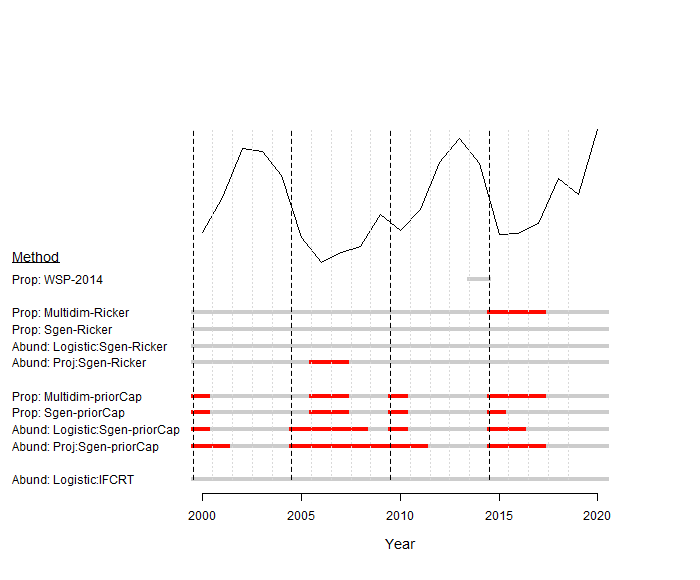
\includegraphics[width=0.8\linewidth]{figure/coho-statusPlot_withBars2020}}{Figure \ref{fig:coho-statusPlot-withBars}} 

}

\caption{Historical evaluation of status relative to LRP options considered for Interior Fraser Coho. The black line shows the 2000-2020 generational mean aggregate spawning abundance to the SMU. Red bars indicate years in which SMU status would have been assessed as being below the LRP. Estimates of Sgen benchmarks and aggregate abundance-based LRPs were based on data available up to 2020}\label{fig:coho-statusPlot-withBars}
\end{figure}
\hypertarget{discussion}{%
\subsection{DISCUSSION}\label{discussion}}

(Still in rough note form)

Discussion topic 1: What are the unique characteristics of this case study that can inform the development of guidelines
\begin{itemize}

\item
  Data rich SMU; while the number of years of data are limited, full SR time series are available for all 5 CUs. These have previously been used to develop forward simulations for individual CUs within the SMU.
\item
  Long history of using aggregate abundance-based recovery targets and fisheries reference points that were developed based on an underlying relationship between aggregate abundance and the distribution of abundance among sub-populations and CUs. As a result, it was well suited to looking at the application of aggregate abundance-based LRPs, as well as how they compared historically to the preferred proportional approach.
\end{itemize}
Discussion topic 2: How well do aggregate abundance-based LRPs perform retrospectively compared to proportional LRPs?
\begin{itemize}
\item
  The abundance-based methods we considered often matched the proportional methods in a historical comparison of SMU status relative to LRPs. For a given assumption about SR model structure, LRPs tended to be triggered in similar periods of times under the aggregate abundance-based and proportional options; however, there were some differences.
\item
  Our results highlight the complexities in predicting how well aggregate abundance-based LRPs will do at tracking proportion-based LRPs. For example, when estimates of Sgen were obtained using the base Ricker model, proportion-based LRPs using rapid multidimensional status were more precautionary than the two aggregate abundance-based LRP options; especially in years 2015-2017. This result is partially a function of the different methods used to estimate CU status (rapid multidiensional scanning tool vs.~single \(S_{gen}\) metric) rather than the choice of proportion vs aggregate abundance approach. When aggregate abundance-based LRPs are compared to proportion-based LRPs using a single \(S_{gen}\) metric, they are better aligned over this period. This result occurs because under the multidimensional approach, CUs can be above Sgen but still assessed as red status when their Sgen estimates are \textless{} 1500 spawners.
\item
  In comparison, when estimates of Sgen were obtained using the Ricker\_priorCap model, which produced higher Sgen and LRP estimates than the Ricker model, both types of proportion-based LRPs were less precautionary than aggregate abundance-based LRPs. This result was especially pronounced when aggregate abundance-based LRPs were estimated using the projection-based LRP approach. LRP breaches using the multidimensional scanning tool with Ricker-priorCap estimates in earlier years (i.e., before 2015) were based CU abundance relative to \(S_{gen}\), meaning that the two proportional methods were aligned. There were however additional years in which aggregate abundance LRPs were triggered but neither proportional LRP was. This pattern occurred when aggregate abundance dropped below abundance-based LRPs, but all CUs remained above red status based on CU-level abundances all being greater than \(S_{gen}\). While this pattern occurred for both types of \(S_{gen}\) estimates (Ricker and Ricker-priorCap), it was more common for the Ricker-priorCap model.
\end{itemize}
Discussion topic 3: Importance of SR model choice in characterizing SMU status in all approaches.
\begin{itemize}

\item
  All methods (with the exception of IFCRT) relied heavily on assessment of CU status relative to Sgen. This is even true for the Prop methods using the rapid mutlidimensional scanning tool because the decision tree relies heavily on estimates of Sgen when available, which they are for Interior Fraser Coho.
\item
  As a result, the method used to estimate Sgen had a large impact on results. Sgen estimates tended to be higher for the Ricker\_priorCap model compared to the base Ricker model, which meant that LRPs were more frequently triggered under this formulation.
\item
  We considered alternative Ricker models for Interior Fraser Coho because previous analyses for this SMU have done so. Arbeider et al.~(2020) used a model averaging approach with 3 SR models equally weighted when assessing recovery potential (the base Ricker and Ricker\_priorCap models we used, as well as a third depensatory mortality version that we did not consider).
\item
  Implementation of LRPs when considerable uncertainty in underlying model structure exists will require methods to integrate estimates of LRP status over alternative model structures. We demonstrate one approach when using projection-based estimates of aggregate abundance-based LRPs, in which we combine projections under each SR model scenario before calculating the LRP. This approach is basically a model-average approach in which both scenarios are equally weighted. However, other methods of assigning weights among model are possible. For example \ldots. (TO DO: reference model selection / averaging papers from Carrie). In other cases, such at the proportional approach using WSP assessments or the multi-dimensional scanning tool, uncertainty in model structure may best be dealt with through expert opinion. For example, under the planned expert workshops that will be used to confirm rapid multidimensional status estimates, participants could be given two sets of status results based on two different Sgen models, and then be asked to converge on a single status estimate. (can we pers. comm. Sue Grant as a reference for this process?).
\end{itemize}
Discussion topic 4: What was learned from retrospective analysis of logistic regression-based methods?
\begin{itemize}

\item
  Retrospective analyses of logistic regression-based LRP options showed that LRPs were sensitive to data availability. 2015 was the first year that that regression-based LRPs could be estimated, indicating that at least 18 years of data were required. (Although, note that the Logistic regression with the Base Ricker model could not estimate an LRP until 2017, so required 20 years of data). However, slight shifts in Sgen estimates in some years meant that logistic models were sometimes unable to converge on a solution even with more data.
\item
  For years in which LRPs could be estimated, LRP estimates did vary over time; especially when Sgen was estimated each year within an integrated modelling framework. LRP estimates were more stable when CU status was based on the IFCRT recovery target of at least half of all sub-populations within a CU having more than 1000 fish. This result is likely because CU-level SR parameters and lower benchmarks in a given historic year were not changing annually in the same way the did in the integrated Sgen-logistic regression model fits.
\item
  Missing data scenarios, in which 1 or 2 CUs were removed from the data set, highlighted limitations in the ability of the logistic regression models to converge on a solution given small changes in the pattern of `successes' and `failures' in the data used as inputs to the logistic regression. Estimates of aggregate SMU status, characterized as generational mean escapement / LRP, were also sensitive to the combination of CUs used. Removal of one or two influencial CUs often resulted in very different characterizations of CU status.
\item
  Taken together, these retrospective results highlight that caution should be used when applying logistic regression-based LRPs. While they did provide similar estimates of SMU status as proportion-based methods using the rapid multidimesional scanning tool for several (but not all) years in the historical comparison, they were sensitive to reductions in data availability. For the specific case of Interior Fraser Coho, retrospective performance may improve in the future as more data becomes available to improve the statistical power of logistic regression fits.
\end{itemize}
Discussion topic 5: What we learned from sensitivity analysis of projection-based methods?
\begin{itemize}

\item
  Projection-based LRPs were higher, and therefore more precautionary, than logistic regression-based LRPs when forward projections were parameterized using base case parameters. Given that the estimation of logistic regression-based LRPs were sensitive to data availability, projection-based LRPs may provide more reliable estimates for cases in which population and fishery dynamics can be modelled.
\item
  Projection-based LRPs also have the advantage of being able to incorporate hypotheses about current population and / or fishery dynamics into forward projections, whereas logistic regression-based LRPs are constrained by conditions that have been previously experienced.
\item
  The sensitivity of projection-based LRPs to exploitation rate means that these LRPs are specific to the management context. In our Interior Fraser Coho projections, it made sense to set exploitation rates at the recent average as fishery restrictions since 1998 have maintained relatively stable harvest dynamics. In this case, the LRP represents the level of aggregate abundance that would be required to ensure all CUs were above Sgen given a specified fixed ER policy. If a decision was made to increase the exploitation rate, the LRP would also be increased accordingly to ensure that the underlying objective of all CUs above Sgen could be achieved. This pattern arises due to variability in productivity among CUs; when higher exploitation rates are applied, some low productivity CUs will require higher spawning abundances to ensure that they remain above Sgen. This effect is demonstrated in Appendix~\ref{app:ERsensitivity-appendix}. As a result, projection-based LRPs are not static measures of serious harm, as commonly developed for other stocks/species.
\item
  Projection-based LRPs were also sensitive to the level of co-variation in spawner abundances among CUs over time. Reductions in covariation resulted in increased LRP estimates. This pattern will result in more precautionary LRPs as the relationship between aggregate abundance and CU status weakens. Projected LRPs therefore have a built-in buffer that will help avoid the situation where aggregate abundance remains above the LRP despite several CUs having poor realized status.
\end{itemize}
\hypertarget{WCVIchinookChapter}{%
\section{CASE STUDY 2: WEST COAST VANCOUVER ISLAND CHINOOK}\label{WCVIchinookChapter}}

\hypertarget{context-1}{%
\subsection{CONTEXT}\label{context-1}}

The West Coast of Vancouver Island (WCVI) Chinook SMU is comprised of 3 CUs (\protect\hyperlink{ref-holtbyConservationUnitsPacific2007}{Holtby and Ciruna 2007}), 7 large inlets (or sounds), and 20 indicators stocks, which are stocks with relatively complete time-series and consistent observation methodology (Figure~\ref{fig:chinook-map}; Table~\ref{tab:chinook-Overview}, \protect\hyperlink{ref-riddellReview2001Chinook2002}{Riddell et al.} (\protect\hyperlink{ref-riddellReview2001Chinook2002}{2002})). Hatchery enhancement is an important component of many of these stocks. Hatcheries are a conservation tool for wild salmon populations and can increase the availability of fish for harvest, but they can also reduce wild genetic diversity and are considered a risk factor for the long-term sustainability of CUs (\protect\hyperlink{ref-withlerGeneticallyBasedTargets2018}{Withler et al. 2018}). Therefore only indicator stocks without significant enhancement were included in our analyses. Proportionate Natural Influence, PNI, is a metric of the genetic risk of hatcheries on natural populations, with values \textless{} 0.5 indicating Integrated-Hatchery populations where most fish are hatchery origin (\protect\hyperlink{ref-withlerGeneticallyBasedTargets2018}{Withler et al. 2018}). Only stocks with PNI values \(\geqslant\) 0.5 were included in the development of LRPs and assessment against those LRPs (J. Bokvist, pers. comm. DFO South Coast Stock Assessment).
\begin{figure}[htb]

{\centering \pdftooltip{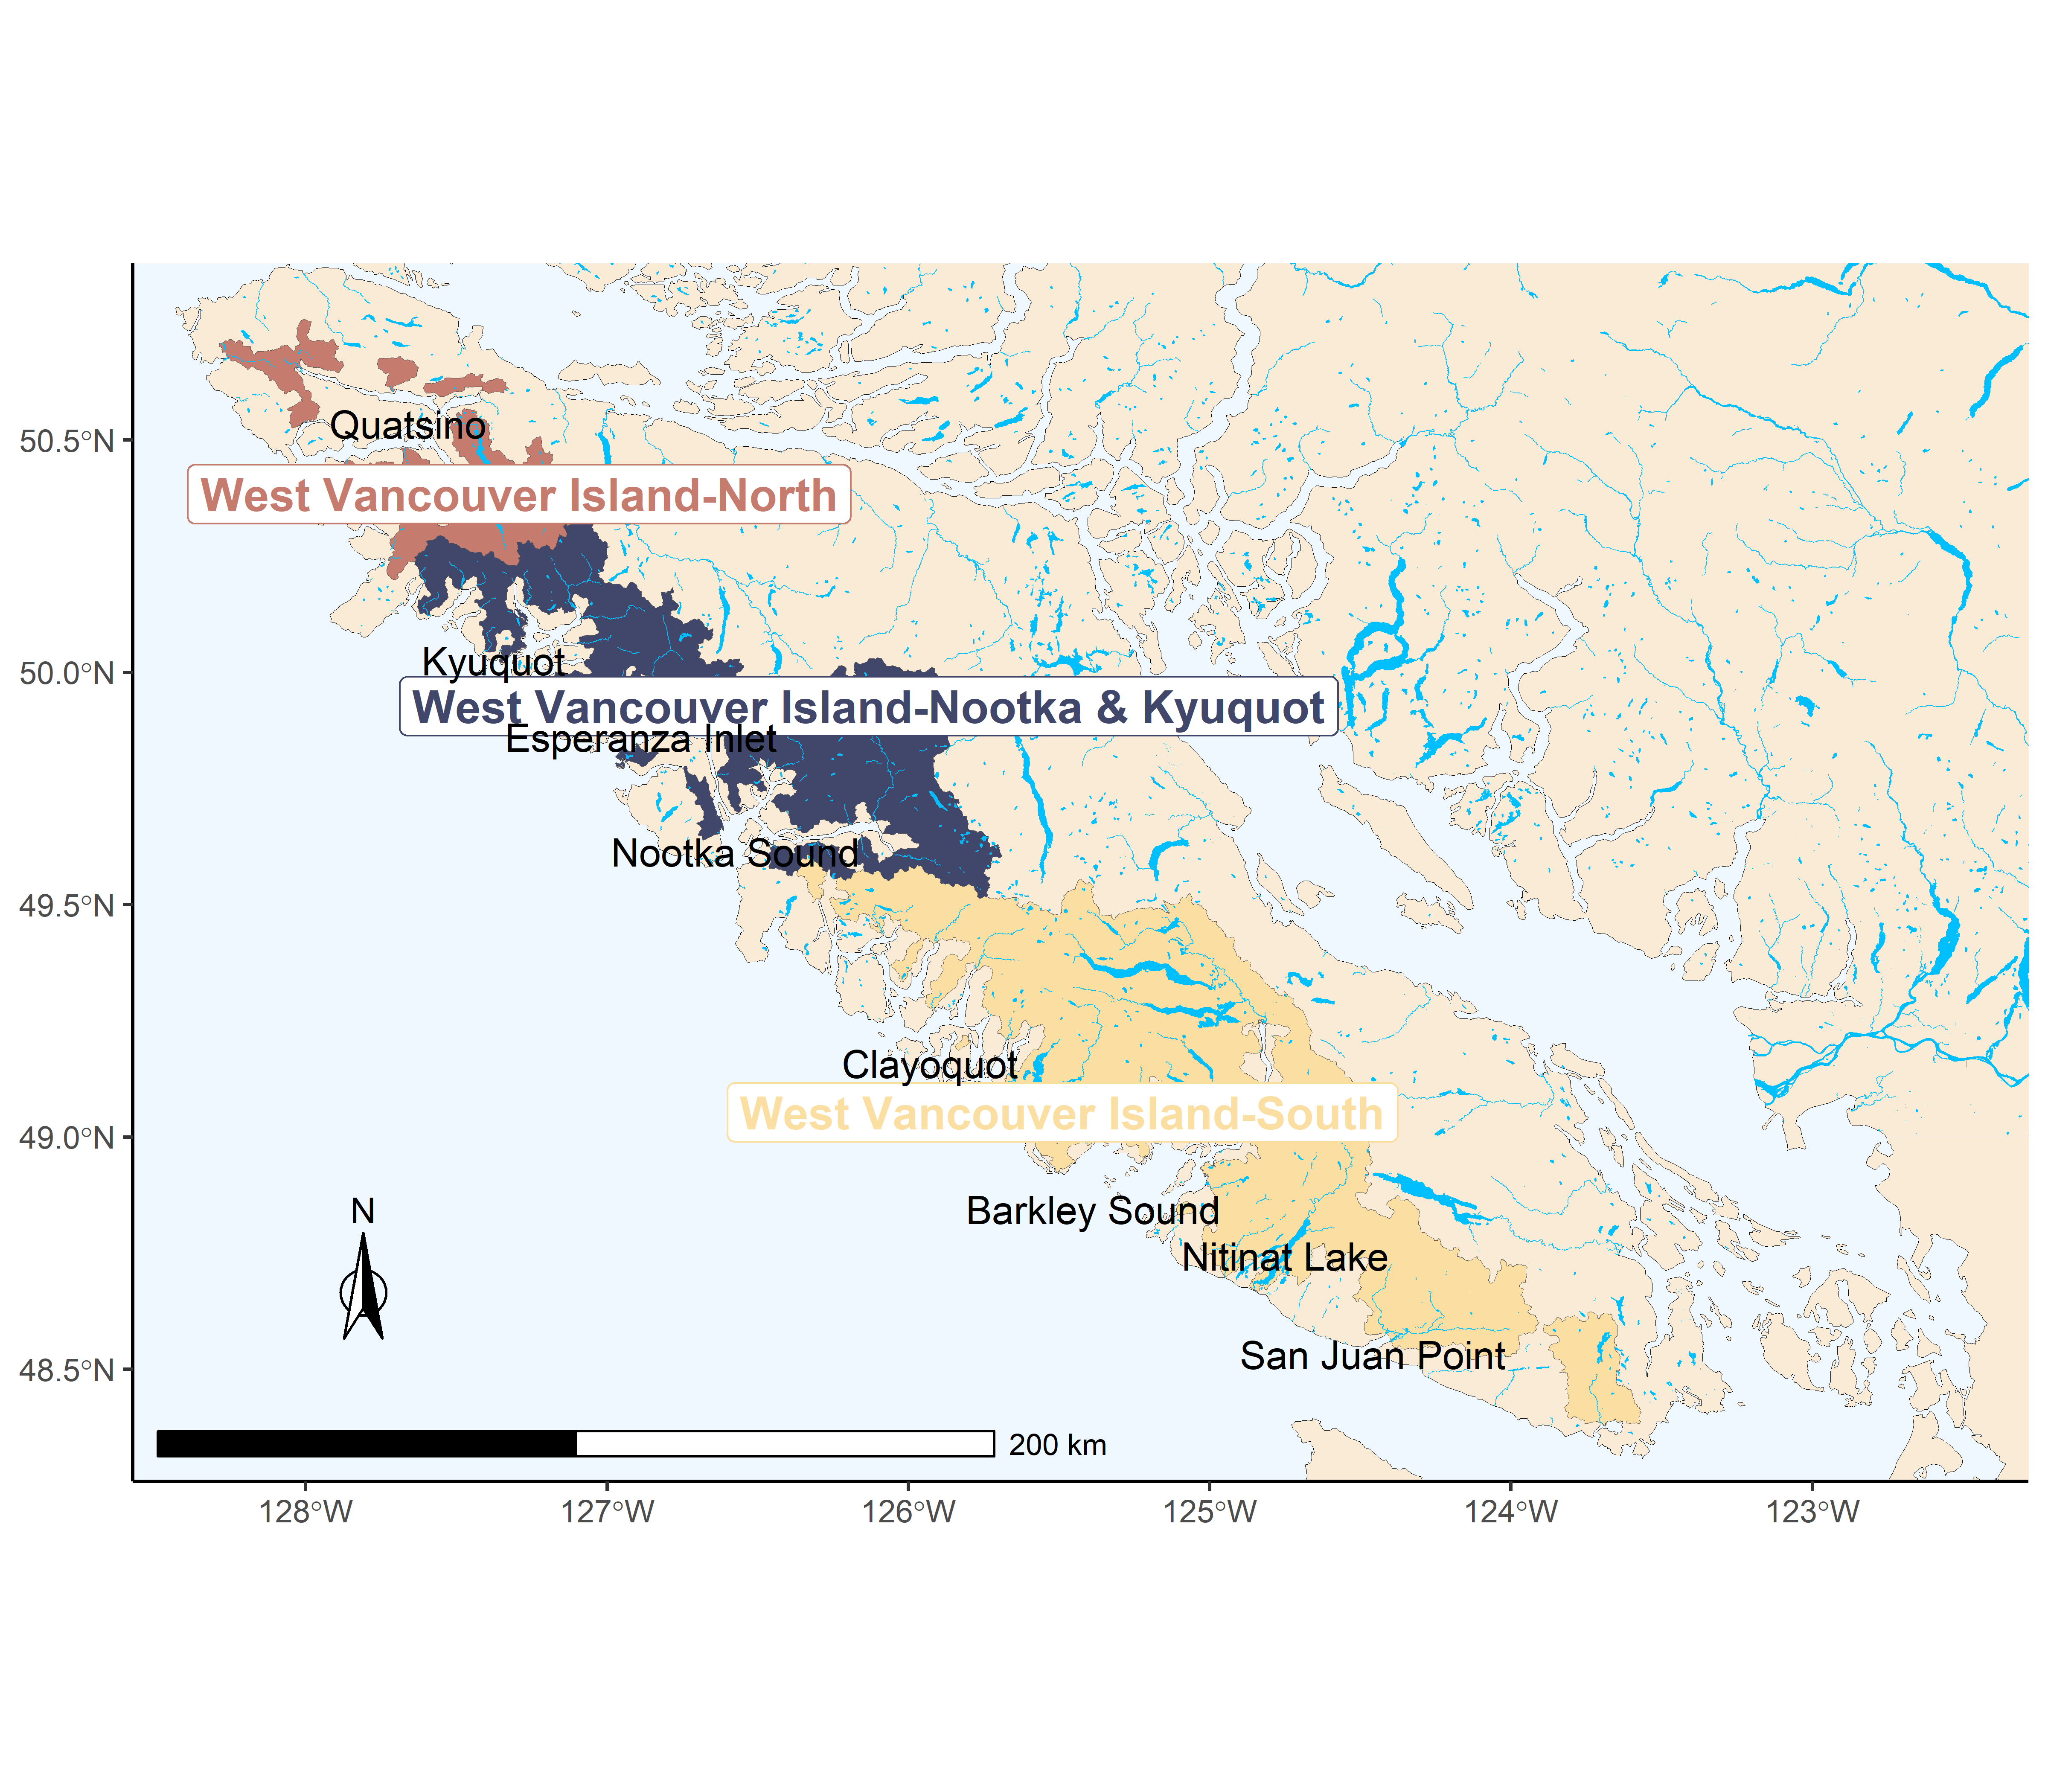
\includegraphics[width=6in]{figure/chinook-map}}{Figure \ref{fig:chinook-map}} 

}

\caption{Map of the WCVI Chinook SMU, component CUs (coloured red, blue, and yellow), and inlets (labelled in black- NAMES TO BE REVISED).}\label{fig:chinook-map}
\end{figure}
\renewcommand*{\arraystretch}{1.5}
\begin{table}[ht]
\centering
\caption{Overview of WCVI Chinook Stock Management Unit. Italics represent indicators with average PNI values < 0.5. Note, the inlets, San Juan and Nitinat do not contain indicator stocks with PNI < 0.5 and are not included in these analyses. WCVI is West Coast of Vancouver Island.}
\begin{tabular}{p{0.3\textwidth}p{0.2\textwidth}p{0.4\textwidth}}
\hline
CU       &  Inlets   & Indicators\\ 
\hline
WCVI-South (CK-31) & San Juan, Nitinat, Barkley, Clayoquot & \emph{San Juan}, \emph{Nitinat}, Nahmint , \emph{Sarita}, \emph{Somass}, Bedwell/Ursus , Megin , Moyeha , \emph{Tranquil} \\
WCVI-Nootka \& Kyuoquot (CK-32) & Nootka/Esperanza, Kyuquot & \emph{Burman}, \emph{Conuma}, \emph{Gold}, \emph{Leiner}, Tahsis, Zeballos, Artlish, Kaouk, Tahsish \\
WCVI-North (CK-33) &  Quatsino  & Cayeghle, Marble \\                     
\hline
\end{tabular}
\label{tab:chinook-Overview}
\end{table}
This SMU was included as a case study to demonstrate the development of LRPs under data limitations when stock-recruitment relationships are not available to develop stock-recruitment based benchmarks, but habitat-based benchmarks are, as is common for Chinook salmon in BC. WCVI Chinook is also included in the proposed first batch of major stocks for regulation under the Fish Stock provisions, necessitating the development of LRPs for this SMU.

Most Chinook in this SMU are `ocean type,' entering the ocean 1-3 months after emergence from spawning gravel (\protect\hyperlink{ref-dfoAssessmentWestCoast2012}{DFO 2012}). `Stream type' fish, those that stay in the river for one year after emergence, are rare. After entering the ocean, WCVI Chinook migrate into northern BC and southeast Alaska waters to rear for 2 to 7 years, returning to spawn predominantly at ages 4 and 5 (\protect\hyperlink{ref-dfoAssessmentWestCoast2012}{DFO 2012}).

\hypertarget{previous-assessments-1}{%
\subsubsection{Previous assessments}\label{previous-assessments-1}}

Two of the 3 CUs in this SMU, WCVI-South and WCVI-Nootka \& Kyuquot, were assessed as `red' status in an integrated Wild Salmon Policy assessment (\protect\hyperlink{ref-dfoIntegratedBiologicalStatus2016}{DFO 2016}). For these CUs, assessments were based on component stocks without hatchery enhancement within the most recent 12 years, omitting stocks with enhancement during that period. For WCVI-South, red status was based primarily on threats of genetic introgression from strays from nearby large-scale hatcheries. For WCVI-Nootka \& Kyuoquot, red status was based on a very low index of abundance for non-enhanced populations and threats of genetic introgression from strays from large-scale hatcheries. The third CU, WCVI-North, was not assessed by DFO in 2016 because all component stocks had some level of enhancement over the most recent 12 years (other metrics of hatchery enhancement, e.g., Proportionate Natural Influence or PNI were not considered). A list of indicator and non-indicator stocks within each CU is available in \protect\hyperlink{ref-brown2020SummaryAbundance2020}{Brown et al.} (\protect\hyperlink{ref-brown2020SummaryAbundance2020}{2020}).

WCVI Chinook was identified as a stock of concern in the 2021 Integrated Fisheries Management Plan, IFMP, for South Coast Salmon, and a rebuilding plan is under development (\protect\hyperlink{ref-dfoIntegratedFisheriesManagement2021}{DFO 2021a}). Poor marine survival rates for WCVI Chinook and low spawner levels over the past 2 decades are highlighted as reasons for conservation concern in the IFMP (\protect\hyperlink{ref-dfoIntegratedFisheriesManagement2021}{DFO 2021a p. 129}). A variety of management measures have been implemented to restrict harvest on WCVI Chinook and address these concerns, described in the IFMP (\protect\hyperlink{ref-dfoIntegratedFisheriesManagement2021}{DFO 2021a}).

Biological benchmarks have been estimated for WCVI indicator stocks using an empirical relationship between watershed area and common stock-recruitment biological benchmarks, spawner abundances at replacement, \(S_{REP}\), and \(S_{MSY}\), from a meta-analysis of 25 Chinook stocks across North America (\protect\hyperlink{ref-parkenHabitatbasedMethodsEstimate2006}{Parken et al. 2006}). Lack of rigorous recruitment data for WCVI Chinook stocks has precluded the use of stock-recruitment based benchmarks. For the development of LRPs for WCVI Chinook, the empirical relationship between watershed area and \(S_{REP}\) was re-estimated using a hierarchical Bayesian model (as in \protect\hyperlink{ref-liermannUsingAccessibleWatershed2010}{Liermann et al.} (\protect\hyperlink{ref-liermannUsingAccessibleWatershed2010}{2010})), and applied to inlets of WCVI Chinook (Appendix X, to be included).

Under Canada's Wild Salmon Policy, CUs are identified at a spatial scale that allows for long-term sustainability of the species (\protect\hyperlink{ref-holtbyConservationUnitsPacific2007}{Holtby and Ciruna 2007}). For WCVI Chinook, inlets nested within CUs are another important spatial scale of diversity for sustainability given geographic separation of spawning habitats among inlets and limited straying among inlets (D. McHugh pers. comm. DFO South Coast Stock Assessment). We used a hybrid approach that preserved CU-scale diversity, while also considering inlet-scale diversity. Specifically, LRPs were developed to preserve inlet-scale diversity within CUs. However, only 5 of the 7 inlets on the west coast of Vancouver Island contained indicators stock without significant hatchery influence. The lack of indicators without significant hatchery influence for inlets Nitinat and San Juan is due to large-scale hatcheries and infrequent monitoring of sites with natural spawning. Because the remaining 5 inlets with significant natural spawning are nested within the 3 WCVI Chinook CUs, preserving this inlet-scale biodiversity will also preserve CU-scale biodiversity required under the Wild Salmon Policy. Future analyses could limit LRP estimation to the scale of CUs or extend it to include all 7 inlets with additional natural indicators for Nitinat and San Juan, if they are developed.

\hypertarget{data}{%
\subsection{DATA}\label{data}}

\hypertarget{watershed-areas}{%
\subsubsection{Watershed Areas}\label{watershed-areas}}

To derive habitat-based benchmarks, watershed areas were updated for WCVI Chinook using methods described in \protect\hyperlink{ref-parkenHabitatbasedMethodsEstimate2006}{Parken et al.} (\protect\hyperlink{ref-parkenHabitatbasedMethodsEstimate2006}{2006}) by identifying 3rd order watershed areas that contain spawning habitat and omitting areas above obstacles to fish passage from the \href{https://catalogue.data.gov.bc.ca/dataset/provincial-obstacles-to-fish-passage}{Provincial Obstacles to Fish Passage database} (Appendix X, to be included). Only watershed areas for indicator stocks were included in the current analyses, and these watershed areas were then summed within inlets (Table~\ref{tab:chinook-WA}). In future analyses, watershed areas of all known spawning populations could be included (omitting areas above obstacles to fish passage) to derive habitat-based benchmarks on an absolute abundance scale. These benchmarks could be compared against total abundances to each inlet. This approach was not used as a base case because of large uncertainties in abundances of non-indicator stocks.
\begin{longtable}[]{@{}lr@{}}
\caption{\label{tab:chinook-WA}Sum of watershed areas for indicator stocks within inlets, km\textsuperscript{2}. Only indicator stocks that are not highly enhanced (i.e., PNI \textgreater{} 0.5) are included.}\tabularnewline
\toprule
Inlet & Watershed Area \\
\midrule
\endfirsthead
\toprule
Inlet & Watershed Area \\
\midrule
\endhead
Barkley & 42 \\
Clayoquot & 460 \\
Kyuquot & 336 \\
Nootka/Esperanza & 77 \\
Quatsino & 217 \\
\bottomrule
\end{longtable}
\hypertarget{spawner-abundances}{%
\subsubsection{Spawner Abundances}\label{spawner-abundances}}

Spawner abundances were provided for 20 WCVI indicators stocks, (D. Dosbon and D. McHugh pers .comm.; Table~\ref{tab:chinook-Overview}; Figure~\ref{fig:chinook-IndTimeSeries}). These time-series are compiled annually by DFO Area Staff for local and international assessment and management (e.g., \protect\hyperlink{ref-dfoWCVISalmonBulletin2021}{DFO} (\protect\hyperlink{ref-dfoWCVISalmonBulletin2021}{2021b})). Missing values were not infilled. In future work, infilled time-series of indicators within inlets (or CUs) could be developed to extend the available time-series.
\begin{figure}[htb]

{\centering \pdftooltip{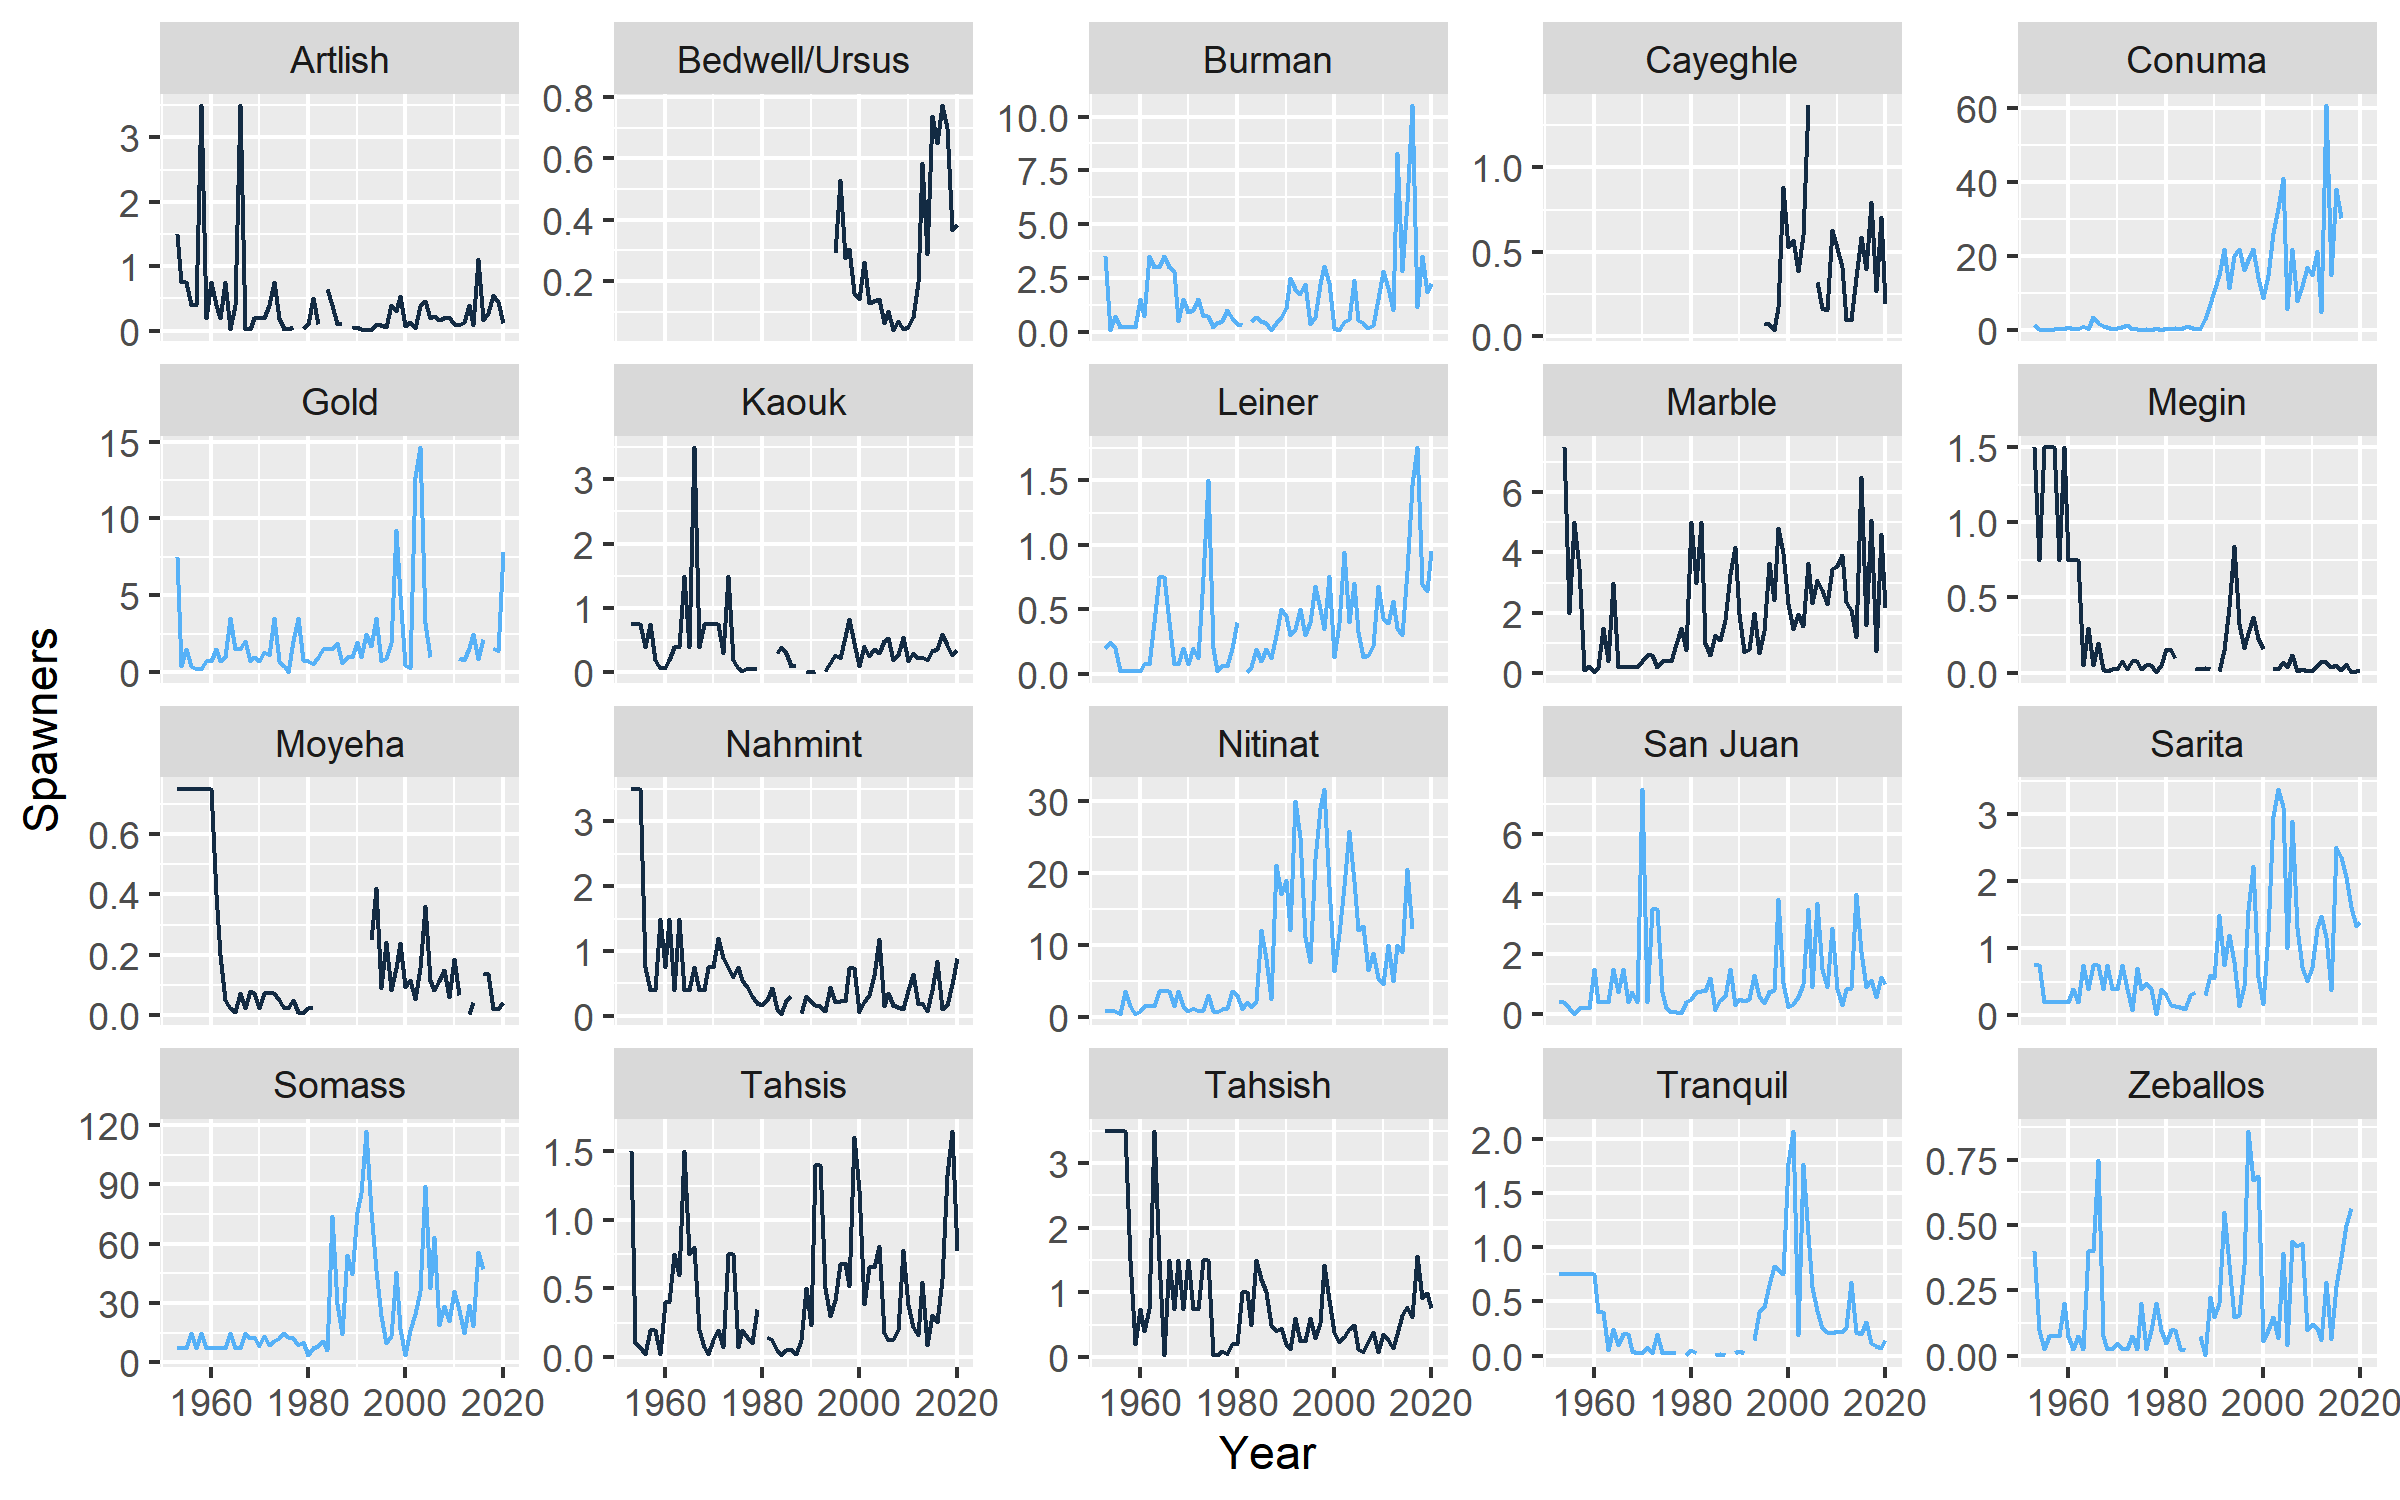
\includegraphics[width=6in]{figure/chinook-IndicatorTimeSeries}}{Figure \ref{fig:chinook-IndTimeSeries}} 

}

\caption{Time-series of spawner abundances by indicator stock. Dark blue time-series are indicator stocks with Proportionate Natural Index (PNI) values <= 0.5; light blue time-series are indicator stocks with PNI < 0.5, i.e., are highly enhanced.}\label{fig:chinook-IndTimeSeries}
\end{figure}
\hypertarget{proportionate-natural-influence-pni}{%
\subsubsection{Proportionate Natural Influence, PNI}\label{proportionate-natural-influence-pni}}

PNI values for 14 WCVI indicator stocks were provided to DFO South Coast Stock Assessment by DFO's Salmonid Enhancement Program (J. Bokvist, pers. comm. DFO South Coast Salmon Assessment). Stocks were considered significantly enhanced if average PNI values over available time-series were \textless{} 0.5, representing integrated-hatchery stocks where most fish are hatchery origin (\protect\hyperlink{ref-withlerGeneticallyBasedTargets2018}{Withler et al. 2018}). Thermal marking was used to identify the proportion of hatchery-origin spawners on the spawning grounds to derive PNI values. When data on thermal marking were not available; coded-wire tags (CWTs) were used to identify hatchery-origin spawners. Although Gold River had PNI values \textgreater{} 0.5 (0.52), most of the unmarked spawners are thought to be second generation (or descendants of) hatchery-origin fish from the Robertson Creek hatchery. There is no evidence of the original natural spawners in this system, so it was excluded from our analyses. Five of the remaining 6 indicator stocks without PNI data are not thought to be significantly enhanced, Cayeghle, Kaouk, Megin, Moyeha and Tasish (D. McHugh, pers. comm., DFO South Coast Stock Assessment). One indicator stock without PNI data, Tranquil, was considered significantly enhanced and was grouped with the PNI \textless0.5 stocks (D. McHugh, pers. comm., DFO South Coast Stock Assessment). Guidelines and methods for estimating PNI values are currently being documented by DFO's Salmonid Enhancement Program.

\hypertarget{proportion-of-cus}{%
\subsection{PROPORTION OF CUS}\label{proportion-of-cus}}

\hypertarget{methods-2}{%
\subsubsection{METHODS}\label{methods-2}}

\(S_{REP}\) values were derived from the watershed-area model adapted from \protect\hyperlink{ref-parkenHabitatbasedMethodsEstimate2006}{Parken et al.} (\protect\hyperlink{ref-parkenHabitatbasedMethodsEstimate2006}{2006}) (Appendix X, to be included). The Wild Salmon Policy lower benchmark on abundances, \(S_{gen}\), the spawner abundances required to achieve \(S_{MSY}\) within one generation without fishing under equilibrium conditions, was derived by optimizing the Ricker equation with recruitment set to \(S_{MSY}\).
\begin{equation}
  S_{MSY} = a * S_{gen}* e^{-b * S_{gen}}
   \label{eq:Sgen}
\end{equation}
where,
\begin{equation}
  b = \frac{\log(a)}{S_{REP}}
   \label{eq:ricB}
\end{equation}
\begin{equation}
  S_{MSY} = \frac{1 - W{e^{1-\log(a)}} } {b}
   \label{eq:SMSY}
\end{equation}
and \(a\) is recruits-per-spawner at low productivity. Ricker \(a\) values were approximated for WCVI Chinook from a life-stage model that partitioned survival across freshwater and marine life-stages for ocean-type chinook based on empirical data and expert opinion. Life-stage specific survival rates were then combined to derive an overall survival from spawners to recruitment (W. Luedke pers. comm. DFO South Coast Stock Assessment). Despite the relatively large uncertainties in the life-stage specific survival rates, this approach provides an approximation for productivity that is more realistic than the high estimate previously derived from the watershed-area model (\protect\hyperlink{ref-parkenHabitatbasedMethodsEstimate2006}{Parken et al. 2006}), (\textgreater7 recruits/spawner). From the life-stage model, mean \(\log(a)\) was estimated at \textasciitilde{} 1 (\textasciitilde{}\(a\)=2.72 recruits/spawner), with standard errors (1.96 SDs) +/- 0.5 (\(a\) ranging from 1.6 to 4.5), representing relatively large uncertainty in productivity. Bootstrapped confidence intervals in \(S_{gen}\) (Equation~\ref{eq:Sgen}) were estimated by repeated sampling from normal distributions of \(\log(S_{REP})\) and \(\log(a)\), with standard deviations in \(\log(S_{REP})\) derived from the watershed-area model. This method does not account for covariance between productivity and capacity typically found in stock-recruitment relationships, and will overestimate uncertainty in derived benchmarks.

Our approach to estimating \(S_{gen}\) differed from that of \protect\hyperlink{ref-parkenHabitatbasedMethodsEstimate2006}{Parken et al.} (\protect\hyperlink{ref-parkenHabitatbasedMethodsEstimate2006}{2006}), because we derived productivity independently from the life-stage specific models, whereas \protect\hyperlink{ref-parkenHabitatbasedMethodsEstimate2006}{Parken et al.} (\protect\hyperlink{ref-parkenHabitatbasedMethodsEstimate2006}{2006}) estimated both \(S_{MSY}\) and \(S_{REP}\) from the watershed-area model thereby inferring mean estimates of productivity which were deemed unrealistically high for WCVI Chinook.
\begin{longtable}[]{@{}lrrrrrr@{}}
\caption{\label{tab:chinook-benchmarks}Benchmarks and boostrapped 95\% confidence intervals (labelled, lwr and upr) for five inlets, including only indicator stocks that are not highly enhanced.}\tabularnewline
\toprule
Stock or inlet & Sgen & Sgen.lwr & Sgen.upr & SREP & SREP.lwr & SREP.upr \\
\midrule
\endfirsthead
\toprule
Stock or inlet & Sgen & Sgen.lwr & Sgen.upr & SREP & SREP.lwr & SREP.upr \\
\midrule
\endhead
Barkley & 111 & 33 & 373 & 630 & 283 & 1277 \\
Clayoquot & 1390 & 399 & 3969 & 7265 & 4348 & 12556 \\
Kyuquot & 1050 & 234 & 2940 & 5333 & 2898 & 9375 \\
Nootka/Esperanza & 241 & 56 & 739 & 1205 & 572 & 2579 \\
Quatsino & 658 & 165 & 2073 & 3425 & 1744 & 6142 \\
\bottomrule
\end{longtable}
\begin{figure}[htb]

{\centering \pdftooltip{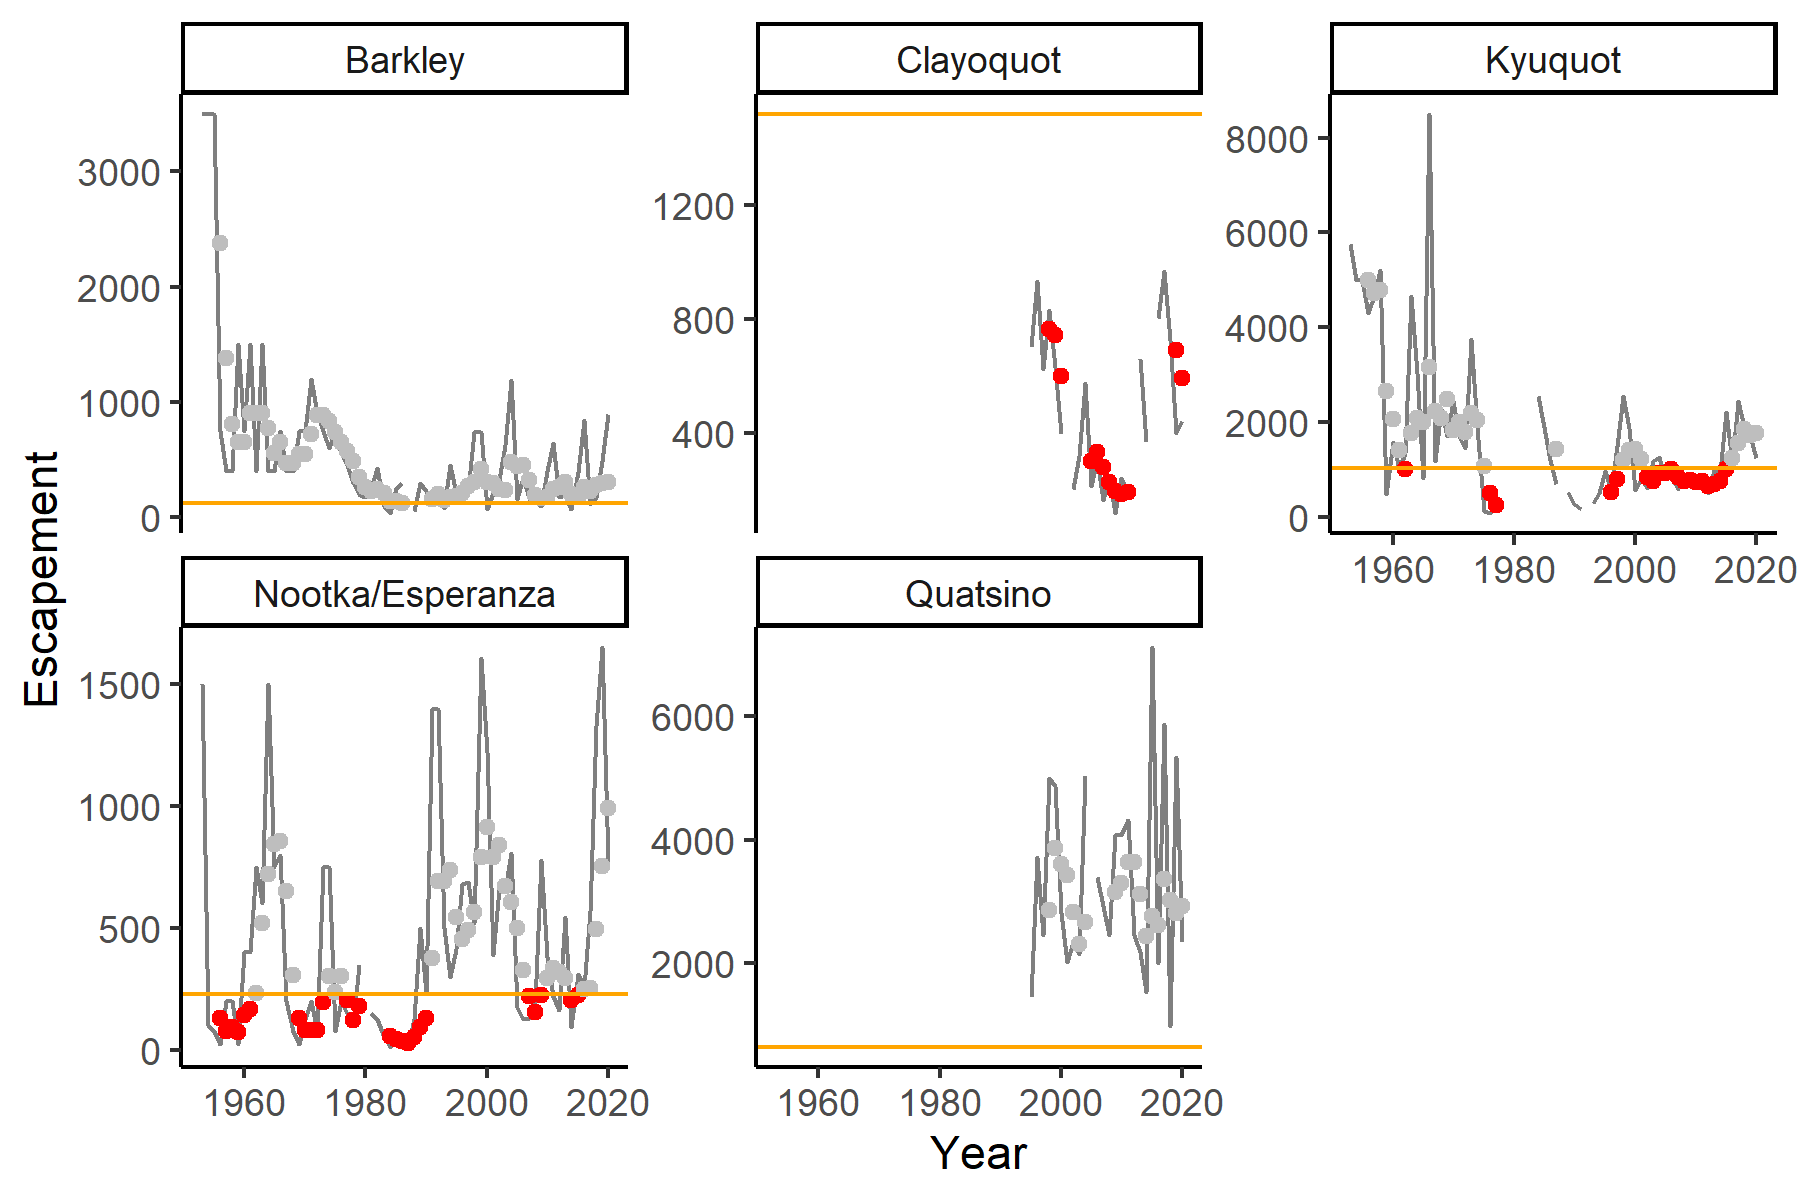
\includegraphics[width=6in]{figure/chinook-inlet-timeseries}}{Figure \ref{fig:chinook-InletTimeSeries}} 

}

\caption{Time-series of spawner abundances by inlet, including only indicators stocks that are not highly enhanced. Horizontal yellow line is Sgen and dots are generational geometric average spawner abundances coloured by red (below Sgen) and grey (above Sgen).}\label{fig:chinook-InletTimeSeries}
\end{figure}
The LRP on the proportion of CUs was identified as all 3 CUs containing inlets with current statuses exclusively above their lower benchmarks. For this SMU, serious harm was identified as any one inlet within each of the 3 CUs dropping below its lower benchmark or in the red zone under the Wild Salmon Policy. Because inlets are nested within CUs, this LRP accounts for the distribution of spawning within CUs. Status of inlets within CUs was identified in two ways: spawner abundances relative to \(S_{gen}\) and multi-dimensional status assessments developed by the DFO's State of the Salmon program (S. Grant. pers. comm. DFO Science; Figure~\ref{fig:decision-tree}).

\hypertarget{results-proportion-of-cus}{%
\subsubsection{RESULTS: PROPORTION OF CUs}\label{results-proportion-of-cus}}

In the most recent year with data, 2020, 4 of 5 inlets are above their abundance-based lower benchmark, \(S_{gen}\) (Figure~\ref{fig:chinook-InletTimeSeries}). Therefore, 2 of 3 CUs contain inlets with current statuses exclusively above their lower benchmarks. One CU, Southern Vancouver Island, contains an inlet, Clayoquot, with status that has been consistently below its lower benchmark throughout the available time-series. Therefore this SMU falls below the LRP of 3/3 CUs.

Using the multidimensional approach, the status was the same as for the abundance-based lower benchmarks. For this SMU, time-series of abundances for WCVI Chinook are not absolute (only indicator stocks are monitored consistently) and relative-abundance benchmarks can be identified (\(S_{gen}\) and \(S_{MSY}\)), and so according to the multidimensional decision tree (Figure~\ref{fig:decision-tree}, status is derived from abundance-based benchmarks as above. Therefore, similar to above, 2 of 3 CUs met the criteria of containing inlets with status above the red zone under the multi-dimensional approach, falling below the LRP of 3/3 CUs.

\hypertarget{aggregate-abundance-empirical-lrps}{%
\subsection{AGGREGATE-ABUNDANCE, EMPIRICAL LRPS}\label{aggregate-abundance-empirical-lrps}}

Empirical LRPs based on the probability of all component inlets (nested within CUs) being above their lower benchmarks could not be identified for WCVI Chinook because there are no years when all inlets were above their lower benchmark in the historical record (Figure~\ref{fig:chinook-InletTimeSeries}). In order to fit a logistic regression model to data, observations of successes (years when all inlets were \textgreater{} lower benchmarks) and failures (years when all inlets were not \textgreater{} lower benchmarks) are required. The estimation of empirical LRPs is limited to SMUs with historical records that demonstrate contrast in status over time.

\hypertarget{aggregate-abundance-projection-based-lrps}{%
\subsection{AGGREGATE-ABUNDANCE, PROJECTION-BASED LRPS}\label{aggregate-abundance-projection-based-lrps}}

\hypertarget{methods-3}{%
\subsubsection{METHODS}\label{methods-3}}

Projection-based LRPs were derived for WCVI Chinook by projecting inlet-specific population dynamics using the \texttt{samSim} modelling tool (Appendix~\ref{app:samsim-appendix}). We chose to project inlet-specific rather than CU-specific population dynamics to reflect the importance of the inlet scale of diversity for long-term sustainability of the SMU. Population dynamics and exploitation parameters were derived from a previously developed CU-specific run-reconstruction for WCVI Chinook based on spawner abundances and age compositions from indicator stocks, and exploitation rates from the Robertson Creek hatchery indicator stock (D. Dobson \& D. McHugh, pers. comm. DFO South Coast Stock Assessment). CU-specific parameters were applied across all component inlets. Inlet-specific capacities, or spawner abundances at replacement, were estimated from the watershed-area model (\protect\hyperlink{ref-parkenHabitatbasedMethodsEstimate2006}{Parken et al. 2006}) (Table~\ref{tab:chinook-WA}) and applied in projections of recruitment. The model was projected for 30 years from initial equilibrium abundances as recent abundance data is not available. Projections were summarized over 50,000 random Monte Carlo trials. A relatively large number of Monte Carlo trials was required for LRP estimation because the algorithm required a sufficient sample size within each 200-fish incremental bin of aggregate abundances along a range of realistic abundances (from near zero to capacity). Base-case parameters are provided in Table~\ref{tab:chinook-BaseCasePars}; sensitivity analyses from base case parameterizations are described in the text. Projection-based LRPs were identified from the aggregate abundances with specified probabilities of all component inlets being above lower benchmarks.

\renewcommand*{\arraystretch}{1.6}
\begin{longtable}[]{p{3.7cm} p{5cm} p{6.3cm}}
\caption{Parameters used for inlet-specific projections of WCVI Chinook population dynamics.}\\
\hline
Parameter & Value & Source \\ 
\hline
\endhead
Ricker $a$ (mean)  &  WCVI-South = 1.14, WCVI-Nootka \& Kyuoquot =1.58, WCVI-North = 1.53 & Run reconstruction for WCVI Chinook (1985-2019, D. Dobson \& D. McHugh pers. comm.)\\

Ricker $a$ (SD) & 0.5 &  Approximate 95\% CI and bounds from life-stage specific model (W. Luedke per. comm.)\\
$S_{REP}$ (Spawners at replacement, mean) & Barkley = 637, Clayoquot = 7879, Nootka/Esperanza = 1184, Kyuquot = 5273, Quatsino = 3384 & MLE estimate from watershed-area model \\

$S_{REP}$ (SD) & Barkley = 0.40, Clayoquot = 0.30, Nootka/Esperanza = 0.37, Kyuquot = 0.31, Quatsino = 0.32 & Derived from standard error of MLE estimate from the watershed-area model \\

Ricker sigma & WCVI-South = 0.80, WCVI-Nootka \& Kyuoquot = 0.69, WCVI- North = 0.68 & Run reconstruction for WCVI Chinook (1985-2019, D. Dobson \& D. McHugh pers. comm.)\\

Covariance in Ricker residuals among inlets & Equal to covariance in spawner time-series among inlets & Covariance in spawners among inlets from wild indicator stocks (D. Dobson \& D. McHugh, pers. comm.) \\ 

 Ave age proportions at maturity (age 2, 3, 4 and 5). Ages 5 and 6 are grouped. &  WCVI-South = 0.02, 0.14, 0.45, 0.38; WCVI-Nootka \& Kyuoquot = 0.01, 0.10, 0.48, 0.40; WCVI-North = 0.02, 0.15, 0.47, 0.36 & Average proportions from run reconstruction (D. Dobson \& D. McHugh pers. comm.) \\ 

 Variability in age proportions (tau from multivariate logistic distribution)  & WCVI-South = 0.7, WCVI-Nootka \& Kyuoquot = 0.6, WCVI-North = 0.7 & Estimated from time-series of proportions of ages-at-maturity from the run reconstruction. Assumed variable over CUs and years. \\

 Average exploitation rate & 0.30 & Average pre-terminal ERs 2010-2019 for Robertson Creek hatchery indicator (D. Dobson \& D. McHugh pers. comm.). Varied in sensitivity analyses 0.05 - 0.45.\\

Interannual variability in exploitation rates (CV) & 0.17 & Estimated from pre-terminal ERs 2010-2019 for Robertson Creek hatchery indicator. Assumed to be beta distributed, constrained between 0-1.\\

Variability in exploitation rates among inlets (CV) & 0.085 &  Assumed to be half of interannual variability, varied in a sensitivty analysis (0-0.17). Assumed to be beta distributed, constrained between 0-1.\\

Initial abundances  &  $S_{REP}$ (inlet-specific) & MLE from watershed-area model\\

Extirpation threshold &  2 & Mating constraint \\
\hline
\label{tab:chinook-BaseCasePars}
\end{longtable}
We chose covariance parameters so that the resulting projections of inlet-specific spawner abundances exhibited correlations among inlets that were similar to those observed (Figure~\ref{fig:chinook-RunningCorrelations}). Specifically, model parameters were adjusted so that resulting correlations among inlets in projected spawner abundances approximated observed correlations in spawner abundances, described in more detail below.

Pairwise correlations between observed inlet-specific spawner time-series were relatively strong in the 1990s and early 2000s, and have become slightly weaker since 2015. The correlations among inlets for running 20-year time periods are provided in Figure~\ref{fig:chinook-RunningCorrelations}. Starting in 1995, the first boxplot displays the distribution of pair-wise correlations among 5 inlets for the time-period 1995-2015; the second box-plot displays correlations for 1996-2016, etc. A decline in correlations in evident in the last two time periods. The final boxplot shows the correlation over the entire time-series.
\begin{figure}[htb]

{\centering \pdftooltip{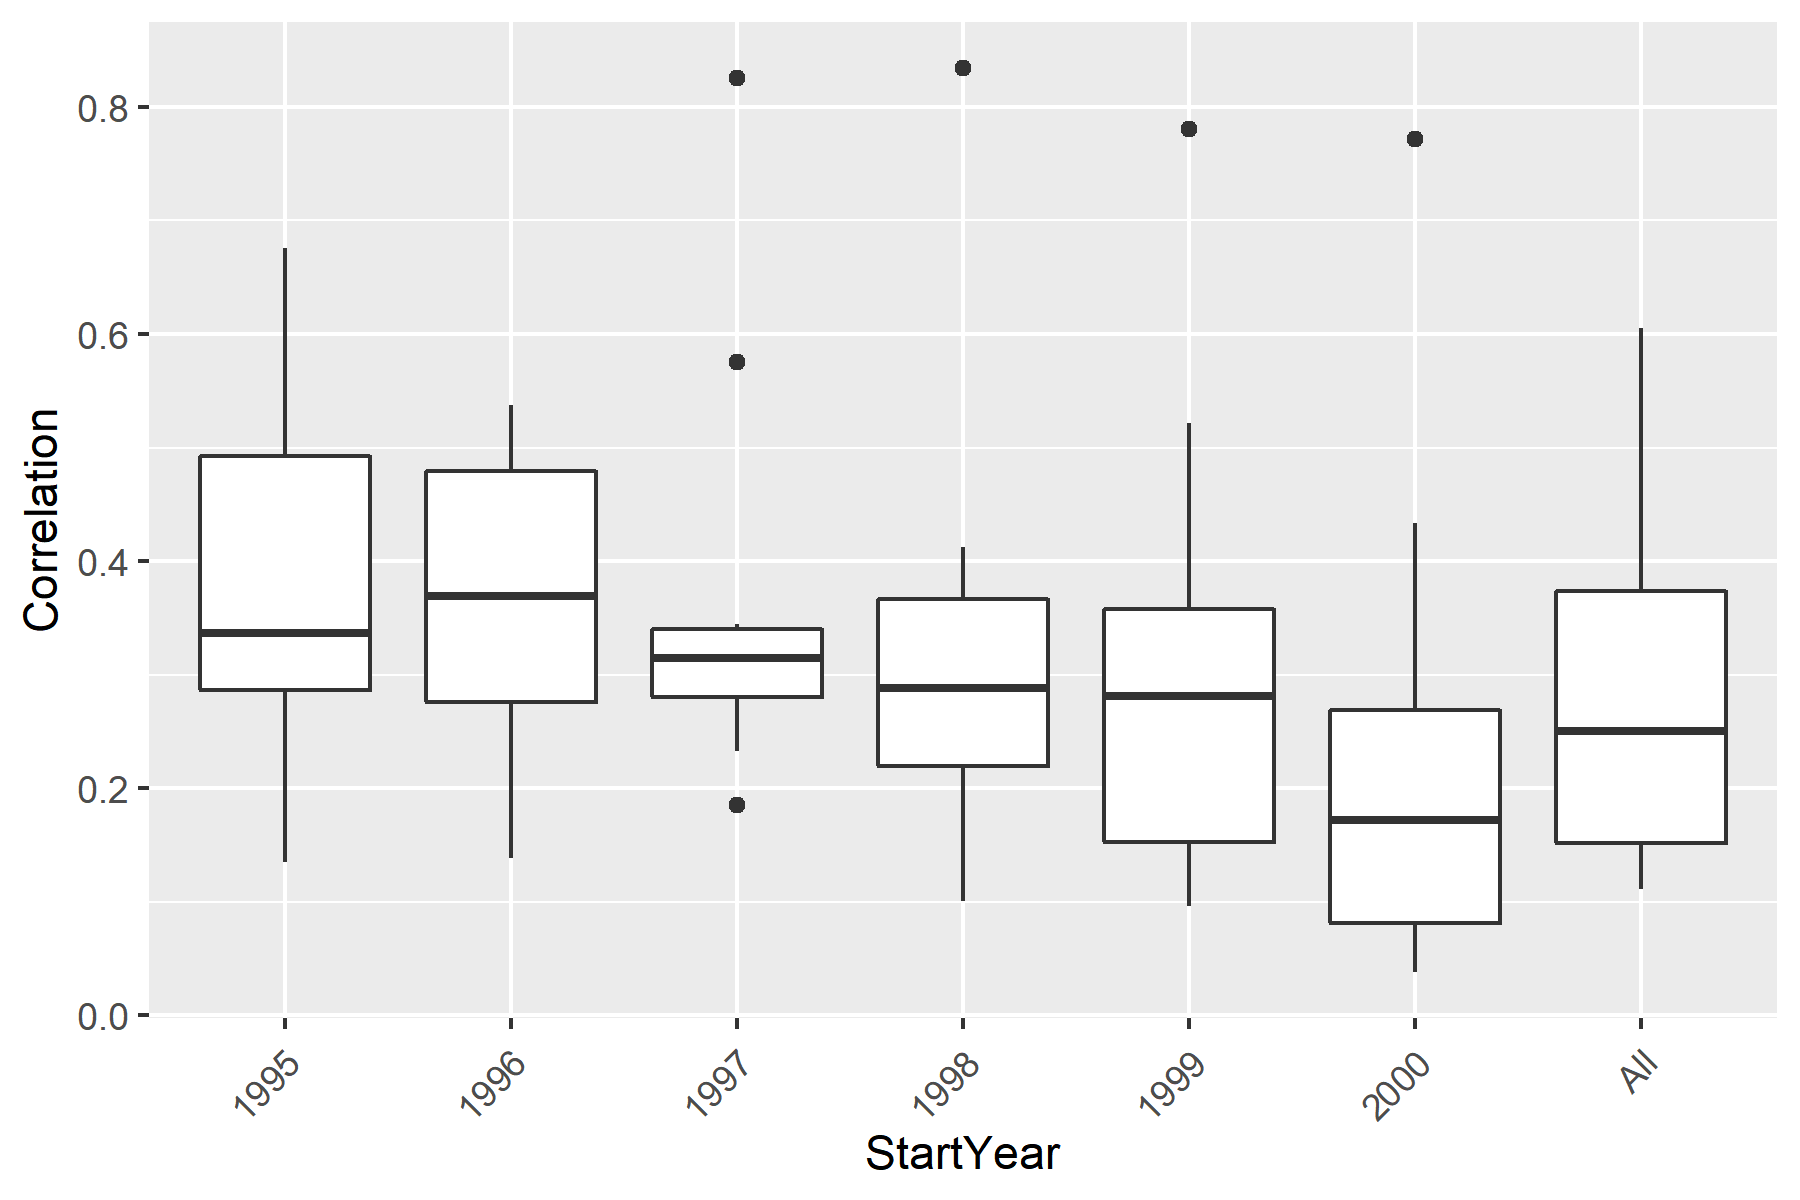
\includegraphics[width=0.6\linewidth]{figure/chinook-RunningCorrelations}}{Figure \ref{fig:chinook-RunningCorrelations}} 

}

\caption{Running correlations in spawner abundances among inlets in 20-year time periods, with the start year of the 20-year period on the X-axis. Each boxplot shows the distribution of pairwise correlations among the 5 inlets (n=10 pairwise correlations).}\label{fig:chinook-RunningCorrelations}
\end{figure}
Within the forward projection model, correlations in spawner abundances among inlets are driven by three model components, each described in more detail below: (1) covariance in exploitation rates among inlets, which is determined from a common interannual exploitation (due to shared exploitation offshore, parameterized from pre-terminal exploitation on Robertson Creek hatchery fish), and additional inlet-specific variability in exploitation due to inlet-specific vulnerability to exploitation, (2) covariance in recruitment residuals among inlets, and (3) covariance in age proportions of recruits among inlets.
\begin{figure}[htb]

{\centering \pdftooltip{\includegraphics[width=0.6\linewidth]{knitr-figs-pdf/chinook-ER-1}}{Figure \ref{fig:chinook-ER}} 

}

\caption{Pre-terminal exploitation rates for Robertson Creek CWT indicator.}\label{fig:chinook-ER}
\end{figure}
\emph{Covariance in exploitation}

We assumed an average exploitation rate as observed for WCVI Chinook in recent years (2010-2019, Robertson Creek indicator, 30\%, Figure~\ref{fig:chinook-ER}, with common interannual variability in exploitation rates due to shared exploitation history offshore.

In forward projections, interannual variability in exploitation rates was assumed to be beta distributed (constrained between 0 and 1), parameterized from estimated pre-terminal exploitation rates for Robertson Creek, with a coefficient of variation (CV) = 0.17 (Table~\ref{tab:chinook-BaseCasePars}). Without data to parameterize inlet-specific variability in exploitation rates, we assumed the inlet-specific variability was half the common (SMU-level) interannual variability (cv=0.085), and varied this in sensitivity analyses from 0 and 0.17 to cover plausible bounds (Figure~\ref{fig:chinook-ERdist}).
\begin{figure}[htb]

{\centering \pdftooltip{\includegraphics[width=0.5\linewidth]{knitr-figs-pdf/chinook-ERdist-1}}{Figure \ref{fig:chinook-ERdist}} 

}

\caption{Variability in projected exploitation rates over time (cv=0.17) and among inlets (cv=0.085), from an average explotation of 0.3.}\label{fig:chinook-ERdist}
\end{figure}
We assumed that inlets were either consistently under- or over-exploited relative to the average over the entire time-series (e.g., due to the spatial and temporal variability in inlet-specific migration patterns affecting vulnerability to fisheries), but that this bias changed over MC trials. Future analyses could include consistent biases in exploitation for specific inlets (e.g., positive biases for southern inlets and negative biases for northern inlets).

In the forward projections, pairwise correlations in projected spawner abundances among inlets were similar to observed pairwise correlations in spawner abundances among inlets (Figure~\ref{fig:chinook-boxplotscvER}). Varying assumptions about variability in exploitation among inlets between cv= 0 and 0.17 did not impact the distribution of correlations in spawner abundances in the projections.
\begin{figure}[htb]

{\centering \pdftooltip{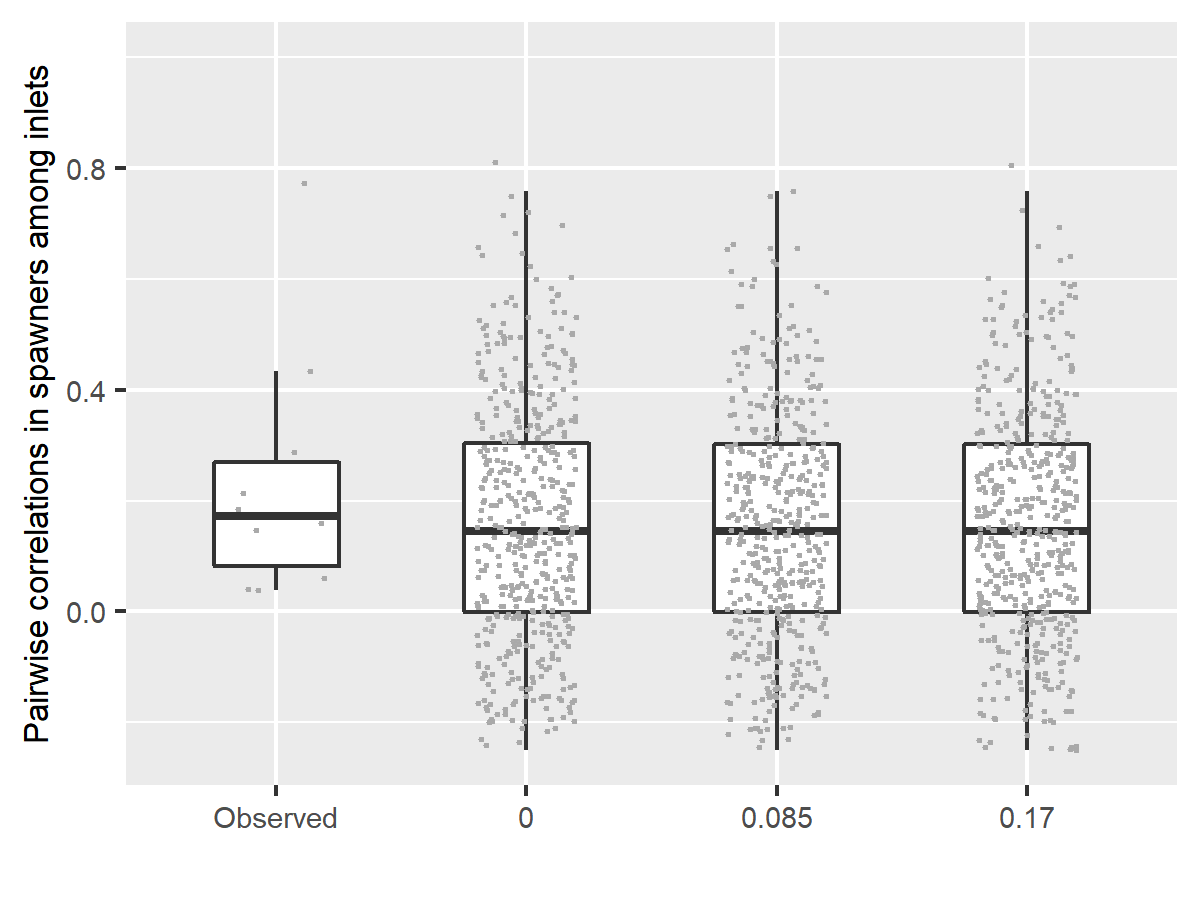
\includegraphics[width=0.6\linewidth]{figure/chinook-compareEscCor-cvER}}{Figure \ref{fig:chinook-boxplotscvER}} 

}

\caption{Distribution of correlations of spawner abundances among inlets for observed data over the most recent 20 years (n=10 pairwise correlations) and projected time-series, with a cv in exploitation rates among inlets = 0, 0.085 or 0.17 (0.17 is equal to the estimated interannual variablity in exploitation rates). }\label{fig:chinook-boxplotscvER}
\end{figure}
\linebreak

\emph{Covariance in recruitment residuals}

We parameterized correlations in recruitment residuals among inlets from the observed correlations in spawner abundances among inlets derived from the WCVI Chinook run reconstruction (D. Dobson and D. McHugh, pers. comm. DFO South Coast Stock Assessment Figure~\ref{fig:chinook-bubbleCor}). In sensitivity analyses, we scaled the pairwise correlations in recruitment residuals among inlets by 0.5 and 0 of the observed spawner correlations (0 representing recruitment residuals that were uncorrelated among inlets in the projections). We then compared the resulting correlations in projected spawner abundances to observed correlations, to ground-truth our assumption and evaluate the extent to which the model provided realistic projections.
\begin{figure}[htb]

{\centering \pdftooltip{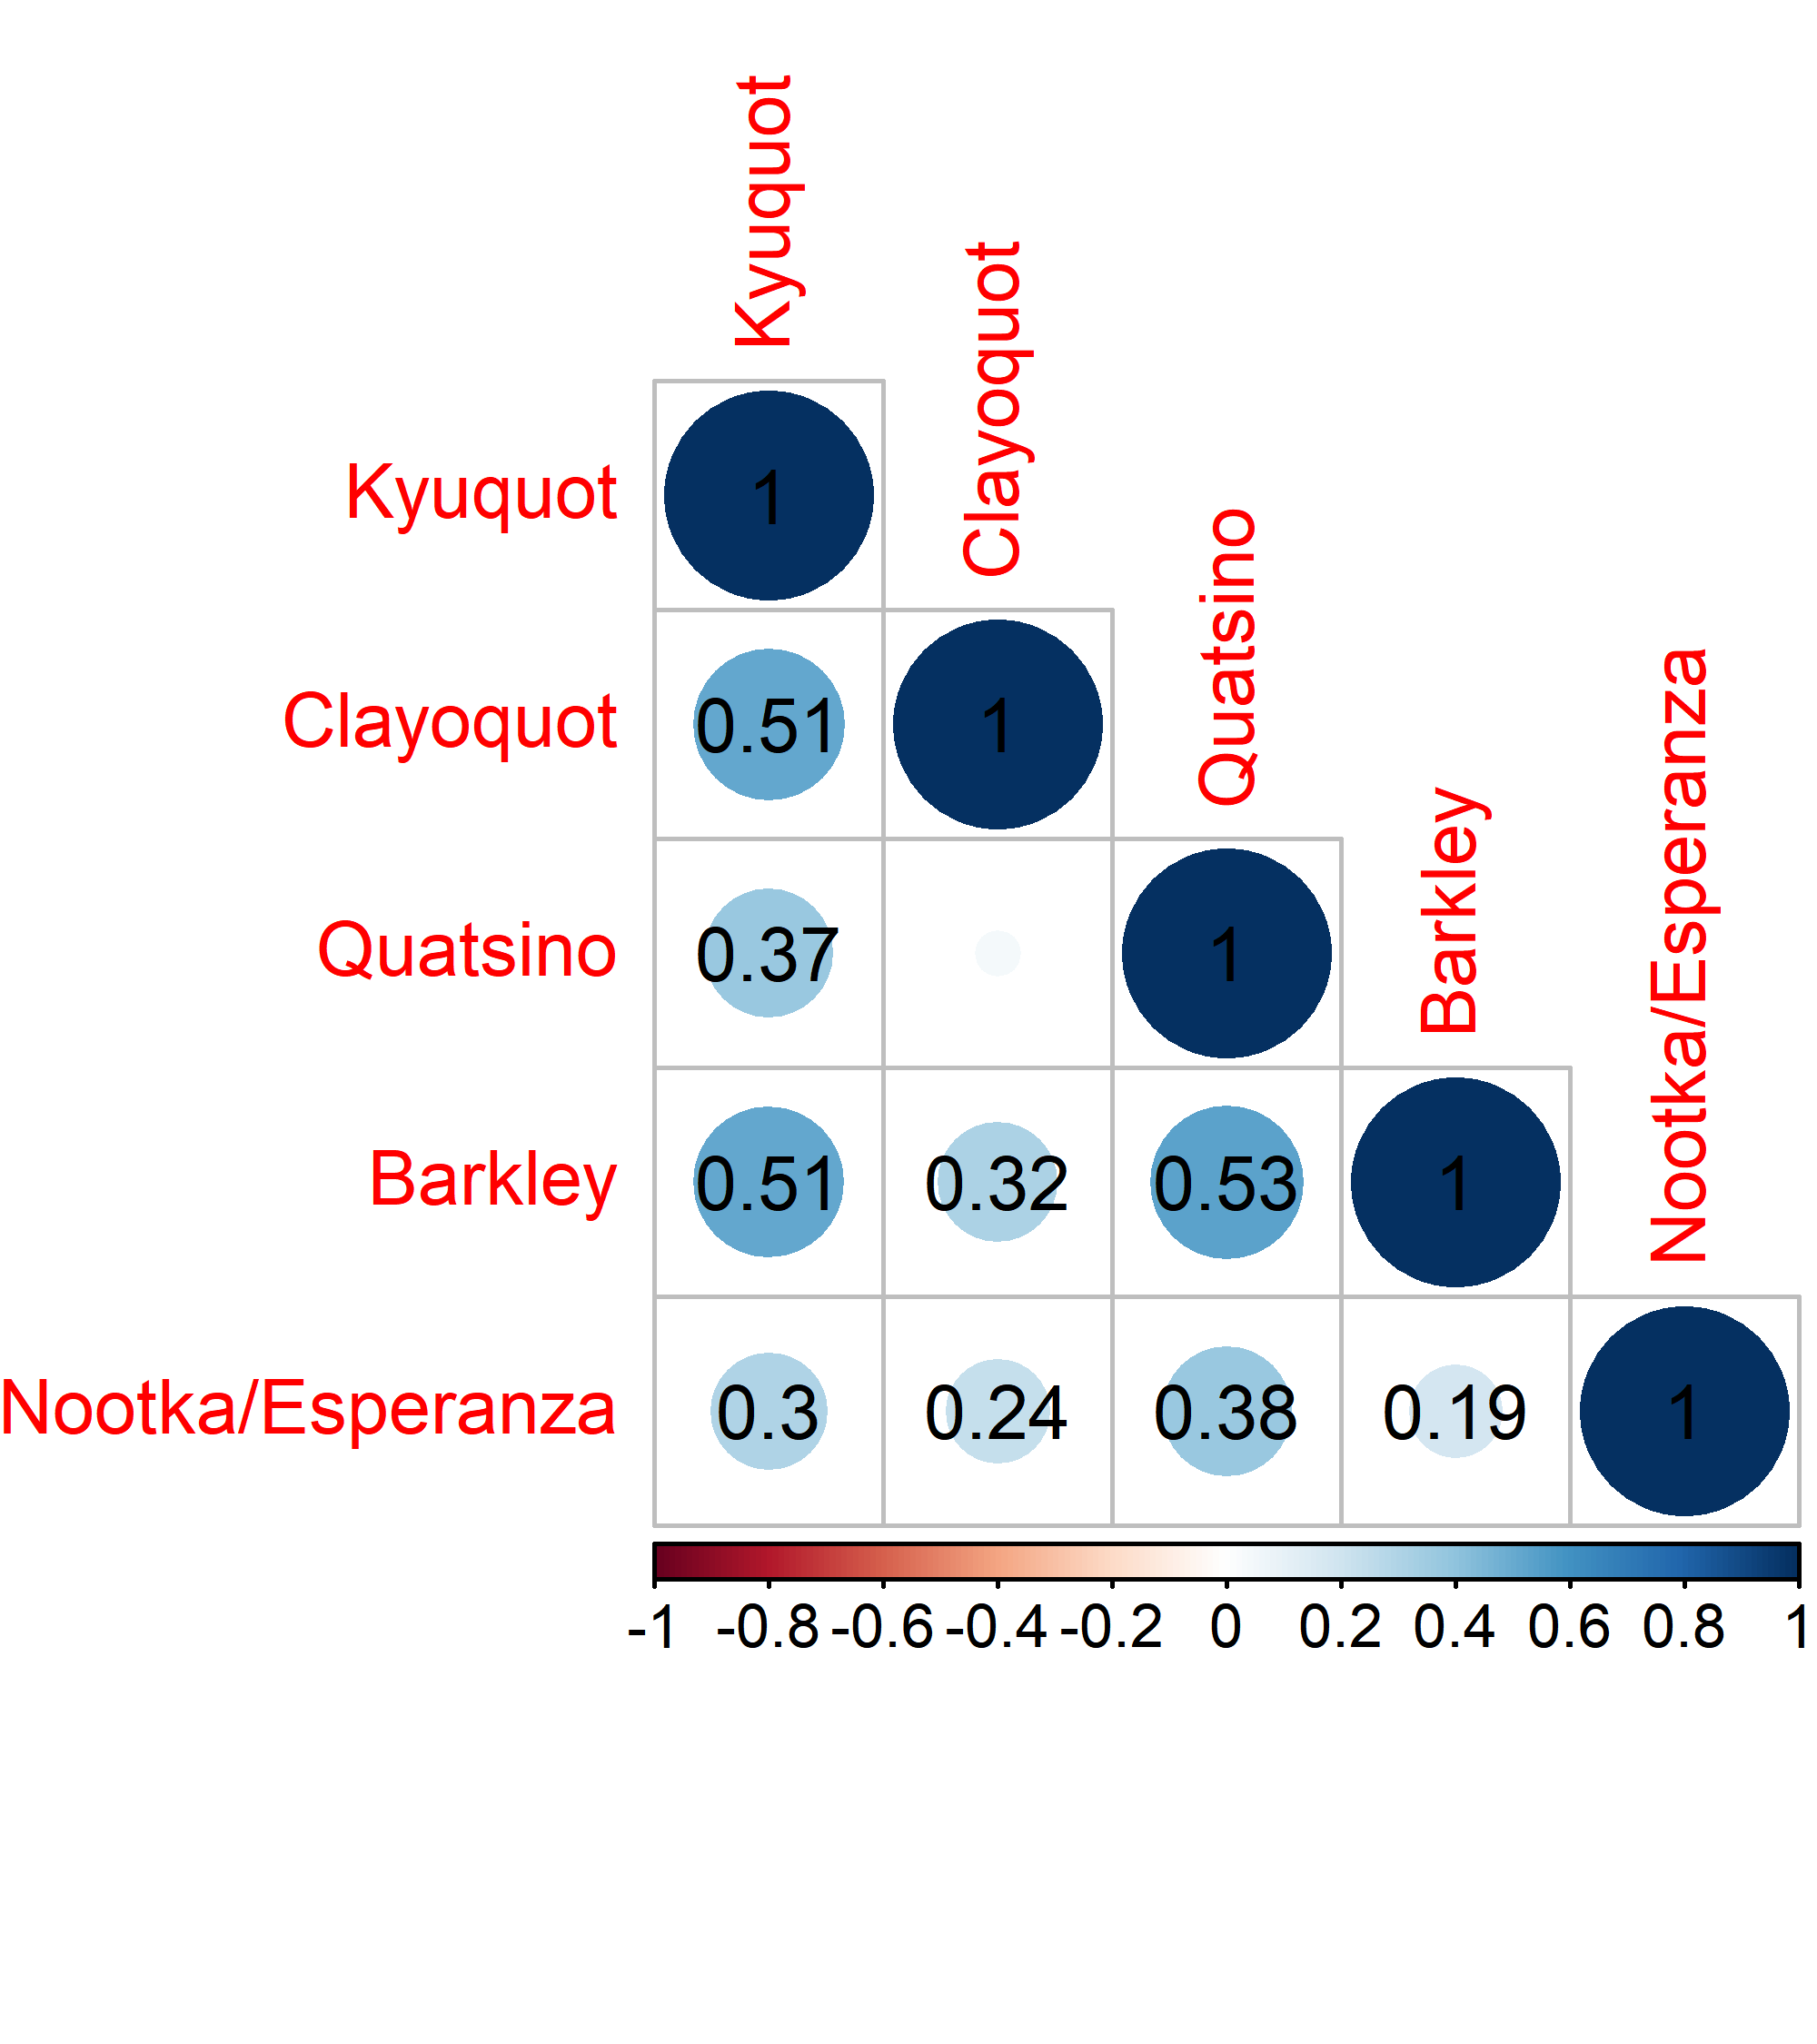
\includegraphics[width=0.4\linewidth]{figure/chinook-SpawnerCorrelation}}{Figure \ref{fig:chinook-bubbleCor}} 

}

\caption{ Bubble plot of correlations in spawner abundances among inlets over time, 1994-2020.}\label{fig:chinook-bubbleCor}
\end{figure}
When we scaled correlations in recruitment residuals to less than observed spawner correlations (i.e., scalar \textless{} 1) the resulting correlations in spawner abundances from the projections were lower than observed correlations (Figure~\ref{fig:chinook-boxplotsRecCorSca}), but were roughly similar when recruitment residuals were scaled to 1. So, for our base case, we assumed correlations in recruitment residuals among inlets were equal to observed correlations among inlets.
\begin{figure}[htb]

{\centering \pdftooltip{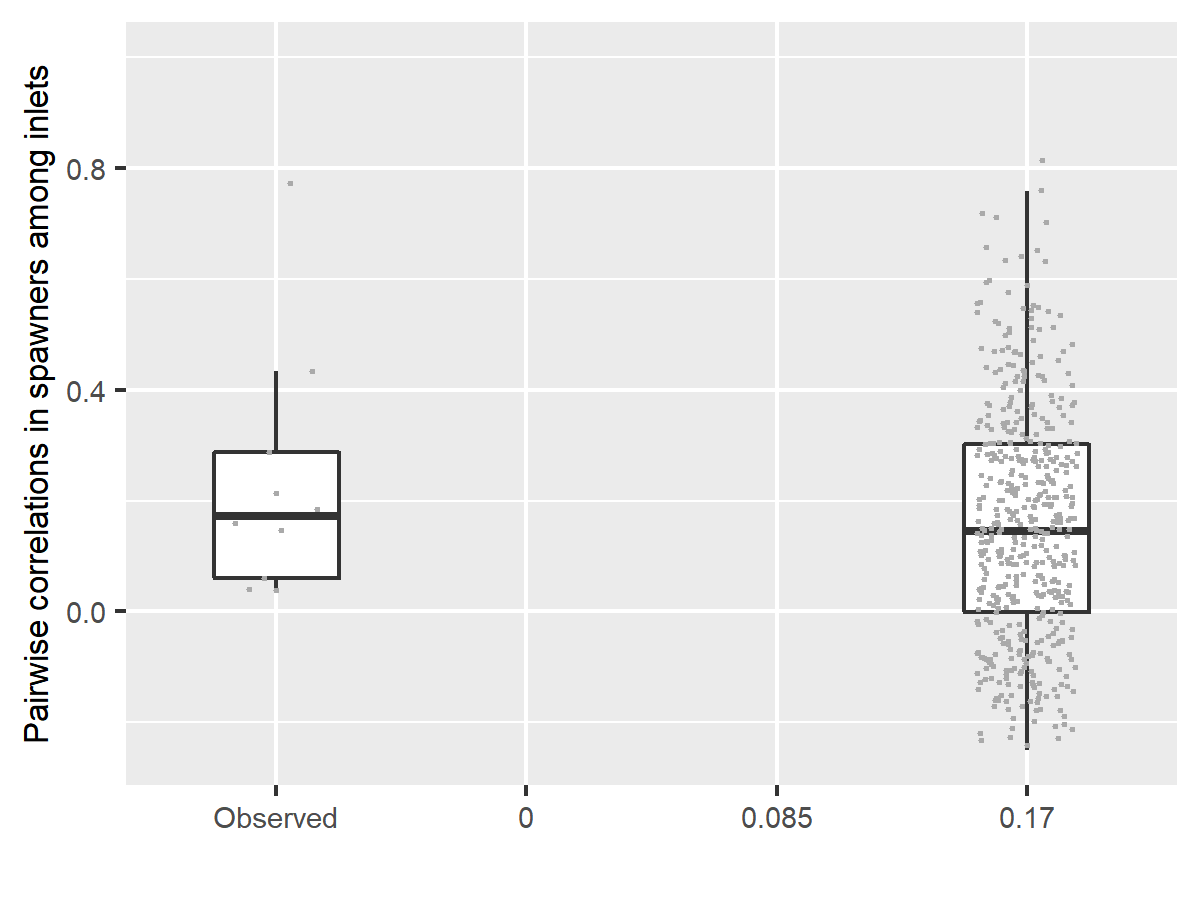
\includegraphics[width=0.5\linewidth]{figure/chinook-compareEscCor-recCorSca}}{Figure \ref{fig:chinook-boxplotsRecCorSca}} 

}

\caption{Distribution of correlations of spawner abundances among inlets for observed data over the most recent 20 years (n=10 pairwise correlations) and projected time-series, assuming a scalar on covariance in recruitment residuals from 1 (equal to observed spawner correlations), 0.5 and 0 (no correlation in recruitment residuals). Projections assume a cv in exploitation rates among inlets = 0.085 (half that of estimated interannual variablity in exploitation rates).}\label{fig:chinook-boxplotsRecCorSca}
\end{figure}
\newline

\emph{Variability in age proportions recruits among inlets}

For the base case, we assumed that age proportions of recruits varied over time and among inlets parameterized from age proportions of recruits calculated for each CU in the WCVI Chinook run reconstruction (D. Dobson pers. comm. DFO Science; inlet-specific age-proportions were not available) (Figure~\ref{fig:chinook-agePpns}). We used the CU-specific mean proportions at each age from the run reconstruction with annual deviations in those proportions based on a multivariate logistic distribution, parameterized from the estimated time-series of age proportions.
\begin{figure}[htb]

{\centering \pdftooltip{\includegraphics[width=0.6\linewidth]{knitr-figs-pdf/chinook-agePpns-1}}{Figure \ref{fig:chinook-agePpns}} 

}

\caption{Time-series of proportions at age in recruitment aligned by brood year, calculated from run reconstruction for West Coast of Vancouver Island Chinook by CU.}\label{fig:chinook-agePpns}
\end{figure}
We ran a sensitivity analysis under an alternative assumption where age proportions varied over years but were constant among CUs. Under this assumption, we found that pairwise correlations of spawner abundances in projections were much higher than those observed (Figure~\ref{fig:chinook-boxplotsAge}), generating time-series that were unrealistic.
\begin{figure}[htb]

{\centering \pdftooltip{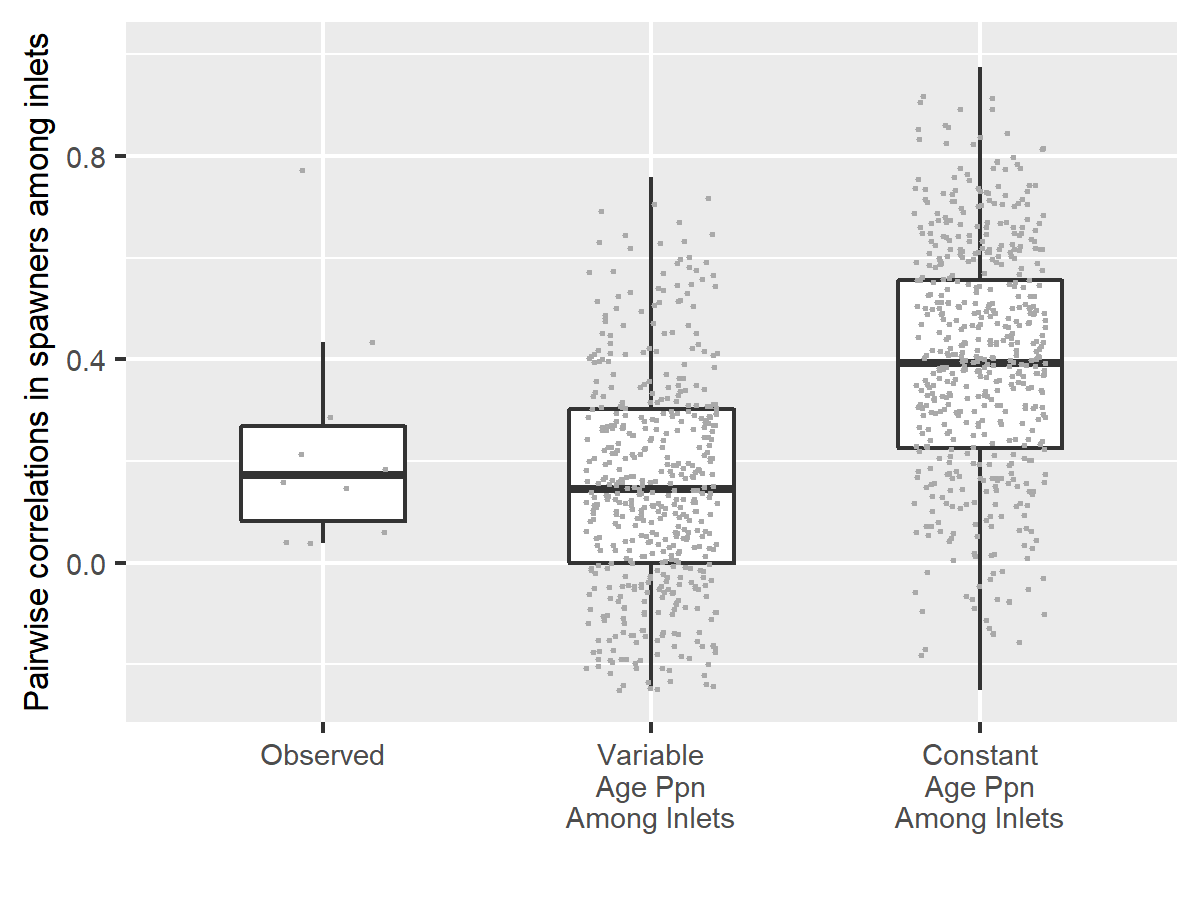
\includegraphics[width=0.6\linewidth]{figure/chinook-compareEscCor-Ages}}{Figure \ref{fig:chinook-boxplotsAge}} 

}

\caption{Distribution of correlations of spawner abundances among inlets for observed data over the most recent 20 years (n=10 pairwise correlations) and projected time-series under the assumptions of variable age proportions among CUs and constant proportions among CUs. We assumed a cv in exploitation rates among inlets = 0.085 (half that of estimated interannual variablity in exploitation rates) in the projections.}\label{fig:chinook-boxplotsAge}
\end{figure}
\hypertarget{results-aggregate-abundance-projection-based-lrps}{%
\subsubsection{RESULTS: AGGREGATE-ABUNDANCE, PROJECTION-BASED LRPS}\label{results-aggregate-abundance-projection-based-lrps}}

Projection-based LRPs were developed under the base-case assumptions of (1) interannual variability in exploitation rates among inlets with a cv = 0.085, (2) correlations in recruitment residuals among inlets equal to observed spawner correlations among inlets, and (3) variability in age proportions among CUs and years. We identified a provisional aggregate abundance LRP with p=0.5 (50\% probability of all inlets being greater than their lower benchmark) equal to 11300 (Figure~\ref{fig:chinook-baseCaseProjLRP}). Provisional LRPs at p=0.66 (``likely'' that all inlets are above their lower benchmarks) is also shown, near 20 000 (Figure~\ref{fig:chinook-baseCaseProjLRP}). Probabilities that all inlets exceeded lower benchmarks did not exceed 0.9 so LRPs at higher p values could not be estimated. Note, the LRP at p=0.66 requires more MC trials for full stabilization and is shown here for demonstration purposes only.
\begin{figure}[!h]

{\centering \pdftooltip{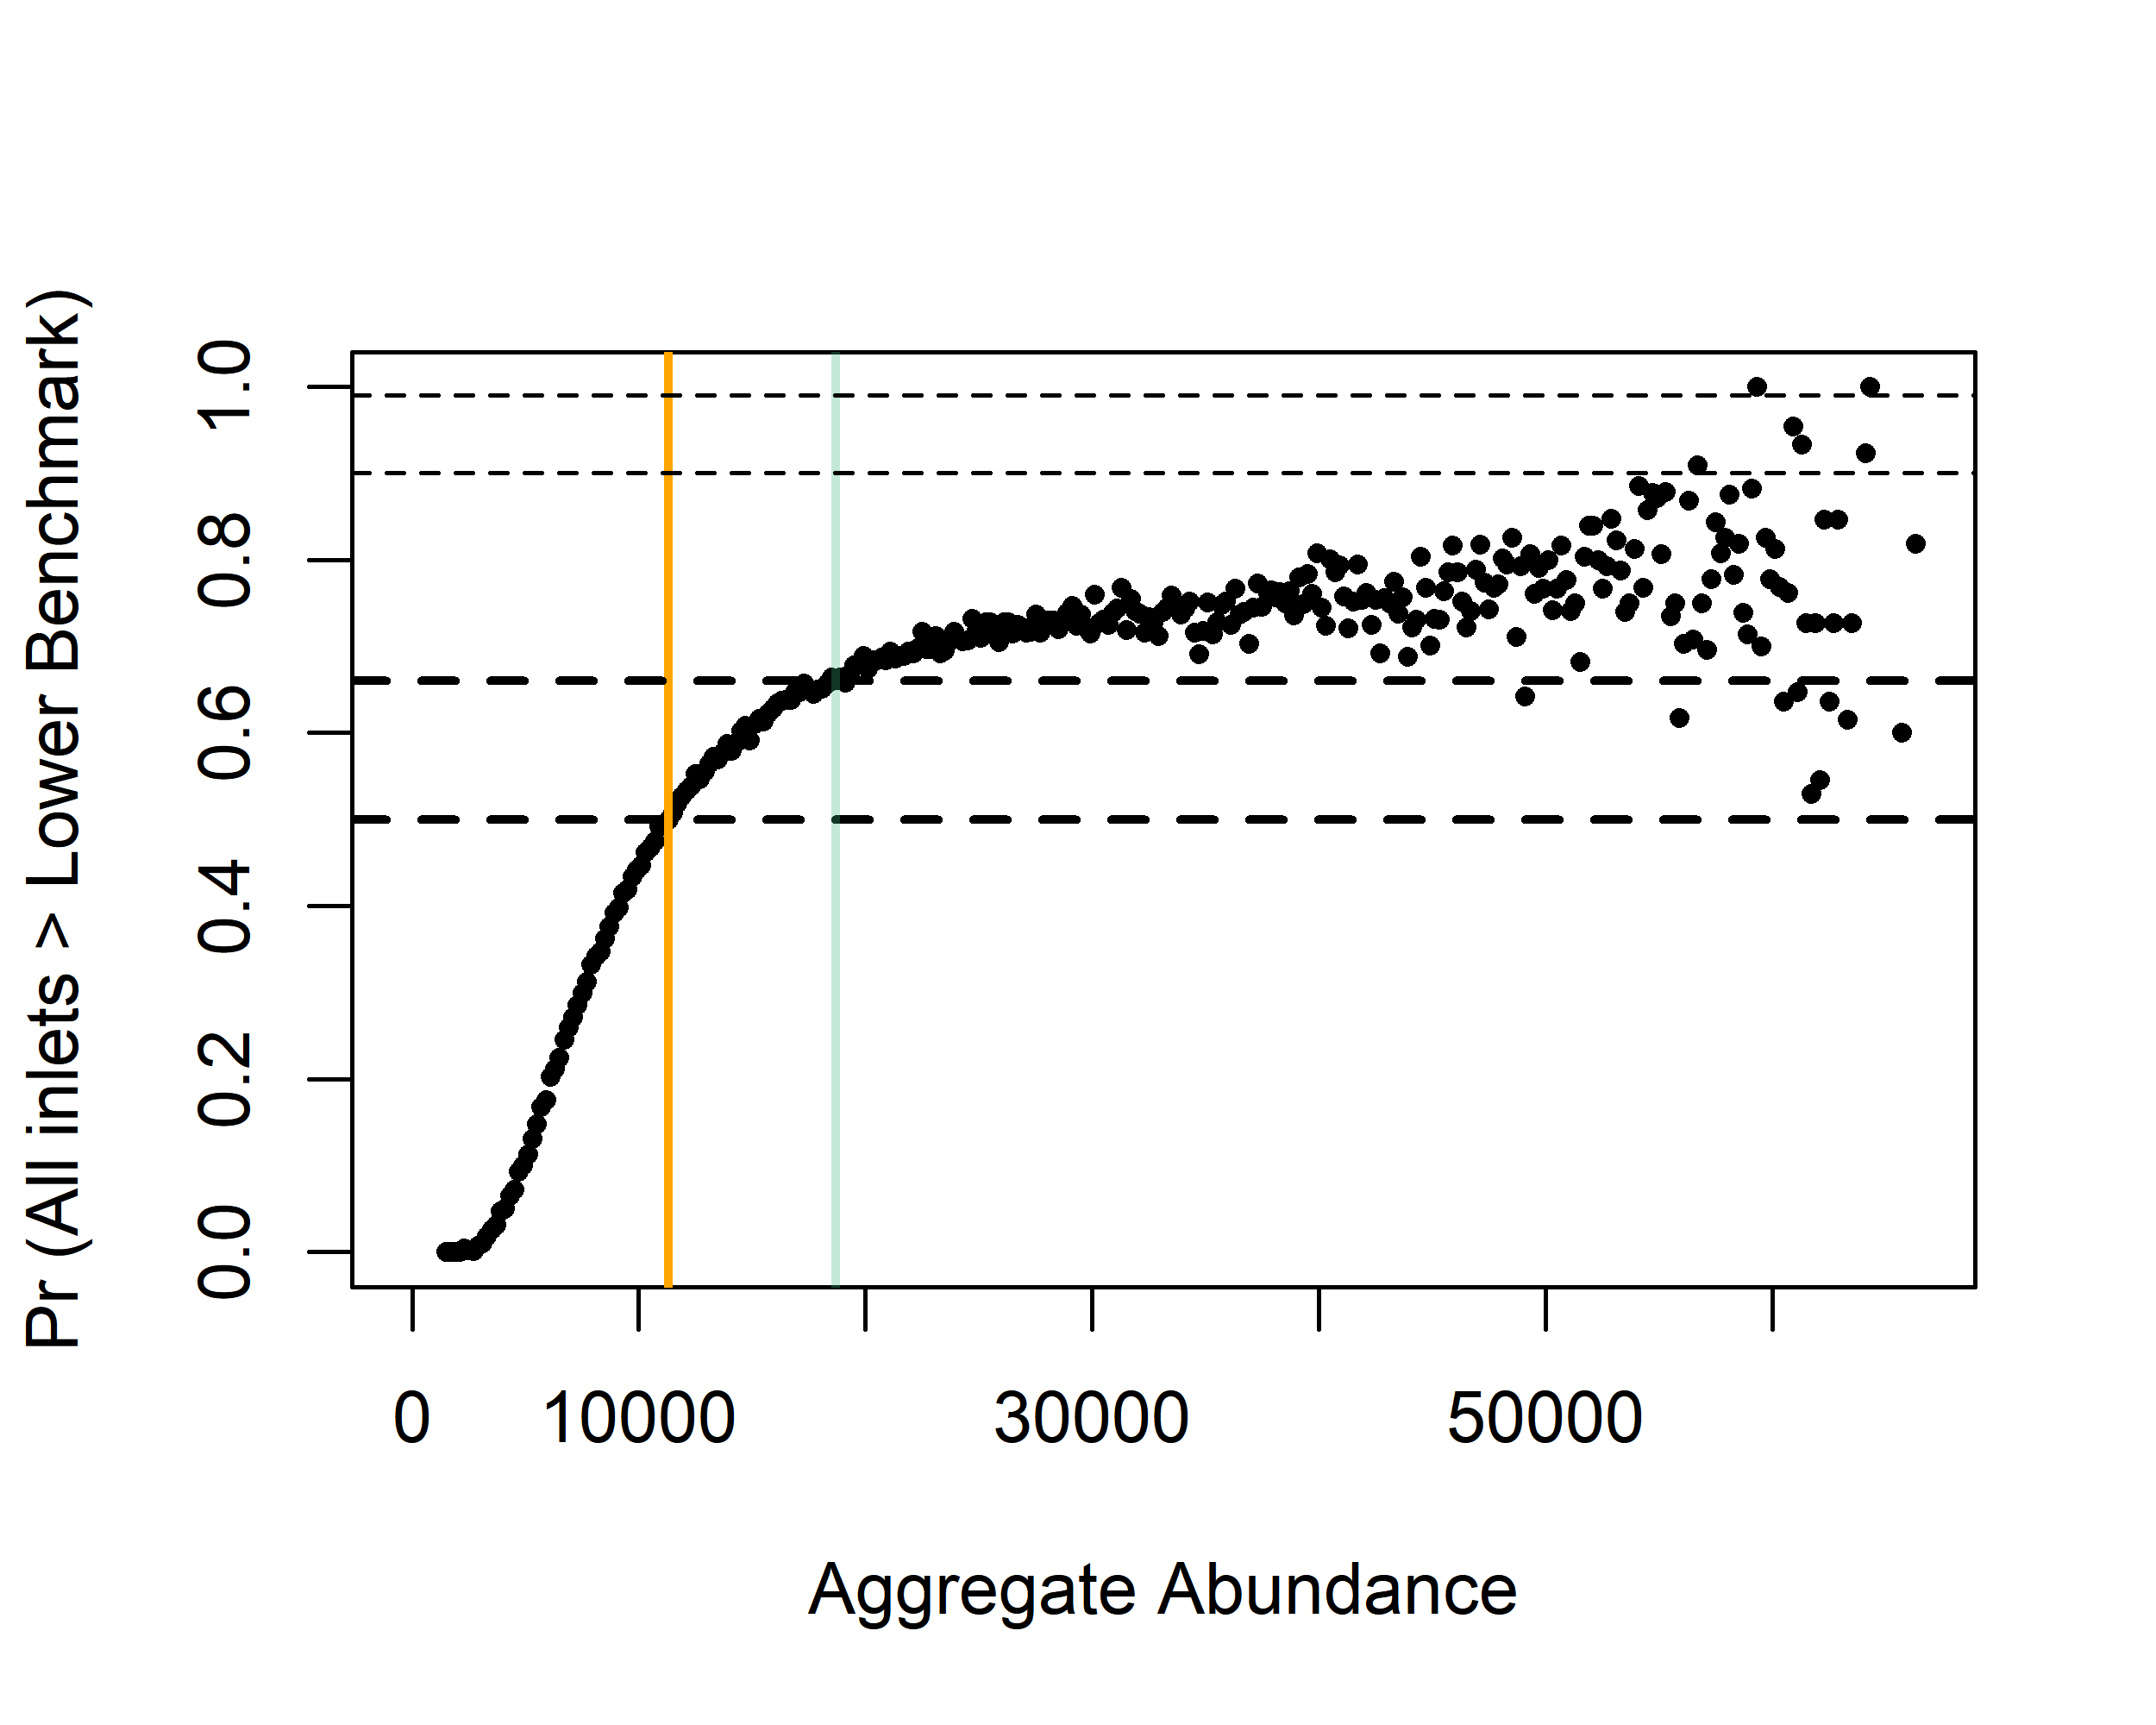
\includegraphics[width=0.6\linewidth]{figure/chinook-baseER-ProjLRPCurve-ALLp}}{Figure \ref{fig:chinook-baseCaseProjLRP}} 

}

\caption{Probability of all inlets being above their lower benchmark along a gradient in aggregate abundances within bins of 200 fish, derived from projections over 30 years and 50,000 MC Trials.  Candidate LRPs at p=0.5 (yellow) and p=0.66 (pale green) are highlighted. Each dot is the proportion of MC trials where all inlets were > lower benchmarks.}\label{fig:chinook-baseCaseProjLRP}
\end{figure}
For the base case parameters, the candidate projection-based LRPs were compared against time-series of aggregate abundances observed for WCVI Chinook salmon (sum of indicator stocks with PNI \textgreater{} 0.5), showing that abundances are currently below these LRPs and have been near or below them over the available time-series (Figure~\ref{fig:chinook-statusProjLRP}).
\begin{figure}[htb]

{\centering \pdftooltip{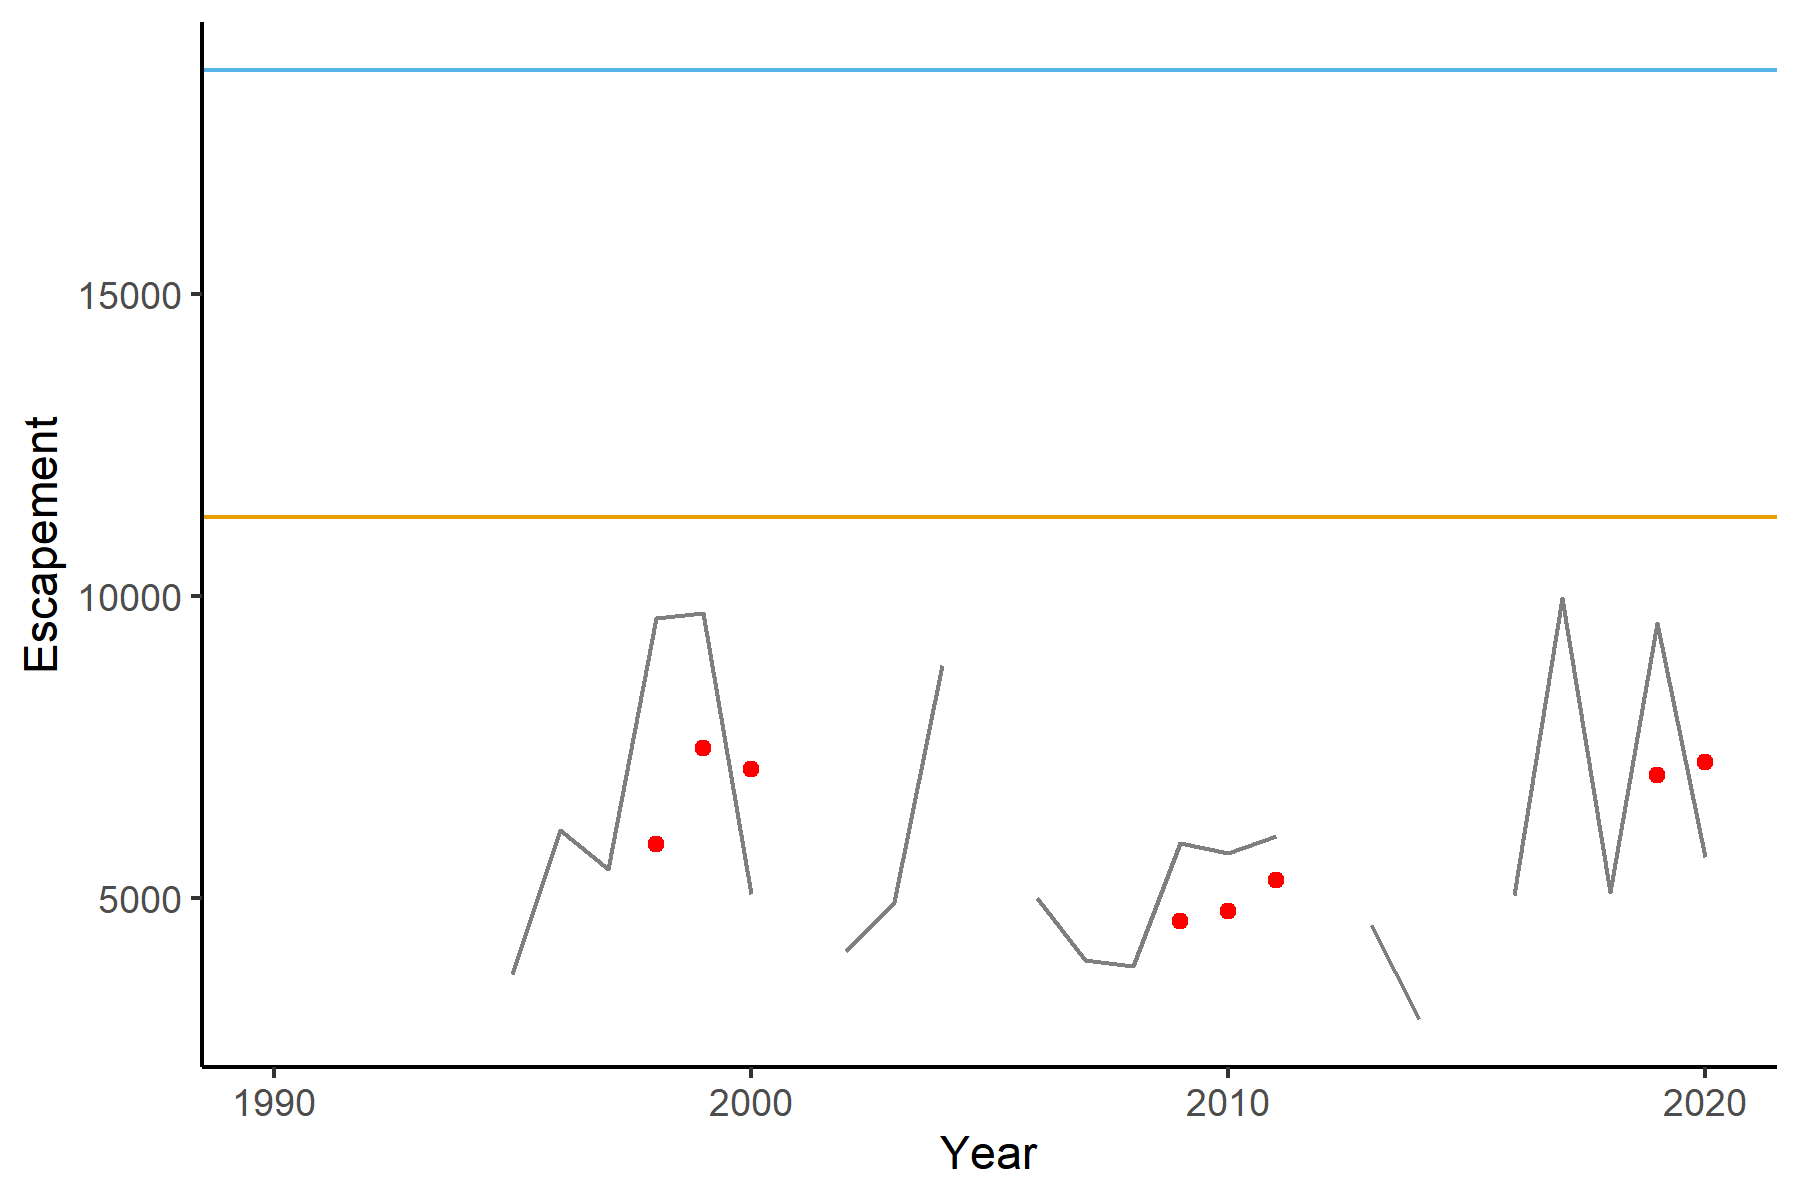
\includegraphics[width=0.6\linewidth]{figure/chinook-SMU-timeseries}}{Figure \ref{fig:chinook-statusProjLRP}} 

}

\caption{Time-series of aggregate escapement for WCVI Chinook (indicator stocks with PNI > 0.5), with projection-based LRPs associated with component inlets being > lower benchmarks at p=0.5 (yellow) and p=0.66 (pale green). Red points are the generational average escapement (geometric mean), red indicating status below LRPs}\label{fig:chinook-statusProjLRP}
\end{figure}
\hypertarget{sensitivity-analyses}{%
\subsubsection{Sensitivity Analyses}\label{sensitivity-analyses}}

We considered sensitivity analyses on interannual variability in exploitation rates among inlets with cv = 0 and 0.17 (Figure~\ref{fig:chinook-projLRPcvER}), and found LRPs at 50\% probability were not sensitive to this assumption.
\begin{figure}[htb]

{\centering \pdftooltip{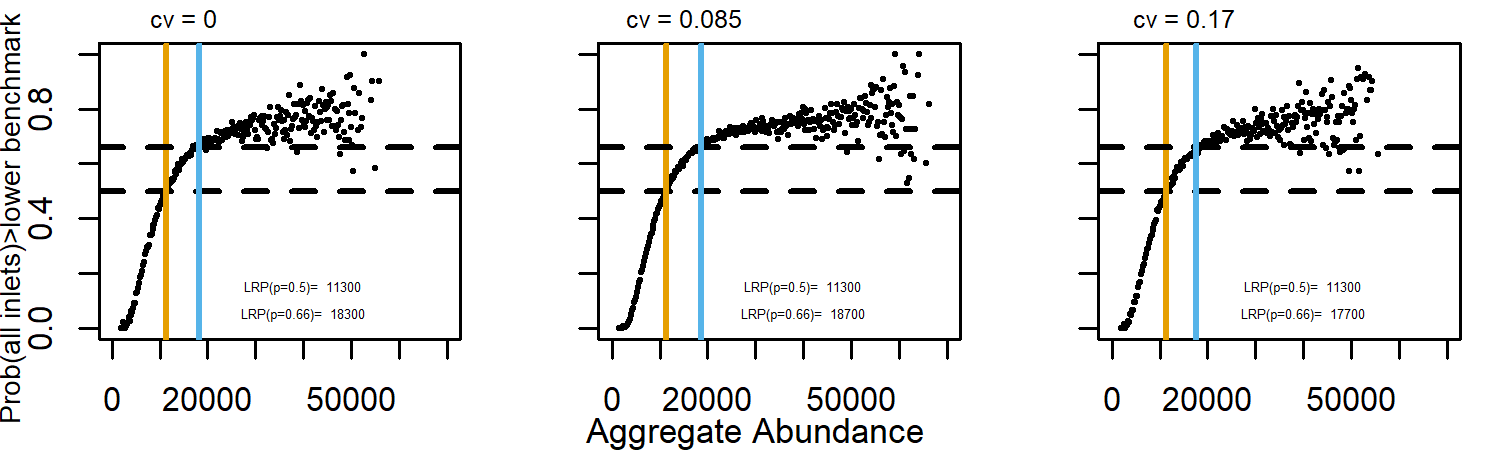
\includegraphics[width=0.6\linewidth]{figure/chinook-cvER-ProjLRPCurve-ALLp}}{Figure \ref{fig:chinook-projLRPcvER}} 

}

\caption{Probability of all inlets being above their lower benchmark along a gradient in aggregate abundances within bins of 200 fish, derived from projections over 30 years and 50,000 MC Trials. The projections assumed variability in ERs among inlets with a cv=0, 0.085, and 0.17.}\label{fig:chinook-projLRPcvER}
\end{figure}
\linebreak

We further considered sensitivity analyses on average exploitation rates from 5-45\% (Figure~\ref{fig:chinook-projLRPER}), where 30\% exploitation was the base case. As exploitation increased, the LRP associated with a specified probability of all inlets being above their lower benchmark also increased. At high exploitation, the depletion of any given inlet was more frequent despite often relatively high aggregate abundances on the remaining inlets.
\begin{figure}[htb]

{\centering \pdftooltip{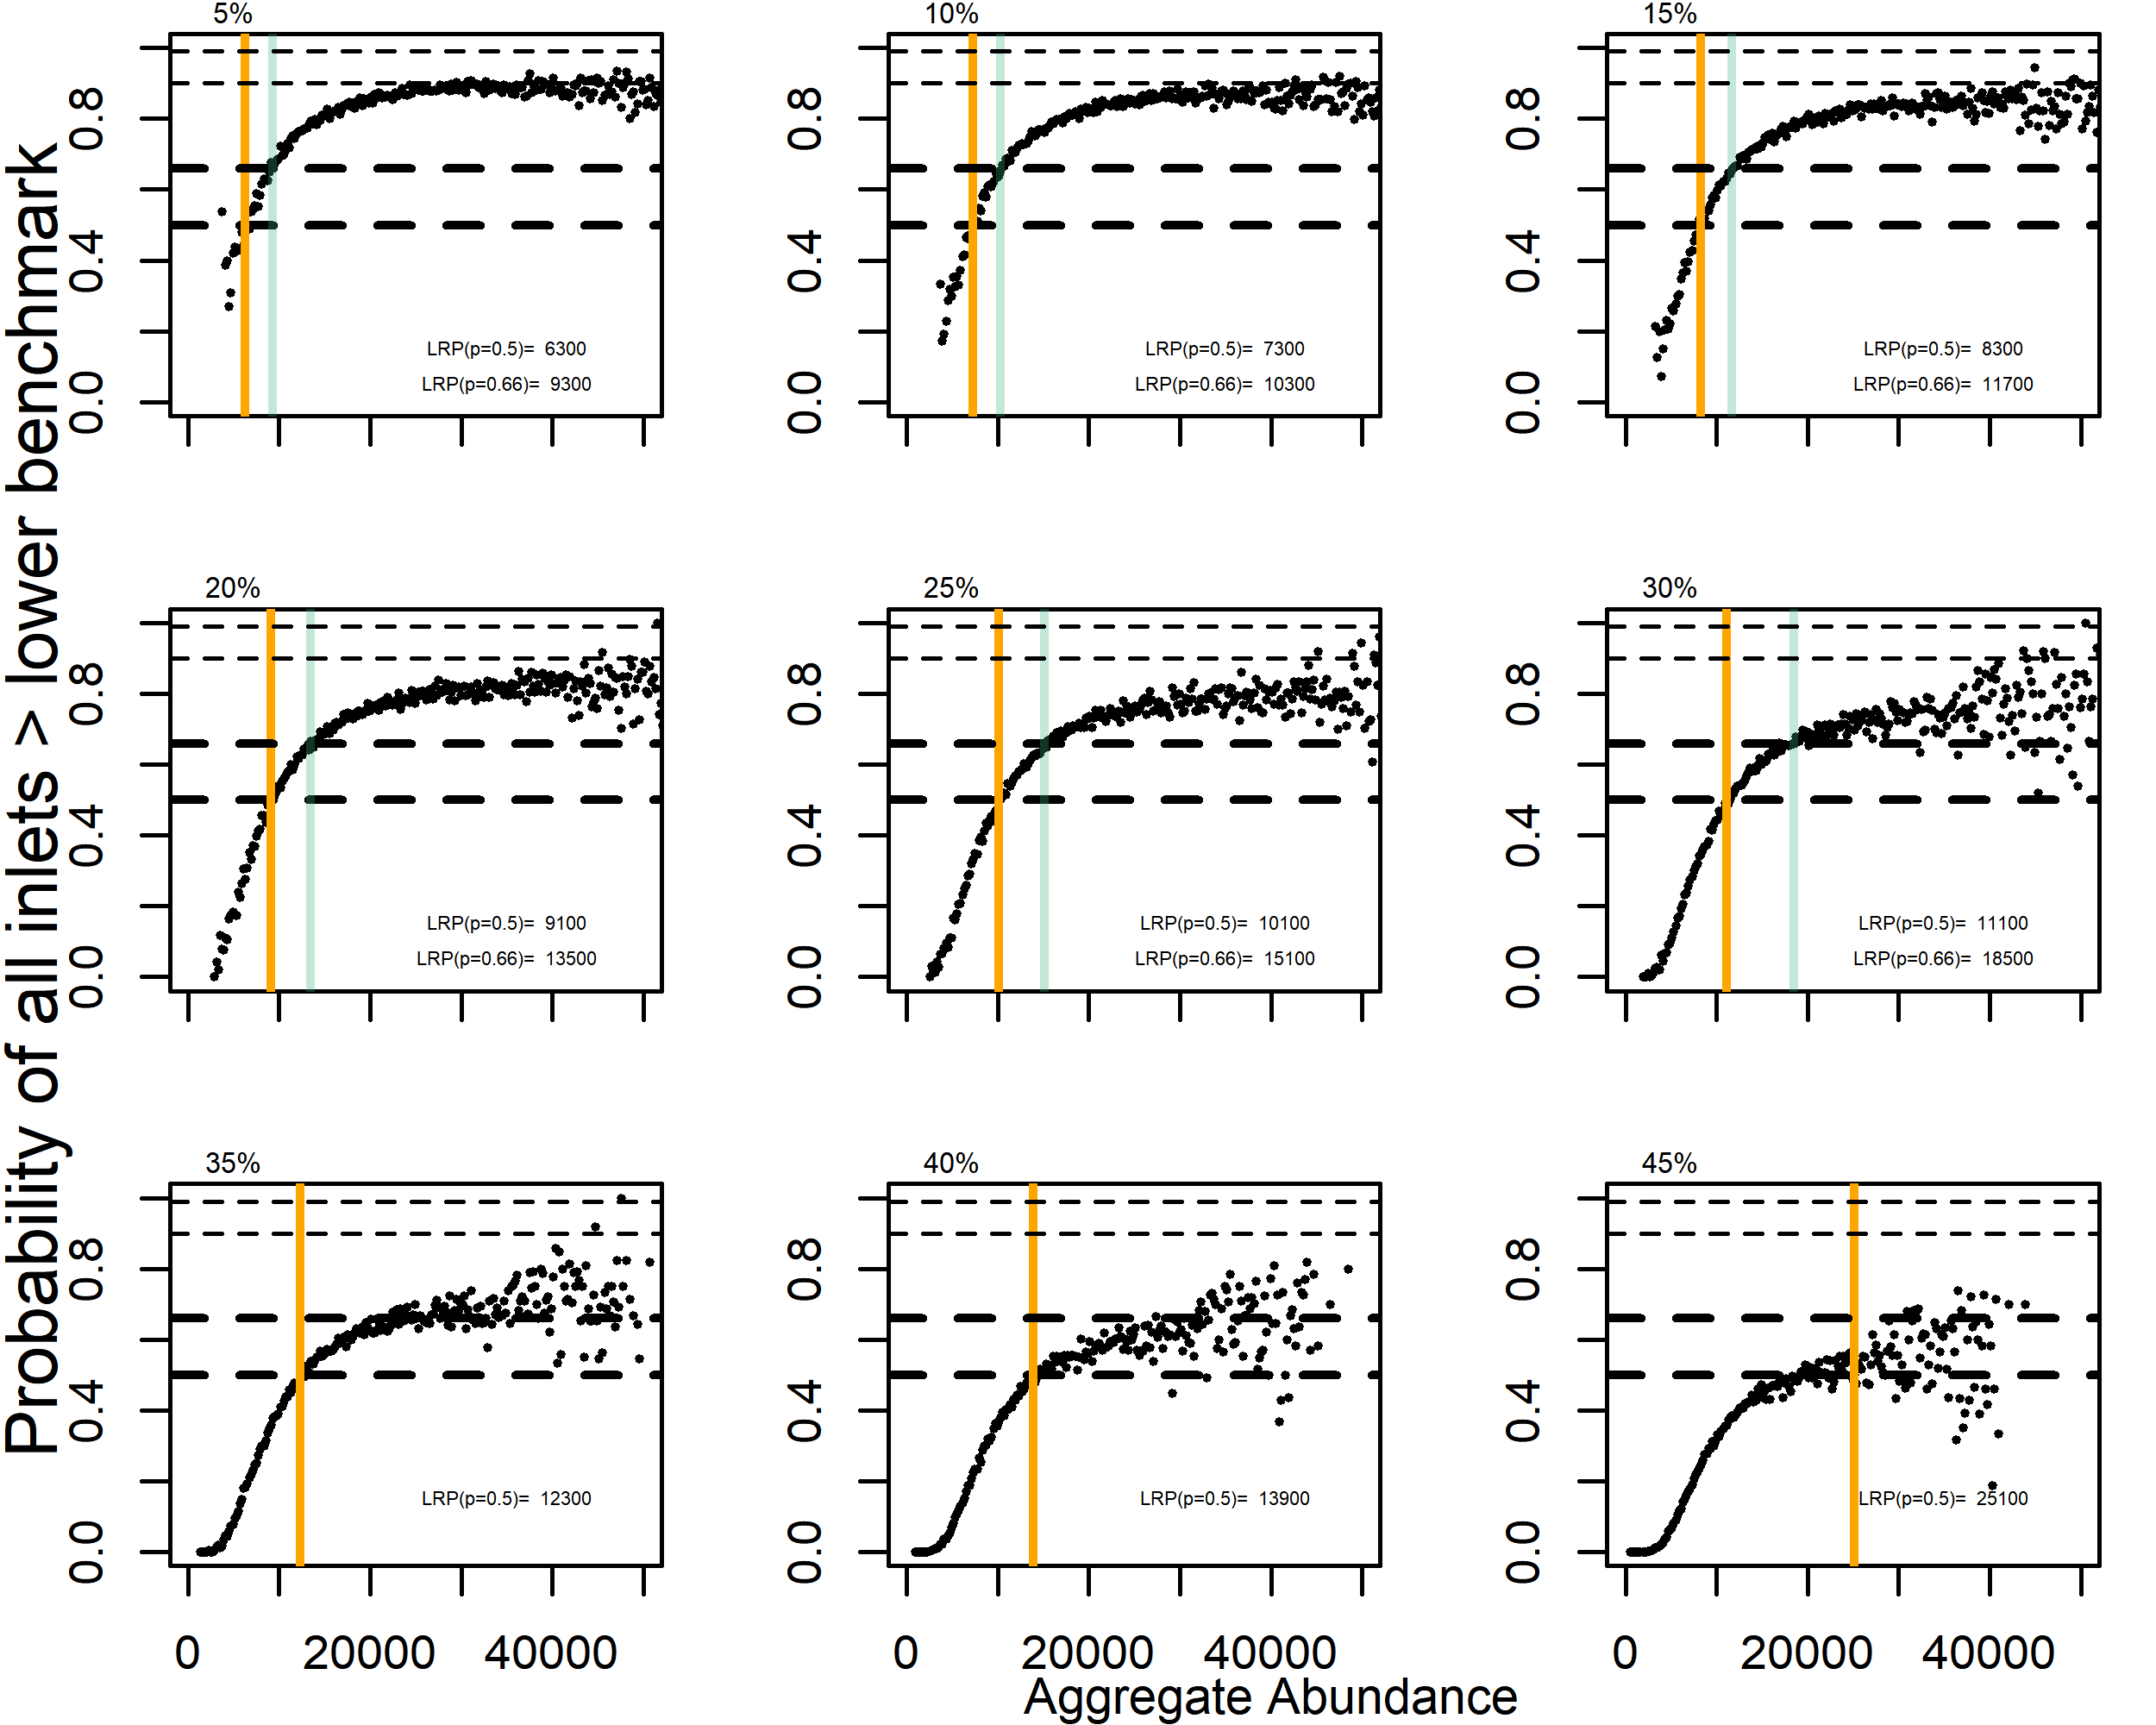
\includegraphics[width=6in]{figure/chinook-ERs-ProjLRPCurve-ALLp}}{Figure \ref{fig:chinook-projLRPER}} 

}

\caption{Probability of all inlets being above their lower benchmark along a gradient in aggregate abundances within bins of 200 fish, derived from projections over 30 years and 50,000 MC Trials, under a range of average exploitation rates from 5-45\%.}\label{fig:chinook-projLRPER}
\end{figure}
\linebreak

Given uncertainty in current and anticipated productivity, projection-based LRPs were evaluated under a range of productivities from 75\% - 150\% of base case estimates. Scenarios with lower productivity (\textless0.75x current estimates) resulted in a large proportion of trajectories with productivity below replacement, for which LRPs could not be estimated.

Projection-based LRPs tended to increase under low productivity and vice versa, a trend that was expected due to the inverse relationship between productivity and inlet-specific \(S_{gen}\) values (\protect\hyperlink{ref-holtCautionsUsingPercentilebased2015}{Holt and Folkes 2015}). At low productivity, \(S_{gen}\) tends to increase, thereby becoming more precautionary. The sensitivity of LRPs to productivity highlights the value of updating benchmarks and projection-based LRPs as productivity changes (Figure~\ref{fig:chinook-projLRPsAlpha}). Our results also show that uncertainty in projections increased under low productivity, likely requiring more random Monte Carlo trials for stabilization at p=0.5.The probability of all inlets being above their lower benchmark rarely met or exceeded 0.66 when productivity was low, so LRPs at this level could not be estimated. When productivity was high, the probability of all inlets being above their lower benchmark rarely dropped below 0.66. At high productivity, LRPs at the p=0.5 level could not be estimated (though estimation may be possible with more Monte Carlo trials). More detailed analyses of LRPs along the entire range of productivities and exploitation was beyond the scope of this case study.
\begin{figure}[htb]

{\centering \pdftooltip{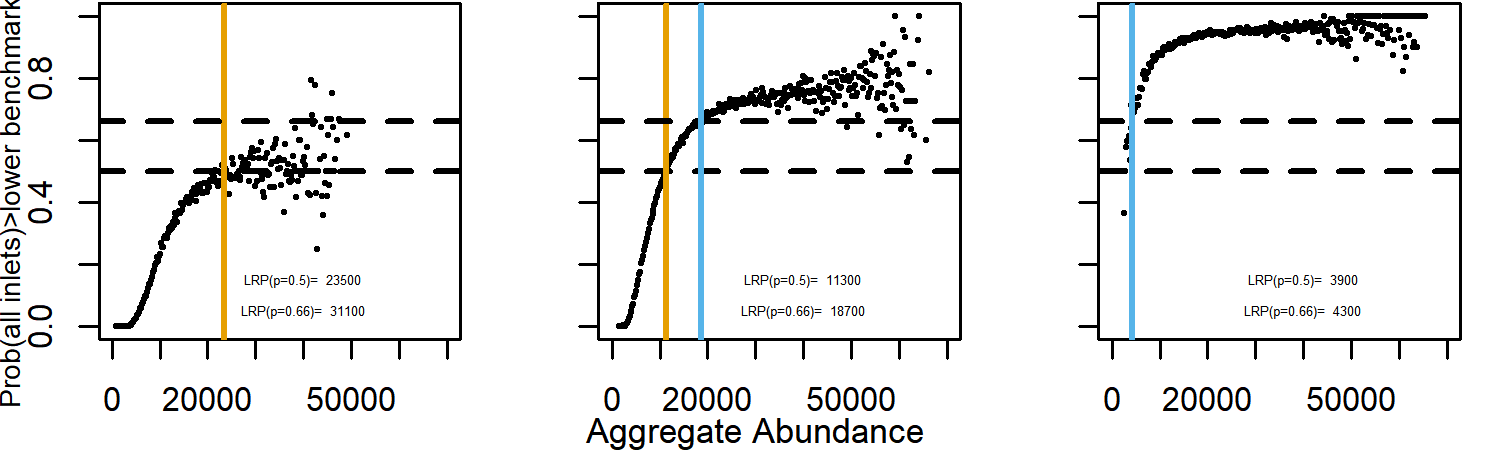
\includegraphics[width=0.8\linewidth]{figure/chinook-Alphas-ProjLRPCurve-ALLp}}{Figure \ref{fig:chinook-projLRPsAlpha}} 

}

\caption{Projection-based LRPs estimated under assumptions of reduced productivity (0.75x of current levels) and increased productivity (1.5x current levels). More MC trials are required for stabilization of LRPs at low productivity.}\label{fig:chinook-projLRPsAlpha}
\end{figure}
\hypertarget{historical-evaluation-of-status-across-lrp-methods-1}{%
\subsection{HISTORICAL EVALUATION OF STATUS ACROSS LRP METHODS}\label{historical-evaluation-of-status-across-lrp-methods-1}}

We evaluated the status of WCVI Chinook using LRPs estimated using the proportion of CUs with all inlets above \(S_{gen}\) and projection-based LRPs, as well as the previously published WSP integrated assessment (status in 2014 only, \protect\hyperlink{ref-dfoIntegratedBiologicalStatus2016}{DFO} (\protect\hyperlink{ref-dfoIntegratedBiologicalStatus2016}{2016})) (Figure~\ref{fig:chinook-retro}). All methods indicate this SMU being below its LRP for years where data are available.
\begin{figure}[htb]

{\centering \pdftooltip{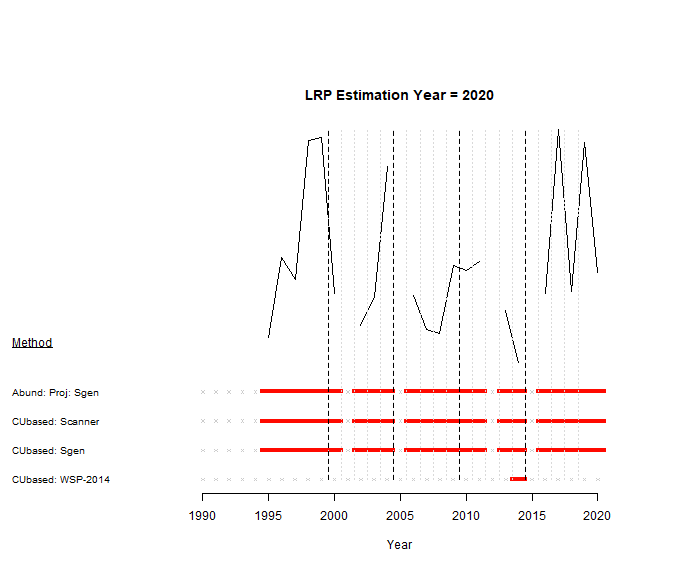
\includegraphics[width=0.8\linewidth]{figure/chinook-statusPlot-withBars2020}}{Figure \ref{fig:chinook-retro}} 

}

\caption{Historical evaluation of status using available methods for estimating LRPs. Red bars indicate status below LRP; grey x's indicate status not available}\label{fig:chinook-retro}
\end{figure}
\hypertarget{overall-conclusions-and-future-analyses}{%
\subsection{OVERALL CONCLUSIONS AND FUTURE ANALYSES}\label{overall-conclusions-and-future-analyses}}

A few key conclusions from this case study are highlighted for broader relevance:
\begin{itemize}
\item
  Status was consistent across the LRP methods that were available, and with a previously published assessment.
\item
  Aggregate-abundance based LRP derived from empirical logistic regression was not possible due to lack of contrast in the time-series.
\item
  Aggregate-abundance based LRPs derived from projections were highly sensitivity to average exploitation. LRPs derived from the base case assumption can not be applied in situations where exploitation has changed, and so cannot be used as a management target \emph{per se}.
\item
  Aggregate-abundance based LRPs derived from projections were also highly sensitivity to underlying population productivities. As productivity declined, LRPs became more precautionary and vice versa.
\item
  Projection-based LRPs at probabilities levels of 90\% and 99\% could not be estimated. Because of the relatively low covariation in dynamics among CUs, the probability of all CUs being above their lower benchmarks were never high, even at high aggregate abundances.
\end{itemize}
In the development of projection-based LRPs, inlets were chosen as the spatial scale of biodiversity required for the sustainability for the SMU. In future analyses, alternative assumptions could be considered, including LRPs derived to maintain diversity at the CU scale by projecting CU-level abundances. Furthermore, future iterations of the multidimensional status assessment approach could include information on the distribution of spawners across sites within CUs or inlets to incorporate additional scales of diversity.

In addition, if projection-based LRPs are considered for this SMU, further work exploring their sensitivity to directional biases in productivity and capacity is warranted.

\hypertarget{ISCchumChapter}{%
\section{CASE STUDY 3: INSIDE SOUTH COAST CHUM - NON-FRASER}\label{ISCchumChapter}}

\hypertarget{context-2}{%
\subsection{CONTEXT}\label{context-2}}

The `Inside South Coast Chum - Non-Fraser' (ISC-NF Chum) SMU includes seven CUs of Chum Salmon from rivers that drain into Johnstone Strait and the Salish Sea along the mainland of British Columbia and the east coast of Vancouver Island (Figure~\ref{fig:chum-map}; \protect\hyperlink{ref-holtbyConservationUnitsPacific2007}{Holtby and Ciruna} (\protect\hyperlink{ref-holtbyConservationUnitsPacific2007}{2007})). This area includes deep fjords, glaciers, large rivers, and small coastal streams. Chum salmon CUs spawning in the Fraser River watershed are not included in this SMU. They have been categorized as a separate `Inside South Coast Chum - Fraser' SMU. While these two SMUs have substantial overlap in ocean fisheries, they have been separated into two SMUs based on differences in terminal fishery impacts and freshwater habitats.
\begin{longtable}[]{@{}lcccc@{}}
\caption{\label{tab:CU-summary}The seven Conservation Units in the Inside South Coast Chum Non-Fraser Stock Management Unit. Note that only fall run streams were used in this study due to run reconstruction methods. LBM = Lower Benchmark, UBM = Upper Benchmark used for percentile benchmarks.}\tabularnewline
\toprule
CU Name & Fall run streams & Summer run streams & LBM & UBM \\
\midrule
\endfirsthead
\toprule
CU Name & Fall run streams & Summer run streams & LBM & UBM \\
\midrule
\endhead
Southern Coastal Streams & 23 & 8 & NA & NA \\
North East Vancouver Island & 17 & 0 & 50\% & 50\% \\
Upper Knight & 3 & 2 & 50\% & 50\% \\
Loughborough & 37 & 0 & 50\% & 50\% \\
Bute Inlet & 4 & 1 & NA & NA \\
Georgia Strait & 125 & 1 & 25\% & 50\% \\
Howe Sound-Burrard Inlet & 66 & 0 & 25\% & 50\% \\
\bottomrule
\end{longtable}
The ISC Chum SMU is considered data-limited. While escapement series are available for many streams starting in 1953, several series are incomplete and require infilling assumptions (i.e., not all streams counted each year, some CUs have no counts in some years). In addition, run reconstructions of recruitment are uncertain, making the development of benchmarks based on spawner and recruitment data problematic. There are also no data on marine survival (although there are some scale/growth data in \protect\hyperlink{ref-debertinMarineGrowthPatterns2017}{Debertin et al.} (\protect\hyperlink{ref-debertinMarineGrowthPatterns2017}{2017})). Other unique characteristics of this SMU include high contrast in abundance among CUs and relatively low correlation in abundance among CUs over time. The SMU covers a large area with many diverse watersheds, flow regimes, and ocean entry locations. Wild Salmon Policy status assessments have not been done on any ISC Chum CUs. (\protect\hyperlink{ref-godboutStockStatusWild2004}{\textbf{godboutStockStatusWild2004?}}) identified variable but stable status in the central and southern portion of the SMU, with declines in the north, especially in the region defined by Southern Coastal Streams CU. (\protect\hyperlink{ref-holtEvaluatingBenchmarksBiological2018}{\textbf{holtEvaluatingBenchmarksBiological2018?}}) found similar results in a provisional assessment of status. At this time, a peer-reviewed integrated status assessment has not been developed for ISC chum. \emph{\textcolor{cyan}{LW: Does @godboutStockStatusWild2004 not count as a full status assessment?}}.

Step 3 of the Guidelines for Applying LRPs gives guidance on what evidence would be required to use known status of some CUs for other CUs that are data-limited. This is relevant for the ISC Chum case study because two CUs have no observations in some years (Upper Knight and Bute Inlet). For data deficient CUs to be represented by CUs with data, there needs to be evidence that the data deficient CUs have similar threats, environmental drivers, biological characteristics, and habitat capacity (Guidelines paper, Section 4.1.3).

Upper Knight and Bute Inlet CUs are both associated with long fjords that run from the Broughton Archipelago through the Coast Mountains. They include rivers with headwaters in the Cariboo region farther inland than other CUs in the SMU (Fig.~\ref{fig:chum-map}). Southern Coastal Streams, Georgia Strait, and Howe Sound-Burrard Inlet also include portions of the Coast Mountains and some glaciers, but to a lesser extent and their inlets are shorter and their watersheds do not go as far inland. Upper Knight and Bute Inlet are unique in that they are the only CUs in the SMU that only include watersheds that drain into the upper end of long inlets. They are both more remote than the other CUs, which is part of why there are fewer observations \emph{\textcolor{cyan}{LW: check with PVW if this is true}}.

Chum from these CUs are exposed to different threats to habitat, survival and productivity than the other five CUs. While these CUs have, on average, lower impacts from forest harvest, impervious area, and roads, they have larger impacts from forest defoliation and pests (pacificsalmonfoundationPacificSalmonExplorer2021). They may also have different levels of risk from disturbances such as glacier melt, avalanches, debris flows, and floods because they have large melting glaciers associated with lakes, steep slopes, and unstable terrain. The glacial lake outburst flood that caused a debris flow in the Southgate River in November 2020 is one example of such a an event. These events are capable of killing an entire brood year of eggs/alevins and reshaping habitat with impacts on spawning habitat and stream ecosystems for many years. They can also change water quality in marine habitats. These catastrophic events may be less likely in watersheds with gentler topography and that lack glaciers and glacial lakes. The hydrology of these two CUs likely differs from that of other CUs with more low-lying topography. These watersheds have large glaciers and high amounts of snowmelt, compared to more low-elevation coastal watersheds with more rain-dominant hydrographs. Marine conditions when smolts enter the ocean in these systems may vary from that of the other five CUs, as they are entering the upper ends of large fjords. Regarding biological characteristics, Bute Inlet and Upper Knight have a higher proportion of summer-run populations of chum (\ref{tab:CU-summary}). Productivity (recruits per spawner) of the Upper Knight and Bute Inlet CUs (using CU-level infilling, which introduces error) have the largest magnitude of variability in the SMU, with very productive years (\textgreater100 recruits per spawner) and low productivity years, and boom and bust cycles of abundance. These CUs also have lower habitat capacity, with fewer streams with chum spawners than the other CUs (\ref{tab:CU-summary})\emph{\textcolor{cyan}{LW: check with PVW if this is just fewer monitored streams}}. Based on these difference, the burden of proof is not met, and we cannot infer the status for Bute Inlet and Upper Knight from the other CUs. Note that these criteria used to evaluate whether status can be borrowed for these CUs extends to whether reliable spawner escapement data can be infilled using escapement in the other CUs. Thus, these CUs are dropped for years with no spawner data in this case study. In other SMUs where the quality of data differs for a subset of CUs, careful consideration should be given to whether abundance, productivity, and their trends can be reliably estimated using data from CUs with data of higher quality.

Benchmarks based on spawner-recruit relationships are unreliable if there is uncertainty in the spawner and recruit data. One alternative is benchmarks calculated as a percentile of the historical CU-level spawner abundance time series (percentile benchmarks). Previous work on developing WSP benchmarks for Inner South Coast Chum has shown that percentile benchmarks can be comparable to those based on stock-recruit relationships when productivity is relatively high and harvest is relatively low ((\protect\hyperlink{ref-holtEvaluatingBenchmarksBiological2018}{\textbf{holtEvaluatingBenchmarksBiological2018?}})). In other cases, percentile benchmarks may be inappropriate due to low productivity, high harvest, and because they do not account for non-stationarity in recruitment dynamics ((\protect\hyperlink{ref-holtEvaluatingBenchmarksBiological2018}{\textbf{holtEvaluatingBenchmarksBiological2018?}})).

We chose the ISC-NF Chum SMU as a case study because we were interested in exploring LRP options for a data-limited SMU. We applied LRPs based on two methods: proportions of CUs above their lower benchmark, and logistic regression based on aggregate abundance. For proportions, we used percentile benchmarks and multi-dimensional status assessment to determine the status of component CUs. For the logistic regressions, we used percentile and \(S_{gen}\) benchmarks. However, after attempting \(S_{gen}\) benchmarks we decided not to use them because of unreliable stock-recruit data. Using recruitment data would not satisfy reliability principles in Holt et al.~(in review).
\begin{figure}[htb]

{\centering \pdftooltip{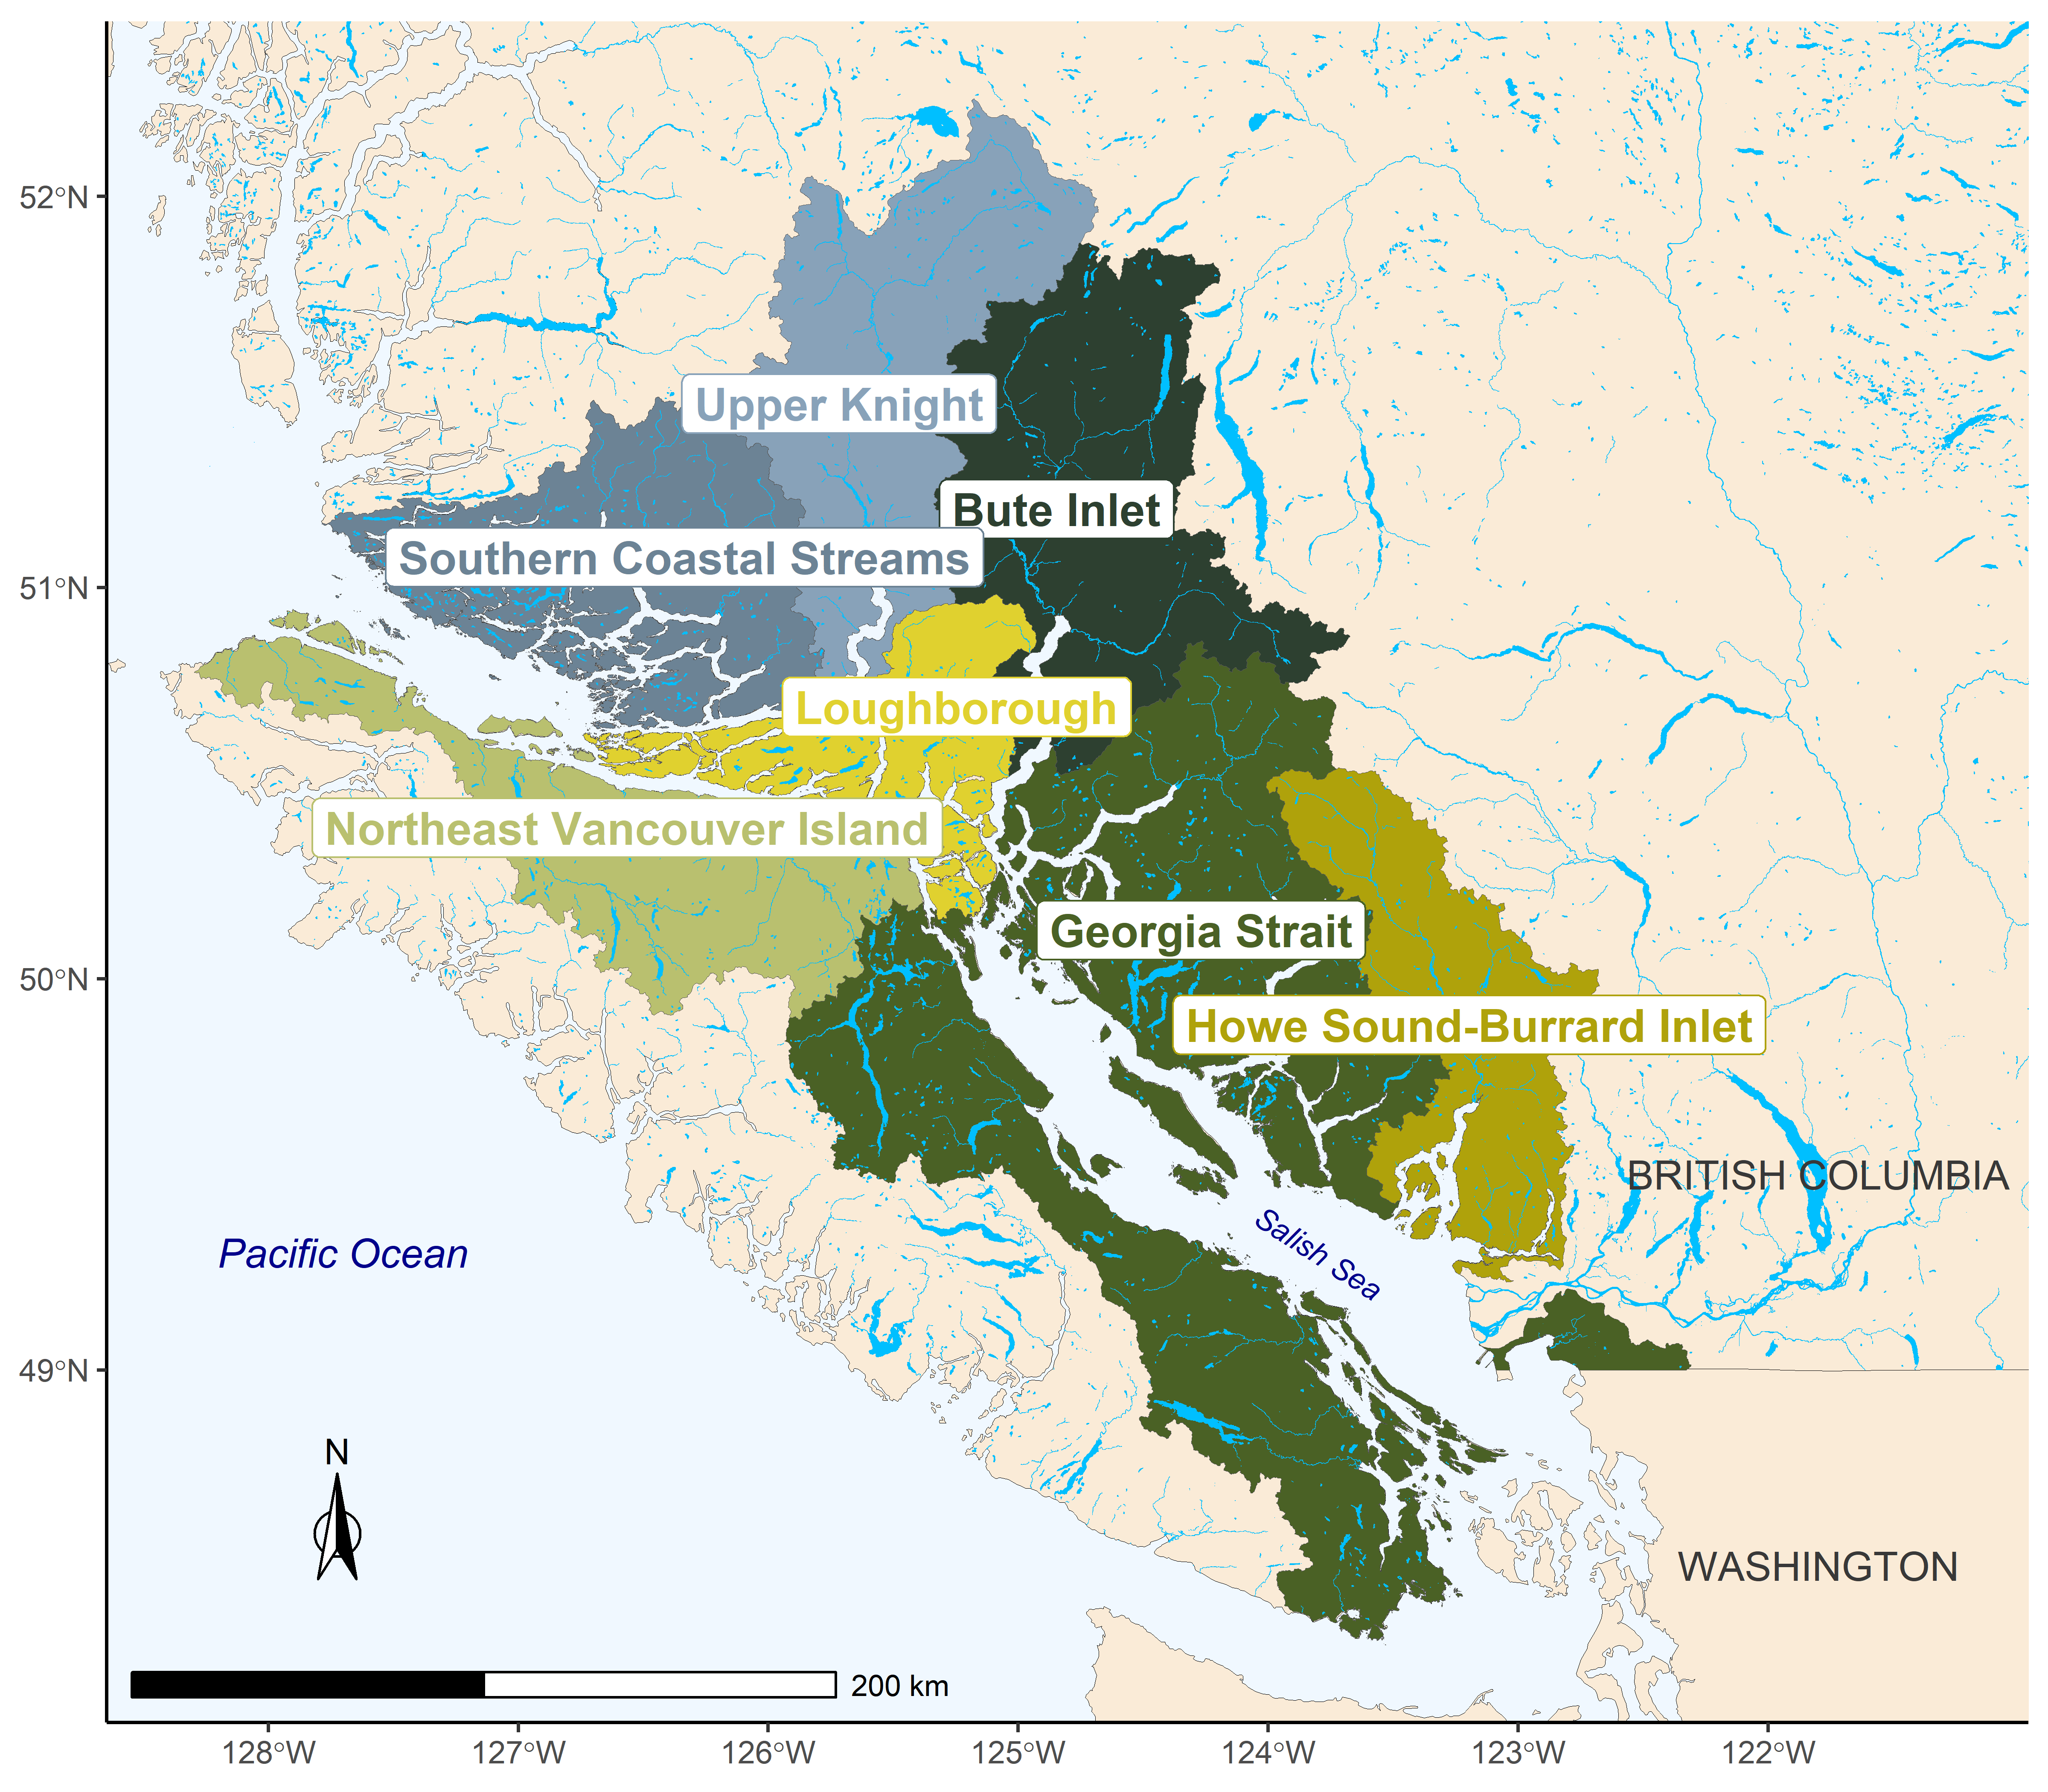
\includegraphics[width=6in]{figure/chum-map}}{Figure \ref{fig:chum-map}} 

}

\caption{The seven Conservation Units that make up the Inside South Coast Chum Stock Management Unit (not including Lower Fraser and Fraser Canyon Conservation Units).}\label{fig:chum-map}
\end{figure}
\hypertarget{data-1}{%
\subsection{DATA}\label{data-1}}

We used the same data used in (\protect\hyperlink{ref-holtEvaluatingBenchmarksBiological2018}{\textbf{holtEvaluatingBenchmarksBiological2018?}}), but updated with five additional years of data. Available data included spawner abundance time series from 1959 - 2018 and corresponding CU-level recruitment estimated from run reconstruction. Spawner abundance series rely heavily on infilling; 60\% of observations (count of spawners for an individual stream, in a given year) were missing and needed to be infilled. Recruitment data are considered highly uncertain for all ISC Chum CUs due to uncertain assumptions required to assign mixed fishery catch to CUs within the run reconstruction model. As a result, we did not consider spawner recruit series to be reliable enough to estimate stock recruitment-based benchmarks such as \(S_{MSY}\) and \(S_{gen}\). We did however use spawner recruit model fits to provide approximate estimates of CU-level productivity, which are used to inform the application of percentile-based benchmarks.

\protect\hyperlink{ref-vanwillInnerSouthCoast2014}{Van Will} (\protect\hyperlink{ref-vanwillInnerSouthCoast2014}{2014}) provides more details on the data sources, infilling procedures and run reconstruction, which were reproduced for this study. We did not include the Lower Fraser or Fraser Canyon chum CUs. More details can be found in Appendix~\ref{app:08-appendix-chum-data}. Note that we removed spawners for the Qualicum River, Little Qualicum River, and Puntledge River (Georgia Strait CU), as these systems have been nearly 100\% enhanced at least since enhancement began at these locations. We made the assumption that these streams had 100\% hatchery origin spawners.

Links to data and analysis code repository are in Appendix~\ref{app:github-appendix}.

\hypertarget{cu-status-estimation-1}{%
\subsection{CU STATUS ESTIMATION}\label{cu-status-estimation-1}}

For this case study, we consider two approaches for characterizing CU status: (1) Pacific Salmon Scanner Tool (or Salmon Scanner) (2) CU-level abundance relative to a percentile lower benchmark

The first approach, which uses the Salmon Scanner developed by the State of the Salmon program (Section~\ref{rapidToolMethods}), is consistent with Canada's WSP and is recommended by Holt et al.~(in review)\footnote{Holt, C. A., K. Holt, L. Warkentin, C. Wor, \ldots{} . Guidelines for Defining Limit Reference Points for Pacific Salmon Stock Management Units. CSAS Res Doc. In review} as the method that should be used to estimate CU status when using the proportional LRP approach. The second approach is presented or a point of comparison with the Salmon Scanner.''

When applying the Salmon Scanner to ISC-NF Chum, we use percentile benchmarks as both upper and lower benchmarks (\ref{fig:decision-tree}). As a result, both of our approaches to CU status estimation depend on percentile-based benchmarks.

Percentile-based benchmarks can be applied to assess status of CUs when other data - like benchmarks based on productivity or habitat - are not available or reliable ((\protect\hyperlink{ref-holtEvaluatingBenchmarksBiological2018}{\textbf{holtEvaluatingBenchmarksBiological2018?}}), \protect\hyperlink{ref-clarkEvaluationPercentileApproach2014}{Clark et al.} (\protect\hyperlink{ref-clarkEvaluationPercentileApproach2014}{2014})). The suitability of percentile benchmarks was evaluated for ISC Chum by (\protect\hyperlink{ref-holtEvaluatingBenchmarksBiological2018}{\textbf{holtEvaluatingBenchmarksBiological2018?}}), who tested how well percentile benchmarks matched benchmarks from stock-recruit parameters, using retrospective and simulation analyses. (\protect\hyperlink{ref-holtEvaluatingBenchmarksBiological2018}{\textbf{holtEvaluatingBenchmarksBiological2018?}}) also calculated benchmarks based on stock-recruit model parameters for ISC Chum stocks, but did not recommend them due to uncertainty in spawner and recruit data. They tested how well a 25\% percentile benchmark (and higher values up to 50\%) compared to estimates of \(S_{gen}\) for these CUs. They found that percentile benchmarks (from 25-50\%) under moderate to high harvest rates and low to moderate productivity tended to underestimate `true' \(S_{gen}\) values (estimated from the same data), which would lead to optimistic and incorrect status assessments. More work on alternatives to percentile benchmarks were needed in this case.

For this case study, percentile benchmarks were calculated using the infilled escapement time series (not smoothed) and status for year \(i\) was determined by comparing the geometric mean (4 year window, ending with year \(i\)) with the benchmark.

\renewcommand*{\arraystretch}{1.5}
\begin{table}[ht]
\centering
\caption{Selected percentile-based lower and upper benchmarks identified to be similar or higher in value than stock-recruitment based benchmarks under the WSP, along gradients in productivity (recruits/spawner) and average harvest rates. * denotes the low-productivity scenario where lower and upper Ricker-based benchmarks are very close to one another, resulting in lower and upper percentile-based benchmarks that are the same. From Holt et al. 2018.}
\begin{tabular}{l l p{2.5cm} p{2.5cm} p{2.5cm}}
\hline       &     & \multicolumn{3}{l}{Harvest rate}\\ 
& & <20\% & 20-40\% & 40-60 \% \\
\hline
Productivity& >4 & 25th (lower)  50th (upper) & 25th (lower) 50th (upper) & 25th (lower) 50th (upper) \\
& 2.5-4 & 25th (lower) 50th (upper) & 25th (lower) 50th (upper) & Further evaluation required \\
& 1.5-2.5 & *50th (lower and upper) & Further evaluation required & Further evaluation required \\               
\hline
\end{tabular}
\label{tab:holt-tab6}
\end{table}
(\protect\hyperlink{ref-holtEvaluatingBenchmarksBiological2018}{\textbf{holtEvaluatingBenchmarksBiological2018?}}) recommended different percentiles to be used based on Ricker \(\alpha\) and average harvest rate (figure~\ref{tab:holt-tab6}). Based on these recommendations, Georgia Strait and Howe Sound Burrard Inlet fall in the category of using 25\textsuperscript{th} percentile as a lower benchmark and 50\% as an upper benchmark (Ricker \(\alpha\) 2.5-4, harvest rate 20-40\%). Loughborough, Northeast Vancouver Island, and Upper Knight (\(\alpha\) 1.5-2.5 and harvest rate 0-20\%) had a 50\textsuperscript{th} percentile lower and upper benchmark recommended. Bute Inlet (\(\alpha\) 1.5-2.5, harvest rate 20-40\%) needed further evaluation and percentile benchmarks were not recommended. Percentile benchmarks were also not recommended for Southern Coastal Streams due to low productivity (\(\alpha\) \textless1.5). Thus, we used 25\% of spawner abundance as a lower benchmark for Georgia Strait and Howe Sound Burrard Inlet, 50\% for Loughborough, Northeast Vancouver Island, Upper Knight, and did not use percentile benchmarks for Bute Inlet and Southern Coastal Streams (Table~\ref{tab:CU-summary}).

The methods for applying the Salmon Scanner to get CU status is described in Chapter (\protect\hyperlink{ref-ref}{\textbf{ref?}})(\#MethodsChapter). In applying the Salmon Scanner to ISC Chum, we used the percentile benchmarks as recommended in (\protect\hyperlink{ref-holtEvaluatingBenchmarksBiological2018}{\textbf{holtEvaluatingBenchmarksBiological2018?}}) for lower and upper benchmarks for the five CUs that have appropriate percentiles benchmarks identified (as described above). For Bute Inlet and Southern Coastal Streams, we did not use benchmarks. When benchmarks are not available, trends were used to assess status according to the decision tree (Fig.~\ref{fig:decision-tree}).

\hypertarget{lrp-estimation-proportion-of-cus-1}{%
\subsection{LRP ESTIMATION: PROPORTION OF CUs}\label{lrp-estimation-proportion-of-cus-1}}

\hypertarget{methods-4}{%
\subsubsection{Methods}\label{methods-4}}

We looked at the proportion of CUs that had status estimates above the red zone (or, above the lower percentile benchmark) to determine in which years between 1960 and 2018 the LRP would have been breached. As with the Interior Fraser Coho and WCVI Chinook case studies, we required all CUs to be above the red zone for the ISC-NF Chum SMU to be classified as being above the LRP.

The single-metric approach to assessing CU status based on percentiles has specific data requirements ((\protect\hyperlink{ref-holtEvaluatingBenchmarksBiological2018}{\textbf{holtEvaluatingBenchmarksBiological2018?}})) while the Salmon Scanner approach can be applied to any CU with at least a consistent time-series of spawner abundances. To compare LRPs based on CU assessment from these two approaches we compared data subsets including those that used the same data for each method, and all appropriate data for each method. We evaluated six different combinations of data and LRP methods (Table~\ref{tab:LRP-scenarios}). For this comparison, we used percentile benchmarks based on (\protect\hyperlink{ref-holtEvaluatingBenchmarksBiological2018}{\textbf{holtEvaluatingBenchmarksBiological2018?}}). The benchmarks were estimated using the entire time series. `Full' scenarios only included CUs with complete time series (no CUs with years with CU-level infilling). `Partial' scenarios included CUs with incomplete time series, where the years that did not have observations in those CUs were omitted.

For scenarios 1 and 2, we used CU status based on percentile benchmarks that are determined by productivity and historical exploitation outlined in (\protect\hyperlink{ref-holtEvaluatingBenchmarksBiological2018}{\textbf{holtEvaluatingBenchmarksBiological2018?}}) (Table~\ref{tab:LRP-scenarios}). This method used the annual escapement values to calculate the benchmarks and the generational mean (geometric mean of 4 years) of escapement for year \(i\) and previous three years to assess status in year \(i\). Scenario 1 includes the four CUs which had complete time series (observations in each year, no CU-level infilling required) and that also had appropriate percentile benchmarks based on (\protect\hyperlink{ref-holtEvaluatingBenchmarksBiological2018}{\textbf{holtEvaluatingBenchmarksBiological2018?}}). For example, Upper Knight was excluded because it did not have a complete time series, Southern Coastal Streams was excluded because it does not have an appropriate percentile benchmark, and Bute Inlet was excluded for both of these reasons. We then relaxed this assumption and included all CUs that meet the constraints of (\protect\hyperlink{ref-holtEvaluatingBenchmarksBiological2018}{\textbf{holtEvaluatingBenchmarksBiological2018?}}) even if they had missing data for some years (Scenario 2). This scenario included Upper Knight in some years, which meant that it had five CUs in some years and four in others. Thus, the power to detect red status varied among years in Scenario 2, using more of the available data than Scenario 1. For scenarios 3-6, we used status based on the Salmon Scanner. To compare results between status from percentiles and the Salmon Scanner, we used the Salmon Scanner on the same two data sets we used for percentiles. Scenarios 3 and 1 have the same data, and Scenarios 2 and 6 have the same data. Because the Salmon Scanner does not need benchmarks (percentile or otherwise) to assign status, it could also be used for CUs that did not have appropriate percentile benchmarks (Southern Coastal Streams and Bute Inlet). Scenario 4 only included CUs with a full time series, and Scenario 5 included Upper Knight and Bute Inlet, which had some missing years.

\renewcommand*{\arraystretch}{1.5}
\begin{table}[ht]
\centering
\caption{Scenarios using different subsets of data (CU names abbreviated) and methods to assign LRP status. 'Y' indicates a full time series, 'YP' indicates a time series was included but is partial (missing years that required CU-level infilling which wer omitted). Bute Inlet and Southern Coastal Streams do not have appropriate percentile benchmarks. 'Full' scenarios use only years with full time series (no CU-level infilled CUs) and 'partial' scenarios include CU-level infilled CUs but drop years with CU-level infilling for those CUs.}
\begin{tabular}{l c c c c c c c }
\hline    
Scenario Name &   \rotatebox{90}{Southern Coastal Streams} &   \rotatebox{90}{ North East Vancouver Island} &  \rotatebox{90}{ Upper Knight} &  \rotatebox{90}{ Loughborough} &  \rotatebox{90}{ Bute Inlet} & \rotatebox{90}{ Georgia Strait} & \rotatebox{90}{ Howe Sound-Burrard Inlet}\\ 
\hline
1. Percentile- 4 CUs full       & - & Y & -  & Y & -  & Y & Y \\
2. Percentile- 5 CUs partial    & - & Y & YP & Y & -  & Y & Y \\
3. Decision Tree- 4 CUs full    & - & Y & -  & Y & -  & Y & Y \\
4. Decision Tree- 5 CUs full    & Y & Y & -  & Y & -  & Y & Y \\
5. Decision Tree- 7 CUs partial & Y & Y & YP & Y & YP & Y & Y \\
6. Decision Tree- 5 CUs partial & - & Y & YP & Y & -  & Y & Y \\
\hline
\end{tabular}
\label{tab:LRP-scenarios}
\end{table}
\hypertarget{results-3}{%
\subsubsection{Results}\label{results-3}}

\textbf{CU Status Based on Salmon Scanner}

Using this method, two out of five CUs with data in the most recent year of data (2018) would be above their lower benchmark (amber or green zone) and 3 would be below (red zone). Over the time series, status for Howe Sound-Burrard Inlet and Georgia Strait has improved, while status in other CUs has declined or switched from green to red several times.
\begin{figure}[htb]

{\centering \pdftooltip{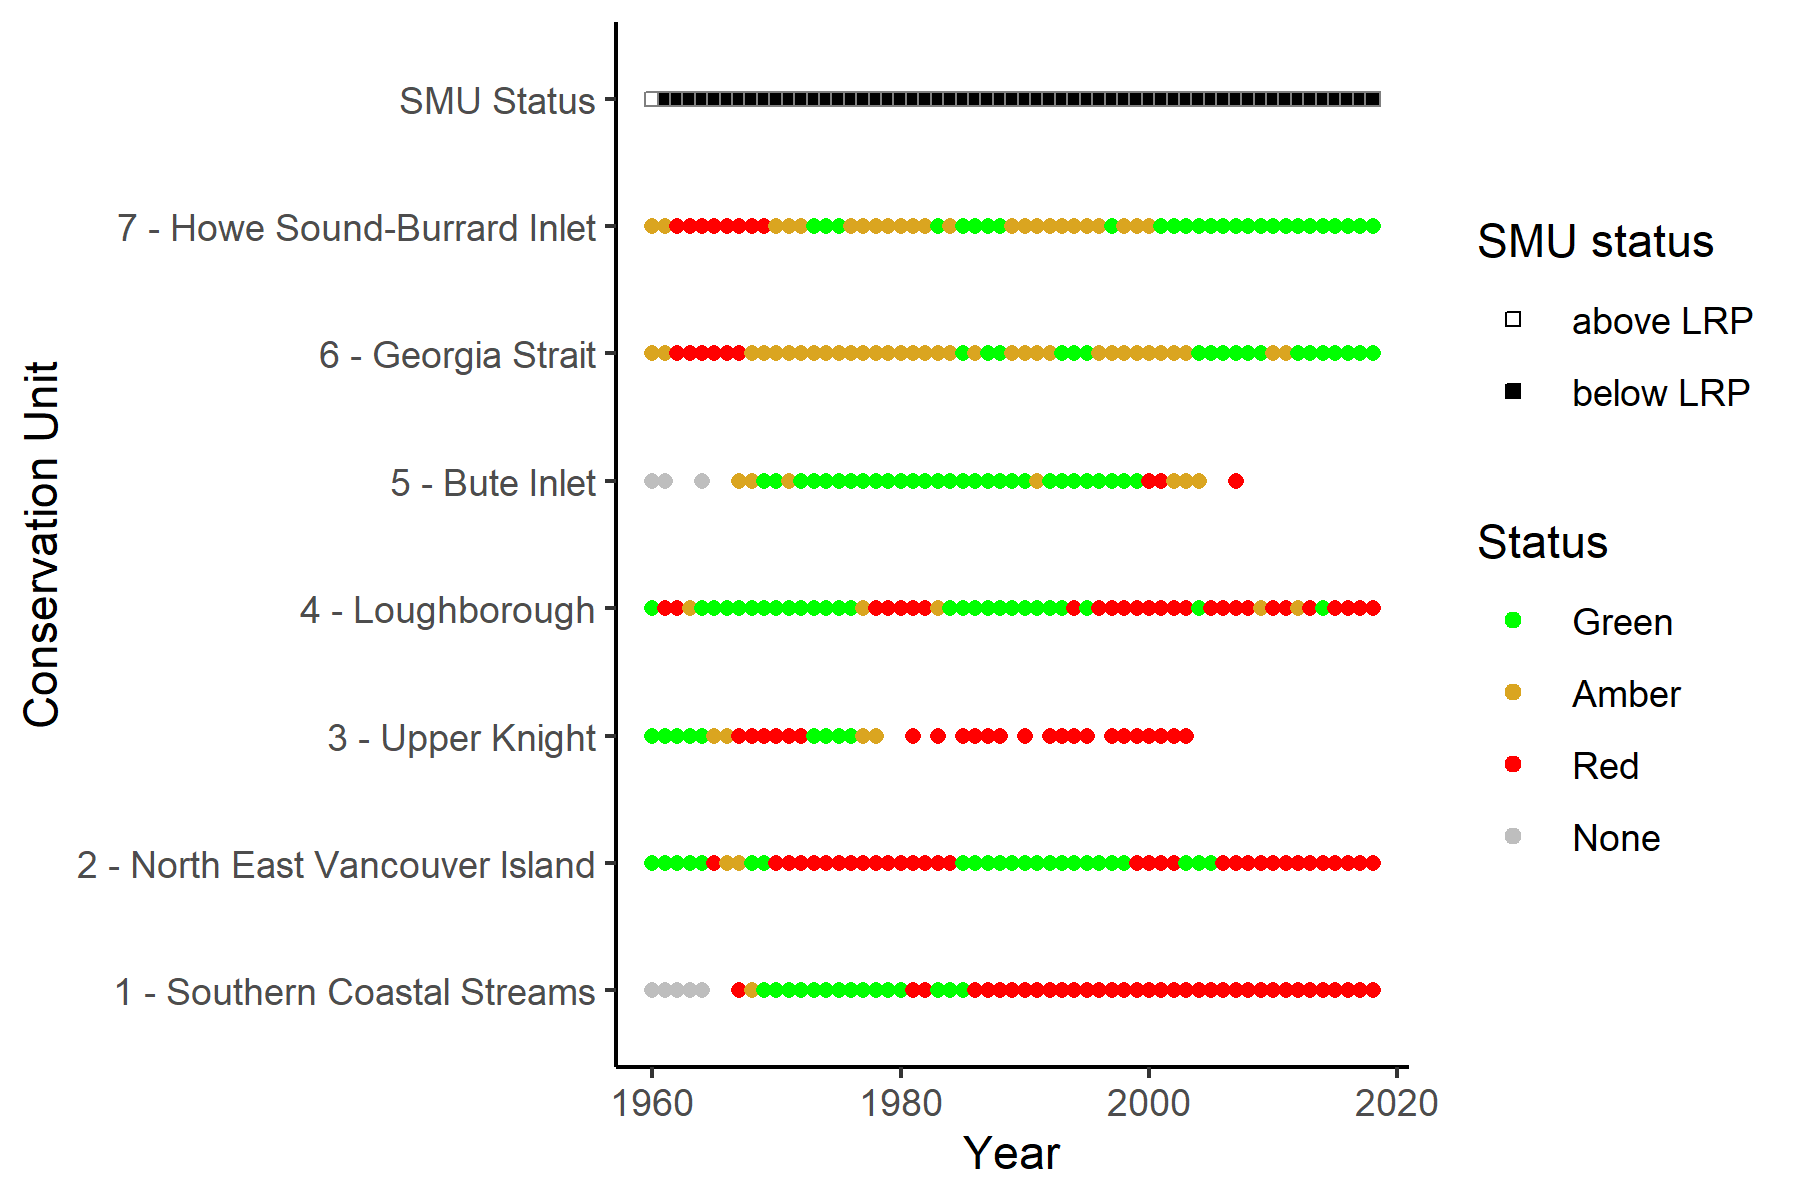
\includegraphics[width=6in]{figure/fig_status_by_CU_perc_RelAbd}}{Figure \ref{fig:chum-CU-status-tree}} 

}

\caption{Status of CUs based on multi-dimensional status assessment (decision tree). Years with CU-level infilling were not included.}\label{fig:chum-CU-status-tree}
\end{figure}
\textbf{CU Status Based on Percentile Benchmarks}

Two out of four CUs were below their percentile lower benchmark in 2018 (Figure~\ref{fig:chum-perc-status-static}. Howe Sound-Burrard Inlet and Georgia Strait had status above their lower benchmarks.

In supplementary analyses, we evaluated percentile benchmarks retrospectively for each year in time series using only data prior to that year. As more years of data were included, percentile benchmarks increased over time for Georgia Strait (especially the 50\textsuperscript{th} percentile) and had modest increases for Howe Sound-Burrard Inlet (Figure~\ref{fig:chum-perc-retro}). Percentile benchmarks decreased by a small amount for Loughborough and North East Vancouver Island.

Among these three CUs, Southern Coastal Streams and Upper Knight show evidence of shifting baselines if percentile approaches are used.
\begin{figure}[htb]

{\centering \pdftooltip{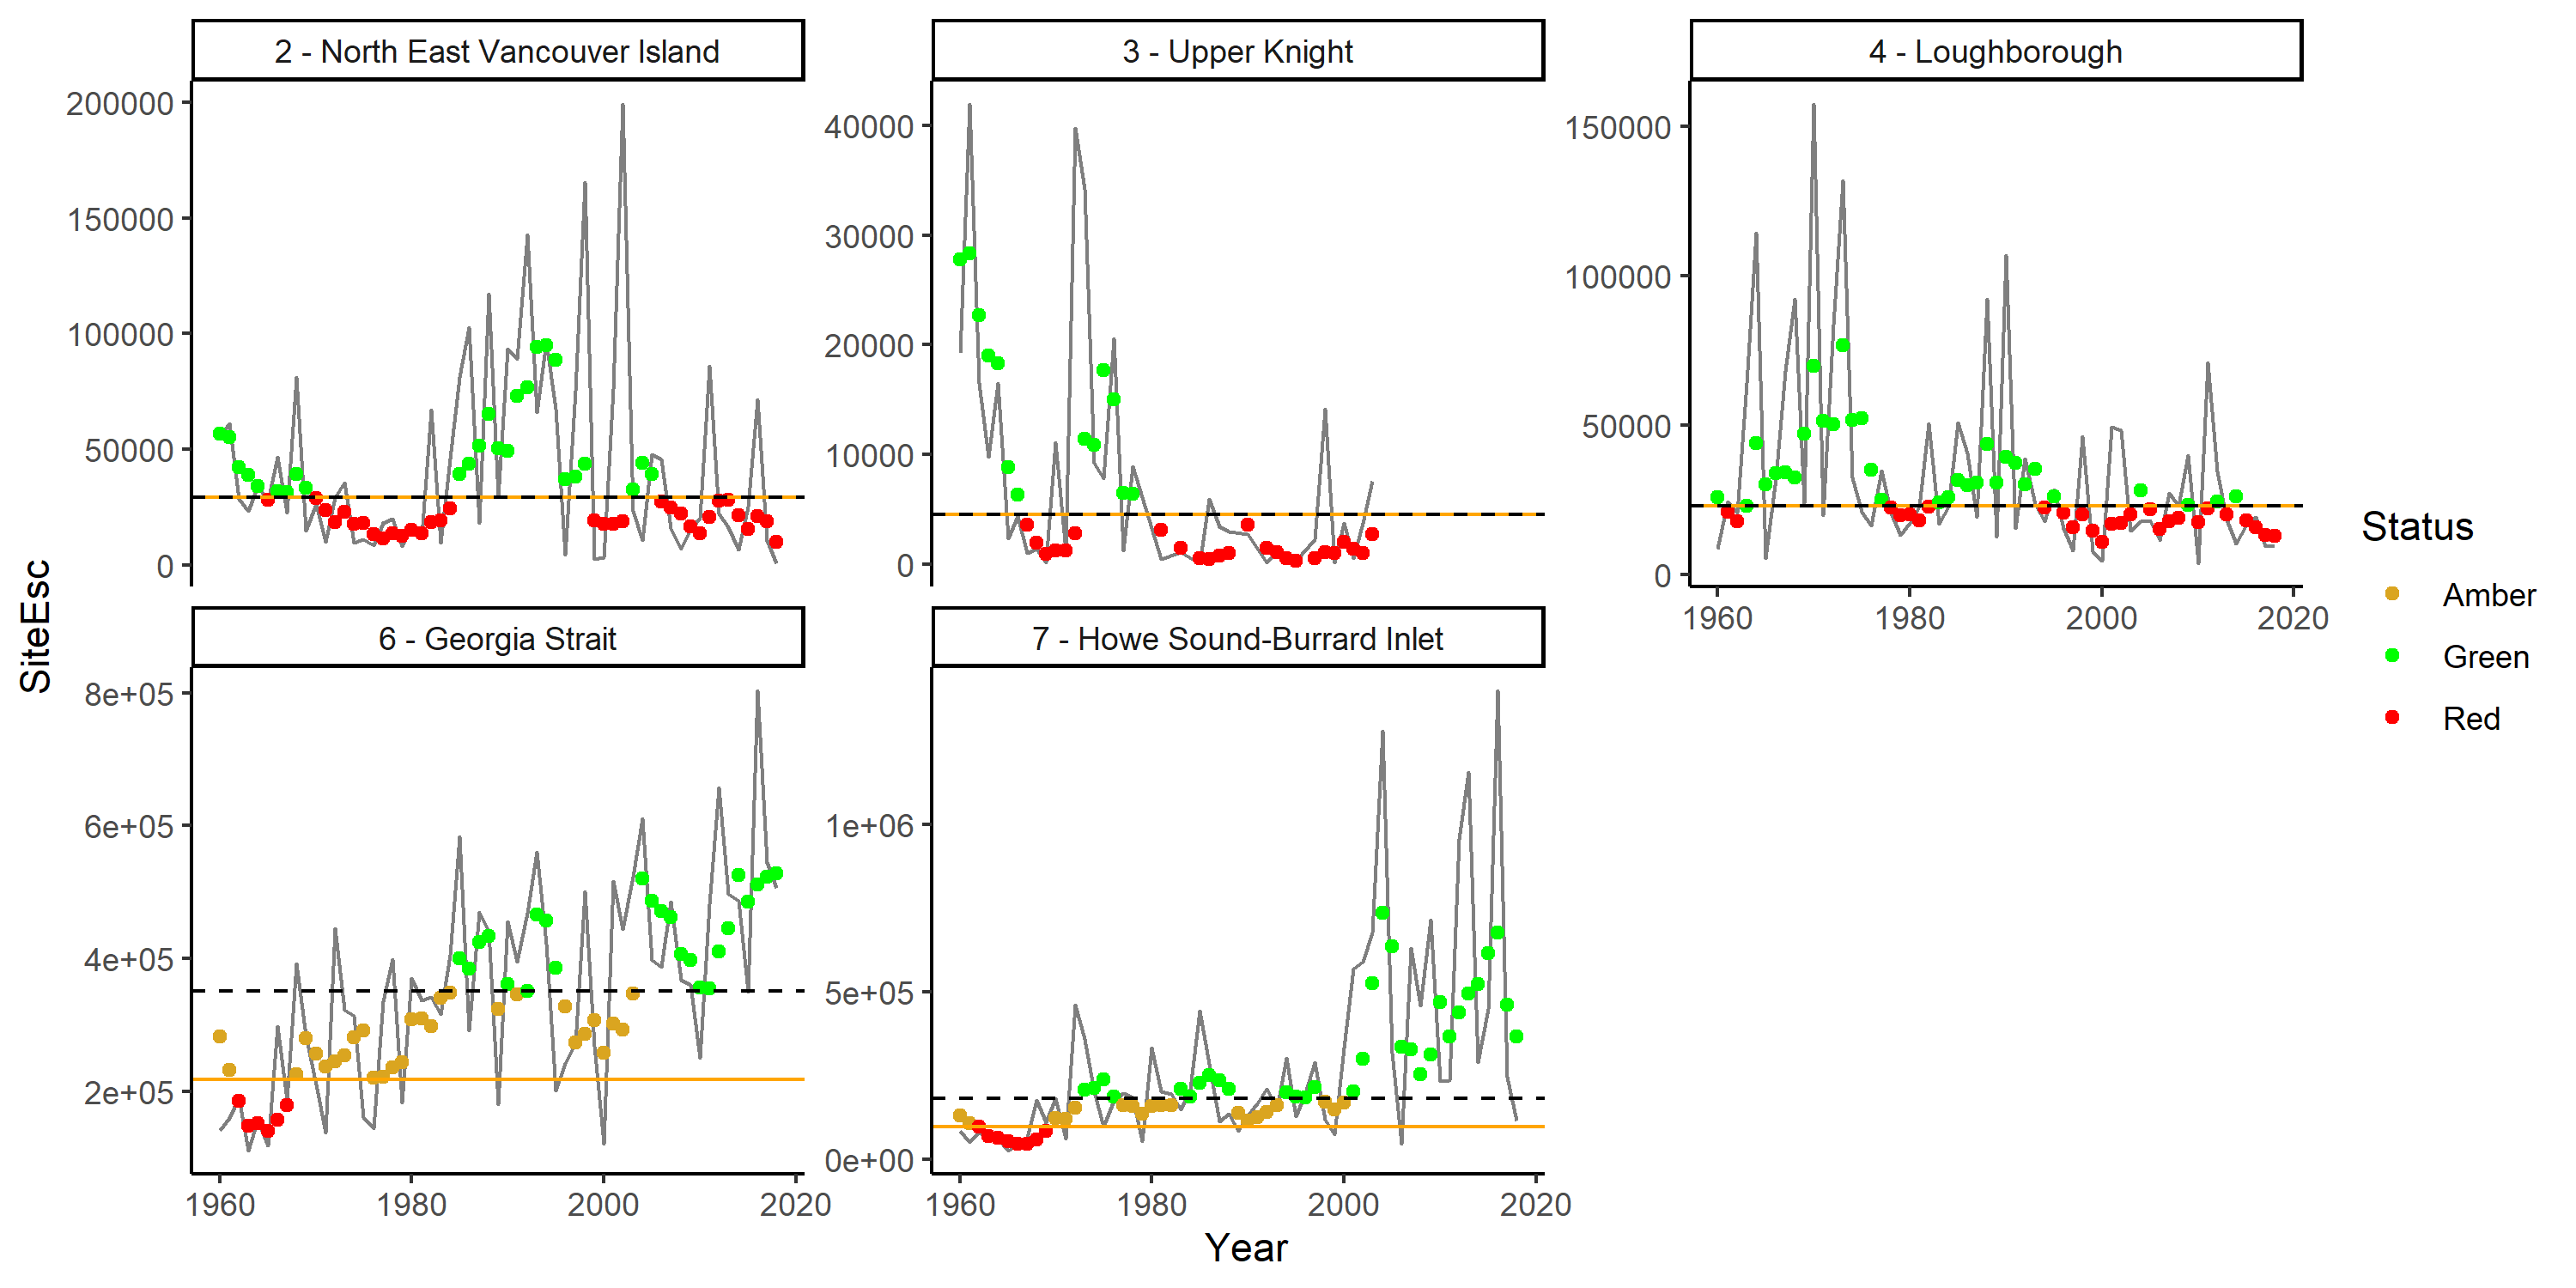
\includegraphics[width=6in]{figure/fig_percentile_bm_rel_abd}}{Figure \ref{fig:chum-perc-status-static}} 

}

\caption{Spawner escapement (solid black line) with generational mean (4 year rolling geometric mean) of escapement in points.}\label{fig:chum-perc-status-static}
\end{figure}
\#\#LRP ESTIMATION: AGGREGATE ABUNDANCE LOGISTIC REGRESSION LRPS

\hypertarget{methods-5}{%
\subsubsection{Methods}\label{methods-5}}

We evaluated whether the proportion of CUs above their lower benchmark could be predicted by aggregate abundance using logistic regression models. We tested this using percentile and \(S_{gen}\) benchmarks. These methods used 5 CUs with over 50 years of data (Bute Inlet and Upper Knight both had CU-level infilling in recent years and thus were left out of this analysis).

These methods were applied retrospectively. For a series of years up to a given year, the benchmarks and logistic regressions were calculated with all years up to that year. This was done for all successive years to see how the LRP (and benchmarks, and underlying stock-recruit parameters) would have changed over time as more data was collected.

Due to poor logistic model fits using the entire 1953-2018 time series for both \(S_{gen}\) and percentile benchmarks, we did not conduct full retrospective analyses of logistic-regression based LRPs for this SMU as was completed for the Interior Fraser River Coho case study. The characteristics of the data that led to poor logistic model fits are highlighted in the results section below.

Projection-based LRPs are an alternative aggregate-abundance LRP that we did not consider for this SMU due to lack of peer-reviewed stock-recruitment model fits for component CUs. However, this approach could be considered in future analyses given consensus on model structure and parameterization that provide realistic uncertainties in projections of population dynamics.

\hypertarget{results-4}{%
\subsubsection{Results}\label{results-4}}

The logistic models predicting whether all CUs were above their benchmark based on aggregate abundance fit the data poorly (Figures~\ref{fig:chum-logistic-sgen},~\ref{fig:chum-logistic-perc}). In both cases, the sum of abundance for all CUs in a given year was not a good predictor of whether those CUs were above their benchmarks in that year. Years with high aggregate abundance but with some CUs below their benchmark make a logistic model unsuitable for the purpose of estimating which aggregate abundance is linked to a high probability of each component CU being above its lower benchmark. Note that these regressions used the aggregate abundance of only the CUs used in the regressions, and excluded the other CUs.

Percentile approaches were not used for the other three CUs for the purpose of the logistic regression of aggregate abundance because they were not appropriate based on productivity and harvest rates (see (\protect\hyperlink{ref-holtEvaluatingBenchmarksBiological2018}{\textbf{holtEvaluatingBenchmarksBiological2018?}}) Table 6), CU-level infilling, or both (although they are shown in Figure~\ref{fig:chum-perc-retro}).

The diagnostics for the logistic regression indicated that the model fit was poor for percentile benchmarks (Table~\ref{tab:logistic-diag-chum}, Figure~\ref{fig:chum-logistic-perc}). Pseudo \(R^2\) was low (0.03), indicating that the fit is not good. The Box-Tidwell test (p-value = 0.02) indicated a significant lack of linearity in the relationship between aggregate abundance and log-odds, which means that the assumption that the relationship between aggregate abundance and log-odds is linear was not met. There was not a significant improvement in the model fit when aggregate abundance was included, compared to the null model based on a Goodness of fit p value of 0.13 (\textgreater0.05), indicating that there is not significant improvement in fit with the variable (aggregate abundance). There was no evidence of outliers, and there was a sufficient sample size. The ratio of correct classification based on a confusion matrix was 0.7. Note that this method tends to have overly optimistic values. The Wald p-value was not significant for \(B_{1}\) (0.019), the coefficient for aggregate abundances. There was no evidence for autocorrelation in residuals. Regressions based on \(S_{gen}\) had similarly poor model fits (Figure~\ref{fig:chum-logistic-sgen}.
\begin{figure}[htb]

{\centering \pdftooltip{\includegraphics[width=6in]{figure/chum-logistic-perc}}{Figure \ref{fig:chum-logistic-perc}} 

}

\caption{Logistic regression of whether escapement of all component CUs were above their percentile benchmarks based on aggregate abundance, for Inside South Coast Chum SMU. Includes CUs where percentile benchmarks were appropriate (no Bute Inlet, Upper Knight, or Southern Coastal Streams)}\label{fig:chum-logistic-perc}
\end{figure}
\begin{longtable}[]{@{}
  >{\raggedright\arraybackslash}p{(\columnwidth - 2\tabcolsep) * \real{0.36}}
  >{\raggedright\arraybackslash}p{(\columnwidth - 2\tabcolsep) * \real{0.21}}@{}}
\caption{\label{tab:logistic-diag-chum} Model diagnostic statistics from logistic regression LRP using percentile benchmarks. A description of diagnostic tests is provided in Section 2. Hit ratios are shown for p=0.5.}\tabularnewline
\toprule
\begin{minipage}[b]{\linewidth}\raggedright
Diagnostic Test
\end{minipage} & \begin{minipage}[b]{\linewidth}\raggedright
Value
\end{minipage} \\
\midrule
\endfirsthead
\toprule
\begin{minipage}[b]{\linewidth}\raggedright
Diagnostic Test
\end{minipage} & \begin{minipage}[b]{\linewidth}\raggedright
Value
\end{minipage} \\
\midrule
\endhead
Box-Tidwell p-value & 0.02 \\
Max. deviance residual & 1.69 \\
AR-1 & 0.14 \\
Wald p-value & 0.19 \\
Goodness-of-fit p-value & 0.13 \\
Pseudo-\(R^2\) & 0.03 \\
Hit Ratio (p= 50\%) & 0.7 \\
\bottomrule
\end{longtable}
Several factors led to these poor model fits. The Inside South Coast Chum SMU is made up of seven CUs that vary in their escapement abundance. In many years, escapement in Georgia Strait and Howe Sound-Burrard Inlet is greater than in other CUs by two orders of magnitude (Fig.~\ref{fig:chum-spawner-distribution}). In addition, the correlation in escapement among these seven CUs is low (Fig.~\ref{fig:chum-spawner-corr}). These characteristics mean that the aggregate abundance may be high due to one or more CUs with high escapements, while one more smaller CUs are below their benchmark. High aggregate escapements do not mean that all CUs are above their benchmark. This makes sense because this SMU covers a large area with many different populations affected by both local and regional factors. These seven CUs also have different numbers of populations. There are also differences in actual productivity (recruits per spawner) among CUs.
\begin{figure}[htb]

{\centering \pdftooltip{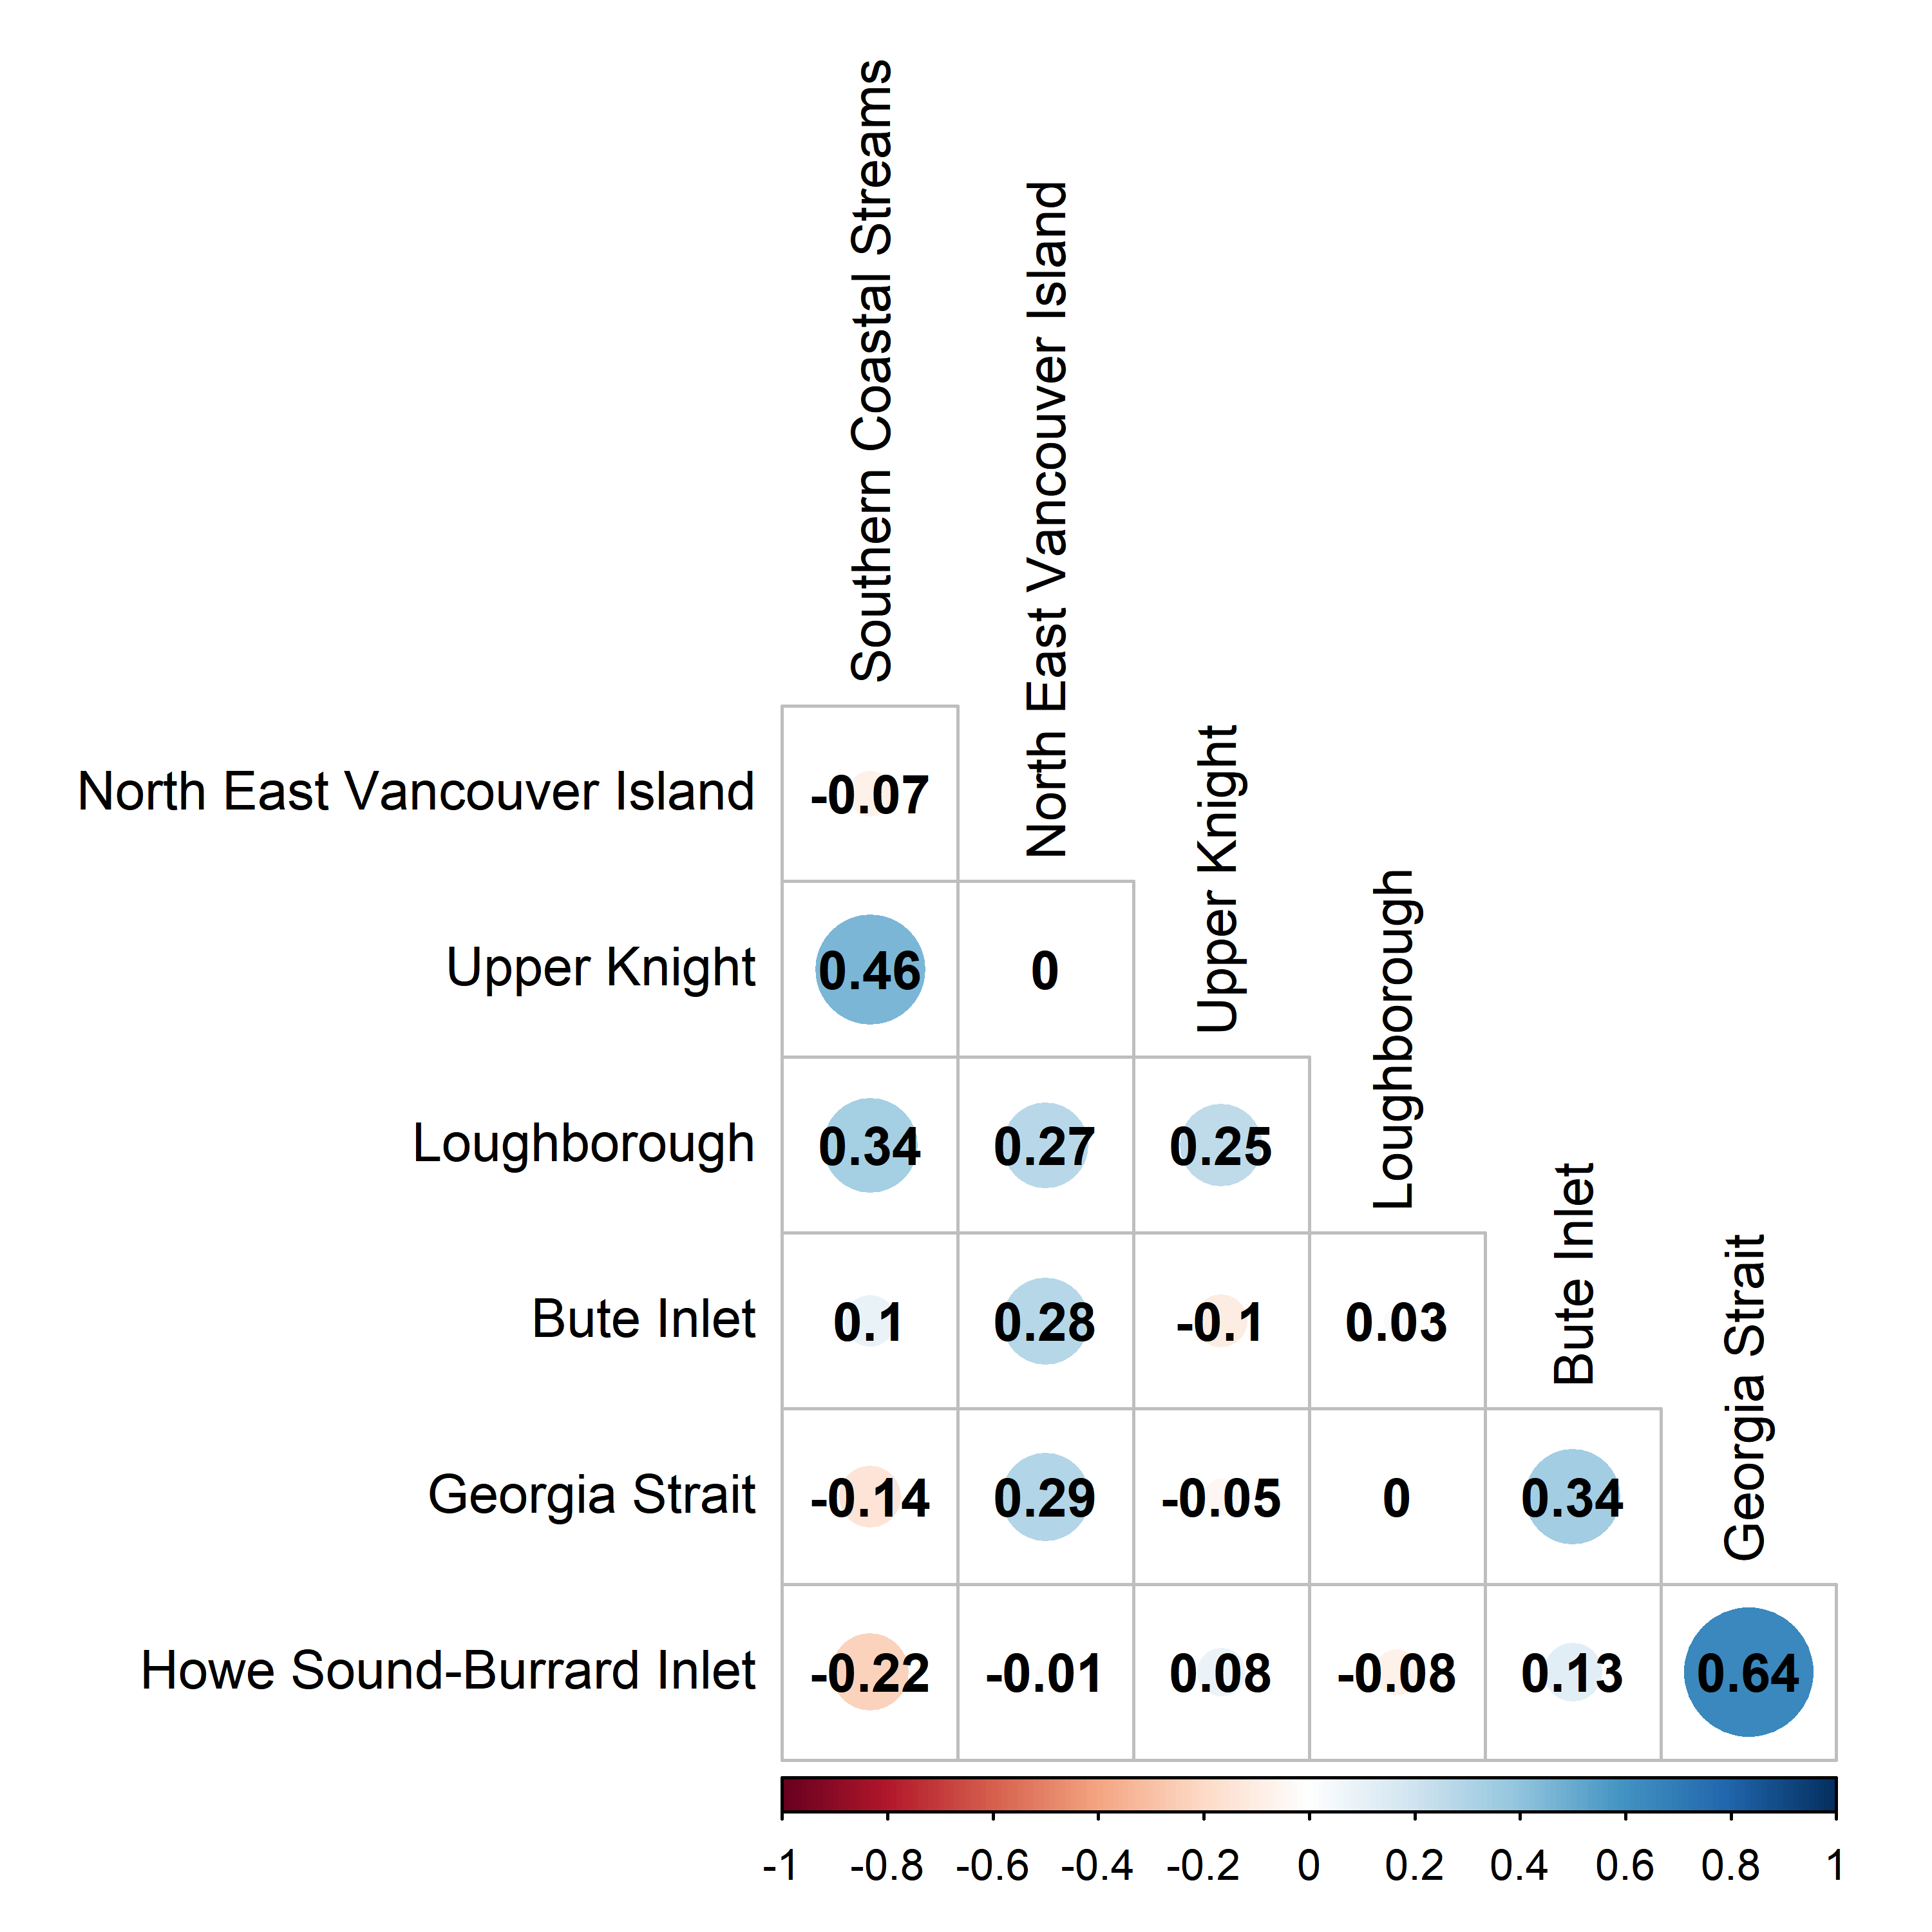
\includegraphics[width=6in]{figure/chum-spawners-corr}}{Figure \ref{fig:chum-spawner-corr}} 

}

\caption{Pairwise correlations of spawner abundance between Inside South Coast Chum Conservation Units.}\label{fig:chum-spawner-corr}
\end{figure}
\hypertarget{historical-evaluation-of-status-across-lrp-methods-2}{%
\subsection{HISTORICAL EVALUATION OF STATUS ACROSS LRP METHODS}\label{historical-evaluation-of-status-across-lrp-methods-2}}

LRP status based on percentile benchmarks had more years below the LRP Salmon Scanner status (Figure~\ref{fig:chum-LRP-compare}, Table~\ref{tab:LRP-scenarios}). Comparing scenarios 1 and 3 (same data) in a given year, ISC Chum were below the LRP based on percentile benchmarks but above it based on decision tree. Scenarios 2 and 6 (same data, more data than 1 and 3) show a similar pattern.

In this case study, adding more data changed the number of years that the SMU was below the LRP. Scenario 5 (most data) had the most years below the LRP. Comparing scenarios 1 and 2, which are both based on percentile benchmarks, including more data (scenario 2) results in more years below the LRP. Comparing scenarios 4 and 5 (decision tree only), including more observations results in one year switching from above the LRP to below it. Comparing scenarios 5 and 6 (where scenario 6 had two fewer CUs than scenario 5), including the two CUs in scenario 5 results in three years switching from above the LRP to below . Other applications may result in different outcomes of including more data based on the status of additional CUs or years.

We found that SMU status can be below the LRP even if the aggregate abundance increases. For ISC Chum, this is mainly due to years with high abundances of Georgia Strait and Burrard Inlet-Howe Sound and low abundances and red status in other, smaller CUs, such as Southern Coastal Streams. This highlights the importance of including a metrics of status at the CU level, which influence the overall SMU status.
\begin{figure}[htb]

{\centering \pdftooltip{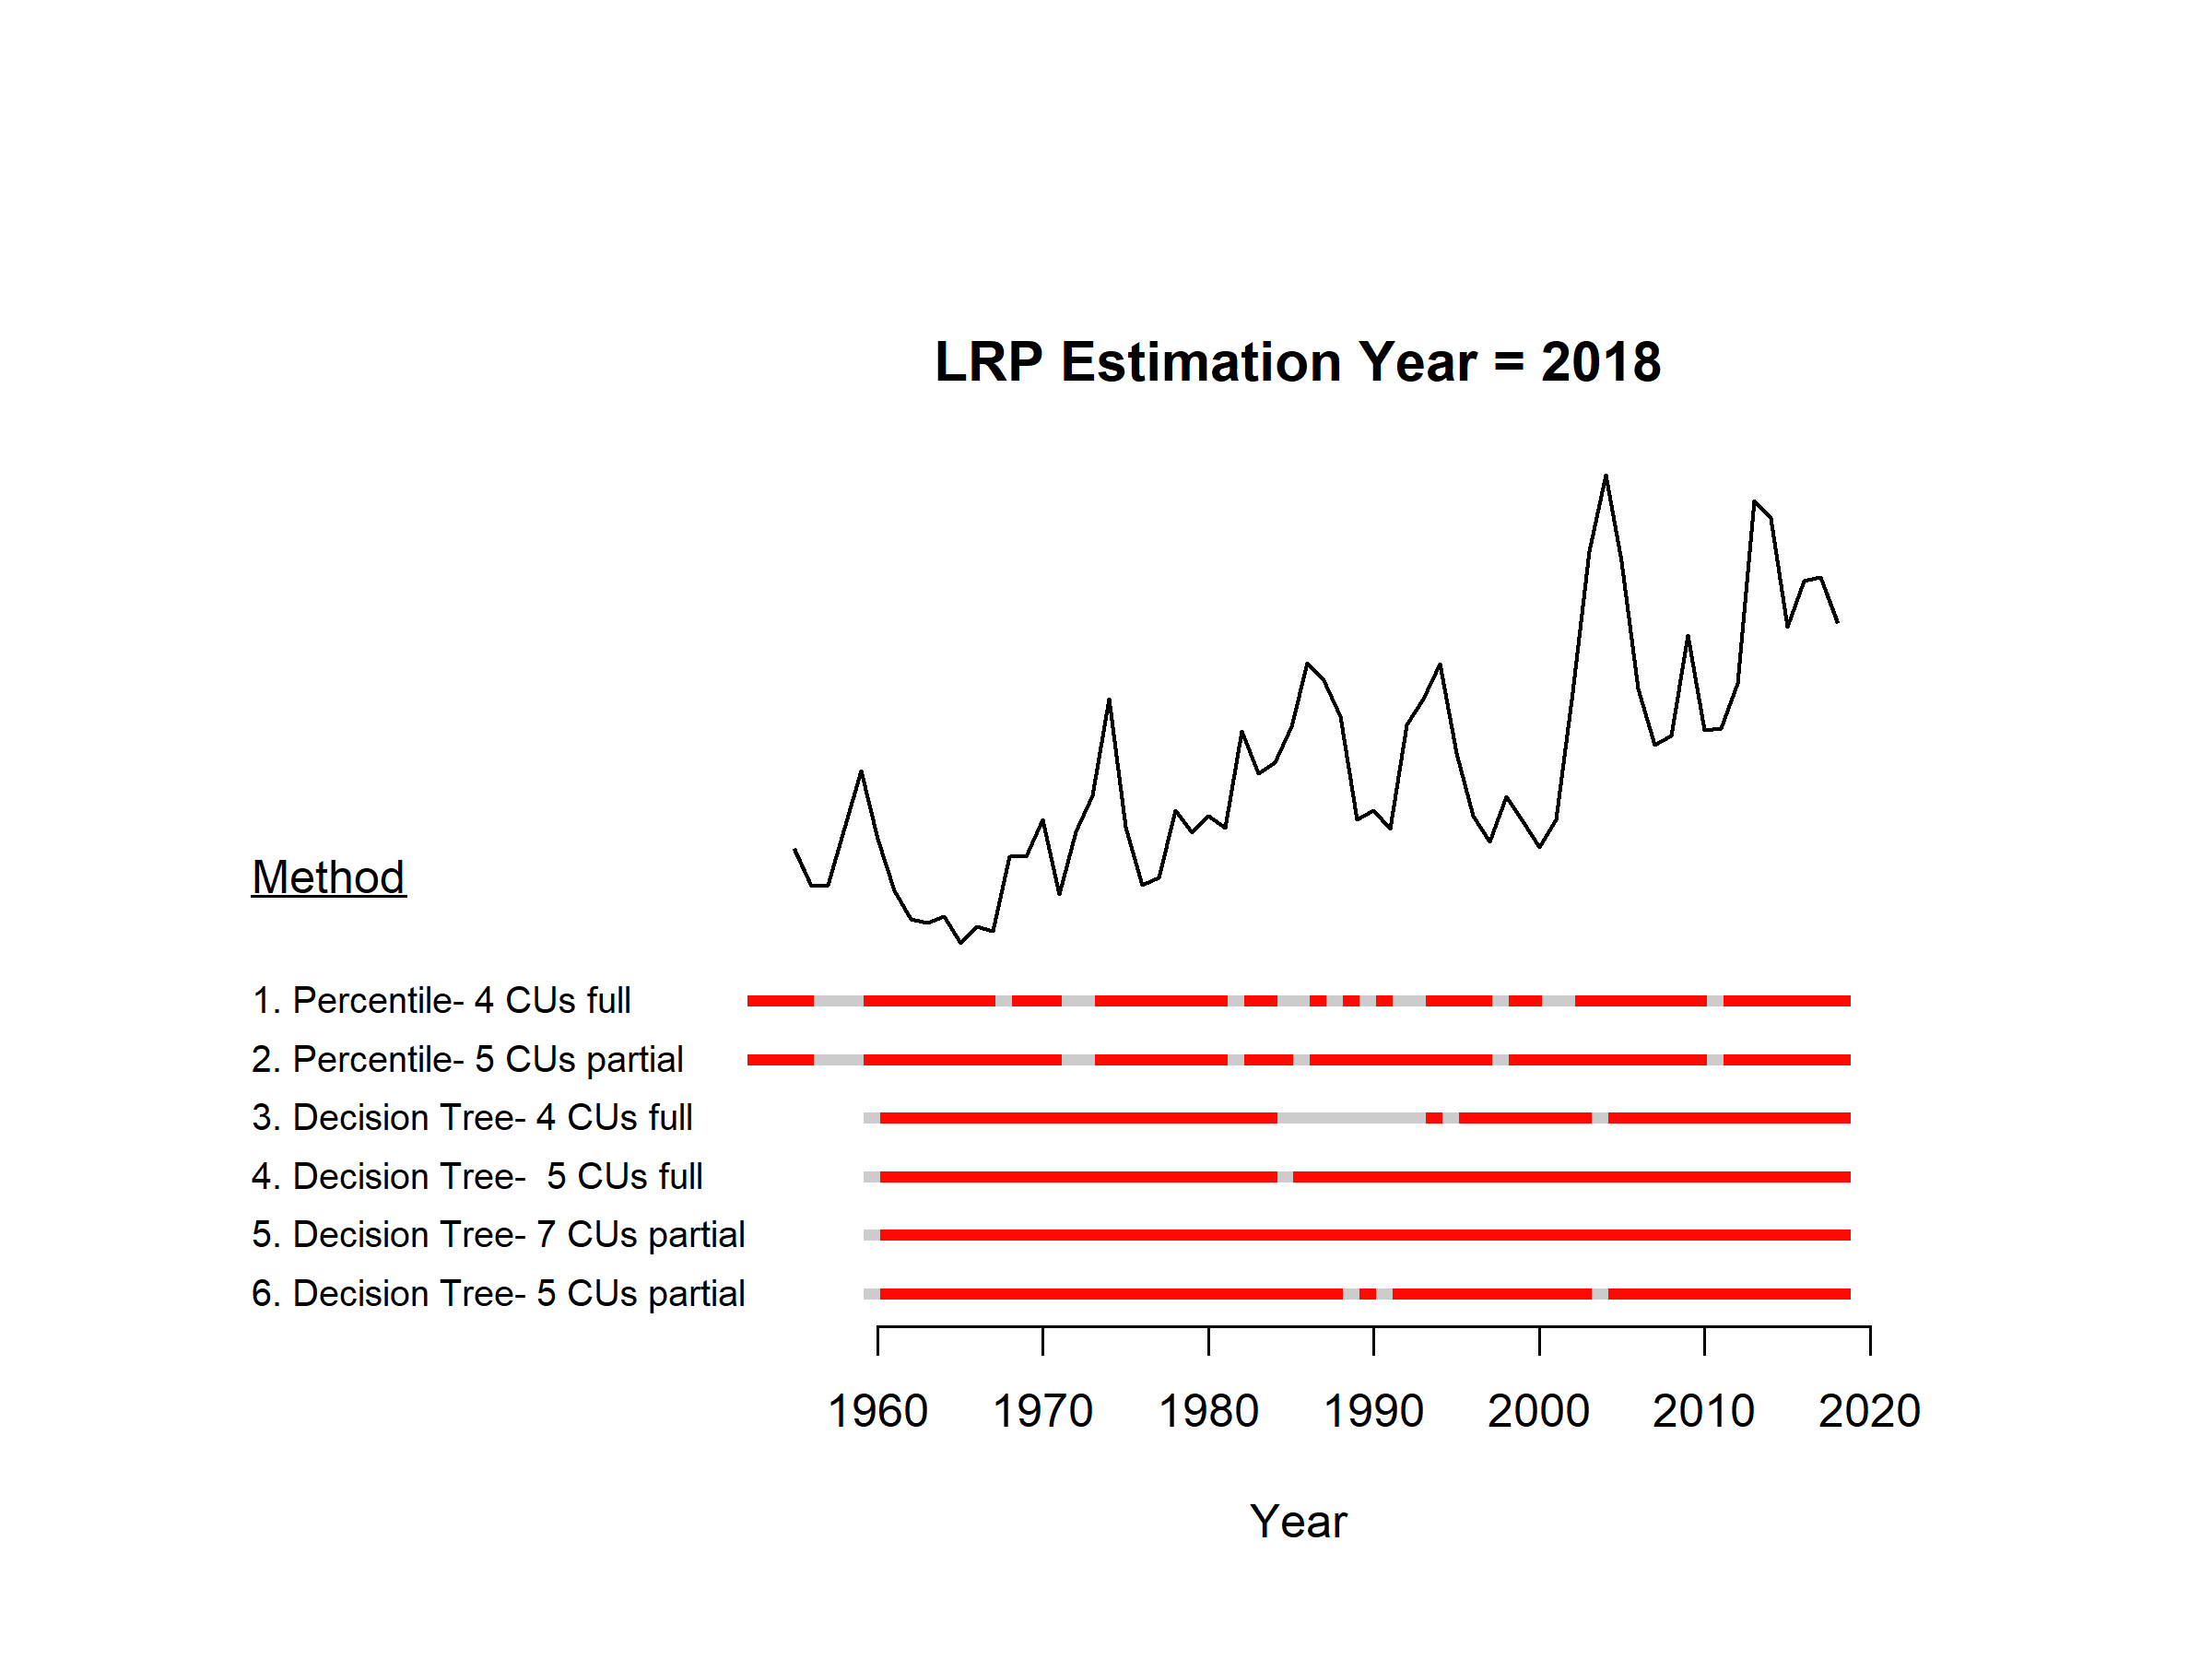
\includegraphics[width=6in]{figure/chum-compare-LRP-methods}}{Figure \ref{fig:chum-LRP-compare}} 

}

\caption{Comparison of LRP status (red = below LRP, gray = above LRP) for six scenarios. The black line shows aggregate abundance. Scenarios 1-3 and 6 do not include Bute Inlet or Southern Coastal Streams (no appropriate percentile benchmarks). 'Full' scenarios use only years with full time series (no CU-level infilled CUs) and 'partial' scenarios include CU-level infilled CUs but drop years with CU-level infilling for those CUs.}\label{fig:chum-LRP-compare}
\end{figure}
\hypertarget{discussion-1}{%
\subsection{Discussion}\label{discussion-1}}

-----------------------edit below here

\hypertarget{lrps-based-on-logistic-regression-and-smu-aggregate-abundance}{%
\subsubsection{LRPs Based on Logistic Regression and SMU Aggregate Abundance}\label{lrps-based-on-logistic-regression-and-smu-aggregate-abundance}}

\hypertarget{discussion-2}{%
\subsection{DISCUSSION}\label{discussion-2}}

\hypertarget{suitability-of-lrp-based-on-status-of-component-cus-proportion}{%
\subsubsection{Suitability of LRP based on status of component CUs (proportion)}\label{suitability-of-lrp-based-on-status-of-component-cus-proportion}}

Something about portfolio effects/ theory. Paper on Alaska shifting productivity areas from year to year.

(Note: not using percentile benchmarks for relative abundance benchmark for decision tree gives the same results as scenario 5 at the SMU level)

\textbf{Limitations of Percentile Benchmarks}

There are some assumptions and limitations when using benchmarks based on percentiles of abundance. One of the largest is the influence of shifting baselines on percentile benchmarks. If abundance has decreased over time, the resulting percentile benchmark will also decrease over time as more data is included (Figure~\ref{fig:chum-perc-retro}). This means that the benchmark shifts downward, reinforcing a shifting baseline. A population size that used to be below the benchmark can become above the benchmark, as the benchmark decreases. This can arise from a decrease in abundance in the period of data, and by an unrecorded high level of abundance before the period of data followed by a decrease before data are available.

The concept of percentile benchmarks also assumes productivity is stationary. Otherwise, if productivity was decreasing, a larger abundance of spawners would be required to produce the same number of recruits. Contrary to this assumption, there is evidence that the productivity of chum salmon is not stationary. The productivity of BC chum salmon is lower when the abundance of North American salmon like pink, sockeye, and chum is greater (\protect\hyperlink{ref-debertinMarineGrowthPatterns2017}{Debertin et al.} (\protect\hyperlink{ref-debertinMarineGrowthPatterns2017}{2017}), \protect\hyperlink{ref-litzCompetitionOddyearPink2021}{Litz et al.} (\protect\hyperlink{ref-litzCompetitionOddyearPink2021}{2021})). The percentile benchmark is also only informed by the data available, which may be for a short time period. Those using percentile benchmarks should also consider whether they are calculated using a percentile of recruits or escapement.

Estimating relative-abundance benchmarks for salmon populations without a long time series and without data on productivity (only escapement, no recruits/smolt production) is challenging. Previous evaluations of Inside South Coast chum population status used a 25\% benchmark (\protect\hyperlink{ref-hilbornBritishColumbiaChum2012}{Hilborn et al.} (\protect\hyperlink{ref-hilbornBritishColumbiaChum2012}{2012})). This was based on previous work by the Alaska Department of Fish and Game that defined four tiers of populations based on contrast in spawner abundances, harvest rate, and precision of escapement data (\protect\hyperlink{ref-bueEscapementGoalReview2001}{Bue and Hasbrouck} (\protect\hyperlink{ref-bueEscapementGoalReview2001}{2001}), \protect\hyperlink{ref-otisEscapementGoalsSalmon2004}{Otis and Hasbrouck} (\protect\hyperlink{ref-otisEscapementGoalsSalmon2004}{2004})). The goal of these tiers was to choose a Sustainable Escapement Goal (an upper and lower percentile) to use as a goal for escapement to represent a proxy for keeping escapement within a range that includes \(S_{MSY}\) (\protect\hyperlink{ref-clarkEvaluationPercentileApproach2014}{Clark et al.} (\protect\hyperlink{ref-clarkEvaluationPercentileApproach2014}{2014})). These SEGs were calculated for each major river/system and are still done that way in Alaska (\protect\hyperlink{ref-mckinleyReviewSalmonEscapement2020}{McKinley et al.} (\protect\hyperlink{ref-mckinleyReviewSalmonEscapement2020}{2020})). Tier 1 of this method was for high escapement contrast (greater than 8 ) and at least moderate harvest rate, with a SEG of 25th to 75th percentiles. \protect\hyperlink{ref-bueEscapementGoalReview2001}{Bue and Hasbrouck} (\protect\hyperlink{ref-bueEscapementGoalReview2001}{2001}) assessed this method on 11 populations of sockeye salmon and Chinook salmon from Upper Cook Inlet and Bristol Bay (in \protect\hyperlink{ref-clarkEvaluationPercentileApproach2014}{Clark et al.} (\protect\hyperlink{ref-clarkEvaluationPercentileApproach2014}{2014}) ). \protect\hyperlink{ref-clarkEvaluationPercentileApproach2014}{Clark et al.} (\protect\hyperlink{ref-clarkEvaluationPercentileApproach2014}{2014}) tested the suitability of this 4 tier percentile approach with theoretical, simulation, and meta-analysis methods using 76 stock-recruitment data sets from Alaska (7 pink salmon, 7 coho salmon, 43 sockeye salmon, 6 chum salmon, and 13 Chinook salmon populations ). They recommended a revised 3 tier system, which changed the Tier 1 lower percentile to 20\%. Moving to British Columbia, \protect\hyperlink{ref-hilbornBritishColumbiaChum2012}{Hilborn et al.} (\protect\hyperlink{ref-hilbornBritishColumbiaChum2012}{2012}) adopted the previous 25\% lower limit of SEG as a benchmark for evaluating the status of Inside South Coast Chum in BC for the purpose of certification with the Marine Stewardship Council (\protect\hyperlink{ref-hilbornBritishColumbiaChum2012}{Hilborn et al.} (\protect\hyperlink{ref-hilbornBritishColumbiaChum2012}{2012})), despite its lack of testing for populations of chum salmon in British Columbia. Further, SEGs were and still are applied to individual rivers in Alaska, compared to the application of this method to entire CUs by \protect\hyperlink{ref-hilbornBritishColumbiaChum2012}{Hilborn et al.} (\protect\hyperlink{ref-hilbornBritishColumbiaChum2012}{2012}), (\protect\hyperlink{ref-holtEvaluatingBenchmarksBiological2018}{\textbf{holtEvaluatingBenchmarksBiological2018?}}), and this study. ISC chum includes 296 streams among the seven CUs, with 126 in Strait of Georgia alone. By aggregating spawners and recruits across many rivers before estimating benchmarks of percentile or stock-recruit parameters, the following problems may arise:
\begin{itemize}

\item
  Error in fitting stock-recruit curves because it is at aggregate level instead of by river
\item
  Sum of \(S_{gen}\) calculated for individual rivers may not equal \(S_{gen}\) calculated using aggregated spawner and recruit data
\item
  Non-stationarity of productivity in individual systems may be hidden by aggregating spawners and recruits
\item
  Spawner abundance at CU level may not be a good predictor of status of individual rivers compared to SEGs at the river scale, depending on the contrast in size between rivers and the correlation (or lack thereof) in escapement and/or productivity
\end{itemize}
\textbf{Salmon Scanner}

Useful for mixture of data qualities/types/BM e.g., some CUs didn't have appropriate RelAbdundance benchmarks. This approach has been tested on a variety of data types, including those with and without relative abundance benchmarks. Like any approach to assess LRP's, the underlying data, and benchmarks applied if relative abundance benchmarks can be used should be verified by experts. There are examples in Fraser Sockeye or with Fraser IFC, where it relied on trend metrics only, so can relate to data types that are data limited for Chum.

\hypertarget{suitability-of-logistic-regression-lrps-based-on-aggregate-abundance}{%
\subsubsection{Suitability of Logistic Regression LRPs Based on Aggregate Abundance}\label{suitability-of-logistic-regression-lrps-based-on-aggregate-abundance}}

Did not work for ISC Chum SMU.

Data was not suited to logistic regression - aggregate abundance was not a good predictor of the status of component CUs.

Some reasons why (summarise from Results): - large differences in abundnace between CUs - 2 orders of magnitude gor Goergia Strait, Howe Sound-Burrard Inlet compared to others. Not high correlation between escapements between CUs. -

Why (further) ? - Large geographical range of SMU / component CUs - Lots of different populations - CUs have different numbers of populations (big differences), and those populations have big differences in abundance - Differences in productivity among CUs/populations

In the retrospective analysis, the logistic model fits were more appropriate to the data in some years (e.g., 1980s). Although logistic regression could be used to estimated LRPs based on aggregate abundance in some SMUs where abundance is more even among CUs and escapements are more correlated, these relationships may not remain static and could become unreasonable over time. Care should be taken to regularly reassess the validity of aggregate abundance-based LRPs where they are implemented in the future.

\hypertarget{assumptions-and-limitations}{%
\subsubsection{Assumptions and limitations}\label{assumptions-and-limitations}}

The CUs that required CU-level infilling (Upper Knight and Bute Inlet) were not used for the retrospective analysis because the assumption that escapement is correlated between CUs ignores diversity between CUs and the potential for uncorrelated escapements. The reality of uncorrelated escapements must be taken into account to evaluate whether aggregate escapement is a meaningful predictor for the status of individual CUs. It should also be noted that these two CUs do not represent a random subset of the seven CUs in the Inside South Coast Chum SMU.

There are studies showing that a range of factors may affect the productivity of ISC Chum. These include competition with other salmon in the ocean and ocean conditions (\protect\hyperlink{ref-debertinMarineGrowthPatterns2017}{Debertin et al.} (\protect\hyperlink{ref-debertinMarineGrowthPatterns2017}{2017}), \protect\hyperlink{ref-litzCompetitionOddyearPink2021}{Litz et al.} (\protect\hyperlink{ref-litzCompetitionOddyearPink2021}{2021})). This application of percentile benchmarks does not account for changing productivity.

\hypertarget{other-sources-of-information-to-inform-lrps-benchmarks}{%
\subsubsection{Other sources of information to inform LRPs / benchmarks}\label{other-sources-of-information-to-inform-lrps-benchmarks}}

Indigenous Knowledge
\begin{itemize}

\item
  Two-Eyed Seeing - Etuaptmumk(Mi'kmaw) \protect\hyperlink{ref-reidTwoEyedSeeingIndigenous2020}{Reid et al.} (\protect\hyperlink{ref-reidTwoEyedSeeingIndigenous2020}{2020})
\item
  Historical baseline before records from western science \protect\hyperlink{ref-eckertDivingBackTime2018}{Eckert et al.} (\protect\hyperlink{ref-eckertDivingBackTime2018}{2018}), \protect\hyperlink{ref-leeDiverseKnowledgeSystems2019}{Lee et al.} (\protect\hyperlink{ref-leeDiverseKnowledgeSystems2019}{2019}), \protect\hyperlink{ref-banIncorporateIndigenousPerspectives2018}{Ban et al.} (\protect\hyperlink{ref-banIncorporateIndigenousPerspectives2018}{2018})
\end{itemize}
Genetic tools and historical records
\begin{itemize}

\item
  Skeena sockeye \protect\hyperlink{ref-priceGeneticsCenturyOld2019}{Price et al.} (\protect\hyperlink{ref-priceGeneticsCenturyOld2019}{2019}), \protect\hyperlink{ref-pricePortfolioSimplificationArising2021}{Price et al.} (\protect\hyperlink{ref-pricePortfolioSimplificationArising2021}{2021})
\item
  Skeena chum \protect\hyperlink{ref-priceAbundanceSkeenaRiver2013}{Price et al.} (\protect\hyperlink{ref-priceAbundanceSkeenaRiver2013}{2013})
\item
  Cannery records (\protect\hyperlink{ref-meengs_estimating_2005}{\textbf{meengs\_estimating\_2005?}})
\end{itemize}
Archaeological records
\begin{itemize}

\item
  BC herring \protect\hyperlink{ref-mckechnieArchaeologicalDataProvide2014}{McKechnie et al.} (\protect\hyperlink{ref-mckechnieArchaeologicalDataProvide2014}{2014})
\end{itemize}
\hypertarget{lessons-learned-from-case-study-applications}{%
\section{LESSONS LEARNED FROM CASE STUDY APPLICATIONS}\label{lessons-learned-from-case-study-applications}}

To be completed.
\begin{itemize}

\item
  Synthesize main results and conclusions from case studies
\end{itemize}
\hypertarget{cu-level-benchmarks-and-assessments}{%
\subsection{CU-level benchmarks and assessments}\label{cu-level-benchmarks-and-assessments}}

LRPs described in this working paper rely on CU-level benchmarks and assessments, for which data vary in quality and quantity. Our case studies demonstrate the application of proportion-based and aggregate-abundance based LRPs to SMUs containing CUs with a range of data availability including those with stock-recruitment benchmarks, habitat-based benchmarks, and spawner abundances percentile-based benchmarks. In addition, we demonstrate assessments for SMUs containing CUs without abundance-based benchmarks where statuses rely on short and long-term trends over time, as demonstrated in application of the Rapid Multidimensional Scanner Tool to Inside Southcoast Chum - Non Fraser.

At the CU-level, we found that using a single metric, spawner abundances relative to a WSP lower benchmark (\(S_{gen}\) or percentiles) resulted in similar status assessments to using the Rapid Multidimensional Scanning Tool. These similarities occur because when the lower benchmarks estimates are available, the rapid multidimensional scanning tool will almost always default to assessing status against them, as was demonstrated for all three case studies. Exceptions occur when the lower benchmark estimates are below the absolute population thresholds (e.g., below 1500 spawners) and available spawner time-series are absolute numbers, as occurred for the Interior Fraser Coho study case for 1 CU in 3 years. In these cases, the Rapid Multidimensional Scanning Tool triggered red status due to low abundances below the absolute conservation threshold even though the stock-recruitment based lower benchmark was not breached.

In addition, we found that using the Rapid Multidimensional Scanning Tool allows for the consideration of CUs that would otherwise be considered data deficient using single metric on spawner abundances relative to benchmarks, thus allowing for a more complete assessment of the SMU status. In these cases, the Rapid Multidimensional Scanning Tool is able to provide an assessment of status based on short and long-term trends when benchmarks on spawner abundances are not available, as demonstrated in the Inside South Coast Chum case study. The possibility of assessing CUs lacking abundance-based lower benchmarks is particularly important when SMUs are composed of CU with low levels of synchrony in which data deficient CUs cannot be represented by proxy. The status assessment based on trends is also useful when the CUs lacking lower benchmark estimates are small. Representing small CUs by proxy is problematic because the small CUs tend to be more vulnerable than larger CUs even if productivity is similar (cite).

\hypertarget{smu-level-lrps-and-assessments}{%
\subsection{SMU-level LRPs and assessments}\label{smu-level-lrps-and-assessments}}

All of the LRP estimation methods we considered were based on status estimates for component CUs; regardless of whether it was a proportion-based or abundance-based method. As a result, the reliability of LRP estimates is a function of the reliability of individual CU status estimates. The effect of uncertainty in CU-level benchmarks on resulting estimates of LRP status was apparent in the Interior Fraser Coho case study where two different structural assumptions in stock recruitment model fit were considered. These two model fits resulted in different estimates of productivity and carrying capacity for individual CUs, as well as different estimates of Sgen. These two different model formulations resulted in different estimates of SMU status relative to LRPs over time for all LRP estimation methods considered for Interior Fraser Coho.

We found that removing component CUs from assessments impacted the SMU-level status, resulting in SMU assessments that may be more pessimistic or optimistic than when all CUs are considered, depending on the level of covariation among CUs, status of other component CUs and, CU sizes. There is, however, and asymmetry in how missing CUs may affect the SMU status. If the LRP of 100\% of CUs above red status has been breached for an SMU, the inclusion of additional CUs may further deplete or improve status (\% of CUs above red), but will not increase status to above the LRP (100\%). In contrast, if the LRP is not breached for an SMU, then the inclusion of additional CUs may deplete status to below the LRP or keep status at 100\% of CUs above red zone. This asymmetrical impact of increased monitoring of CUs on SMU status may reduce incentives to extend monitoring to data-deficient CUs.

For SMUs with component CUs that vary independently of each other, the inclusion of additional CU-level assessments will increase the likelihood of the proportion-based LRP being breached. For example, for the Inside South Coast Chum case study, when data-limited CUs were included in the derivation of proportion-based LRPs (i.e., CUs without percentile-based benchmarks), the proportion-based LRP was breached more often in historical analyses compared to when those CUs were excluded. For this case study, the exclusion of CUs with incomplete time series led to overoptimistic assessments in some years compared to when those CUs were included. Our results from this case study highlight the importance of including data from all CUs when CUs show high variability in status estimates. Guidelines on identifying where data-rich CUs are more likely to provide status that is representative of data-deficient CUs and hence can be omitted from SMU-level LRPs and assessments is provided in Holt et al.~(in review).

For both proportion-based and aggregate-abundance based LRPs, we found that status assessments were sensitive to assumptions about the structural form of the underlying spawner-recruitment model used to estimate the lower benchmark, \(S_{gen}\), and to considerations of different types of lower benchmarks, e.g., those reflecting distribution of spawners as considered in the Interior Fraser River Coho case study. The decision on which structural form or type of benchmarks to consider depends on the biological characteristics of the populations and available data, highlighting the importance of considering expert knowledge and peer-reviewed WSP assessments for determining CU status. This challenge of identifying the most appropriate model form is pervasive across fisheries stock assessments and brings risks of basing assessments on incorrect or incomplete model forms. In our case studies we identify several approaches for addressing this challenge, such as implementing sensitivity analyses to various assumptions and ensemble modeling where outputs from various assumptions are combined in a probabilistic way.

\hypertarget{logistic-regression-based-lrps}{%
\subsubsection{Logistic regression-based LRPs}\label{logistic-regression-based-lrps}}

Logistic regression-based LRPs are empirically derived from the past observations of SMU abundance and CU statuses. By fitting a logistic regression to these historical data, we identify historical abundance levels associated with probabilities that all component CUs have statuses above their lower benchmarks. Similarly to the proportion-based LRP, this aggregate abundance method depends on the outcomes of individual CU assessments, which are sensitive to structural assumptions underlying the CU-level benchmarks and data availability. Logistic regression-based LRPs could only be estimated for one of our three case study SMUs, which suggests that they may only be an option for a small proportion of SMUs. Logistic regression models could not be reliably fit for WCVI Chinook and South Coast Chum SMUs. In the case of WCVI Chinook, lack of contrast in available data was the key limitation, while in the case of South Coast Chum, the limitation was an apparent lack of an underlying relationship between CU status and aggregate SMU abundances. Even for Interior Fraser Coho where a logistic regression fit was possible, estimates did not converge for all retrospective years, and status estimates were sensitive to missing data. Taken together, our exploration of logistic regression LRPs for our three case studies highlighted several key limitations and disadvantages with this approach.

There are several disadvantages of the logistic regression-based LRPs. First, our implementation of logistic-regression LRPs relied on a single metric for CU assessments, such as \(S_{gen}\) or the distributional target method applied to the Interior Fraser Coho study case study, which is not consistent with the recommendation to to apply the Rapid Multidimensional Scanner tool for CU assessments within proportion-based LRPs. We did not include CU assessments based on the multidimensional approach for logistic-regression based LRPs in part because those statuses include trend metrics which introduce autocorrelation into CU statuses, a violation of logistic regression model (see Section 2 for more details).

Second, logistic regression-based LRPs are only estimable when there are years when all CUs or sub-populations are above their lower benchmark and years when at least one CU is below their lower benchmarks. This was not the case for the WCVI Chinook study case due to one inlet always been below its lower benchmark.

Third, model diagnostics do not support logistic regressions and their associated LRPs when CU-level abundances are not correlated or only weakly correlated. For these SMUs, the aggregate abundances are not a significant indicator of individual CU statuses. Here, we found that logistic regression-based LRPs were estimable for interior Fraser Coho (average correlation within CUS of 0.43) but not estimable for Inside South Coast Chum - Non-Fraser (average correlation within CUs of XX). Also, the wide rand in productivities and capacities among CUs for the Inside South Coast Chum case study contributed to the weak relationship between aggregate abundances and CU-level statuses. In general, model diagnostics as described in~\ref{MethodsChapters} can be used to support or reject logistic-regression based LRPs.

Missing data for individual CUs within an SMU may also pose a problem for the estimation of logistic regression-based LRPs. When data are missing for one or more CUs within and SMU, it may still be appropriate to apply the logistic regression-based LRP to the remaining CUs with data to assess status for the entire SMU. This is particularly true if there are high levels of covariation between the CUs. However, the logistic regression model fit will degenerate as the number of CUs with missing data increases. Sensitivity analysis for the Interior Fraser Coho study case showed that the model fit degenerated when two CU data sets were removed from the analysis. The influence of missing data was also dependent on the status of the CU for which data was missing. The omission of a CU with red status will be more influential that omitting data for a CU with amber or green status because the red status would trigger the LRP and change the SMU status for the logistic regression, biasing the aggregate abundance LRP to lower values.

Finally, it is important to inspect model diagnostics and statistically test the model assumptions whenever applying the logistic regression-based LRPs. In chapter~\ref{lrp-estimation-methods} we provide a list of model diagnostics that should be checked when applying this aggregate abundance LRP estimation method. In addition, we illustrate how the diagnostics are used in support of the model fit in chapter~\ref{IFCChapter}, and against the model fit in the~\ref{ISCchumChapter}.

\hypertarget{projection-based-lrps}{%
\subsubsection{Projection based LRPs}\label{projection-based-lrps}}

The projection-based LRPs approach relies on closed-loop simulation models to project future CU abundances. These projections are then used to quantify the relationship between aggregate SMU abundances and the probabilities that all CUs are above their lower benchmarks, given a predefined level of exploitation. The most important requirement for our implementation of projection-based LRPs is the availability of information on productivity and capacity for the CUs within an SMU, and covariance in dynamics among them. Parameter estimates for productivity and capacity can be based on posterior distributions from stock recruitment analyses (see Interior Fraser Coho study case, chapter~\ref{IFCChapter}) or more qualitatively from expert input, life-stage models, or watershed-area model estimates (see WCVI Chinook study case, chapter~\ref{WCVIchinookChapter}).

The projection-based LRP approach is flexible and allows for consideration of structural uncertainty in the SMU population dynamics via consideration of alternative future scenarios. For example, for the WCVI Chinook case study, sensitivity analyses were performed to assess the impacts of correlations in recruitment residuals and variability in exploitation among inlets. For the Interior Fraser Coho study case, sensitivity analyses were performed regarding the variability in marine survival coefficient among CUs. Future implementations of the projection-based LRPs could also take into consideration shifts in stock recruitment parameters, and future changes in fishery exploitation rates.

We also demonstrated that projection-based LRPs are sensitive to the assumed levels of exploitation in the projections. Higher exploitation rates resulted in higher required SMU aggregate abundance to ensure that all CUs remain above their lower benchmarks. The sensitivity to exploitation rate increases as variability in stock-recruitment parameters among CUs increase, and also as uncertainty in parameter estimates increase. This property of projection-based LRPs is explored in Appendix~\ref{app:ERsensitivity-appendix}. Therefore projection-based LRPs developed under historical and current exploitation rates cannot necessarily be used as a basis for evaluating alternative management procedures. However demonstrating the changes in aggregate abundances required for all CUs to be above lower benchmarks (i.e.~changes in projection-based LRP) under different exploitation scenarios may help analysts and managers understand the implications of changing exploitation rates on the ability to achieve WSP objectives.

\clearpage

\hypertarget{references}{%
\section{REFERENCES}\label{references}}

% This manually sets the header for this unnumbered chapter.
\noindent
\vspace{-2em}
\setlength{\parindent}{-0.2in}
\setlength{\leftskip}{0.2in}
\setlength{\parskip}{8pt}

\hypertarget{refs}{}
\begin{CSLReferences}{1}{0}
\leavevmode{\hypertarget{ref-ahmadDiagnosticResidualOutliers2011}{}}%
Ahmad, S. 2011. Diagnostic for residual outliers using deviance component in binary logistic regression. World Applied Sciences Journal 14(8): 1125--1130.

\leavevmode{\hypertarget{ref-arbeiderInteriorFraserCoho2020}{}}%
Arbeider, M., Ritchie, L., Braun, D., Jenewein, B., Rickards, K., Dionne, K., Holt, C., Labelle, M., Nicklin, P., Mozin, P., Grant, P., Parken, C., and Bailey, R. 2020. Interior {Fraser} {Coho} {Salmon} {Recovery} {Potential} {Assessment}. Canadian Science Advisory Secretariat Research Document 2020/025: xi + 222p.

\leavevmode{\hypertarget{ref-banIncorporateIndigenousPerspectives2018}{}}%
Ban, N.C., Frid, A., Reid, M., Edgar, B., Shaw, D., and Siwallace, P. 2018. Incorporate {Indigenous} perspectives for impactful research and effective management. Nature Ecology \& Evolution 2(11): 1680--1683.

\leavevmode{\hypertarget{ref-brown2020SummaryAbundance2020}{}}%
Brown, G.S., Thiess, M.E., Wor, C., Holt, C.A., Patten, B., Bailey, R.E., Parken, C.K., Baillie, S.J., Candy, J.R., Willis, D.M., Hertz, E., Connors, B., and Pestal, G.P. 2020. 2020 {Summary} of {Abundance} {Data} for {Chinook} {Salmon} (\emph{{Oncorhynchus} tshawytscha}) in {Southern} {British} {Columbia}, {Canada}.

\leavevmode{\hypertarget{ref-bueEscapementGoalReview2001}{}}%
Bue, B.G., and Hasbrouck, J.J. 2001. Escapement goal review of salmon stocks of {Upper} {Cook} {Inlet}. Report to the \{Board\} of \{Fisheries\} \{November\} 2001, Alaska Department of Fish; Game, Anchorage.

\leavevmode{\hypertarget{ref-dfoCanadaPolicyConservation2005}{}}%
Canada's {Policy} for {Conservation} of {Wild} {Pacific} {Salmon}. 2005. Fisheries; Oceans Canada, Vancouver.

\leavevmode{\hypertarget{ref-clarkEvaluationPercentileApproach2014}{}}%
Clark, R.A., Eggers, D.M., Munro, A.R., Fleischman, S.J., Bue, B.G., and Hasbrouck, J.J. 2014. An {Evaluation} of the {Percentile} {Approach} for {Establishing} {Sustainable} {Escapement} {Goals} in {Lieu} of {Stock} {Productivity} {Information}. Alaska Department of Fish; Game.

\leavevmode{\hypertarget{ref-cosewicCOSEWICAssessmentStatus2016}{}}%
COSEWIC. 2016. {COSEWIC} assessment and status report on the {Coho} {Salmon} (\emph{{Oncorhynchus} kisutch}), {Interior} {Fraser} population, in {Canada}. Committee on the Status of Endangered Wildlife in Canada. Ottawa: xi + 50 p.

\leavevmode{\hypertarget{ref-coxCandidateLimitReference2019}{}}%
Cox, S.P., Benson, A.J., Cleary, J.S., and Taylor, N.G. 2019. Candidate {Limit} {Reference} {Points} as a {Basis} for {Choosing} {Among} {Alternative} {Harvest} {Control} {Rules} for {Pacific} {Herring} ({Clupea} pallasii) in {British} {Columbia}. Canadian Science Advisory Secretariat Research Document 2019/050: viii + 47 p.

\leavevmode{\hypertarget{ref-debertinMarineGrowthPatterns2017}{}}%
Debertin, A.J., Irvine, J.R., Holt, C.A., Oka, G., and Trudel, M. 2017. Marine growth patterns of southern {British} {Columbia} chum salmon explained by interactions between density-dependent competition and changing climate. Canadian Journal of Fisheries and Aquatic Sciences 74(7): 1077--1087.

\leavevmode{\hypertarget{ref-deckerAssessmentInteriorFraser2014}{}}%
Decker, A.S., Hawkshaw, M.A., Patten, B.A., Sawada, J., and Jantz, A.L. 2014. Assessment of the {Interior} {Fraser} {Coho} {Salmon} (\emph{{Oncorhynchus} kisutch}) {Management} {Unit} {Relative} to the 2006 {Conservation} {Strategy} {Recovery} {Objectives}. Canadian Science Advisory Secretariat Research Document 2014/086: xi + 64 p.

\leavevmode{\hypertarget{ref-dfoAssessmentWestCoast2012}{}}%
DFO. 2012. Assessment of {West} {Coast} {Vancouver} {Island} {Chinook} and 2010 forecast. \{DFO\} \{Can\}. \{Sci\}. \{Advis\}. \{Sec\}. \{Sci\}. \{Advis\}. \{Rep\}.

\leavevmode{\hypertarget{ref-dfoWildSalmonPolicy2015}{}}%
DFO. 2015. Wild salmon policy biological status assessment for conservation units of interior {Fraser} {River} {Coho} {Salmon} (\emph{{Oncorhynchus} kisutch}). DFO Canadian Science Advisory Secretariat Science Advisory Report 2015/022: 12.

\leavevmode{\hypertarget{ref-dfoIntegratedBiologicalStatus2016}{}}%
DFO. 2016. Integrated {Biological} {Status} of {Southern} {British} {Columbia} {Chinook} {Salmon} (\emph{{Oncorhynchus} tshawytscha}) under the {Wild} {Salmon} {Policy}. \{DFO\} \{Can\}. \{Sci\}. \{Advis\}. \{Sec\}. \{Sci\}. \{Advis\}. \{Rep\}.

\leavevmode{\hypertarget{ref-dfo2017FraserSockeye2018}{}}%
DFO. 2018. The 2017 {Fraser} {Sockeye} {Salmon} (\emph{{Oncorhynchus} nerka}) integrated biological status re-assessment under the {Wild} {Salmon} {Policy}. \{DFO\} \{Can\}. \{Sci\}. \{Advis\}. \{Sec\}. \{Sci\}. \{Advis\}. \{Rep\}.

\leavevmode{\hypertarget{ref-dfoIntegratedFisheriesManagement2021}{}}%
DFO. 2021a. Integrated {Fisheries} {Management} {Plan} {June} 1, 2021 - {May} 31, 2022, {Salmon} {Southern} {BC}.

\leavevmode{\hypertarget{ref-dfoWCVISalmonBulletin2021}{}}%
DFO. 2021b. {WCVI} {Salmon} {Bulletin} 2021, {WCVI} {Chinook} {Terminal} {Forecast}.

\leavevmode{\hypertarget{ref-dobsonIntroductionGeneralizedLinear2018}{}}%
Dobson, A., and Barnett, A.G. 2018. An introduction to generalized linear models. CRC press.

\leavevmode{\hypertarget{ref-eckertDivingBackTime2018}{}}%
Eckert, L.E., Ban, N.C., Frid, A., and McGreer, M. 2018. Diving back in time: {Extending} historical baselines for yelloweye rockfish with {Indigenous} knowledge. Aquatic Conservation: Marine and Freshwater Ecosystems 28(1): 158--166.

\leavevmode{\hypertarget{ref-forrestAssessmentPacificCod2020}{}}%
Forrest, R.E., Anderson, S.C., Gr, in, J., C., and Starr, P.J. 2020. Assessment of {Pacific} {Cod} ({Gadus} macrocephalus) for {Hecate} {Strait} and {Queen} {Charlotte} {Sound} ({Area} {5ABCD}), and {West} {Coast} {Vancouver} {Island} ({Area} {3CD}) in 2018. Canadian Science Advisory Secretariat Research Document 2020/070: v + 215 p.

\leavevmode{\hypertarget{ref-foxAppliedRegressionAnalysis2016}{}}%
Fox, J. 2016. Applied {Regression} {Analysis} and {Generalized} {Linear} {Models}. \emph{In} Third. Sage Publications Inc.

\leavevmode{\hypertarget{ref-frameGuidanceNoteLead2010}{}}%
Frame, D.J., Held, H., Kriegler, E., Mach, K.J., Matschoss, P.R., Plattner, G.-K., Zwiers, F.W., and Matschoss, P.R. 2010. Guidance {Note} for {Lead} {Authors} of the {IPCC} {Fifth} {Assessment} {Report} on {Consistent} {Treatment} of {Uncertainties}.~: 7.

\leavevmode{\hypertarget{ref-freshwaterBenefitsLimitationsIncreasing2020}{}}%
Freshwater, C., Holt, K.R., Huang, A.-M., and Holt, C.A. 2020. Benefits and limitations of increasing the stock-selectivity of {Pacific} salmon fisheries. Fisheries Research 226: 105509.

\leavevmode{\hypertarget{ref-governmentofcanadaFisheryDecisionmakingFramework2009}{}}%
Government of Canada, F. and O.C. 2009, March. A fishery decision-making framework incorporating the precautionary approach.

\leavevmode{\hypertarget{ref-grant2017FraserSockeye2020}{}}%
Grant, S.C.H., Holt, C.A., Pestal, G., Davis, B.M., and MacDonald, B.L. 2020. The 2017 {Fraser} {Sockeye} {Salmon} ({Oncorhynchus} nerka) {Integrated} {Biological} {Status} {Re}-{Assessments} {Under} the {Wild} {Salmon} {Policy} {Using} {Standardized} {Metrics} and {Expert} {Judgment}.~: 218.

\leavevmode{\hypertarget{ref-hilbornBritishColumbiaChum2012}{}}%
Hilborn, R., Schmidt, D., English, K., and Devitt, S. 2012. British {Columbia} {Chum} {Salmon} (\emph{{Oncorhynchus} keta}) {Fisheries}: {British} {Columbia} {Coastal} and {Adjacent} {Canadian} {Pacific} {EEZ} {Waters}, {Final} {Certification} {Report}. Submitted to Canadian Pacific Sustainable Fisheries Society.

\leavevmode{\hypertarget{ref-holtIndicatorsStatusBenchmarks2009}{}}%
Holt, C.A., Cass, A., Holtby, B., and Riddell, B. 2009. Indicators of {Status} and {Benchmarks} for {Conservation} {Units} in {Canada}'s {Wild} {Salmon} {Policy}.~: 82.

\leavevmode{\hypertarget{ref-holtCautionsUsingPercentilebased2015}{}}%
Holt, C.A., and Folkes, M.J.P. 2015. Cautions on using percentile-based benchmarks of status for data-limited populations of {Pacific} salmon under persistent trends in productivity and uncertain outcomes from harvest management. Fisheries Research 171: 188--200.

\leavevmode{\hypertarget{ref-holtQuantitativeToolEvaluating2020}{}}%
Holt, C.A., Freshwater, C., Holt, K.R., and Huang, A.M. 2020. A quantitative tool for evaluating rebuilding plans for {Pacific} salmon.

\leavevmode{\hypertarget{ref-holtbyConservationUnitsPacific2007}{}}%
Holtby, L.B., and Ciruna, K.A. 2007. Conservation {Units} for {Pacific} {Salmon} under the {Wild} {Salmon} {Policy}. Research \{Document\}, Fisheries; Oceans Canada.

\leavevmode{\hypertarget{ref-ifcrtinteriorfrasercohorecoveryteamConservationStrategyCoho2006}{}}%
IFCRT (Interior Fraser Coho Recovery Team). 2006. Conservation strategy for {Coho} {Salmon} ({Oncorhynchus} kisutch), interior {Fraser} {River} populations. {Fisheries} and {Oceans} {Canada}, {Ottawa}, {Ont}. 132 p.

\leavevmode{\hypertarget{ref-kormanEvaluationFrameworkAssessing2019}{}}%
Korman, J., Sawada, J., and Bradford, M.J. 2019. Evaluation framework for assessing potential {Pacific} {Salmon} {Commission} reference points for population status and associated allowable exploitation rates for {Strait} of {Georgia} and {Fraser} {River} {Coho} {Salmon} {Management} {Units}. Canadian Science Advisory Secretariat Research Document 2019/001: ix + 81 p.

\leavevmode{\hypertarget{ref-kristensenTMBAutomaticDifferentiation2016}{}}%
Kristensen, K., Nielsen, A., Berg, C.W., Skaug, H., and Bell, B.M. 2016. \textbf{TMB}~: {Automatic} {Differentiation} and {Laplace} {Approximation}. Journal of Statistical Software 70(5).

\leavevmode{\hypertarget{ref-leeDiverseKnowledgeSystems2019}{}}%
Lee, L.C., Thorley, J., Watson, J., Reid, M., and Salomon, A.K. 2019. Diverse knowledge systems reveal social--ecological dynamics that inform species conservation status. Conservation Letters 12(2).

\leavevmode{\hypertarget{ref-liermannUsingAccessibleWatershed2010}{}}%
Liermann, M.C., Sharma, R., and Parken, C.K. 2010. Using accessible watershed size to predict management parameters for {Chinook} salmon, (\emph{oncorhynchus} tshawytscha), populations with little or no spawner-recruit data: A {Bayesian} hierarchical modelling approach. Fisheries Management and Ecology 17(1): 40--51.

\leavevmode{\hypertarget{ref-litzCompetitionOddyearPink2021}{}}%
Litz, M., Agha, M., Dufault, A., Claiborne, A., Losee, J., and Anderson, A. 2021. Competition with odd-year pink salmon in the ocean affects natural populations of chum salmon from {Washington}. Marine Ecology Progress Series 663: 179--195.

\leavevmode{\hypertarget{ref-mckechnieArchaeologicalDataProvide2014}{}}%
McKechnie, I., Lepofsky, D., Moss, M.L., Butler, V.L., Orchard, T.J., Coupland, G., Foster, F., Caldwell, M., and Lertzman, K. 2014. Archaeological data provide alternative hypotheses on {Pacific} herring ( \emph{{Clupea} pallasii} ) distribution, abundance, and variability. Proceedings of the National Academy of Sciences 111(9): E807--E816.

\leavevmode{\hypertarget{ref-mckinleyReviewSalmonEscapement2020}{}}%
McKinley, T.R., DeCovich, N., Erickson, J.W., Hamazaki, T., Begich, R., and Vincent, T. 2020. Review of salmon escapement goals in {Upper} {Cook} {Inlet}, {Alaska}, 2019. Alaska Department of Fish; Game, Anchorage.

\leavevmode{\hypertarget{ref-ohlbergerBayesianLifecycleModel2019}{}}%
Ohlberger, J., Brenkman, S.J., Crain, P., Pess, G.R., Duda, J.J., Buehrens, T.W., Quinn, T.P., and Hilborn, R. 2019. A {Bayesian} life-cycle model to estimate escapement at maximum sustained yield in salmon based on limited information. Canadian Journal of Fisheries and Aquatic Sciences 76(2): 299--307.

\leavevmode{\hypertarget{ref-olmosEvidenceSpatialCoherence2019}{}}%
Olmos, M., Massiot‐Granier, F., Prévost, E., Chaput, G., Bradbury, I.R., Nevoux, M., and Rivot, E. 2019. Evidence for spatial coherence in time trends of marine life history traits of {Atlantic} salmon in the {North} {Atlantic}. Fish and Fisheries 20(2): 322--342.

\leavevmode{\hypertarget{ref-otisEscapementGoalsSalmon2004}{}}%
Otis, E.O., and Hasbrouck, J.J. 2004. Escapement goals for salmon stocks in {Lower} {Cook} {Inlet}, {Alaska}. Alaska Department of Fish; Game, Anchorage.

\leavevmode{\hypertarget{ref-parkenHabitatbasedMethodsEstimate2006}{}}%
Parken, C.K., McNicol, R.E., and Irvine, J.R. 2006. Habitat-based methods to estimate escapement goals for data limited {Chinook} salmon stocks in {British} {Columbia}, 2004. \{DFO\} \{Can\}. \{Sci\}. \{Advis\}. \{Sec\}. \{Res\}. \{Doc\}.

\leavevmode{\hypertarget{ref-peduzziSimulationStudyNumber1996}{}}%
Peduzzi, P., Concato, J., Kemper, E., Holford, T.R., and Feinstein, A.R. 1996. A simulation study of the number of events per variable in logistic regression analysis. Journal of Clinical Epidemiology 49(12): 1373--1379.

\leavevmode{\hypertarget{ref-pestalAlgorithmsRapidStatus2021}{}}%
Pestal, G., MacDonald, B., Grant, S., and Holt, C. 2021. Algorithms for {Rapid} {Status} {Approximation} for {Pacific} {Salmon} {Derived} from {Integrated} {Expert} {Assessments} under {Canada}'s {Wild} {Salmon} {Policy}. Canaidan Technical Report of Fisheries and Aquatic Sciences.

\leavevmode{\hypertarget{ref-priceGeneticsCenturyOld2019}{}}%
Price, M.H.H., Connors, B.M., Candy, J.R., McIntosh, B., Beacham, T.D., Moore, J.W., and Reynolds, J.D. 2019. Genetics of century‐old fish scales reveal population patterns of decline. Conservation Letters 12(6).

\leavevmode{\hypertarget{ref-priceAbundanceSkeenaRiver2013}{}}%
Price, M.H.H., Gayeski, N., and Stanford, J.A. 2013. Abundance of {Skeena} {River} {Chum} {Salmon} during the {Early} {Rise} of {Commercial} {Fishing}. Transactions of the American Fisheries Society 142(4): 989--1004.

\leavevmode{\hypertarget{ref-pricePortfolioSimplificationArising2021}{}}%
Price, M.H.H., Moore, J.W., Connors, B.M., Wilson, K.L., and Reynolds, J.D. 2021. Portfolio simplification arising from a century of change in salmon population diversity and artificial production. Journal of Applied Ecology: 1365--2664.13835.

\leavevmode{\hypertarget{ref-reidTwoEyedSeeingIndigenous2020}{}}%
Reid, A.J., Eckert, L.E., Lane, J.-F., Young, N., Hinch, S.G., Darimont, C.T., Cooke, S.J., Ban, N.C., and Marshall, A. 2020. {``{Two}-{Eyed} {Seeing}''}: {An} {Indigenous} framework to transform fisheries research and management. Fish and Fisheries n/a(n/a).

\leavevmode{\hypertarget{ref-riddellReview2001Chinook2002}{}}%
Riddell, B.E., Luedke, W., Till, J., Taylor, S., and Tompkins, A. 2002. Review of 2001 {Chinook} {Returns} to the {West} {Coast} {Vancouver} {Island}, {Forecast} of the 2002 {Return} to the {Stamp} {River} / {Robertson} {Creek} {Hatchery} {Indicator} {Stock}, and {Outlook} for other {WCVI} {Chinook} {Stocks}. Can. Sci. Advis. Sec. Res. Doc. 2006/083. 44.

\leavevmode{\hypertarget{ref-scheuerellExplicitSolutionCalculating2016}{}}%
Scheuerell, M.D. 2016. An explicit solution for calculating optimum spawning stock size from {Ricker}'s stock recruitment model. PeerJ 4: e1623.

\leavevmode{\hypertarget{ref-schnuteInfluenceErrorPopulation1995}{}}%
Schnute, J.T., and Richards, L.J. 1995. The influence of error on population estimates from catch-age models. Canadian Journal of Fisheries and Aquatic Sciences 52(10): 2063--2077.

\leavevmode{\hypertarget{ref-vanwillInnerSouthCoast2014}{}}%
Van Will, P. 2014. Inner {South} {Coast} {Chum} {Stock} {Reconstructions} (1953-2013).

\leavevmode{\hypertarget{ref-withlerGeneticallyBasedTargets2018}{}}%
Withler, R.E., Bradford, M.J., Willis, D.M., and Holt, C.A. 2018. Genetically {Based} {Targets} for {Enhanced} {Contributions} to {Canadian} {Pacific} {Chinook} {Salmon} {Populations}. Research \{Document\}, Fisheries; Oceans Canada.

\end{CSLReferences}
\setlength{\parindent}{0in} \setlength{\leftskip}{0in} \setlength{\parskip}{4pt}

\Appendices


\clearpage

\refstepcounter{chapter}
\label{app:08-appendix-chum-data}
\starredchapter{APPENDIX~\thechapter. Data Sources \& Treatment for Innter South Coast Non-Fraser Chum Salmon}

\hypertarget{spawner-counts-escapement}{%
\appsection{Spawner counts / escapement}\label{spawner-counts-escapement}}

We used spawning escapement data from 1953-2018. Most of the escapement data comes from the NUSEDS database (a small amount from Lower Fraser Stock Assessment for Areas 28 and 29, FSC in-river catch from some First Nations, and enhanced escapement from DFO Salmon Enhancement Program). The number of Chum salmon that return to spawn is typically counted using visual surveys. Biologists from Fisheries and Oceans Canada and First Nations including \ldots{} (Island Marine Aquatic Working Group) \emph{\textcolor{cyan}{LW: which ones?}} generate these data by walking streams and counting fish, \emph{\textcolor{cyan}{LW: helicopter counts?}} and using fences or weirs on some rivers. Total escapement for each stream is usually a peak counts or estimated using the area under the curve (AUC) method.

\hypertarget{fishery-harvest-genetics-and-age}{%
\appsection{Fishery harvest, genetics, and age}\label{fishery-harvest-genetics-and-age}}

The number of chum caught in fisheries in the Inside South Coast area were taken from the DFO Clockwork Database, which includes the DFO Fishery Operating System and Sales slip databases and Genetic Stock Identification data. Age distributions for each year were taken from the Johnstone Strait fishery aggregate, as age data for specific CUs or streams was not available. Harvest data was available for 1954-2018. Age composition data was available for 1958-2018.

\hypertarget{data-treatment}{%
\appsection{Data treatment}\label{data-treatment}}

We removed the summer run fish because all of the data that goes into the run reconstruction work is associated with populations that return in the fall.

To get wild escapement, we kept only wild spawners and removed hatchery-origin spawners (with clipped adipose fins), spawners harvested at a facility, and spawners collected for brood stock.

We also removed spawners for the Qualicum River, Little Qualicum River, and Puntledge River, as these systems have been nearly 100\% enhanced at least since enhancement began at these locations. We made the assumption that these streams had 100\% hatchery origin spawners.

After these removals, the steps for preparing the data for analysis were:
\begin{itemize}

\item
  Infill total and wild escapement by CU and Area, (by stream for CUs with observations, by CU for years with no observations in a CU)
\item
  Run reconstruction:
  \begin{itemize}

  \item
    Add fishery catch by CU and Area to total escapement to estimate total returns
  \item
    Use proportion of wild:total escapement by CU and Area to estimate number of wild returns
  \item
    Use age proportions of catch to estimate age of returns and get recruits by brood year for each CU. Result is wild spawners and corresponding recruits by brood year for each CU
  \end{itemize}
\end{itemize}
\hypertarget{infilling-of-spawner-escapement-data}{%
\subsection{Infilling of spawner escapement data}\label{infilling-of-spawner-escapement-data}}

The data we used had years where not all streams were counted.

Missing escapement values require infilling for two purposes:
\begin{enumerate}
\def\labelenumi{\arabic{enumi}.}

\item
  To ensure that all CUs have annual estimates of wild returns for input to the run reconstruction model, which allows recruits for each brood year to be estimated.
\item
  To create CU-level time series of wild escapement that can be used to calculate status relative to CU-level benchmarks, as well as LRPs based on CU status.
\end{enumerate}
Two levels of infilling have previously been used for ISC Chum CUs ((\protect\hyperlink{ref-holtEvaluatingBenchmarksBiological2018}{\textbf{holtEvaluatingBenchmarksBiological2018?}}); Figure~\ref{fig:chum-escapement-infill}). The first level, infilling by stream, is used when a CU has some streams counted in a year. In this case, stream-level infilling is done by borrowing information from other streams within the same CU. The second level, infilling by CU, is used when there are no counts of spawners for a CU in a given year. We had to infill by CU to get total spawners to use for the run reconstruction, but we did not use CUs with CU-level infilling to calculate LRPs because the infilling procedure assumes that escapement is correlated between CUs in a given year.

\hypertarget{infilling-by-stream}{%
\subsubsection{Infilling by stream}\label{infilling-by-stream}}

This applies to CUs and years when there were counts in some streams in the CU in a given year. For each stream, the geometric mean of escapement over all years was calculated as the stream's average escapement. Then the total average escapement for each CU in each year was the sum of the average escapements from all streams. Then a proportion of monitored escapement in each year was the sum of average escapement of all streams with counts in a year divided by the sum of the average escapements for all streams (counted and uncounted) in that CU. The infilled escapement for a CU in given year was the sum of the observed escapements for that CU and year divided by the proportion of the monitored escapement for that CU and year.

Infilling by stream typically made up a small proportion of the total escapement for each CU, with the exception of Howe Sound-Burrard Inlet. This was partly due to increasing escapements in the Cheakamus River and Indian River since 2000.

This method assumes that escapement among streams is correlated, which is not always the case (can have figure in appendix or quote correlation values).

\hypertarget{infilling-by-cu}{%
\subsubsection{Infilling by CU}\label{infilling-by-cu}}

If there were no counts of any streams in a CU in a given year, a second round of infilling was done with data set that had already been infilled by stream. This was the case for two CUs: Upper Knight (22 years: 1979-1980, 1982, 1984, 1989, 1991,1996,2004-18) and Bute Inlet (13 years: 2005-2006, 2008-2018).

Using by-stream infilled escapement summed for each CU, the CUs and years with missing data were infilled assuming the total CU escapement was correlated between CUs. The procedure was similar to that for infilling by stream, but a geometric average for each CU across all years was used to calculate the proportion of the average for each year, and then that was used to estimate escapement for the two CUs with no observations.
\begin{figure}[htb]

{\centering \pdftooltip{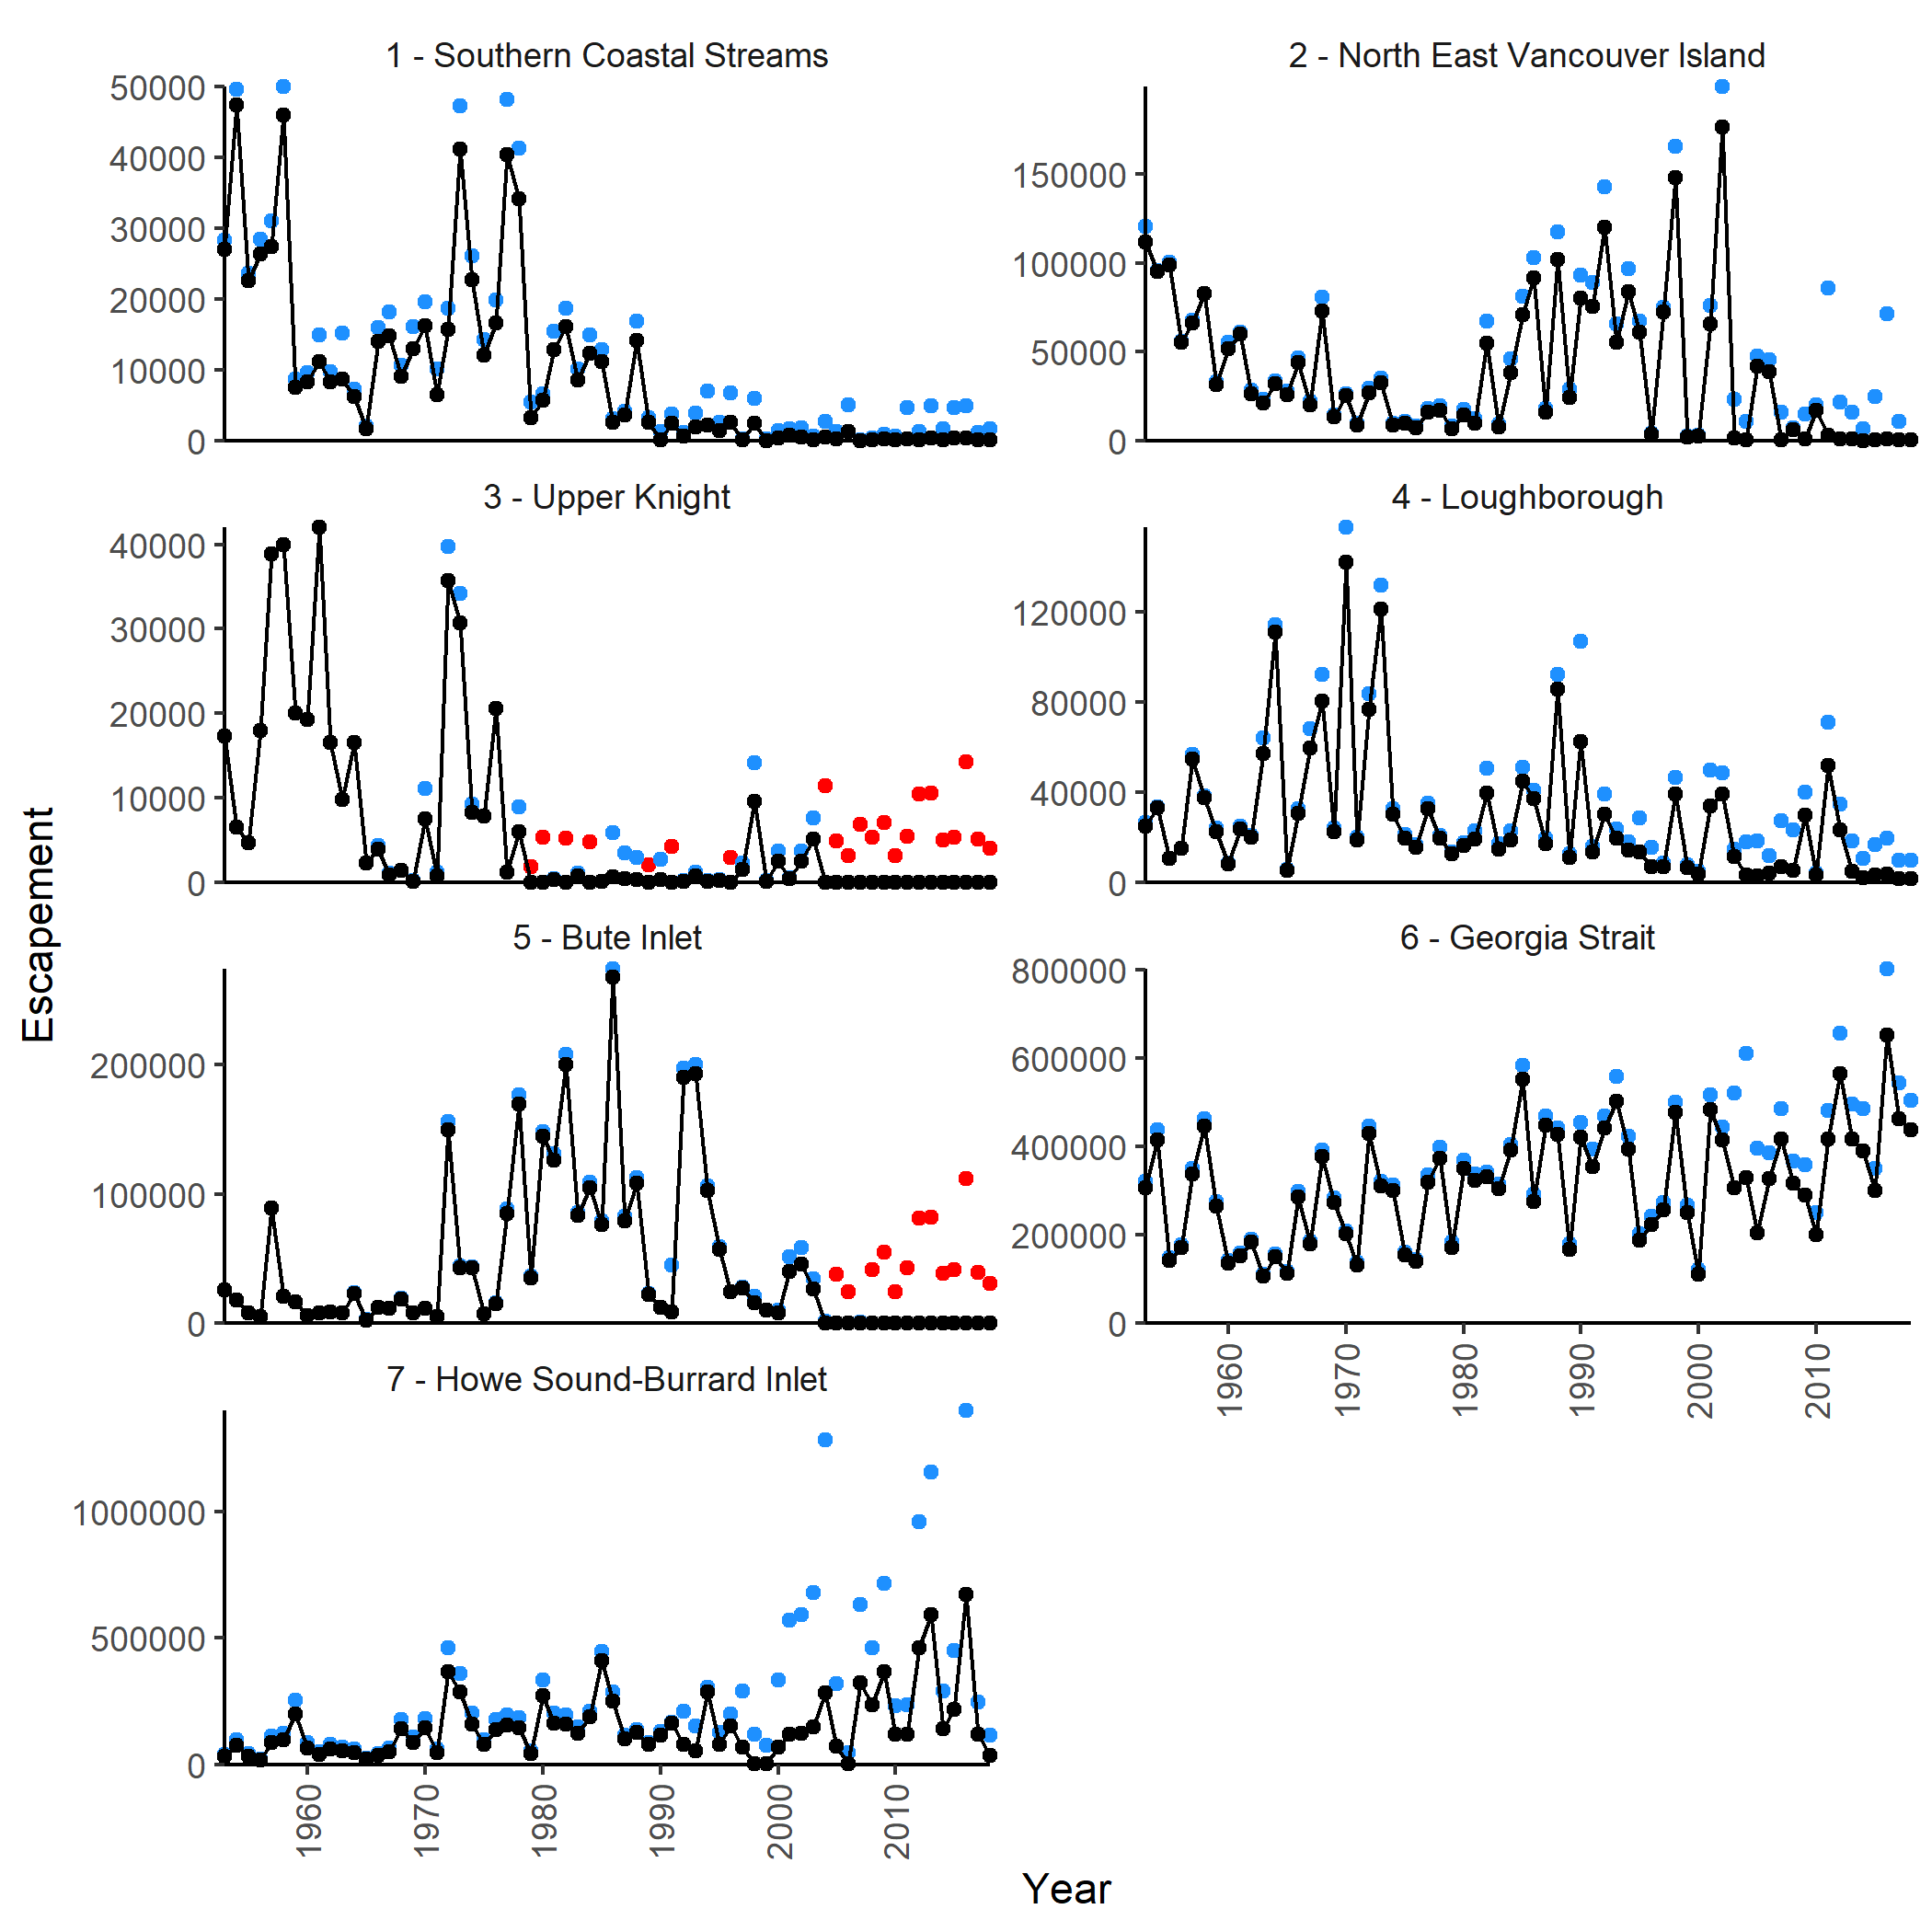
\includegraphics[width=6in]{figure/chum-escapement-infill}}{Figure \ref{fig:chum-escapement-infill}} 

}

\caption{Chum salmon escapement for the seven Conservation Units. Black points indicate actual counts, blue points are infilled by stream, and red points are infilled by Conservation Unit.}\label{fig:chum-escapement-infill}
\end{figure}
\hypertarget{run-reconstruction-to-estimate-recruitment}{%
\subsection{Run reconstruction to estimate recruitment}\label{run-reconstruction-to-estimate-recruitment}}

We reconstructed the returns for each brood year to give recruits for brood years 1955-2012 (age composition data from 1958-2018, minimum fish age was 3 years, maximum fish age was 6 years). Using CU benchmarks based on stock-recruit parameters - in this case, Sgen - requires knowing the spawners and recruits (adult offspring produced by each brood year of spawners) for each brood year (spawning year). Estimating recruits requires knowing wild spawner escapement, number of wild fish caught in fisheries, and the age of these fish.

To get these estimates, total (wild and hatchery origin) spawners based on the infilling methods above (both stream and CU level infilling) were calculated for each CU and Fishery Management Area (Figure~\ref{fig:chum-map}). The number of fish harvested in fisheries (wild and hatchery, by CU and Fishery Management Area) were added to the total escapement to get an estimate of totoal stock by CU and Fishery Management Area for each spawning year. This total stock number was multiplied by the proportion of wild spawners in each CU and Fishery Management Area based on the infilled wild and total spawner escapement. The product was an estimate of total wild stock (spawner escapement plus fishery harvest) by CU and Fishery Management Area for each brood year. Finally, the age composition of chum harvested in the Johnstone Strait aggregate fishery (ages 3, 4, 5 and 6) were used to assign fish from this total stock to brood years. As such, this analysis does not account for age diversity between CUs or streams.

Note that the two CUs requiring CU-level infilling correspond to only one Fishery Management Area each, which allows the run reconstruction using fishery harvest data at this level.
\begin{figure}[htb]

{\centering \pdftooltip{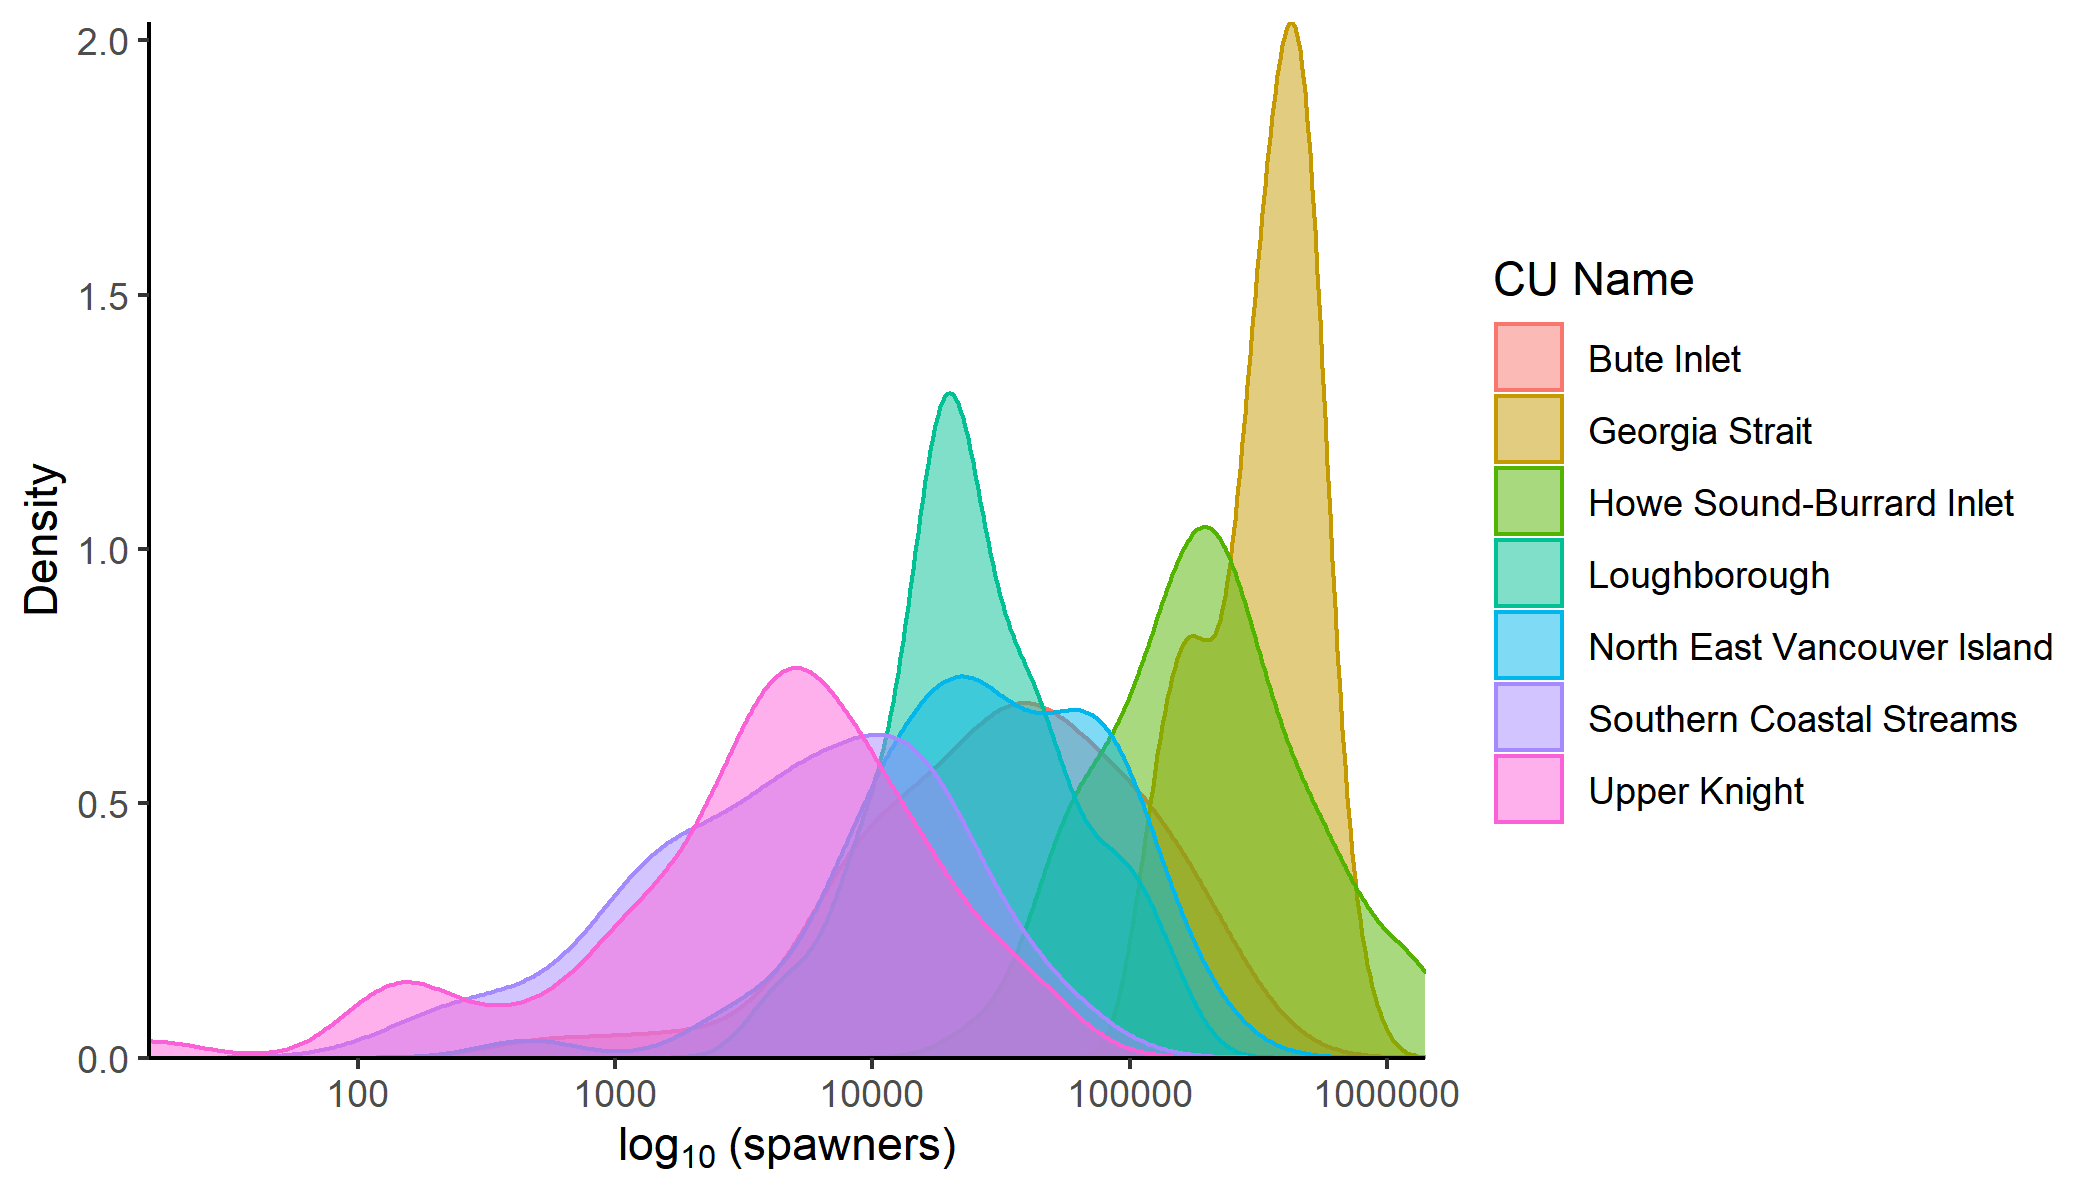
\includegraphics[width=6in]{figure/fig-spawner-dist}}{Figure \ref{fig:chum-spawner-distribution}} 

}

\caption{Density (smoothed histogram) of chum escapement for the seven Conservation Units. Note that x axis is on logarithmic scale.}\label{fig:chum-spawner-distribution}
\end{figure}

\clearpage

\refstepcounter{chapter}
\label{app:samsim-appendix}
\starredchapter{APPENDIX~\thechapter. samSim MODEL DOCUMENTATION}

\texttt{samSim} is the closed loop simulation modelling tool used for calculation of the projection-based LRPs. An overview of \texttt{samSim} and the code can be found in the LRP project \href{https://github.com/Pacific-salmon-assess/samSim/tree/LRP}{github page}. samSim has been previously used to evaluate harvest control rule performance relative to recovery potential ((\protect\hyperlink{ref-holtQuantitativeToolEvaluating2020}{Holt et al. 2020}; \protect\hyperlink{ref-freshwaterBenefitsLimitationsIncreasing2020}{Freshwater et al. 2020})). We created a modified version of samSim to support LRP estimation for this paper. Updated functionality for the LRP version of samSim include:
\begin{itemize}
\item
  The option to sample stock recruitment parameter sets directly from an estimated Bayesian joint posterior distribution.
\item
  The addition of a stock recruitment function that includes an environmental co-variate, as well as specification of future variability in the environmental co-variate (required for Interior Fraser Coho case study).
\item
  The option to initialize population dynamics for individual CUs at unfished equilibrium when no historical recruitment data are available. While this option would not be appropriate for projections aimed at estimating recovery from a current state, it can be used to estimate projection-based LRPs because we are only interested in the underlying relationship between aggregate abundance and the probability individual CUs will be above their lower benchmark.
\item
  The option to include a log-normal bias-correction factor of \(-\sigma^2 / 2\) to recruitment projected using one of the two available Ricker stock recruit models. This option was added to accommodate cases in which samSim is parameterized using stock recruitment parameters that have been corrected for log-normal bias to represent expected (mean) parameters. The log-nomral bias correction is commonly applied in stock recruit modelling because the expected value of \emph{e}\^{}\(\sigma\) is \emph{e}\^{}\(\sigma^2 / 2\)\} rather than zero when recruitment deviations are normally distributed (\protect\hyperlink{ref-coxCandidateLimitReference2019}{Cox et al.} (\protect\hyperlink{ref-coxCandidateLimitReference2019}{2019}), \protect\hyperlink{ref-ohlbergerBayesianLifecycleModel2019}{Ohlberger et al.} (\protect\hyperlink{ref-ohlbergerBayesianLifecycleModel2019}{2019}), \protect\hyperlink{ref-olmosEvidenceSpatialCoherence2019}{Olmos et al.} (\protect\hyperlink{ref-olmosEvidenceSpatialCoherence2019}{2019}), \protect\hyperlink{ref-forrestAssessmentPacificCod2020}{Forrest et al.} (\protect\hyperlink{ref-forrestAssessmentPacificCod2020}{2020}), Weir et al., in press). When input parameters have been corrected for this log-normal bias, the bias correction must also be added to projections. We use a log-normal bias correction factor for all of our case study analyses.
\item
  Specification of variability in exploitation rates as a function of both variability among years and variability among CUs.
\end{itemize}
This appendix describes the \texttt{samSim} model equations and the model's internal logic. We focus on providing detailed descriptions of the modeling options used for LRP study cases but include brief mentions of other model extensions already implemented within \texttt{samSim}. \texttt{samSim} includes two population scales, it could be applied to one Conservation Unit (CU) with component spawning populations, or one Stock Management Unit (SMU) with component CUs, or even one region with component SMUs. For the projection-based LRP analysis two SMUs and their component CUs were used as study cases: the West Coast of Vancouver Island (WCVI) Chinook SMU (with five CUs) and the Interior Fraser Coho Salmon SMU (with three CUs). The following sections in this appendix are organized similarly to the \texttt{samSim} code, for this reason the subheadings of this appendix can be read as pseudo code. The simulation model has two main phases: Model Priming and Projections. The model priming phase recreates data for past years, either by populating objects with observed data or by generating population trends based on input parameters. The projection phase generates data for future years based on the input data and parameters as well as the user defined scenarios and management procedures. The model indexes are defined in Table~\ref{tab:indtab}, the model parameters and model input are defined in Table~\ref{tab:paramtab} and the modeled quantities are defined in Table~\ref{tab:modtab}. Detailed definitions of the input data and parameters are provided in the project \href{https://github.com/Pacific-salmon-assess/samSim/tree/LRP\#readme}{README}.
\begin{table}[ht]
\centering
\caption{List of \texttt{samSim} model indexes.}
\begin{tabular}{l l}
\hline
Notation & Definition \\ 
\hline
$y$ & year \\ 
$nPrime$ & number of years in the priming phase\\
$Y$ & number of years in the projection phase\\
$j$ & age \\
$J$ & maximum age \\
$i$ & Conservation Unit (CU)\\
$I$ & Number of conservation units\\
$n$ & Nation: U.S. or Canada \\
\hline
\end{tabular}
\label{tab:indtab}
\end{table}
\begin{longtable}[]{l p{13.5cm}}
\caption{List of \texttt{samSim} model parameters and user input variables.}\\
\hline
Notation & Definition \\ 
\hline
\endhead
$\alpha_{i}$ & Ricker productivity parameter \\
$\beta_{i}$ & Ricker inverse capacity parameter \\
$\sigma_{i}$ & Standard deviation for recruitment error\\ 
$\rho$ & Temporal autocorrelation coefficient in recruitment residuals\\
$\gamma$ & Survival covariate scaler \\
$covMat$ & Covariance matrix used to generate recruitment deviations with correlation among CUs\\
$\overline{ER}_{n}$ & Nation specific long term average exploitation rate\\
$\overline{p}_{i,j}$ & Mean proportions of recruits at age\\
$\tau_{i}$ & Multivariate logistic variability parameter for proportions of recruits at age\\
$\overline{sv}$ & Mean survival covariate \\
$\sigma_{sv}$ & Standard deviation for survival covariate\\
$\Upsilon$ & Scalar to cap recruitment values \\
$\varphi$ & Multivariate logistic variability parameter for observed proportions of recruits at age\\
$\overline{\omega}$ & mean for forecast lognormal error\\
$\sigma_{\omega}$ & variance for forecast lognormal error\\
$CV(\overline{ER}_{n})$ & CV for MU-specific exploitation rate variability \\
$CV(ER_{y,i,n})$ & CV for CU-specific exploitation rate variability\\
$\psi$ & Proportion of the catch associated with mixed stock catch\\
$ERagg_{y,i}$ & Total exploitation rates\\
$\kappa$ & multivariate logistic variability parameter associated with assigning catch in mixed stock fisheries to the correct CU\\
$\hat{\alpha}_{y,i}$ & Estimated Ricker productivity parameter \\
$\hat{\beta}_{y,i}$ & Estimated Ricker inverse capacity parameter \\
\hline
\label{tab:paramtab}
\end{longtable}
\begin{longtable}[]{l p{13.5cm}}
\caption{List of \texttt{samSim} model variables.}\\
\hline
Notation & Definition \\ 
\hline
\endhead
\hline
$S_{y,i}$ & Spawners\\
$Seq_{i}$ & Equilibrium spawners\\
$RY_{y,i}$ & Calendar year recruitments\\
$p_{y,i,j}$ & Proportions of returns at age\\
$R_{y,i}$ & Brood year recruits \\
$Ra_{y,i,j}$ & Age spaecific brood year recruits\\
$w_{y,i}$ & Recruitment deviations with temporal auto-correlation\\
$v_{y,i}$ & Recruitment deviations\\
$sv_{y,j}$ & Brood year survival covariate\\
$svCY_{y}$ & Calendar survival covariate\\
$wsv_{y}$ & Survival covariate without bias correction\\
$Smsy_{i}$ & Spawners that produce the maximum sustainable yield \\
$Sgen_{i}$ & Number of spawners required to recover to $Smsy_{i}$ in one generation in the absence of fishing \\
${\alpha^\prime}_{i}$ & Adjusted $\alpha_{i}$ parameters for calculation of time invariant management benchmarks\\
$obsp_{y,i,j}$ & Observed proportions of recruits at age\\
$f(R_{y,i})$ &  Forecast of calendar year recruitment\\
$ER^{MU}_{y,n}$ & Exploitation rate including only MU-specific variability\\
$d1$, $d2$ & Shape parameters for Beta distribution used to generate MU-specific variability\\
$\vartheta$ & Standard deviation for MU-specific exploitation rate variability\\
$ER_{y,i,n}$ & Exploitation rate including MU- and CU-specific variability\\
$o1$, $o2$ & Shape parameters for Beta distribution used to generate CU-specific variability\\
$\phi_{y,i,n}$ & Standard deviation for CU-specific exploitation rate variability\\
${C}_{y,i,n}$ & Catch \\
${mC}_{y,i}$ & Mixed stock Canadian catches \\
${sC}_{y,i}$ & Single stock Canadian catches\\
$ERagg_{y,i}$ & Aggregate exploitation rates\\
${obsC}_{y,i,n}$ & Observed nation-specific catches \\
${obsmC}_{y,i}$ & Observed mixed stock Canadian catches\\
${obssC}_{y,i}$ & Observed single stock Canadian catches\\
$u_{y,i,n}$ & Lognormal error component of observed catches\\
$pCU_{y,i}$ & Proportion of catches from each CU\\
$obspCU_{y,i}$ & Observed proportion of catches from each CU \\
${obsS}_{y,i,n}$ & Observed spawners \\
$z_{y,i}$ & Lognormal error component of observed spawners\\
${obsRY}_{y,i,n}$ & Observed calendar year recruits \\
${obsER}_{y,i,n}$ & Observed exploitation rates \\
\hline
\label{tab:modtab}
\end{longtable}
\hypertarget{model-priming}{%
\appsection{MODEL PRIMING}\label{model-priming}}

The priming phase, or model initialization, represents the past data for CUs being modeled. It is used to represent true and observed abundances before starting the projection trials. This phase loops over a number of past years (`nPrime') and reconstructs recruitment time series for past years. The simulations can be initialized in two ways: with existing recruitment data or with user defined parameters, if recruitment data is not available.

\hypertarget{recruitment-data-is-available}{%
\subsection{Recruitment data is available}\label{recruitment-data-is-available}}

If spawner-recruitment data is available, the number of initialization years `nPrime' is defined based on the length of the longest CU time series available. The spawners, recruits, catch and exploitation rate objects are populated with the input data. If catch and/or exploitation rate data are not available, those values are set to zero.

\hypertarget{recruitment-data-is-not-available}{%
\subsection{Recruitment data is not available}\label{recruitment-data-is-not-available}}

When Recruitment data is not available, the `nPrime' is set to 10 times the maximum age of recruits. The first step on this routine is to retrieve the stock recruitment parameters. The user has the option of providing either one set of values to be used across all trials or many sets of parameter estimates, tipically from MCMC samples. If MCMC samples are provided, a different set of parameters is used for each simulation trial.

The spawner recruitment parameters can be altered according to the user defined scenarios, e.g.~to simulate regime shifts. \texttt{samSim} includes options to adjust the productivity parameter, \(\alpha_{i}\), the capacity parameter \(\beta_{i}\), and the recruitment standard deviations, \(\sigma_{i}\). The LRP case studies do not include adjustments or changes in productivity over time, therefore we will not describe the parameter adjustment options in this appendix. Recruitment is assumed to be correlated between the CUs, the covariance matrix is calculated based on the variance-covariance matrix, which is calculated based on CU-specific recruitment variances, and the correlation matrix specified in an input files.

Once stock-recruitment parameters are defined, the number of spawners is initialized. The number of spawners is set at equilibrium for the first 6 years (the maximum possible number of age classes) and then calculated based on recruitment and exploitation rates in the previous years (Equation~\ref{eq:Seqinit}). If the calculated number of spawners is lower than the user inputted extinction threshold, then the number of spawners is set to zero. Recruitment error is given by a multivariate normal distribution reflecting the recruitment covariance among CUs.
\begin{align}
S_{y,i} =
 \begin{cases}
   Seq_{i} &\text{ if } y = \leq 6\\
   RY_{y,i} \cdot (1 - \overline{ER}_{n}) &\text{ otherwise}
  \end{cases}
  \label{eq:Seqinit}
\end{align}
\begin{align}
Seq_{i} = \alpha_{i}/\beta_{i}
\label{eq:Seq}
\end{align}
The age structure of the returns is computed following a multivariate logistic error structure based on the long term average age structure for each CU, \(\overline{p}_{i,j}\) and the CU-specific variability parameter \(\tau_i\) (\protect\hyperlink{ref-schnuteInfluenceErrorPopulation1995}{Schnute and Richards 1995}) (Equation~\ref{eq:mat}. The age structure error can vary or be held constant among CUs. Calendar year recruitment is only calculated after the sixth year of the priming phase. It is the product of the brood year recruitment and the age structure of the returns (Equation~\ref{eq:RY}.
\begin{align}
  p_{y,i,j} \sim \text{Multivariate Logistic}(\overline{p}_{i,j},\tau_{i}) \\
  \label{eq:mat}
\end{align}
\begin{align}
\text{if y>6}\\
  RY_{y,i} = \sum_j(R_{y-j,i} \cdot p_{y-j,i,j})
  \label{eq:RY}
\end{align}
The computation of brood year recruitment follows the recruitment curve of choice. For the LRP version of \texttt{samSim}, three options for the recruitment curve are available: a simple Ricker curve (equation~\ref{eq:Rickersimple} when \(\rho = 0\)), Ricker curve with temporal autocorrelation in recruitment error (equation~\ref{eq:Rickersimple}), and Ricker curve with a smolt-to-adult marine survival covariate (Equations~\ref{eq:Rickersurv} and~\ref{eq:Rickersurvsum}, also described in Chapter~\ref{IFCChapter}). Recruitment error is assumed to be correlated among CUs for all versions of the Ricker curve. Random recruitment deviates can be generated with multivariate t or multivariate normal distributions, that can be symmetric or skewed. The study cases used in this report all assume that recruitment deviates come from a symmetrical multivariate normal distribution (Equation~\ref{eq:CUautocorr}).
\begin{align}
  R_{y,i} &= S_{y,i} \cdot e^{\alpha{i} - \beta{i} \cdot S_{y,i} + w_{y,i} - \frac{\sigma_{i}^{2}}{2}}\\
  \label{eq:Rickersimple}
\end{align}
\begin{align}
 w_{y,i} = 
\begin{cases}
 v_{y,i} & \text{if } y = 1 \\
 w_{y-1,i} * \rho + v_{y,i} & \text{if } y > 1
\end{cases}
\end{align}
\begin{align}
  v_{y,i} \sim N(\mu=0,covMat)
  \label{eq:CUautocorr}
\end{align}
\begin{align}
  Ra_{y,i,j} &= p_{y,i,j} \cdot S_{y,i} \cdot e^{\alpha_{i} - \beta_{i} \cdot S_{y,i} + \gamma_{i} \cdot sv_{y,j} + v_{y,i} - \frac{\sigma_{i}^{2}}{2}}
  \label{eq:Rickersurv}
\end{align}
\begin{align}
  R_{y,i} &= \sum_{j}Ra_{y,i,j}
  \label{eq:Rickersurvsum}
\end{align}
For the Ricker model with the marine survival covariate, the covariates for each calendar year are generated following a normal distribution with user defined mean and variance (Equation~\ref{eq:survCY}). The distribution of survival covariates is truncated between maximum and minimum values provided in the input files. The brood year survival covariates, \(Surv_{y,j}\), are currently populated following the dominant life history types from Interior Fraser Coho. For that stock, fish with a 3-year life cycle differ from those with a 4-year life cycle in the number of years spent in freshwater as juveniles, i.e., 18 months vs 30 months; both life cycles spend 18 months at sea before returning to spawn. Fish with a 2-year life cycle spend 18 months in the freshwater environment and only 6 months at sea before returning as jacks. This life history results in the survival covariate being lagged by one year for ages 2 and 3 Equation~\ref{eq:surv}). The exception is the first two years of the priming loop, when no lag is applied to the covariates.
\begin{align}
sv_{y,j} = 
\begin{cases}
 svCY_{y-1} & \text{if } j\leq 3 \\
 svCY_{y} & \text{otherwise}
\end{cases}
 \label{eq:surv}
\end{align}
\begin{align}
  svCY_{y} &= wsv_{y} - \dfrac{{\sigma_{sv}}^2}{2}\\
  wsv_{y} &\sim N(\overline{sv},\sigma_{sv})
  \label{eq:survCY}
\end{align}
Recruitment numbers produced with either formulation of the Ricker model are capped. The default maximum recruitment value is \(3 \cdot S_{eq}\), but the scalar can be modified by the user via the \(\Upsilon\) variable (Equation~\ref{eq:reccapscalar}). In addition, if the generated recruitment is lower than the user defined extinction threshold, then recruitment is set to zero.
\begin{align}
  R_{y,i} = min(R_{y,i}, \Upsilon \cdot Seq_{i})
  \label{eq:reccapscalar}
\end{align}
\hypertarget{compute-management-quantities-and-benchmarks}{%
\subsection{Compute management quantities and benchmarks}\label{compute-management-quantities-and-benchmarks}}

In the priming loop, the management quantities and benchmarks are only calculated in the last two generations. The management benchmarks are calculated according to three options: ``stockRecruit,'' ``percentile'' and ``habitat.'' \texttt{samSim} has the capability of estimating management quantities and benchmarks on a yearly basis, relying on the data obtained from the beginning of the time series to the current simulation year. However for the purpose of the LRP study cases, time invariant management benchmarks were used. For this reason we omit the time index, \(y\), from the notation used for the management quantities.

If the ``stockRecruit'' option is used, the management quantities are \(Smsy_{y,i}\) and \(Sgen_{y,i}\) calculated based on the stock-recruitment parameters. When the model with the survival covariate is used, the \(\alpha_{i}\) parameter is modified to incorporate the survival component (Equation~\ref{eq:alphamb}). In order to keep the management benchmarks constant through time, the long term average of the survival covariate is used. \(Smsy_{i}\) is calculated following the explicit solution provided by \protect\hyperlink{ref-scheuerellExplicitSolutionCalculating2016}{Scheuerell} (\protect\hyperlink{ref-scheuerellExplicitSolutionCalculating2016}{2016}) using the Lambert W function (Equation~\ref{eq:smsysamsim}). \(Sgen_{i}\) is estimated by solving Equation~\ref{eq:Sgensamsim} numerically, as described by \protect\hyperlink{ref-holtIndicatorsStatusBenchmarks2009}{Holt et al.} (\protect\hyperlink{ref-holtIndicatorsStatusBenchmarks2009}{2009}). The Lower management benchmark is set to \(Sgen_{y,i}\) and the upper benchmark is set to 80\% of \(Smsy_{y,i}\).
\begin{align}
{\alpha^\prime}_{i} =
\begin{cases}
\alpha_{i} + \gamma_{i}\cdot \overline{sv} & \text{for Ricker with survival} \\
\alpha_{i}  & \text{for simple Ricker}
\end{cases}  
  \label{eq:alphamb}
\end{align}
\begin{align}
  Smsy_{i} &= \dfrac{1 - W(e^{1-{\alpha^\prime}_{i}})}{\beta_{i}}
  \label{eq:smsysamsim}
\end{align}
\begin{align}
  Smsy_{i} = Sgen_{i} \cdot e^{{\alpha^\prime}_{i}\cdot \left( 1-\dfrac{Sgen_{i}}{\beta_{i}}\right)}
  \label{eq:Sgensamsim}
\end{align}
If the ``percentile'' benchmark option is chosen, the upper benchmark is set to the 50\textsuperscript{th} percentile of historical spawners (\(S_{1:y,i}\)). The lower benchmark is set to the 25\textsuperscript{th} percentile of historical spawners. If the ``habitat'' benchmark option is chosen, the benchmarks are computed using the same approach as in the ``stockRecruit'' option. The difference is in the origin of the stock recruit parameters, i.e., from the habitat model instead of spawner-recruitment curve.

\hypertarget{infill-missing-data}{%
\subsection{Infill missing data}\label{infill-missing-data}}

The last step of the model priming is infilling, which is only relevant if stock recruitment data is available and there are gaps in the last 12 years of the time series. Any gaps in the last 12 years of the Spawners and Recruits time series are infilled with a geometric mean of the entire priming period. In the priming phase, we assume that all variables are known without error, therefore all observations are set to the true simulation values, i.e., no observation error is added.

\hypertarget{model-projections}{%
\appsection{MODEL PROJECTIONS}\label{model-projections}}

The model projection phase is used to represent future potential outcomes. The steps in this phase will depend on the scenarios and management procedures selected by the user, and therefore will vary depending on the model application. In the following section, we list all steps in the order they appear in the code and indicate in the text if the step was used for the LRP case studies. Similarly to the priming phase, the subheadings in this section can be read as pseudocode. The projections run for each trial from year \texttt{nPrime\ +\ 1} to \texttt{Y}, the latter being the number of projection years defined by the user.

\hypertarget{specify-stock-recruitment-parameters}{%
\subsection{Specify stock recruitment parameters}\label{specify-stock-recruitment-parameters}}

Similarly to the priming phase, the first step on the projection loop is to define the stock recruitment parameters. The \(\beta_{i}\) and \(\sigma_{i}\) parameters are fixed through time and were already defined in the priming phase. However, if the user specifies productivity changes through time, then the productivity parameter \(\alpha{y,i}\) is adjusted every year following a linear trend. A detailed description of the algorithm used to generate productivity trends is out of the scope of this report as the study cases do not include scenarios with productivity changes. As the productivity parameter is held constant in the study cases, we will continue to use the time-invariant notation (\(\alpha_{i}\)) for the parameter in the sections to follow.

\hypertarget{project-management-benchmarks}{%
\subsection{Project management benchmarks}\label{project-management-benchmarks}}

Once \(\alpha_{i}\) is specified, the true management quantities \(Smsy_{i}\) and \(Sgen_{i}\) for the projection year are computed following Equations~\ref{eq:smsysamsim} and~\ref{eq:Sgensamsim}. The management benchmarks can be re-estimated every year or set by the normative period, i.e., last year of the priming phase, \texttt{nPrime}. The study cases in this report use the normative period management benchmarks.

\hypertarget{project-observed-recruitment}{%
\subsection{Project observed recruitment}\label{project-observed-recruitment}}

In this step, we compute the observed proportions of returns at age and the observed recruitment for each brood year. The observation error for the proportions of returns at age is given by a multivariate logistic error structure as described by \protect\hyperlink{ref-schnuteInfluenceErrorPopulation1995}{Schnute and Richards} (\protect\hyperlink{ref-schnuteInfluenceErrorPopulation1995}{1995}). Observation error for the proportions of returns at age is not included in the LRP study cases, i.e., the variability parameter, \(\varphi\), is set to zero.
\begin{align}
  obsp_{y,i,j} \sim \text{Multivariate Logistic}(p_{y,i,j}, \varphi) 
  \label{eq:obsppn}
\end{align}
The observed recruitment by brood year is retrieved by multiplying the true recruitment at age for each calendar year by the vector of observed proportions at age in the returns (Equation~\ref{eq:obsR}).
\begin{align}
  obsR_{y-j,i} &= \sum^j (RY_{y-j,i} \cdot obsp_{y-j,i,j})
  \label{eq:obsR}
\end{align}
\hypertarget{project-recruitment-forecast}{%
\subsection{Project recruitment forecast}\label{project-recruitment-forecast}}

When forecast error is included in the projection scenarios, it is generated by adding lognormal error around the calendar year recruitment (Equations~\ref{eq:FctR} and~\ref{eq:Fct}). The error distribution is also truncated between the 0.0001 and 0.9999 quantiles to avoid extreme forecast values. Forecast error is not considered in the LRP study cases.
\begin{align}
  f(RY_{y,i}) &= RY_{y,i} \cdot exp(\omega_{y,i})
  \label{eq:FctR}
\end{align}
\begin{align}
  \omega_{y,i} \sim N(\overline{\omega},\sigma_{\omega})
  \label{eq:Fct}
\end{align}
\hypertarget{project-realized-catches}{%
\subsection{Project realized catches}\label{project-realized-catches}}

The next step is to calculate the realized catches following a harvest control rule. Both study cases in this report use the fixed exploitation rate harvest control rule. In this option, the catch is the product of calendar year recruits and fixed exploitation rate over all projection years (Equation~\ref{eq:Catagg}). However, even though the harvest control rule specifies fixed exploitation rate, the realized exploitation rates vary from year to year due to changes in population distribution and fisheries dynamics. In this section we describe the layers of variability added to the simulated catches. Two layers of variability are considered in \texttt{samSim}, these represent MU-specific variability and CU-specific variability. Both uncertainty layers are implemented through draws of exploitation rate values from beta distributions. Currently only the Canadian catches include the annual added variability. In the LRP study cases, both U.S. Catches and Canadian single stock catches are set to zero, therefore only the Canadian mixed stock catches are implemented.

The first layer of catch variability is implemented at the MU level. The error is assumed to be the same for all CUs within an MU. The mean and variance for the MU level error are defined in the input files and then transformed into shape parameters for the Beta distribution draw (Equations~\ref{eq:ERMU}-\ref{eq:deER1} ).
\begin{align}
ER^{MU}_{y,n} 
\begin{cases}
  \sim Beta(d1,d2) & \text{n=Canada} \\
   = \overline{ER}_{n}  & \text{n=U.S.}
\end{cases}
  \label{eq:ERMU}
\end{align}
\begin{align}
\label{eq:deER1}
   d1 &= {\overline{ER}_{n}}^2 \cdot \left(\frac{1-\overline{ER}_{n}}{\vartheta^{2}}-\frac{1}{\overline{ER}_{n}}\right)  
\end{align}
\begin{align}
   d2 &= d1 \cdot \frac{1}{\overline{ER}_{n}-1}
\end{align}
\begin{align}
   \vartheta &= CV(\overline{ER}_{n}) \cdot \overline{ER}_{n}  
  \label{eq:deER}
\end{align}
In the second layer, CU-specific exploitation rates are drawn from a beta distribution using the output exploitation rate from the first layer as mean and CU-specific CV defined in the input files. The mean and CVs are transformed into shape parameters for the Beta distribution draws (Equations~\ref{eq:ERCU}-\ref{eq:oERCU}. The Catches are then computed by multiplying the CU specific \(ER\) and the calendar year recruits Equation~\ref{eq:Catagg}.
\begin{align}
ER_{y,i,n} 
\begin{cases}
 \sim Beta(o1_{y,i},o2_{y,i}) & \text{n=Canada} \\
 =\overline{ER}_{n}  & \text{n=U.S.}
\end{cases}  
  \label{eq:ERCU}
\end{align}
\begin{align}
   o1_{y,i} &= ({ER^{MU}_{y,n}})^2 \cdot \left(\frac{1-ER^{MU}_{y,n}}{\phi_{y,i,n}^{2}}-\frac{1}{ER^{MU}_{y,n}}\right)
\end{align}
\begin{align}
   o2_{y,i} &= o1_{y,i} \cdot \dfrac{1}{ER^{MU}_{y,n}-1}
\end{align}
\begin{align}
   \phi_{y,i,n} &= CV(ER_{y,i,n}) \cdot ER^{MU}_{y,n}
   \label{eq:oERCU}
\end{align}
\begin{align}
  {C}_{y,i,n} &= ER_{y,i,n} \cdot RY_{y,i}
  \label{eq:Catagg}
\end{align}
The catch for Canada is further divided in two components, mixed stock fishery and single stock fisheries (Equations~\ref{eq:tacmix} and~\ref{eq:tacsingle}).
\begin{align}
\label{eq:tacmix}
  {mC}_{y,i} &=  C_{y,i,n=Canada} \cdot \psi_{y,i} 
\end{align}
\begin{align}
  {sC}_{y,i} &= C_{y,i,n=Canada} \cdot (1- \psi_{y,i})
  \label{eq:tacsingle}
\end{align}
The next step is to compute the aggregate exploitation rate and the remaining number of Spawners (Equations~\ref{eq:eragg} and~\ref{eq:spawners}).
\begin{align}
  \label{eq:eragg}
  ERagg_{y,i} = \dfrac{\sum^n C_{y,i,n}}{RY_{y,i}}
\end{align}
\begin{align}
  S_{y,i} = RY_{y,i} \cdot(1-ERagg_{y,i}) 
   \label{eq:spawners}
\end{align}
\hypertarget{project-observed-data}{%
\subsection{Project observed data}\label{project-observed-data}}

In this step, observation error is added to the quantities calculated in the current time step. Catch observation error is given by a log normal distribution (Equations~\ref{eq:obsC}-\ref{eq:obssingleC}), the distribution is truncated between the 0.0001 and 0.9999 quantiles. If the catch is taken in a mixed stock fishery, additional multivariate logistic error is incorporated to account for uncertainty in the stock assignment process (Equation~\ref{eq:obspCU}).
\begin{align}
obsC_{y,i,n} =
 \begin{cases}
   C_{y,i,n} \cdot u_{y,i,n} &\text{ n=U.S.}\\
   {obsmC}_{y,i} +{obssC}_{y,i} &\text{ n=Canada}
  \end{cases}
  \label{eq:obsC}
\end{align}
Canadian mixed stock fisheries observed catches: \begin{align}
  {obsmC}_{y,i} &= {mC}_{y,i} \cdot u_{y,i,n} \cdot obspCU_{y,i} 
  \label{eq:obsmixC}
\end{align}
Canadian single stock fisheries observed catches:
\begin{align}
  {obssC}_{y,i} &= {sC}_{y,i} \cdot u_{y,i,n}
  \label{eq:obssingleC}
\end{align}
\begin{align}
u_{y,i,n} &\sim logN(0,\sigma_{C})
\end{align}
\begin{align}
  obspCU_{y,i}  &\sim \text{Multivariate Logistic}(pCU_{y,i},\kappa)
  \label{eq:obspCU}
\end{align}
\begin{align}
  pCU_{y,i} &= \dfrac{{mC}_{y,i}}{\sum^i {mC}_{y,i}}
\end{align}
Observed number of spawners is given by a log normal distribution truncated between the 0.0001 and 0.9999 quantiles (Equation~\ref{eq:obsS}). The observed recruitment is the sum of observed catches and observed spawner numbers (Equation~\ref{eq:obsRY}). The observed exploitation rate is directly calculated by dividing the observed catches by the observed recruitment (Equation~\ref{eq:obsER}).
\begin{align}
\label{eq:obsS}
  obsS_{y,i} &= S_{y,i} \cdot  \cdot z_{y,i}
\end{align}
\begin{align}
\label{eq:obsSz}
  z_{y,i} &\sim logN(0,\sigma_{S})
\end{align}
\begin{align}
  obsRY_{y,i} &= \sum^{n}obsC_{y,i,n} + obsS_{y,i}
   \label{eq:obsRY}
\end{align}
\begin{align}
  obsER_{y,i} &= \frac{\sum_{n}obsC_{y,i,n}}{obsRY_{y,i}}
  \label{eq:obsER}
\end{align}
\hypertarget{run-stock-assessment-and-calculate-management-quantities}{%
\subsection{Run stock assessment and calculate management quantities}\label{run-stock-assessment-and-calculate-management-quantities}}

This next phase of the projection loop simulates salmon stock assessment analysis. The linearized simple Ricker stock recruit curve is fit to the observed data and \(\hat{a}_{y,i}\) and \(\hat{b}_{y,i}\) are estimated.
\begin{align}
  log \left( \dfrac{obsR_{1:y,i}}{obsS_{1:y,i}}\right) &= \hat{\alpha}_{y,i}-\hat{\beta}_{y,i} \cdot  obsS_{y,i}\\
  \label{eq:obslogRS}
\end{align}
The management quantities, i.e., \(Sgen\) and \(Smsy\) or Spawners quantiles, can then be re-estimated based on the estimated stock recruitment parameters and the observed time series of spawners using the same procedure described in section~\ref{compute-management-quantities-and-benchmarks}. The LRP study cases, however, set the management benchmarks to the normative period, and for this reason the management quantities are kept constant and equal to the management benchmark at the last year of the priming period.

\hypertarget{project-population-dynamics}{%
\subsection{Project population dynamics}\label{project-population-dynamics}}

In this section the brood year recruitment for the current projection year is computed. The first step is to generate the marine survival estimates which are used to project recruitment when the Ricker model with survival covariates is used. The survival covariates are generated using the method described in Section~\ref{recruitment-data-is-not-available} and Equations~\ref{eq:survCY} and~\ref{eq:surv}. Marine survival covariates are considered to be constant across CUs.

The following step is compute the age structure of the returns with random error, which follows the same procedure described in Section~\ref{recruitment-data-is-not-available}. The age structure follows a distribution with mean age structure and standard deviation for each CU given in the input files.

In the next step, the recruitment deviations are computed with multivariate normal distribution, reflecting the recruitment covariance among CUs. Recruitment is then calculated following the same procedure described in Section\ref{recruitment-data-is-not-available} and using Equation~\ref{eq:Rickersimple} for the simple Ricker model, or Equation~\ref{eq:Rickersurv} for the Ricker model with survival covariates.

The last step of the projection loop is to compute the true and observed upper and lower benchmarks, which are based on the management quantities described in the previous section (Section~\ref{run-stock-assessment-and-calculate-management-quantities}. These are either stock-recruit or percentile benchmarks, as described in section~\ref{compute-management-quantities-and-benchmarks} computed based on the true and observed spawner abundances.


\clearpage

\refstepcounter{chapter}
\hypertarget{retrospective-analysis-of-cu-benchmarks-based-on-sgen-and-percentiles}{%
\starredchapter{APPENDIX~\thechapter. Retrospective analysis of CU benchmarks based on Sgen and percentiles}\label{retrospective-analysis-of-cu-benchmarks-based-on-sgen-and-percentiles}}

\emph{\textbackslash textcolor\{cyan\}\{LT: open to other name of this appendix}

In the retrospective analysis, the estimates of \(\alpha\), \(\beta\), and \(S_{gen}\) changed as progressively more years of data were included (Figures~\ref{fig:chum-a-b-SMSY-Sgen-retro}). Note that these are not estimates based on a model that accounts for time-varying parameters. Rather, the estimates of \(\alpha\), \(\beta\), and \(S_{gen}\) in a given year come from fitting a Ricker model to spawners and recruits for all years up to and including that year, for each CU. Each subsequent year includes another year of data. Thus, as more data is included, the estimates of \(\alpha\), \(\beta\), and \(S_{gen}\) may change. These results should be interpreted with caution due to the large residuals in observed vs.~predicted recruits. Since \(\alpha\) and \(\beta\) are correlated, the meaning of any trends in one parameter should be interpreted with the other parameter in mind, especially when model fits have large residuals. Similarly, since \(\alpha\) and \(\beta\) determine \(S_{MSY}\) and \(S_{gen}\), changes in these derived parameters can be challenging to interpret and can be due to changes in \(\alpha\), \(\beta\), and their relative values.
\begin{figure}[htb]

{\centering \pdftooltip{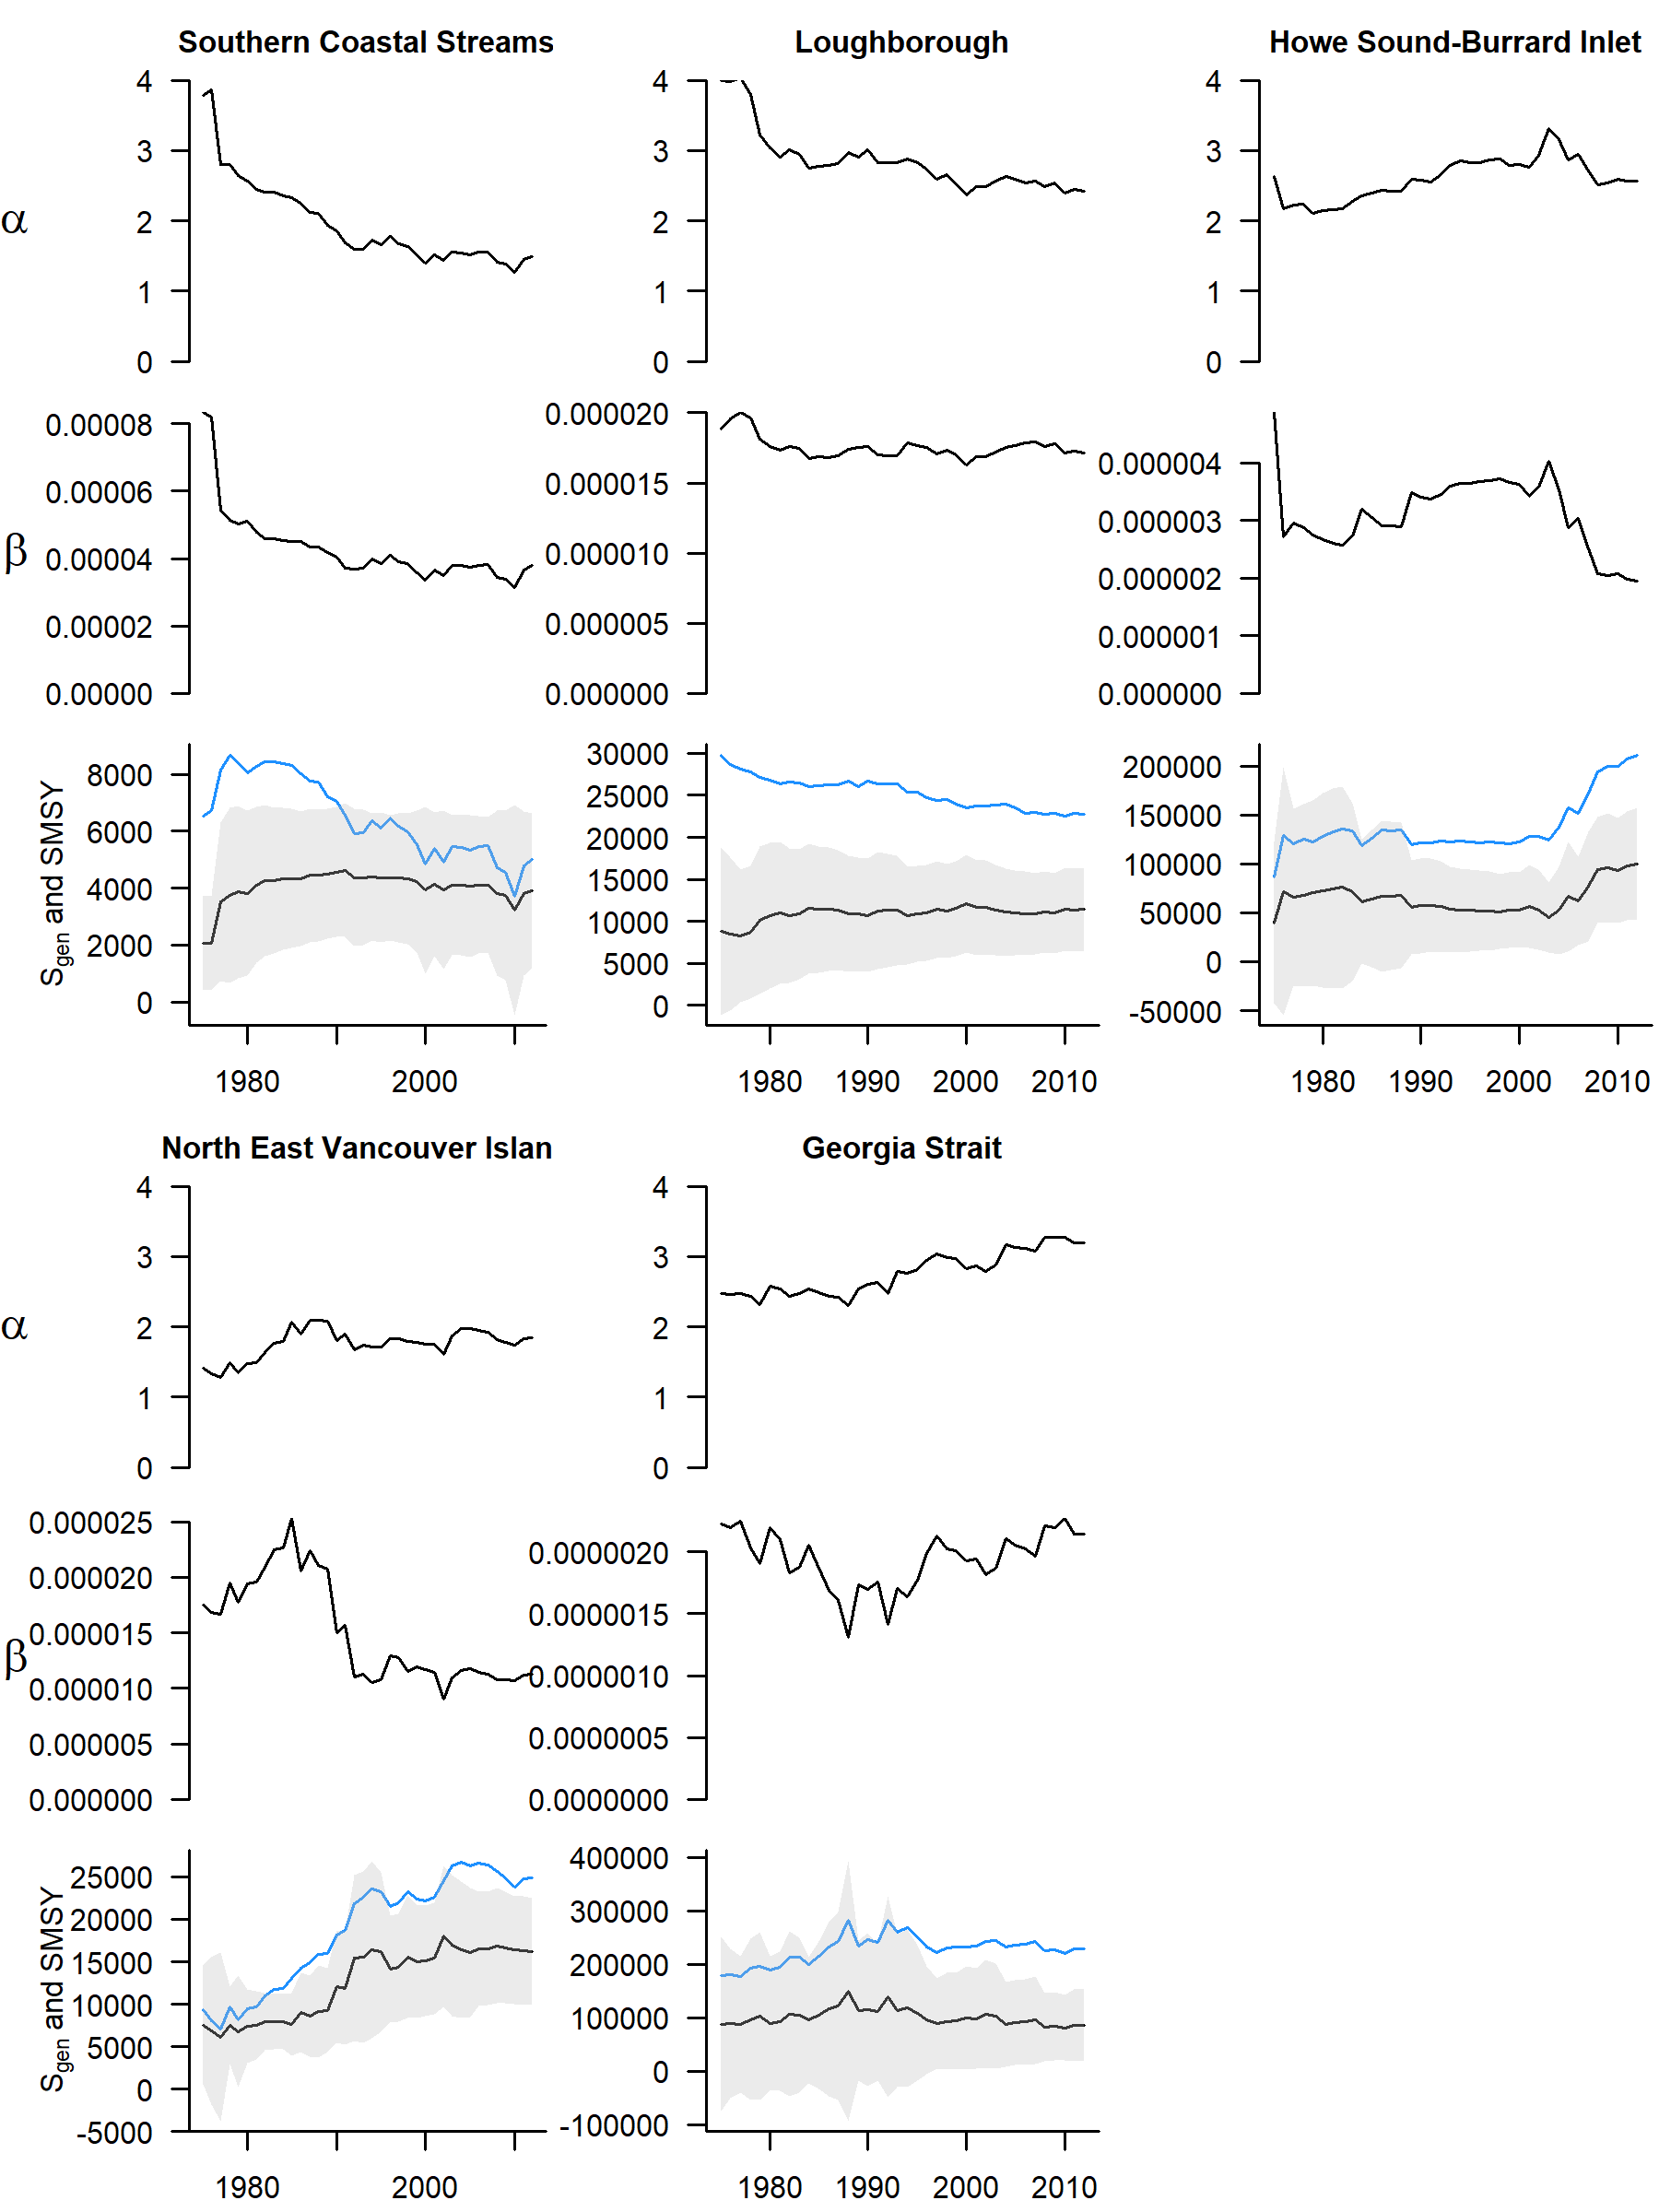
\includegraphics[width=6in]{figure/chum-a-b-SMSY-Sgen-retro}}{Figure \ref{fig:chum-a-b-SMSY-Sgen-retro}} 

}

\caption{Retrospective estimates of $\alpha$, $\beta$, $S_{gen}$ (black line with gray confidence intervals) and $S_{MSY}$ (blue line) for five CUs in the Inside South Coast Chum SMU. Note y axis is identical across CUs for $\alpha$ but varies for other parameters.}\label{fig:chum-a-b-SMSY-Sgen-retro}
\end{figure}
Retrospective estimates of \(\alpha\) and \(\beta\) for Southern Coastal Streams show declines over time. \(S_{MSY}\) and \(S_{gen}\) increase sharply in the first few years due to large decreases in \(\alpha\) and \(\beta\). \(S_{MSY}\) then decreases over time, while \(S_{gen}\) stays relatively stable. This is because as \(\alpha\) decreases below \textasciitilde2.5, \(S_{gen}\) decreases, but as \(\beta\) decreases, \(S_{gen}\) decreases, so that a simultaneous decrease in \(\alpha\) and \(\beta\) can cancel out. However, the lower alpha is below 2.5, the less influence \(\beta\) has on \(S_{gen}\). \emph{\textcolor{cyan}{This is from my work on sensitivity of Sgen and SMSY to alpha and beta. Not sure if we can include here}}

Increasing \(S_{gen}\) for North East Vancouver Island is mainly due to an increase in \(\alpha\) from \textless1.5 to \textgreater2 and then a decrease in \(\beta\).

\(\alpha\) for Loughborough showed modest decreases over time, and \(S_{gen}\) was fairly stable.

The Georgia Strait CU shows evidence of increasing \(\alpha\), and its \(S_{gen}\) estimate was fairly stable.

Howe Sound-Burrard Inlet \(S_{gen}\) was fairly stable, and then increased due to decreases in \(\alpha\) and \(\beta\).
\begin{figure}[htb]

{\centering \pdftooltip{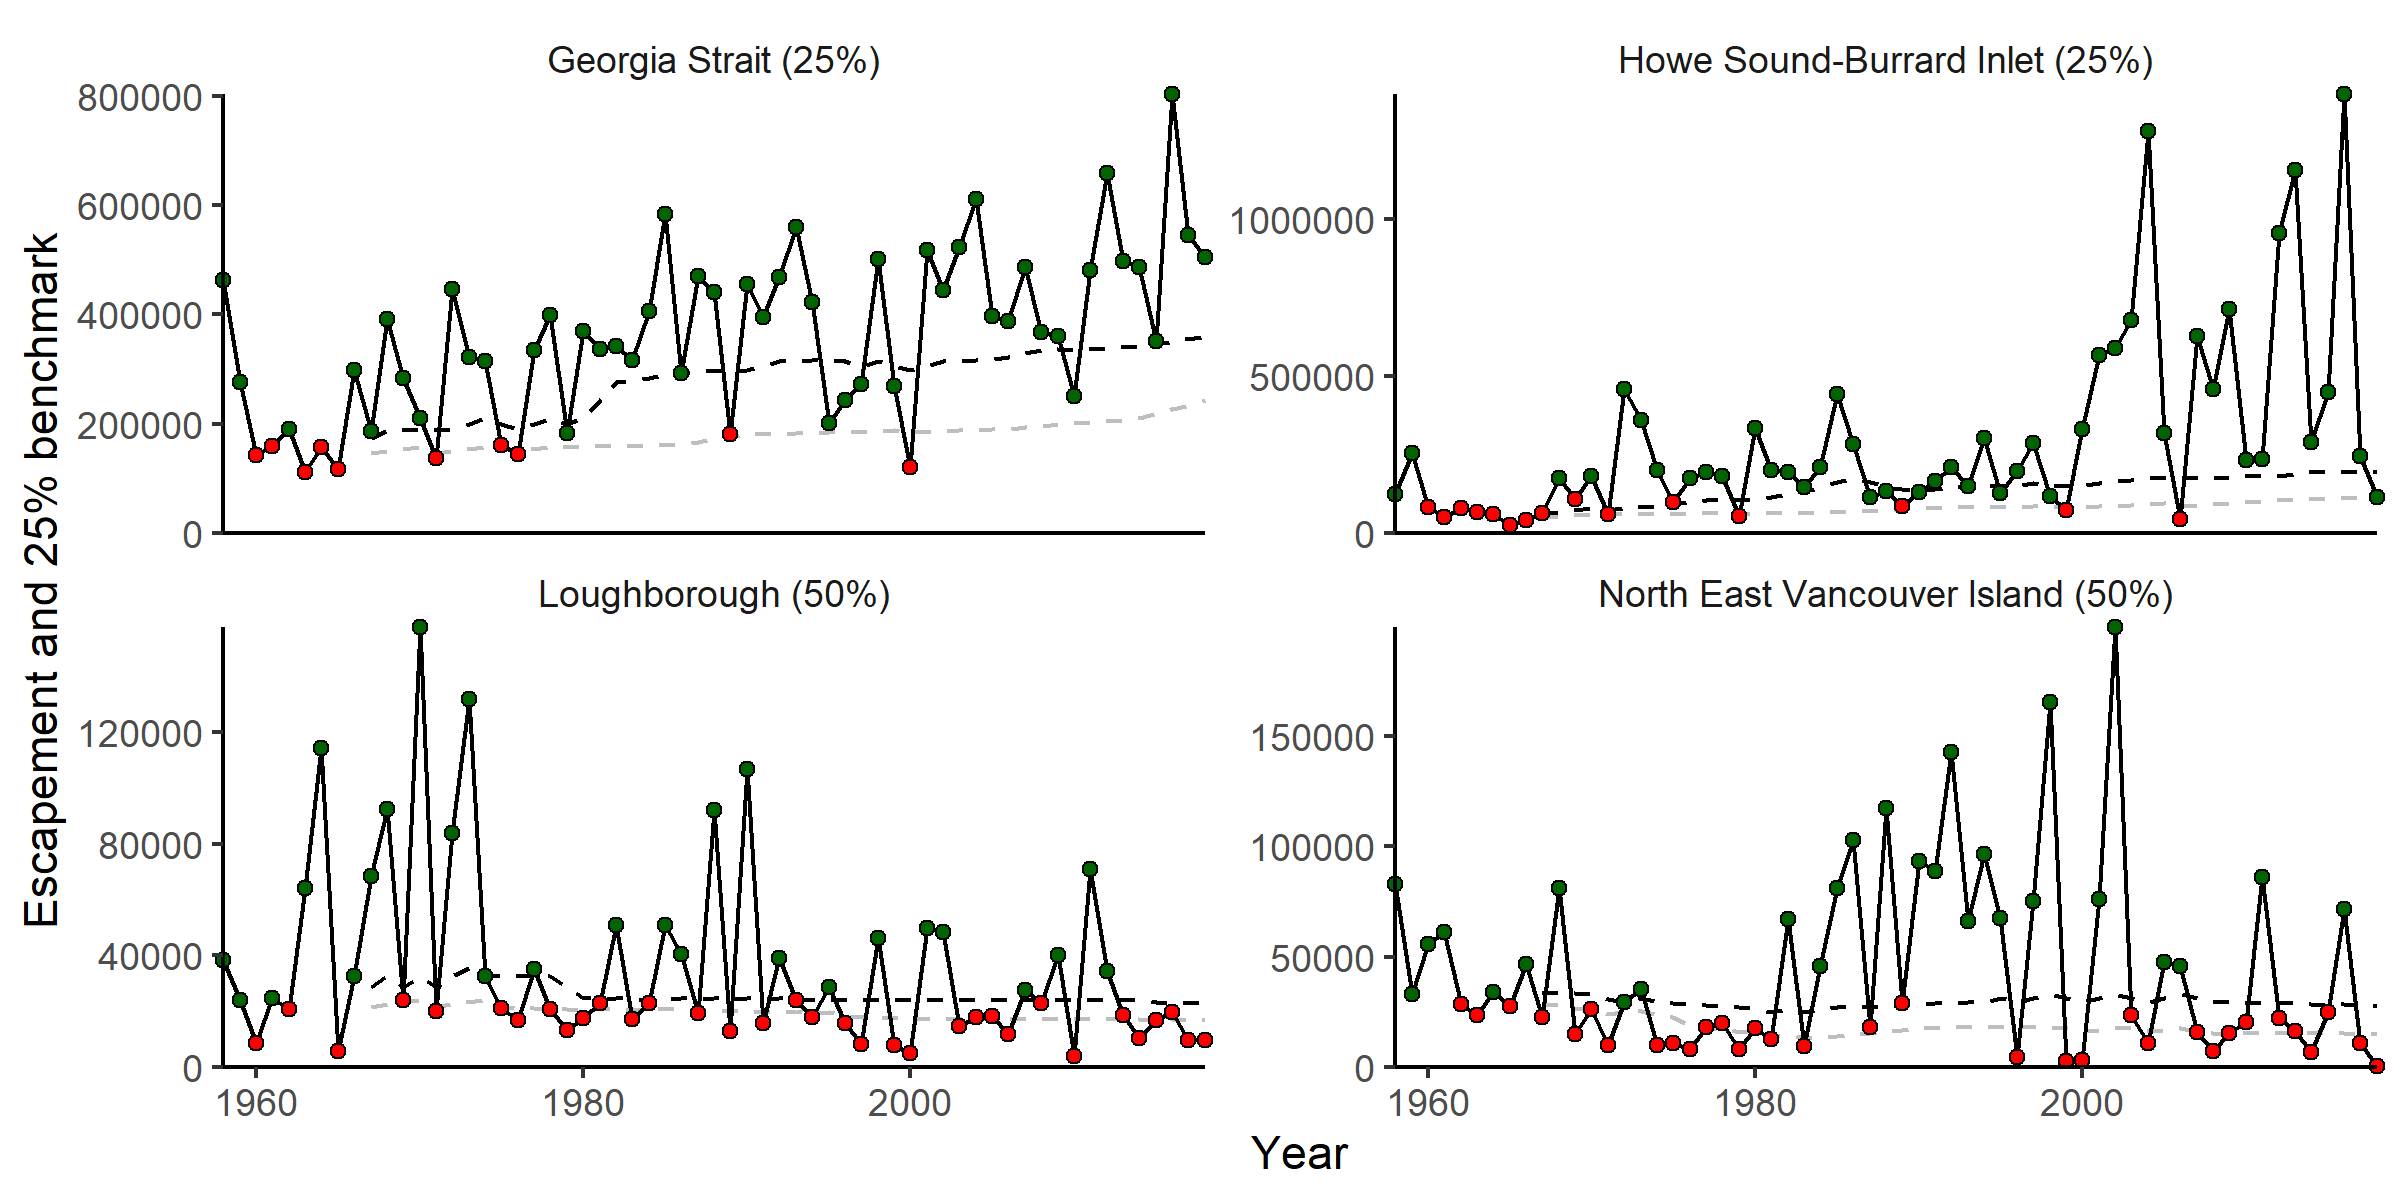
\includegraphics[width=6in]{figure/chum-perc-retro}}{Figure \ref{fig:chum-perc-retro}} 

}

\caption{Escapement with 25th and 50th percentile benchmarks shown by gray and black dotted lines, respectively. Benchmarks are calculated using escapements up to the given year. Values following the CU names indicate the appropriate percentile benchmark. Green and red points indicate status above or below benchmark, respectively. Transparent points are years with CU-level infilling.}\label{fig:chum-perc-retro}
\end{figure}
\begin{figure}[htb]

{\centering \pdftooltip{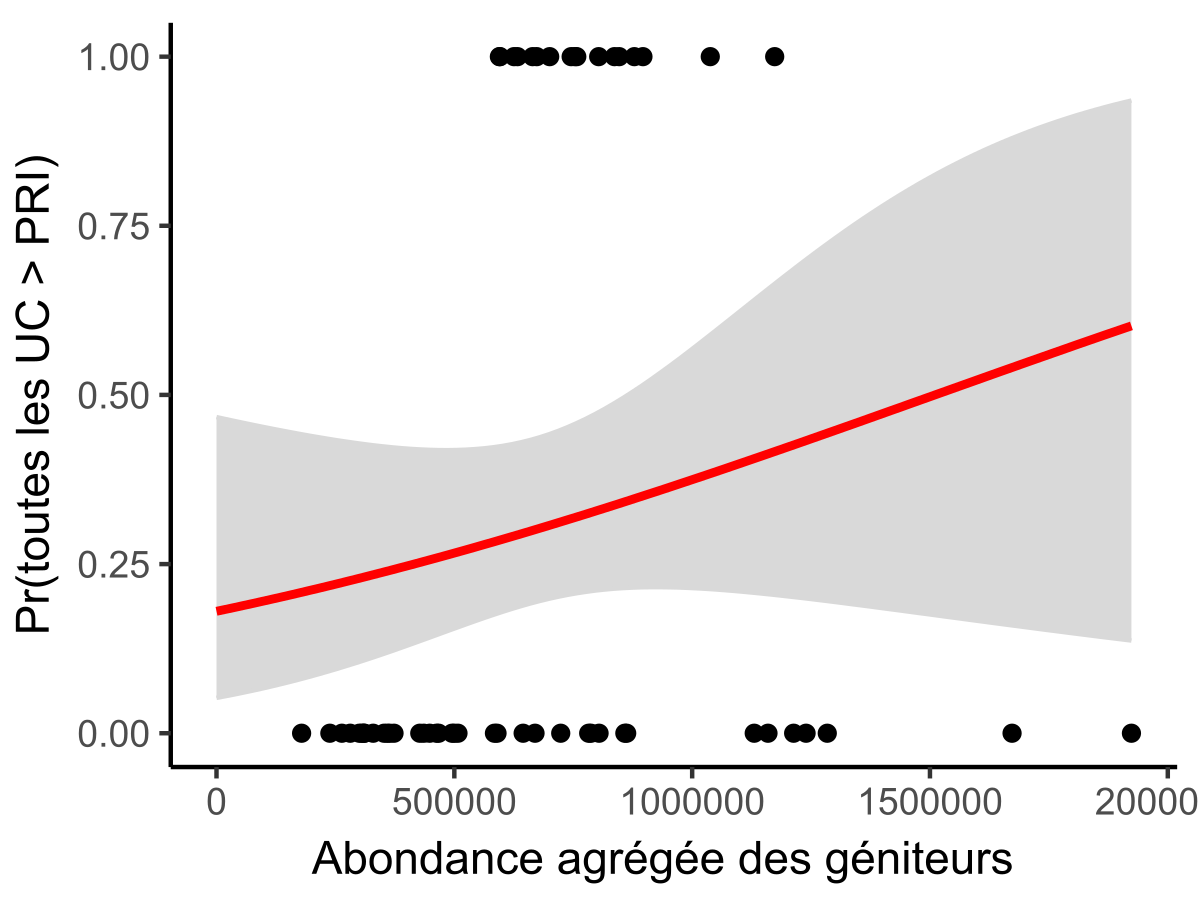
\includegraphics[width=6in]{figure/chum-logistic-sgen}}{Figure \ref{fig:chum-logistic-sgen}} 

}

\caption{Logistic regression of whether escapement of all component CUs were above their $S_{gen}$ benchmarks based on aggregate abundance, for Inside South Coast Chum SMU. Includes the 5 CUs without CU-level infilling (no Bute Inlet or Upper Knight)}\label{fig:chum-logistic-sgen}
\end{figure}

\clearpage

\refstepcounter{chapter}
\label{app:ERsensitivity-appendix}
\starredchapter{APPENDIX~\thechapter. Sensitivity of Projection-Based LRPs to Exploitation Rates}

To explain the initially counter-intuitive result of sensitivity of projection based LRPs to exploitation rates, we ran an additional analysis where the spawner-recruitment parameters, productivity (log(\(alpha\))) and spawners at replacement, \(S_{REP}\) (log(\(alpha\))/\(beta\)) were either varied or kept constant over inlets and Monte Carlo trials.

Specifically, we evaluated the sensitivity of aggregate projection-based LRPs to exploitation rates under three alternative scenarios:
\begin{enumerate}
\def\labelenumi{\arabic{enumi}.}
\item
  All inlets were assumed to have stock-recruitment parameters drawn from the same distributions (the mean and standard deviation for productivity and \(S_{REP}\) as estimated for Quatsino, Westcoast Vancouver Island) but a unique set of stock-recruitment parameters was drawn for each inlet and trial (i.e.~each inlet was a replicate of each other with random variability). We choose to draw \(S_{REP}\) from a random distributions instead of Ricker \(beta\) or \(S_{MAX}\) (1/\(beta\)) because the \(S_{REP}\) parameter was drawn randomly in projections for this case study from the watershed-area model. However, in preliminary sensitivity analyses, we sampled from a random distribution of \(beta\) values and found similar results. We assumed strong positive covariation in recruitment residuals among inlets with pairwise correlations equal to 0.7.
\item
  The productivity parameter was fixed at the mean value of the assumed distribution for all inlets and trials. \(S_{REP}\) was drawn from its distribution and allowed to vary across inlets and trials. The same distribution of \(S_{REP}\) was used across inlets and trials, as in Scenario 1.
\item
  \(S_{REP}\) was fixed at the mean value of the distribution across inlets and across trials. The productivity parameter was drawn from the distribution and allowed to vary across inlets and trials. The same distribution of productivity was used across inlets and trials, as in Scenario 1.
\end{enumerate}
We found that the sensitivity of projection-based LRPs to exploitation rates was due to variability in productivity and to a lesser extent \(S_{REP}\) among inlets. In Scenario 1, productivity and \(S_{REP}\) tended to be lower for random trials and inlets that dropped below the lower benchmark in at least one year. Random trials and inlets with abundances that remained above the lower benchmark over the time-series tended to be more productive and slightly larger (Fig.~\ref{fig:chinook-SRHistEven}).
\begin{figure}[htb]

{\centering \pdftooltip{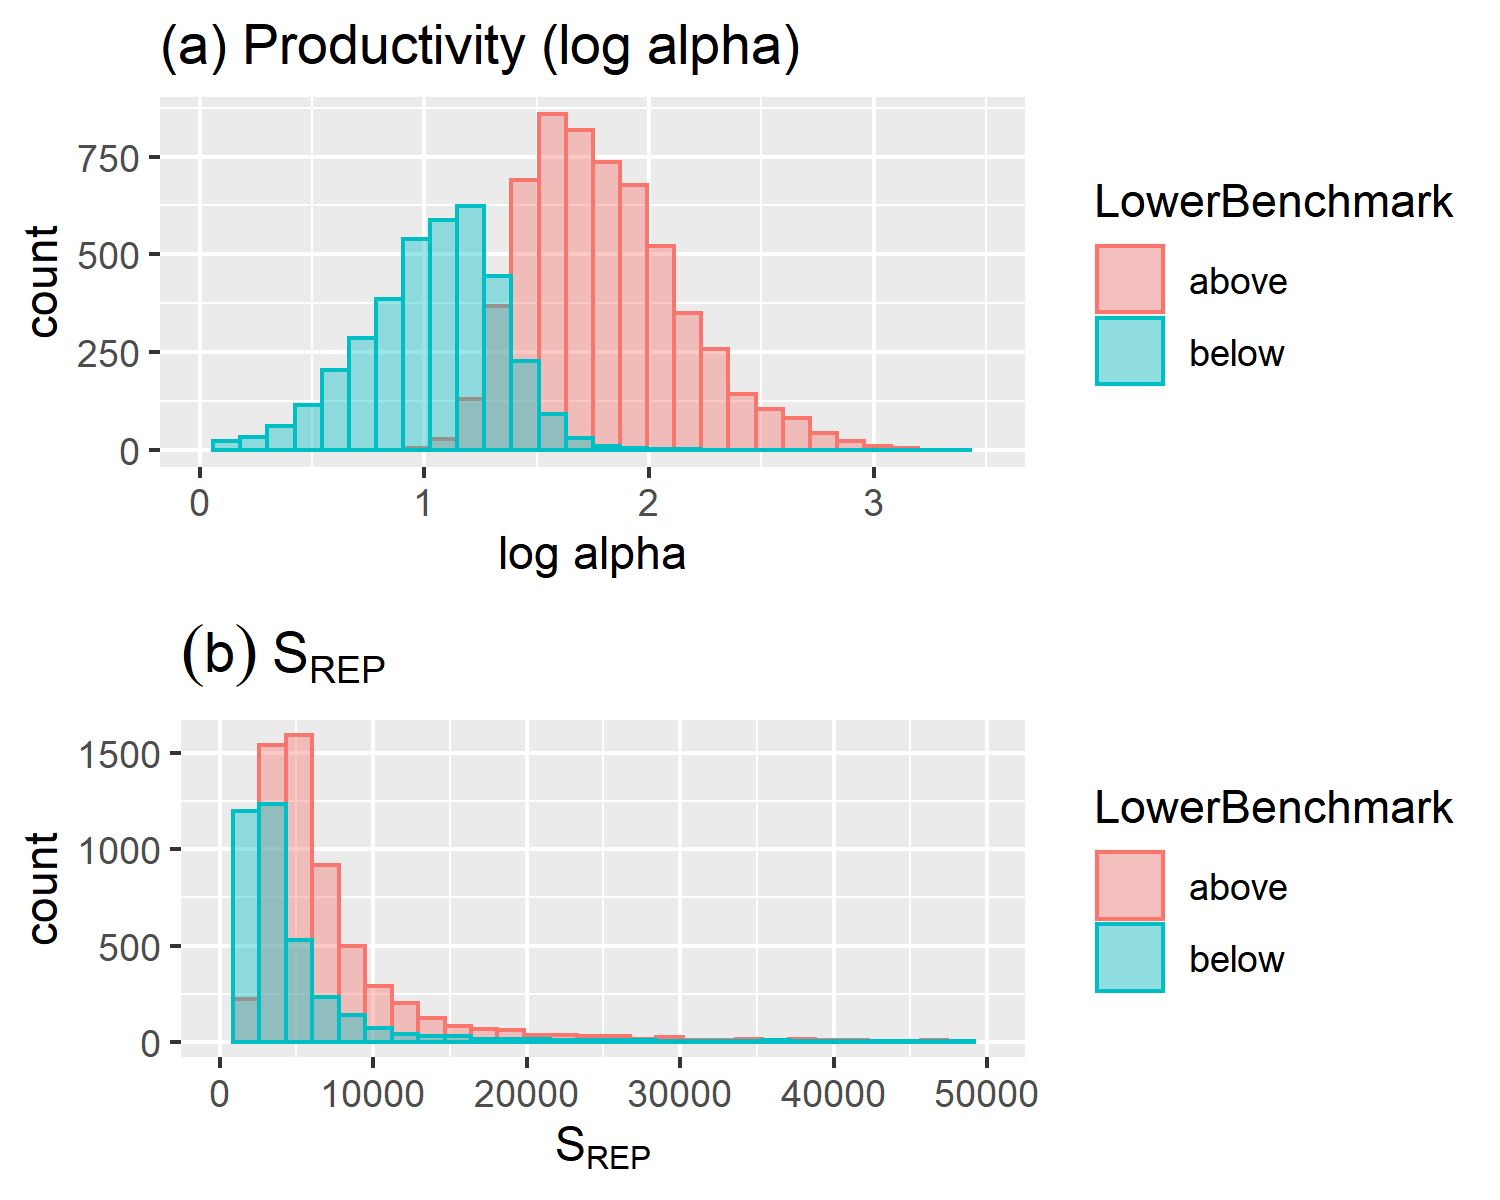
\includegraphics[width=6in]{figure/evenhCor-SRHist}}{Figure \ref{fig:chinook-SRHistEven}} 

}

\caption{Distribution of (a) productivity (log alpha) and (b) spawners at replacement, SREP among MC trials, coloured by whether abundances in that trial remained above the lower benchmark (red) or not (blue), under a 45\% exploitation. Productivity and SREP varied among inlets and trials and were drawn from common distributions. }\label{fig:chinook-SRHistEven}
\end{figure}
\linebreak

Inlets and Monte Carlo trials with low productivity tended to have relatively high \(S_{gen}\) (lower benchmark) values (as described in \protect\hyperlink{ref-holtCautionsUsingPercentilebased2015}{Holt and Folkes} (\protect\hyperlink{ref-holtCautionsUsingPercentilebased2015}{2015})), and therefore a higher frequency of dropping below the lower benchmark. This variability in productivity among inlets was associated with projection-based LRPs that were sensitive to exploitation rates (Fig.~\ref{fig:chinook-ProjLRPs-Even}).
\begin{figure}[htb]

{\centering \pdftooltip{\includegraphics[width=6in]{figure/ERsEven-hCor-ProjLRPCurve-ALLp}}{Figure \ref{fig:chinook-ProjLRPs-Even}} 

}

\caption{Probability of all inlets being above their lower benchmark along a gradient in aggregate abundances within bins of 200 fish, derived from projections over 30 years and 10,000 MC Trials, under a range of average exploitation rates from 5-45\%, assuming productivity and SREP varied across inlets and trials, and are drawn from common distributions. Horizontal dashed lines at 50\% and 66\% represent equal and likely probabilities of all inlets being above lower benchmarks. Orange and pale green vertical lines are the LRPs associated with 50\% and 66\% probability of all inlets being above their lower benchmarks, respectively. LRPs at 66\% probability are not shown for exploitation rates greater than 30\% because of large uncertainty in projections at high aggregate abundances.}\label{fig:chinook-ProjLRPs-Even}
\end{figure}
\linebreak

When productivity was fixed at the mean value among random trials and inlets in Scenario 2, the distribution of spawner-recruitment parameters for trials in which abundances dropped below the lower benchmark was the same or similar for trials that remained above it, and the LRP was insensitive to exploitation rate (Fig.~\ref{fig:chinook-SRHistSameProd} and~\ref{fig:chinook-ProjLRPs-SameProd}).
\begin{figure}[htb]

{\centering \pdftooltip{\includegraphics[width=6in]{figure/sameProdhCor-SRHist}}{Figure \ref{fig:chinook-SRHistSameProd}} 

}

\caption{Distribution of (a) productivity (log alpha) and (b) spawners at replacement, SREP among MC trials, coloured by whether abundances in that trial remained above the lower benchmark (red) or not (blue), under a 45\% exploitation and constant productivity among inlets and trials. SREP was drawn from a common distribution across inlets and trials. }\label{fig:chinook-SRHistSameProd}
\end{figure}
\begin{figure}[htb]

{\centering \pdftooltip{\includegraphics[width=6in]{figure/ERsSameProd-hCor-ProjLRPCurve-ALLp}}{Figure \ref{fig:chinook-ProjLRPs-SameProd}} 

}

\caption{Probability of all inlets being above their lower benchmark along a gradient in aggregate abundances within bins of 200 fish, derived from projections over 30 years and 10,000 MC Trials, under a range of average exploitation rates from 5-45\% (across 9 panels), assuming the same productivity for each inlet and trial and an SREP that varied across inlets and trials, drawn from a common distribution. Horizontal dashed lines at 50\% and 66\% represent equal and likely probabilities of all inlets being above lower benchmarks. Orange and pale green vertical lines are the LRPs associated with 50\% and 66\% probability of all inlets being above their lower benchmarks, but are indistinguishably here. }\label{fig:chinook-ProjLRPs-SameProd}
\end{figure}
\linebreak

When \(S_{REP}\) was fixed at the mean value among inlets and random trials in Scenario 3, productivity was higher for inlets and trials that remained above the benchmarks compared to those that dropped below them, though the overlap in the distributions above and below the lower benchmarks was slightly greater than when both \(S_{REP}\) and productivity varied (Scenario 1). The LRP varied with exploitation rates but to a lesser extent than when both productivity and \(S_{REP}\) varied (Fig.~\ref{fig:chinook-SRHistSameSREP} and~\ref{fig:chinook-ProjLRPs-SameSREP}).
\begin{figure}[htb]

{\centering \pdftooltip{\includegraphics[width=6in]{figure/sameSREPhCor-SRHist}}{Figure \ref{fig:chinook-SRHistSameSREP}} 

}

\caption{Distribution of (a) productivity (log alpha) and (b) spawners at replacement, SREP among MC trials, coloured by whether abundances in that trial remained above the lower benchmark (red) or not (blue), under a 45\% exploitation and constant SREP among inlets and trials. Productivity was drawn from a common distribution across inlets and trials. }\label{fig:chinook-SRHistSameSREP}
\end{figure}
\begin{figure}[htb]

{\centering \pdftooltip{\includegraphics[width=6in]{figure/ERsSameSREP-hCor-ProjLRPCurve-ALLp}}{Figure \ref{fig:chinook-ProjLRPs-SameSREP}} 

}

\caption{Probability of all inlets being above their lower benchmark along a gradient in aggregate abundances within bins of 200 fish, derived from projections over 30 years and 10,000 MC Trials, under a range of average exploitation rates from 5-45\% (across 9 panels), assuming the same SREP for each inlet and trial, and productivity that varied across inlets and trials, drawn from a common distribution. Horizontal dashed lines at 50\% and 66\% represent equal and likely probabilities of all inlets being above lower benchmarks. Orange and pale green vertical lines are the LRPs associated with 50\% and 66\% probability of all inlets being above their lower benchmarks, respectively. }\label{fig:chinook-ProjLRPs-SameSREP}
\end{figure}
\linebreak

Based on these sensitivity analyses, we conclude that variability in productivity among inlets results in inlet-specific variability in sensitivity to exploitation rates. Inlets with relatively low productivity fall below lower benchmarks more frequently. This effect is accentuated when exploitation rates are high resulting in divergences in status among inlets and a higher aggregate abundances required for all inlets to be above their lower benchmarks (i.e., higher LRP).


\clearpage

\refstepcounter{chapter}
\label{app:coho-appendix}
\starredchapter{APPENDIX~\thechapter. Interior Fraser Coho Model Fits}
\begin{figure}[htb]

{\centering \pdftooltip{\includegraphics[width=0.8\linewidth]{figure/coho-SrepPriorDist}}{Figure \ref{fig:coho-SrepPrior}} 

}

\caption{Prior distribution of SRep used when fitting the Ricker\_priorCap model.The red dashed line shows the maximum likelihood estimate of SRep from the base Ricker model stock recruitment fit. The mean of the SRep prior was set to 1.35 times the maximum likelihood estimate}\label{fig:coho-SrepPrior}
\end{figure}
To Do: improve table formatting; can I make font arial?
\begin{longtable}[]{@{}llrrrr@{}}
\caption{\label{tab:coho-postSummary-Ricker}Summary of posterior distribution mean and quantiles (5\%, 50\%, and 95\%) for stock recruit model parameters and Sgen lower benchmark from the Ricker model fit.}\tabularnewline
\toprule
CU & Variable & Mean & P05 & P50 & P95 \\
\midrule
\endfirsthead
\toprule
CU & Variable & Mean & P05 & P50 & P95 \\
\midrule
\endhead
Middle Fraser & adjProd & 2.380e+00 & 1.730e+00 & 2.320e+00 & 3.200e+00 \\
& alpha & 2.880e+00 & 2.200e+00 & 2.870e+00 & 3.620e+00 \\
& beta & 1.200e-04 & 7.000e-05 & 1.200e-04 & 1.700e-04 \\
& gamma & 4.200e-01 & 2.900e-01 & 4.200e-01 & 5.600e-01 \\
& Sgen & 1.646e+03 & 8.700e+02 & 1.576e+03 & 2.663e+03 \\
& sigma & 4.500e-01 & 3.400e-01 & 4.400e-01 & 6.000e-01 \\
Fraser Canyon & adjProd & 6.260e+00 & 3.160e+00 & 5.670e+00 & 1.121e+01 \\
& alpha & 3.790e+00 & 2.920e+00 & 3.770e+00 & 4.730e+00 \\
& beta & 4.200e-04 & 2.600e-04 & 4.200e-04 & 5.900e-04 \\
& gamma & 4.200e-01 & 2.900e-01 & 4.200e-01 & 5.600e-01 \\
& Sgen & 3.140e+02 & 5.200e+01 & 2.660e+02 & 7.480e+02 \\
& sigma & 7.600e-01 & 5.700e-01 & 7.400e-01 & 1.010e+00 \\
Lower Thompson & adjProd & 2.560e+00 & 1.570e+00 & 2.450e+00 & 3.960e+00 \\
& alpha & 2.930e+00 & 2.200e+00 & 2.930e+00 & 3.690e+00 \\
& beta & 1.000e-04 & 5.000e-05 & 1.000e-04 & 1.500e-04 \\
& gamma & 4.200e-01 & 2.900e-01 & 4.200e-01 & 5.600e-01 \\
& Sgen & 1.977e+03 & 9.700e+02 & 1.841e+03 & 3.429e+03 \\
& sigma & 5.900e-01 & 4.500e-01 & 5.800e-01 & 7.800e-01 \\
North Thompson & adjProd & 3.170e+00 & 2.290e+00 & 3.090e+00 & 4.290e+00 \\
& alpha & 3.170e+00 & 2.510e+00 & 3.160e+00 & 3.870e+00 \\
& beta & 8.000e-05 & 5.000e-05 & 8.000e-05 & 1.000e-04 \\
& gamma & 4.200e-01 & 2.900e-01 & 4.200e-01 & 5.600e-01 \\
& Sgen & 2.482e+03 & 1.557e+03 & 2.409e+03 & 3.650e+03 \\
& sigma & 4.100e-01 & 3.100e-01 & 4.100e-01 & 5.500e-01 \\
South Thompson & adjProd & 2.470e+00 & 1.590e+00 & 2.370e+00 & 3.660e+00 \\
& alpha & 2.910e+00 & 2.170e+00 & 2.890e+00 & 3.700e+00 \\
& beta & 8.000e-05 & 4.000e-05 & 8.000e-05 & 1.300e-04 \\
& gamma & 4.200e-01 & 2.900e-01 & 4.200e-01 & 5.600e-01 \\
& Sgen & 2.573e+03 & 1.291e+03 & 2.365e+03 & 4.667e+03 \\
& sigma & 5.700e-01 & 4.300e-01 & 5.600e-01 & 7.500e-01 \\
\bottomrule
\end{longtable}
\begin{longtable}[]{@{}llrrrr@{}}
\caption{\label{tab:coho-postSummary-RickerCap}Summary of posterior distribution mean and quantiles (5\%, 50\%, and 95\%) for stock recruit model parameters and Sgen lower benchmark from the Ricker\_prioCap model fit.}\tabularnewline
\toprule
CU\_Name & Variable & Mean & P05 & P50 & P95 \\
\midrule
\endfirsthead
\toprule
CU\_Name & Variable & Mean & P05 & P50 & P95 \\
\midrule
\endhead
Middle Fraser & adjProd & 2.290e+00 & 1.640e+00 & 2.220e+00 & 3.190e+00 \\
& alpha & 2.580e+00 & 1.870e+00 & 2.570e+00 & 3.350e+00 \\
& beta & 8.000e-05 & 4.000e-05 & 8.000e-05 & 1.300e-04 \\
& gamma & 3.700e-01 & 2.300e-01 & 3.600e-01 & 5.100e-01 \\
& Sgen & 2.515e+03 & 1.339e+03 & 2.452e+03 & 3.932e+03 \\
& sigma & 5.200e-01 & 3.900e-01 & 5.000e-01 & 6.900e-01 \\
Fraser Canyon & adjProd & 6.360e+00 & 3.240e+00 & 5.800e+00 & 1.127e+01 \\
& alpha & 3.550e+00 & 2.680e+00 & 3.530e+00 & 4.490e+00 \\
& beta & 4.265e-04 & 2.698e-04 & 4.258e-04 & 5.866e-04 \\
& gamma & 3.700e-01 & 2.300e-01 & 3.600e-01 & 5.100e-01 \\
& Sgen & 3.040e+02 & 5.300e+01 & 2.580e+02 & 7.150e+02 \\
& sigma & 7.500e-01 & 5.700e-01 & 7.400e-01 & 1.000e+00 \\
Lower Thompson & adjProd & 2.640e+00 & 1.570e+00 & 2.470e+00 & 4.240e+00 \\
& alpha & 2.700e+00 & 1.930e+00 & 2.680e+00 & 3.530e+00 \\
& beta & 7.000e-05 & 3.000e-05 & 7.000e-05 & 1.200e-04 \\
& gamma & 3.700e-01 & 2.300e-01 & 3.600e-01 & 5.100e-01 \\
& Sgen & 2.781e+03 & 1.241e+03 & 2.654e+03 & 4.767e+03 \\
& sigma & 6.700e-01 & 5.100e-01 & 6.600e-01 & 8.900e-01 \\
North Thompson & adjProd & 3.200e+00 & 2.150e+00 & 3.090e+00 & 4.620e+00 \\
& alpha & 2.910e+00 & 2.190e+00 & 2.900e+00 & 3.660e+00 \\
& beta & 6.000e-05 & 4.000e-05 & 6.000e-05 & 9.000e-05 \\
& gamma & 3.700e-01 & 2.300e-01 & 3.600e-01 & 5.100e-01 \\
& Sgen & 3.171e+03 & 1.771e+03 & 3.051e+03 & 5.017e+03 \\
& sigma & 5.000e-01 & 3.700e-01 & 4.900e-01 & 6.600e-01 \\
South Thompson & adjProd & 2.350e+00 & 1.540e+00 & 2.220e+00 & 3.560e+00 \\
& alpha & 2.590e+00 & 1.830e+00 & 2.570e+00 & 3.410e+00 \\
& beta & 5.000e-05 & 3.000e-05 & 5.000e-05 & 8.000e-05 \\
& gamma & 3.700e-01 & 2.300e-01 & 3.600e-01 & 5.100e-01 \\
& Sgen & 4.050e+03 & 2.130e+03 & 3.978e+03 & 6.247e+03 \\
& sigma & 6.400e-01 & 4.800e-01 & 6.200e-01 & 8.400e-01 \\
\bottomrule
\end{longtable}

\clearpage

\refstepcounter{chapter}
\label{app:github-appendix}
\starredchapter{APPENDIX~\thechapter. DATA AND ANALYSIS LINKS}

Data and analysis code for the ISC Chum case study are available at: \url{https://github.com/Pacific-salmon-assess/SalmonLRP_RetroEval}

\end{document}
